\documentclass[twoside]{book}

% Packages required by doxygen
\usepackage{fixltx2e}
\usepackage{calc}
\usepackage{doxygen}
\usepackage[export]{adjustbox} % also loads graphicx
\usepackage{graphicx}
\usepackage[utf8]{inputenc}
\usepackage{makeidx}
\usepackage{multicol}
\usepackage{multirow}
\PassOptionsToPackage{warn}{textcomp}
\usepackage{textcomp}
\usepackage[nointegrals]{wasysym}
\usepackage[table]{xcolor}

% Font selection
\usepackage[T1]{fontenc}
\usepackage[scaled=.90]{helvet}
\usepackage{courier}
\usepackage{amssymb}
\usepackage{sectsty}
\renewcommand{\familydefault}{\sfdefault}
\allsectionsfont{%
  \fontseries{bc}\selectfont%
  \color{darkgray}%
}
\renewcommand{\DoxyLabelFont}{%
  \fontseries{bc}\selectfont%
  \color{darkgray}%
}
\newcommand{\+}{\discretionary{\mbox{\scriptsize$\hookleftarrow$}}{}{}}

% Page & text layout
\usepackage{geometry}
\geometry{%
  a4paper,%
  top=2.5cm,%
  bottom=2.5cm,%
  left=2.5cm,%
  right=2.5cm%
}
\tolerance=750
\hfuzz=15pt
\hbadness=750
\setlength{\emergencystretch}{15pt}
\setlength{\parindent}{0cm}
\setlength{\parskip}{3ex plus 2ex minus 2ex}
\makeatletter
\renewcommand{\paragraph}{%
  \@startsection{paragraph}{4}{0ex}{-1.0ex}{1.0ex}{%
    \normalfont\normalsize\bfseries\SS@parafont%
  }%
}
\renewcommand{\subparagraph}{%
  \@startsection{subparagraph}{5}{0ex}{-1.0ex}{1.0ex}{%
    \normalfont\normalsize\bfseries\SS@subparafont%
  }%
}
\makeatother

% Headers & footers
\usepackage{fancyhdr}
\pagestyle{fancyplain}
\fancyhead[LE]{\fancyplain{}{\bfseries\thepage}}
\fancyhead[CE]{\fancyplain{}{}}
\fancyhead[RE]{\fancyplain{}{\bfseries\leftmark}}
\fancyhead[LO]{\fancyplain{}{\bfseries\rightmark}}
\fancyhead[CO]{\fancyplain{}{}}
\fancyhead[RO]{\fancyplain{}{\bfseries\thepage}}
\fancyfoot[LE]{\fancyplain{}{}}
\fancyfoot[CE]{\fancyplain{}{}}
\fancyfoot[RE]{\fancyplain{}{\bfseries\scriptsize Generated by Doxygen }}
\fancyfoot[LO]{\fancyplain{}{\bfseries\scriptsize Generated by Doxygen }}
\fancyfoot[CO]{\fancyplain{}{}}
\fancyfoot[RO]{\fancyplain{}{}}
\renewcommand{\footrulewidth}{0.4pt}
\renewcommand{\chaptermark}[1]{%
  \markboth{#1}{}%
}
\renewcommand{\sectionmark}[1]{%
  \markright{\thesection\ #1}%
}

% Indices & bibliography
\usepackage{natbib}
\usepackage[titles]{tocloft}
\setcounter{tocdepth}{3}
\setcounter{secnumdepth}{5}
\makeindex

% Hyperlinks (required, but should be loaded last)
\usepackage{ifpdf}
\ifpdf
  \usepackage[pdftex,pagebackref=true]{hyperref}
\else
  \usepackage[ps2pdf,pagebackref=true]{hyperref}
\fi
\hypersetup{%
  colorlinks=true,%
  linkcolor=blue,%
  citecolor=blue,%
  unicode%
}

% Custom commands
\newcommand{\clearemptydoublepage}{%
  \newpage{\pagestyle{empty}\cleardoublepage}%
}

\usepackage{caption}
\captionsetup{labelsep=space,justification=centering,font={bf},singlelinecheck=off,skip=4pt,position=top}

%===== C O N T E N T S =====

\begin{document}

% Titlepage & ToC
\hypersetup{pageanchor=false,
             bookmarksnumbered=true,
             pdfencoding=unicode
            }
\pagenumbering{alph}
\begin{titlepage}
\vspace*{7cm}
\begin{center}%
{\Large My Project }\\
\vspace*{1cm}
{\large Generated by Doxygen 1.8.13}\\
\end{center}
\end{titlepage}
\clearemptydoublepage
\pagenumbering{roman}
\tableofcontents
\clearemptydoublepage
\pagenumbering{arabic}
\hypersetup{pageanchor=true}

%--- Begin generated contents ---
\chapter{Class Index}
\section{Class List}
Here are the classes, structs, unions and interfaces with brief descriptions\+:\begin{DoxyCompactList}
\item\contentsline{section}{\hyperlink{structCommand}{Command} }{\pageref{structCommand}}{}
\item\contentsline{section}{\hyperlink{structgraph__view}{graph\+\_\+view} }{\pageref{structgraph__view}}{}
\item\contentsline{section}{\hyperlink{structHashmap}{Hashmap} }{\pageref{structHashmap}}{}
\item\contentsline{section}{\hyperlink{structHashmapElement}{Hashmap\+Element} }{\pageref{structHashmapElement}}{}
\item\contentsline{section}{\hyperlink{structI2C}{I2C} }{\pageref{structI2C}}{}
\item\contentsline{section}{\hyperlink{structList}{List} }{\pageref{structList}}{}
\item\contentsline{section}{\hyperlink{structLogger}{Logger} }{\pageref{structLogger}}{}
\item\contentsline{section}{\hyperlink{structmodule}{module} }{\pageref{structmodule}}{}
\item\contentsline{section}{\hyperlink{structNode}{Node} }{\pageref{structNode}}{}
\item\contentsline{section}{\hyperlink{structpin}{pin} }{\pageref{structpin}}{}
\item\contentsline{section}{\hyperlink{structPlot}{Plot} }{\pageref{structPlot}}{}
\item\contentsline{section}{\hyperlink{structprint__view}{print\+\_\+view} }{\pageref{structprint__view}}{}
\item\contentsline{section}{\hyperlink{structSelector}{Selector} }{\pageref{structSelector}}{}
\item\contentsline{section}{\hyperlink{structsetup__view}{setup\+\_\+view} }{\pageref{structsetup__view}}{}
\item\contentsline{section}{\hyperlink{structView}{View} }{\pageref{structView}}{}
\end{DoxyCompactList}

\chapter{File Index}
\section{File List}
Here is a list of all files with brief descriptions\+:\begin{DoxyCompactList}
\item\contentsline{section}{\hyperlink{colors_8h}{colors.\+h} }{\pageref{colors_8h}}{}
\item\contentsline{section}{\hyperlink{error_8c}{error.\+c} }{\pageref{error_8c}}{}
\item\contentsline{section}{\hyperlink{error_8h}{error.\+h} }{\pageref{error_8h}}{}
\item\contentsline{section}{\hyperlink{femta_8c}{femta.\+c} }{\pageref{femta_8c}}{}
\item\contentsline{section}{\hyperlink{femta_8h}{femta.\+h} }{\pageref{femta_8h}}{}
\item\contentsline{section}{\hyperlink{graphics_8c}{graphics.\+c} }{\pageref{graphics_8c}}{}
\item\contentsline{section}{\hyperlink{graphics_8h}{graphics.\+h} }{\pageref{graphics_8h}}{}
\item\contentsline{section}{\hyperlink{hashmap_8c}{hashmap.\+c} }{\pageref{hashmap_8c}}{}
\item\contentsline{section}{\hyperlink{hashmap_8h}{hashmap.\+h} }{\pageref{hashmap_8h}}{}
\item\contentsline{section}{\hyperlink{i2c-interface_8c}{i2c-\/interface.\+c} }{\pageref{i2c-interface_8c}}{}
\item\contentsline{section}{\hyperlink{i2c-interface_8h}{i2c-\/interface.\+h} }{\pageref{i2c-interface_8h}}{}
\item\contentsline{section}{\hyperlink{linked-list_8c}{linked-\/list.\+c} }{\pageref{linked-list_8c}}{}
\item\contentsline{section}{\hyperlink{linked-list_8h}{linked-\/list.\+h} }{\pageref{linked-list_8h}}{}
\item\contentsline{section}{\hyperlink{logger_8c}{logger.\+c} }{\pageref{logger_8c}}{}
\item\contentsline{section}{\hyperlink{logger_8h}{logger.\+h} }{\pageref{logger_8h}}{}
\item\contentsline{section}{\hyperlink{scripter_8c}{scripter.\+c} }{\pageref{scripter_8c}}{}
\item\contentsline{section}{\hyperlink{scripter_8h}{scripter.\+h} }{\pageref{scripter_8h}}{}
\item\contentsline{section}{\hyperlink{selector_8c}{selector.\+c} }{\pageref{selector_8c}}{}
\item\contentsline{section}{\hyperlink{selector_8h}{selector.\+h} }{\pageref{selector_8h}}{}
\item\contentsline{section}{\hyperlink{temperature-monitoring_8c}{temperature-\/monitoring.\+c} }{\pageref{temperature-monitoring_8c}}{}
\item\contentsline{section}{\hyperlink{temperature-monitoring_8h}{temperature-\/monitoring.\+h} }{\pageref{temperature-monitoring_8h}}{}
\item\contentsline{section}{\hyperlink{timing_8c}{timing.\+c} }{\pageref{timing_8c}}{}
\item\contentsline{section}{\hyperlink{timing_8h}{timing.\+h} }{\pageref{timing_8h}}{}
\end{DoxyCompactList}

\chapter{Class Documentation}
\hypertarget{structCommand}{}\section{Command Struct Reference}
\label{structCommand}\index{Command@{Command}}


{\ttfamily \#include $<$selector.\+h$>$}

\subsection*{Public Attributes}
\begin{DoxyCompactItemize}
\item 
char \hyperlink{structCommand_a1576dea54d8389ef3015c3098a0bb221}{key}
\item 
char $\ast$ \hyperlink{structCommand_a7eb229bb0f1913e0ed19bb200674b3ae}{text}
\item 
\hyperlink{selector_8h_a000f79cad05446d9e5c143a0585b377a}{lambda} \hyperlink{structCommand_a830febb9fe51bdb83e242edd914e66d8}{action}
\item 
void $\ast$ \hyperlink{structCommand_a306a5ea427fefade79d650439b535fa5}{argument}
\end{DoxyCompactItemize}


\subsection{Member Data Documentation}
\mbox{\Hypertarget{structCommand_a830febb9fe51bdb83e242edd914e66d8}\label{structCommand_a830febb9fe51bdb83e242edd914e66d8}} 
\index{Command@{Command}!action@{action}}
\index{action@{action}!Command@{Command}}
\subsubsection{\texorpdfstring{action}{action}}
{\footnotesize\ttfamily \hyperlink{selector_8h_a000f79cad05446d9e5c143a0585b377a}{lambda} Command\+::action}

\mbox{\Hypertarget{structCommand_a306a5ea427fefade79d650439b535fa5}\label{structCommand_a306a5ea427fefade79d650439b535fa5}} 
\index{Command@{Command}!argument@{argument}}
\index{argument@{argument}!Command@{Command}}
\subsubsection{\texorpdfstring{argument}{argument}}
{\footnotesize\ttfamily void$\ast$ Command\+::argument}

\mbox{\Hypertarget{structCommand_a1576dea54d8389ef3015c3098a0bb221}\label{structCommand_a1576dea54d8389ef3015c3098a0bb221}} 
\index{Command@{Command}!key@{key}}
\index{key@{key}!Command@{Command}}
\subsubsection{\texorpdfstring{key}{key}}
{\footnotesize\ttfamily char Command\+::key}

\mbox{\Hypertarget{structCommand_a7eb229bb0f1913e0ed19bb200674b3ae}\label{structCommand_a7eb229bb0f1913e0ed19bb200674b3ae}} 
\index{Command@{Command}!text@{text}}
\index{text@{text}!Command@{Command}}
\subsubsection{\texorpdfstring{text}{text}}
{\footnotesize\ttfamily char$\ast$ Command\+::text}



The documentation for this struct was generated from the following file\+:\begin{DoxyCompactItemize}
\item 
\hyperlink{selector_8h}{selector.\+h}\end{DoxyCompactItemize}

\hypertarget{structgraph__view}{}\section{graph\+\_\+view Struct Reference}
\label{structgraph__view}\index{graph\+\_\+view@{graph\+\_\+view}}


{\ttfamily \#include $<$graphics.\+h$>$}



Collaboration diagram for graph\+\_\+view\+:\nopagebreak
\begin{figure}[H]
\begin{center}
\leavevmode
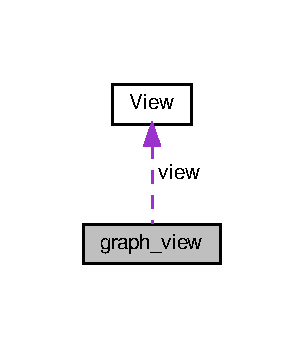
\includegraphics[width=146pt]{structgraph__view__coll__graph}
\end{center}
\end{figure}
\subsection*{Public Attributes}
\begin{DoxyCompactItemize}
\item 
\hyperlink{structView}{View} $\ast$ \hyperlink{structgraph__view_a44e9bb5000071005cad8bf8fe330ad45}{view}
\item 
unsigned char \hyperlink{structgraph__view_aea851ba75c3cf634c25aa11fcb08299c}{vertical\+\_\+tick\+\_\+marks}
\item 
unsigned char \hyperlink{structgraph__view_ac28c09dcb169d06d829dd6aed28f8685}{horizontal\+\_\+tick\+\_\+marks}
\end{DoxyCompactItemize}


\subsection{Member Data Documentation}
\mbox{\Hypertarget{structgraph__view_ac28c09dcb169d06d829dd6aed28f8685}\label{structgraph__view_ac28c09dcb169d06d829dd6aed28f8685}} 
\index{graph\+\_\+view@{graph\+\_\+view}!horizontal\+\_\+tick\+\_\+marks@{horizontal\+\_\+tick\+\_\+marks}}
\index{horizontal\+\_\+tick\+\_\+marks@{horizontal\+\_\+tick\+\_\+marks}!graph\+\_\+view@{graph\+\_\+view}}
\subsubsection{\texorpdfstring{horizontal\+\_\+tick\+\_\+marks}{horizontal\_tick\_marks}}
{\footnotesize\ttfamily unsigned char graph\+\_\+view\+::horizontal\+\_\+tick\+\_\+marks}

\mbox{\Hypertarget{structgraph__view_aea851ba75c3cf634c25aa11fcb08299c}\label{structgraph__view_aea851ba75c3cf634c25aa11fcb08299c}} 
\index{graph\+\_\+view@{graph\+\_\+view}!vertical\+\_\+tick\+\_\+marks@{vertical\+\_\+tick\+\_\+marks}}
\index{vertical\+\_\+tick\+\_\+marks@{vertical\+\_\+tick\+\_\+marks}!graph\+\_\+view@{graph\+\_\+view}}
\subsubsection{\texorpdfstring{vertical\+\_\+tick\+\_\+marks}{vertical\_tick\_marks}}
{\footnotesize\ttfamily unsigned char graph\+\_\+view\+::vertical\+\_\+tick\+\_\+marks}

\mbox{\Hypertarget{structgraph__view_a44e9bb5000071005cad8bf8fe330ad45}\label{structgraph__view_a44e9bb5000071005cad8bf8fe330ad45}} 
\index{graph\+\_\+view@{graph\+\_\+view}!view@{view}}
\index{view@{view}!graph\+\_\+view@{graph\+\_\+view}}
\subsubsection{\texorpdfstring{view}{view}}
{\footnotesize\ttfamily \hyperlink{structView}{View}$\ast$ graph\+\_\+view\+::view}



The documentation for this struct was generated from the following file\+:\begin{DoxyCompactItemize}
\item 
\hyperlink{graphics_8h}{graphics.\+h}\end{DoxyCompactItemize}

\hypertarget{structHashmap}{}\section{Hashmap Struct Reference}
\label{structHashmap}\index{Hashmap@{Hashmap}}


{\ttfamily \#include $<$hashmap.\+h$>$}



Collaboration diagram for Hashmap\+:\nopagebreak
\begin{figure}[H]
\begin{center}
\leavevmode
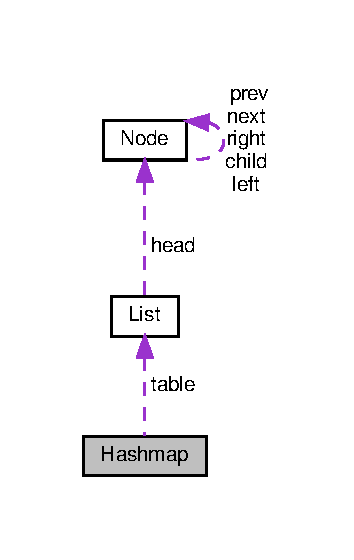
\includegraphics[width=170pt]{structHashmap__coll__graph}
\end{center}
\end{figure}
\subsection*{Public Attributes}
\begin{DoxyCompactItemize}
\item 
unsigned int \hyperlink{structHashmap_acf25511ea4f01ef33fa00e3b40fddfb8}{elements}
\item 
unsigned int \hyperlink{structHashmap_acb5951c2662ce58e2196fcb465551e36}{size}
\item 
\hyperlink{structList}{List} $\ast$$\ast$ \hyperlink{structHashmap_a84d20ef62c1f397de5fdac234445c1e7}{table}
\item 
void $\ast$($\ast$ \hyperlink{structHashmap_a94750a8d94eb1d30ad153ccc447c40ae}{get} )(\hyperlink{structHashmap}{Hashmap} $\ast$this, char $\ast$string)
\item 
void($\ast$ \hyperlink{structHashmap_a86fd2c2aaa8f266c2e99a035479b67df}{add} )(\hyperlink{structHashmap}{Hashmap} $\ast$this, char $\ast$string, void $\ast$datum)
\item 
void($\ast$ \hyperlink{structHashmap_a869ddf80d753042c35a4741a0bd5b10b}{remove} )(\hyperlink{structHashmap}{Hashmap} $\ast$this, char $\ast$string)
\item 
bool($\ast$ \hyperlink{structHashmap_abcabe76ebc3b3f7744bc78b3d31682dc}{exists} )(\hyperlink{structHashmap}{Hashmap} $\ast$this, char $\ast$string)
\item 
void($\ast$ \hyperlink{structHashmap_ac7249166e6305fcec9a7fd4be614c3cd}{update} )(\hyperlink{structHashmap}{Hashmap} $\ast$this, char $\ast$string, void $\ast$datum)
\end{DoxyCompactItemize}


\subsection{Member Data Documentation}
\mbox{\Hypertarget{structHashmap_a86fd2c2aaa8f266c2e99a035479b67df}\label{structHashmap_a86fd2c2aaa8f266c2e99a035479b67df}} 
\index{Hashmap@{Hashmap}!add@{add}}
\index{add@{add}!Hashmap@{Hashmap}}
\subsubsection{\texorpdfstring{add}{add}}
{\footnotesize\ttfamily void($\ast$  Hashmap\+::add) (\hyperlink{structHashmap}{Hashmap} $\ast$this, char $\ast$string, void $\ast$datum)}

\mbox{\Hypertarget{structHashmap_acf25511ea4f01ef33fa00e3b40fddfb8}\label{structHashmap_acf25511ea4f01ef33fa00e3b40fddfb8}} 
\index{Hashmap@{Hashmap}!elements@{elements}}
\index{elements@{elements}!Hashmap@{Hashmap}}
\subsubsection{\texorpdfstring{elements}{elements}}
{\footnotesize\ttfamily unsigned int Hashmap\+::elements}

\mbox{\Hypertarget{structHashmap_abcabe76ebc3b3f7744bc78b3d31682dc}\label{structHashmap_abcabe76ebc3b3f7744bc78b3d31682dc}} 
\index{Hashmap@{Hashmap}!exists@{exists}}
\index{exists@{exists}!Hashmap@{Hashmap}}
\subsubsection{\texorpdfstring{exists}{exists}}
{\footnotesize\ttfamily bool($\ast$  Hashmap\+::exists) (\hyperlink{structHashmap}{Hashmap} $\ast$this, char $\ast$string)}

\mbox{\Hypertarget{structHashmap_a94750a8d94eb1d30ad153ccc447c40ae}\label{structHashmap_a94750a8d94eb1d30ad153ccc447c40ae}} 
\index{Hashmap@{Hashmap}!get@{get}}
\index{get@{get}!Hashmap@{Hashmap}}
\subsubsection{\texorpdfstring{get}{get}}
{\footnotesize\ttfamily void$\ast$($\ast$  Hashmap\+::get) (\hyperlink{structHashmap}{Hashmap} $\ast$this, char $\ast$string)}

\mbox{\Hypertarget{structHashmap_a869ddf80d753042c35a4741a0bd5b10b}\label{structHashmap_a869ddf80d753042c35a4741a0bd5b10b}} 
\index{Hashmap@{Hashmap}!remove@{remove}}
\index{remove@{remove}!Hashmap@{Hashmap}}
\subsubsection{\texorpdfstring{remove}{remove}}
{\footnotesize\ttfamily void($\ast$  Hashmap\+::remove) (\hyperlink{structHashmap}{Hashmap} $\ast$this, char $\ast$string)}

\mbox{\Hypertarget{structHashmap_acb5951c2662ce58e2196fcb465551e36}\label{structHashmap_acb5951c2662ce58e2196fcb465551e36}} 
\index{Hashmap@{Hashmap}!size@{size}}
\index{size@{size}!Hashmap@{Hashmap}}
\subsubsection{\texorpdfstring{size}{size}}
{\footnotesize\ttfamily unsigned int Hashmap\+::size}

\mbox{\Hypertarget{structHashmap_a84d20ef62c1f397de5fdac234445c1e7}\label{structHashmap_a84d20ef62c1f397de5fdac234445c1e7}} 
\index{Hashmap@{Hashmap}!table@{table}}
\index{table@{table}!Hashmap@{Hashmap}}
\subsubsection{\texorpdfstring{table}{table}}
{\footnotesize\ttfamily \hyperlink{structList}{List}$\ast$$\ast$ Hashmap\+::table}

\mbox{\Hypertarget{structHashmap_ac7249166e6305fcec9a7fd4be614c3cd}\label{structHashmap_ac7249166e6305fcec9a7fd4be614c3cd}} 
\index{Hashmap@{Hashmap}!update@{update}}
\index{update@{update}!Hashmap@{Hashmap}}
\subsubsection{\texorpdfstring{update}{update}}
{\footnotesize\ttfamily void($\ast$  Hashmap\+::update) (\hyperlink{structHashmap}{Hashmap} $\ast$this, char $\ast$string, void $\ast$datum)}



The documentation for this struct was generated from the following file\+:\begin{DoxyCompactItemize}
\item 
\hyperlink{hashmap_8h}{hashmap.\+h}\end{DoxyCompactItemize}

\hypertarget{structHashmapElement}{}\section{Hashmap\+Element Struct Reference}
\label{structHashmapElement}\index{Hashmap\+Element@{Hashmap\+Element}}


{\ttfamily \#include $<$hashmap.\+h$>$}

\subsection*{Public Attributes}
\begin{DoxyCompactItemize}
\item 
char $\ast$ \hyperlink{structHashmapElement_a14c854540e557b6e3f78e5b2229fb694}{key}
\item 
void $\ast$ \hyperlink{structHashmapElement_a0aa5a85cb3645771dad624aa385db83e}{datum}
\end{DoxyCompactItemize}


\subsection{Member Data Documentation}
\mbox{\Hypertarget{structHashmapElement_a0aa5a85cb3645771dad624aa385db83e}\label{structHashmapElement_a0aa5a85cb3645771dad624aa385db83e}} 
\index{Hashmap\+Element@{Hashmap\+Element}!datum@{datum}}
\index{datum@{datum}!Hashmap\+Element@{Hashmap\+Element}}
\subsubsection{\texorpdfstring{datum}{datum}}
{\footnotesize\ttfamily void$\ast$ Hashmap\+Element\+::datum}

\mbox{\Hypertarget{structHashmapElement_a14c854540e557b6e3f78e5b2229fb694}\label{structHashmapElement_a14c854540e557b6e3f78e5b2229fb694}} 
\index{Hashmap\+Element@{Hashmap\+Element}!key@{key}}
\index{key@{key}!Hashmap\+Element@{Hashmap\+Element}}
\subsubsection{\texorpdfstring{key}{key}}
{\footnotesize\ttfamily char$\ast$ Hashmap\+Element\+::key}



The documentation for this struct was generated from the following file\+:\begin{DoxyCompactItemize}
\item 
\hyperlink{hashmap_8h}{hashmap.\+h}\end{DoxyCompactItemize}

\hypertarget{structI2C}{}\section{I2C Struct Reference}
\label{structI2C}\index{I2C@{I2C}}


{\ttfamily \#include $<$i2c-\/interface.\+h$>$}

\subsection*{Public Attributes}
\begin{DoxyCompactItemize}
\item 
unsigned char \hyperlink{structI2C_a2cb6b6925aa9cf1d5f878b33d176df26}{i2c\+\_\+address}
\item 
unsigned char \hyperlink{structI2C_a2f9f539ab4ca498f89fb6e95334d0354}{i2c\+\_\+slave\+\_\+address}
\item 
short $\ast$ \hyperlink{structI2C_a0bf74755f449fe6216c70bea75367332}{registers}
\item 
void($\ast$ \hyperlink{structI2C_a057e451794e3497ac6a0daa29d89fa49}{gyros} )(float $\ast$axes)
\item 
void($\ast$ \hyperlink{structI2C_a364b791b69beaa2ef1111d8ec5565c6a}{accelerometers} )(float $\ast$axes)
\item 
void($\ast$ \hyperlink{structI2C_a1d9c6b23b7f65aeeb371e56134e90472}{magnetometers} )(float $\ast$axes)
\item 
float($\ast$ \hyperlink{structI2C_ad0c119ae909b7d0e608abc3a48910ce2}{temperature} )()
\end{DoxyCompactItemize}


\subsection{Member Data Documentation}
\mbox{\Hypertarget{structI2C_a364b791b69beaa2ef1111d8ec5565c6a}\label{structI2C_a364b791b69beaa2ef1111d8ec5565c6a}} 
\index{I2C@{I2C}!accelerometers@{accelerometers}}
\index{accelerometers@{accelerometers}!I2C@{I2C}}
\subsubsection{\texorpdfstring{accelerometers}{accelerometers}}
{\footnotesize\ttfamily void($\ast$  I2\+C\+::accelerometers) (float $\ast$axes)}

\mbox{\Hypertarget{structI2C_a057e451794e3497ac6a0daa29d89fa49}\label{structI2C_a057e451794e3497ac6a0daa29d89fa49}} 
\index{I2C@{I2C}!gyros@{gyros}}
\index{gyros@{gyros}!I2C@{I2C}}
\subsubsection{\texorpdfstring{gyros}{gyros}}
{\footnotesize\ttfamily void($\ast$  I2\+C\+::gyros) (float $\ast$axes)}

\mbox{\Hypertarget{structI2C_a2cb6b6925aa9cf1d5f878b33d176df26}\label{structI2C_a2cb6b6925aa9cf1d5f878b33d176df26}} 
\index{I2C@{I2C}!i2c\+\_\+address@{i2c\+\_\+address}}
\index{i2c\+\_\+address@{i2c\+\_\+address}!I2C@{I2C}}
\subsubsection{\texorpdfstring{i2c\+\_\+address}{i2c\_address}}
{\footnotesize\ttfamily unsigned char I2\+C\+::i2c\+\_\+address}

\mbox{\Hypertarget{structI2C_a2f9f539ab4ca498f89fb6e95334d0354}\label{structI2C_a2f9f539ab4ca498f89fb6e95334d0354}} 
\index{I2C@{I2C}!i2c\+\_\+slave\+\_\+address@{i2c\+\_\+slave\+\_\+address}}
\index{i2c\+\_\+slave\+\_\+address@{i2c\+\_\+slave\+\_\+address}!I2C@{I2C}}
\subsubsection{\texorpdfstring{i2c\+\_\+slave\+\_\+address}{i2c\_slave\_address}}
{\footnotesize\ttfamily unsigned char I2\+C\+::i2c\+\_\+slave\+\_\+address}

\mbox{\Hypertarget{structI2C_a1d9c6b23b7f65aeeb371e56134e90472}\label{structI2C_a1d9c6b23b7f65aeeb371e56134e90472}} 
\index{I2C@{I2C}!magnetometers@{magnetometers}}
\index{magnetometers@{magnetometers}!I2C@{I2C}}
\subsubsection{\texorpdfstring{magnetometers}{magnetometers}}
{\footnotesize\ttfamily void($\ast$  I2\+C\+::magnetometers) (float $\ast$axes)}

\mbox{\Hypertarget{structI2C_a0bf74755f449fe6216c70bea75367332}\label{structI2C_a0bf74755f449fe6216c70bea75367332}} 
\index{I2C@{I2C}!registers@{registers}}
\index{registers@{registers}!I2C@{I2C}}
\subsubsection{\texorpdfstring{registers}{registers}}
{\footnotesize\ttfamily short$\ast$ I2\+C\+::registers}

\mbox{\Hypertarget{structI2C_ad0c119ae909b7d0e608abc3a48910ce2}\label{structI2C_ad0c119ae909b7d0e608abc3a48910ce2}} 
\index{I2C@{I2C}!temperature@{temperature}}
\index{temperature@{temperature}!I2C@{I2C}}
\subsubsection{\texorpdfstring{temperature}{temperature}}
{\footnotesize\ttfamily float($\ast$  I2\+C\+::temperature) ()}



The documentation for this struct was generated from the following file\+:\begin{DoxyCompactItemize}
\item 
\hyperlink{i2c-interface_8h}{i2c-\/interface.\+h}\end{DoxyCompactItemize}

\hypertarget{structList}{}\section{List Struct Reference}
\label{structList}\index{List@{List}}


{\ttfamily \#include $<$linked-\/list.\+h$>$}



Collaboration diagram for List\+:
\nopagebreak
\begin{figure}[H]
\begin{center}
\leavevmode
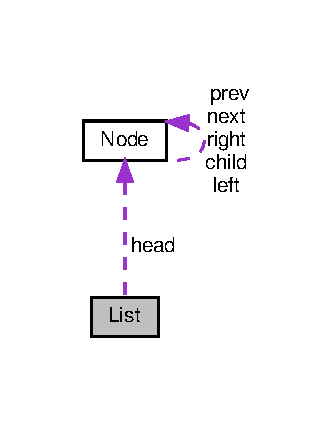
\includegraphics[width=160pt]{structList__coll__graph}
\end{center}
\end{figure}
\subsection*{Public Attributes}
\begin{DoxyCompactItemize}
\item 
\hyperlink{structNode}{Node} $\ast$ \hyperlink{structList_a443db628080a04a1dacfd3015d164735}{head}
\item 
unsigned int \hyperlink{structList_a388b6c8fff13e506d27071a318c9004f}{elements}
\item 
unsigned int \hyperlink{structList_a3858093f64846444abc72e9b31e00e41}{elements\+\_\+limit}
\item 
bool \hyperlink{structList_a0a6b9ea561ca0cff5c3e7673717676c2}{doublely\+\_\+linked}
\end{DoxyCompactItemize}


\subsection{Member Data Documentation}
\mbox{\Hypertarget{structList_a0a6b9ea561ca0cff5c3e7673717676c2}\label{structList_a0a6b9ea561ca0cff5c3e7673717676c2}} 
\index{List@{List}!doublely\+\_\+linked@{doublely\+\_\+linked}}
\index{doublely\+\_\+linked@{doublely\+\_\+linked}!List@{List}}
\subsubsection{\texorpdfstring{doublely\+\_\+linked}{doublely\_linked}}
{\footnotesize\ttfamily bool List\+::doublely\+\_\+linked}

\mbox{\Hypertarget{structList_a388b6c8fff13e506d27071a318c9004f}\label{structList_a388b6c8fff13e506d27071a318c9004f}} 
\index{List@{List}!elements@{elements}}
\index{elements@{elements}!List@{List}}
\subsubsection{\texorpdfstring{elements}{elements}}
{\footnotesize\ttfamily unsigned int List\+::elements}

\mbox{\Hypertarget{structList_a3858093f64846444abc72e9b31e00e41}\label{structList_a3858093f64846444abc72e9b31e00e41}} 
\index{List@{List}!elements\+\_\+limit@{elements\+\_\+limit}}
\index{elements\+\_\+limit@{elements\+\_\+limit}!List@{List}}
\subsubsection{\texorpdfstring{elements\+\_\+limit}{elements\_limit}}
{\footnotesize\ttfamily unsigned int List\+::elements\+\_\+limit}

\mbox{\Hypertarget{structList_a443db628080a04a1dacfd3015d164735}\label{structList_a443db628080a04a1dacfd3015d164735}} 
\index{List@{List}!head@{head}}
\index{head@{head}!List@{List}}
\subsubsection{\texorpdfstring{head}{head}}
{\footnotesize\ttfamily \hyperlink{structNode}{Node}$\ast$ List\+::head}



The documentation for this struct was generated from the following file\+:\begin{DoxyCompactItemize}
\item 
\hyperlink{linked-list_8h}{linked-\/list.\+h}\end{DoxyCompactItemize}

\hypertarget{structLogger}{}\section{Logger Struct Reference}
\label{structLogger}\index{Logger@{Logger}}


{\ttfamily \#include $<$logger.\+h$>$}



Collaboration diagram for Logger\+:\nopagebreak
\begin{figure}[H]
\begin{center}
\leavevmode
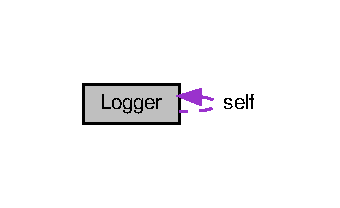
\includegraphics[width=163pt]{structLogger__coll__graph}
\end{center}
\end{figure}
\subsection*{Public Attributes}
\begin{DoxyCompactItemize}
\item 
\hyperlink{structLogger}{Logger} $\ast$ \hyperlink{structLogger_a220cd94b89be365dba07df9cbdf2d15f}{self}
\item 
F\+I\+LE $\ast$ \hyperlink{structLogger_ad00c914c1f38de6d069cb788b9074d8f}{file}
\item 
char $\ast$ \hyperlink{structLogger_a4a7913dbecc583e935e8c18ec62716ab}{filename}
\item 
pthread\+\_\+t \hyperlink{structLogger_a69e132f8b832286f2bfd777d0a6bc266}{thread}
\item 
bool \hyperlink{structLogger_af3c673bf2d3f729549722c0beab4f34c}{termination\+\_\+signal}
\item 
int \hyperlink{structLogger_aa5a4930df402c7b25487a1315b9a94f4}{values\+\_\+read}
\item 
bool($\ast$ \hyperlink{structLogger_a8b371035a67cc1da7cd1c0d0ae5dd69d}{open} )(\hyperlink{structLogger}{Logger} $\ast$\hyperlink{structLogger_a220cd94b89be365dba07df9cbdf2d15f}{self})
\item 
bool($\ast$ \hyperlink{structLogger_a13192d1a123f8373bc8f9d680c8a8528}{close} )(\hyperlink{structLogger}{Logger} $\ast$\hyperlink{structLogger_a220cd94b89be365dba07df9cbdf2d15f}{self})
\item 
void($\ast$ \hyperlink{structLogger_ab665b6bcc0afa850994e8ad4cc4e6c4f}{destroy} )(\hyperlink{structLogger}{Logger} $\ast$\hyperlink{structLogger_a220cd94b89be365dba07df9cbdf2d15f}{self})
\end{DoxyCompactItemize}


\subsection{Member Data Documentation}
\mbox{\Hypertarget{structLogger_a13192d1a123f8373bc8f9d680c8a8528}\label{structLogger_a13192d1a123f8373bc8f9d680c8a8528}} 
\index{Logger@{Logger}!close@{close}}
\index{close@{close}!Logger@{Logger}}
\subsubsection{\texorpdfstring{close}{close}}
{\footnotesize\ttfamily bool($\ast$  Logger\+::close) (\hyperlink{structLogger}{Logger} $\ast$\hyperlink{structLogger_a220cd94b89be365dba07df9cbdf2d15f}{self})}

\mbox{\Hypertarget{structLogger_ab665b6bcc0afa850994e8ad4cc4e6c4f}\label{structLogger_ab665b6bcc0afa850994e8ad4cc4e6c4f}} 
\index{Logger@{Logger}!destroy@{destroy}}
\index{destroy@{destroy}!Logger@{Logger}}
\subsubsection{\texorpdfstring{destroy}{destroy}}
{\footnotesize\ttfamily void($\ast$  Logger\+::destroy) (\hyperlink{structLogger}{Logger} $\ast$\hyperlink{structLogger_a220cd94b89be365dba07df9cbdf2d15f}{self})}

\mbox{\Hypertarget{structLogger_ad00c914c1f38de6d069cb788b9074d8f}\label{structLogger_ad00c914c1f38de6d069cb788b9074d8f}} 
\index{Logger@{Logger}!file@{file}}
\index{file@{file}!Logger@{Logger}}
\subsubsection{\texorpdfstring{file}{file}}
{\footnotesize\ttfamily F\+I\+LE$\ast$ Logger\+::file}

\mbox{\Hypertarget{structLogger_a4a7913dbecc583e935e8c18ec62716ab}\label{structLogger_a4a7913dbecc583e935e8c18ec62716ab}} 
\index{Logger@{Logger}!filename@{filename}}
\index{filename@{filename}!Logger@{Logger}}
\subsubsection{\texorpdfstring{filename}{filename}}
{\footnotesize\ttfamily char$\ast$ Logger\+::filename}

\mbox{\Hypertarget{structLogger_a8b371035a67cc1da7cd1c0d0ae5dd69d}\label{structLogger_a8b371035a67cc1da7cd1c0d0ae5dd69d}} 
\index{Logger@{Logger}!open@{open}}
\index{open@{open}!Logger@{Logger}}
\subsubsection{\texorpdfstring{open}{open}}
{\footnotesize\ttfamily bool($\ast$  Logger\+::open) (\hyperlink{structLogger}{Logger} $\ast$\hyperlink{structLogger_a220cd94b89be365dba07df9cbdf2d15f}{self})}

\mbox{\Hypertarget{structLogger_a220cd94b89be365dba07df9cbdf2d15f}\label{structLogger_a220cd94b89be365dba07df9cbdf2d15f}} 
\index{Logger@{Logger}!self@{self}}
\index{self@{self}!Logger@{Logger}}
\subsubsection{\texorpdfstring{self}{self}}
{\footnotesize\ttfamily \hyperlink{structLogger}{Logger}$\ast$ Logger\+::self}

\mbox{\Hypertarget{structLogger_af3c673bf2d3f729549722c0beab4f34c}\label{structLogger_af3c673bf2d3f729549722c0beab4f34c}} 
\index{Logger@{Logger}!termination\+\_\+signal@{termination\+\_\+signal}}
\index{termination\+\_\+signal@{termination\+\_\+signal}!Logger@{Logger}}
\subsubsection{\texorpdfstring{termination\+\_\+signal}{termination\_signal}}
{\footnotesize\ttfamily bool Logger\+::termination\+\_\+signal}

\mbox{\Hypertarget{structLogger_a69e132f8b832286f2bfd777d0a6bc266}\label{structLogger_a69e132f8b832286f2bfd777d0a6bc266}} 
\index{Logger@{Logger}!thread@{thread}}
\index{thread@{thread}!Logger@{Logger}}
\subsubsection{\texorpdfstring{thread}{thread}}
{\footnotesize\ttfamily pthread\+\_\+t Logger\+::thread}

\mbox{\Hypertarget{structLogger_aa5a4930df402c7b25487a1315b9a94f4}\label{structLogger_aa5a4930df402c7b25487a1315b9a94f4}} 
\index{Logger@{Logger}!values\+\_\+read@{values\+\_\+read}}
\index{values\+\_\+read@{values\+\_\+read}!Logger@{Logger}}
\subsubsection{\texorpdfstring{values\+\_\+read}{values\_read}}
{\footnotesize\ttfamily int Logger\+::values\+\_\+read}



The documentation for this struct was generated from the following file\+:\begin{DoxyCompactItemize}
\item 
\hyperlink{logger_8h}{logger.\+h}\end{DoxyCompactItemize}

\hypertarget{structmodule}{}\section{module Struct Reference}
\label{structmodule}\index{module@{module}}


{\ttfamily \#include $<$femta.\+h$>$}



Collaboration diagram for module\+:\nopagebreak
\begin{figure}[H]
\begin{center}
\leavevmode
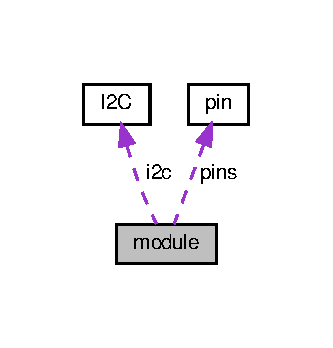
\includegraphics[width=160pt]{structmodule__coll__graph}
\end{center}
\end{figure}
\subsection*{Public Attributes}
\begin{DoxyCompactItemize}
\item 
char $\ast$ \hyperlink{structmodule_ab82c1bea579b33b2855bd99cc6277c8a}{identifier}
\item 
\hyperlink{structpin}{pin} $\ast$ \hyperlink{structmodule_a3a758f16bbf56b5df5bfb1cfd7515fdb}{pins}
\item 
char \hyperlink{structmodule_a02c9f82d64608b57e23ec9b6d8e40442}{n\+\_\+pins}
\item 
\hyperlink{structI2C}{I2C} $\ast$ \hyperlink{structmodule_aedc78b570290808d3e47d2bb2dadd155}{i2c}
\item 
\hyperlink{femta_8h_a13b3221f36ef9cb93c995303f10fed50}{U\+A\+RT} $\ast$ \hyperlink{structmodule_af74c4f29b898b255838d6b18731fa565}{uart}
\item 
bool \hyperlink{structmodule_a9b7ebb7008b8bc642090447151895cae}{initialized}
\item 
bool \hyperlink{structmodule_a321b33f91b9b132f34d66fef4243e201}{loaded}
\item 
bool \hyperlink{structmodule_ac6281658345d8c0ebd189f10feca7f8c}{enabled}
\end{DoxyCompactItemize}


\subsection{Member Data Documentation}
\mbox{\Hypertarget{structmodule_ac6281658345d8c0ebd189f10feca7f8c}\label{structmodule_ac6281658345d8c0ebd189f10feca7f8c}} 
\index{module@{module}!enabled@{enabled}}
\index{enabled@{enabled}!module@{module}}
\subsubsection{\texorpdfstring{enabled}{enabled}}
{\footnotesize\ttfamily bool module\+::enabled}

\mbox{\Hypertarget{structmodule_aedc78b570290808d3e47d2bb2dadd155}\label{structmodule_aedc78b570290808d3e47d2bb2dadd155}} 
\index{module@{module}!i2c@{i2c}}
\index{i2c@{i2c}!module@{module}}
\subsubsection{\texorpdfstring{i2c}{i2c}}
{\footnotesize\ttfamily \hyperlink{structI2C}{I2C}$\ast$ module\+::i2c}

\mbox{\Hypertarget{structmodule_ab82c1bea579b33b2855bd99cc6277c8a}\label{structmodule_ab82c1bea579b33b2855bd99cc6277c8a}} 
\index{module@{module}!identifier@{identifier}}
\index{identifier@{identifier}!module@{module}}
\subsubsection{\texorpdfstring{identifier}{identifier}}
{\footnotesize\ttfamily char$\ast$ module\+::identifier}

\mbox{\Hypertarget{structmodule_a9b7ebb7008b8bc642090447151895cae}\label{structmodule_a9b7ebb7008b8bc642090447151895cae}} 
\index{module@{module}!initialized@{initialized}}
\index{initialized@{initialized}!module@{module}}
\subsubsection{\texorpdfstring{initialized}{initialized}}
{\footnotesize\ttfamily bool module\+::initialized}

\mbox{\Hypertarget{structmodule_a321b33f91b9b132f34d66fef4243e201}\label{structmodule_a321b33f91b9b132f34d66fef4243e201}} 
\index{module@{module}!loaded@{loaded}}
\index{loaded@{loaded}!module@{module}}
\subsubsection{\texorpdfstring{loaded}{loaded}}
{\footnotesize\ttfamily bool module\+::loaded}

\mbox{\Hypertarget{structmodule_a02c9f82d64608b57e23ec9b6d8e40442}\label{structmodule_a02c9f82d64608b57e23ec9b6d8e40442}} 
\index{module@{module}!n\+\_\+pins@{n\+\_\+pins}}
\index{n\+\_\+pins@{n\+\_\+pins}!module@{module}}
\subsubsection{\texorpdfstring{n\+\_\+pins}{n\_pins}}
{\footnotesize\ttfamily char module\+::n\+\_\+pins}

\mbox{\Hypertarget{structmodule_a3a758f16bbf56b5df5bfb1cfd7515fdb}\label{structmodule_a3a758f16bbf56b5df5bfb1cfd7515fdb}} 
\index{module@{module}!pins@{pins}}
\index{pins@{pins}!module@{module}}
\subsubsection{\texorpdfstring{pins}{pins}}
{\footnotesize\ttfamily \hyperlink{structpin}{pin}$\ast$ module\+::pins}

\mbox{\Hypertarget{structmodule_af74c4f29b898b255838d6b18731fa565}\label{structmodule_af74c4f29b898b255838d6b18731fa565}} 
\index{module@{module}!uart@{uart}}
\index{uart@{uart}!module@{module}}
\subsubsection{\texorpdfstring{uart}{uart}}
{\footnotesize\ttfamily \hyperlink{femta_8h_a13b3221f36ef9cb93c995303f10fed50}{U\+A\+RT}$\ast$ module\+::uart}



The documentation for this struct was generated from the following file\+:\begin{DoxyCompactItemize}
\item 
\hyperlink{femta_8h}{femta.\+h}\end{DoxyCompactItemize}

\hypertarget{structNode}{}\section{Node Struct Reference}
\label{structNode}\index{Node@{Node}}


{\ttfamily \#include $<$linked-\/list.\+h$>$}



Collaboration diagram for Node\+:
\nopagebreak
\begin{figure}[H]
\begin{center}
\leavevmode
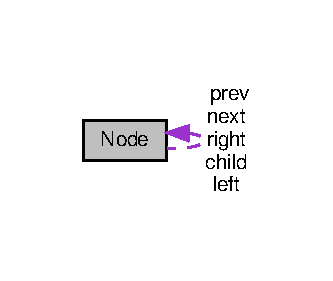
\includegraphics[width=160pt]{structNode__coll__graph}
\end{center}
\end{figure}
\subsection*{Public Attributes}
\begin{DoxyCompactItemize}
\item 
\begin{tabbing}
xx\=xx\=xx\=xx\=xx\=xx\=xx\=xx\=xx\=\kill
union \{\\
\>\hyperlink{structNode}{Node} $\ast$ \hyperlink{structNode_a2559a716f69ccaa76d648d9f1b83065e}{next}\\
\>\hyperlink{structNode}{Node} $\ast$ \hyperlink{structNode_a7328862eaa6dea28018326549b3294d3}{right}\\
\}; \\

\end{tabbing}\item 
\begin{tabbing}
xx\=xx\=xx\=xx\=xx\=xx\=xx\=xx\=xx\=\kill
union \{\\
\>\hyperlink{structNode}{Node} $\ast$ \hyperlink{structNode_a632ea91c6a13082308f7692649a68880}{prev}\\
\>\hyperlink{structNode}{Node} $\ast$ \hyperlink{structNode_ab8c667ac8fdb120ed4c031682a9cdaee}{left}\\
\>\hyperlink{structNode}{Node} $\ast$ \hyperlink{structNode_ad55e191b2855879d7b761258d64e2667}{child}\\
\}; \\

\end{tabbing}\item 
void $\ast$ \hyperlink{structNode_a520bf86af21ca233eb9f58e9e28c6576}{value}
\end{DoxyCompactItemize}


\subsection{Member Data Documentation}
\mbox{\Hypertarget{structNode_a54ef89ca60997c37464b33e2bc1fa520}\label{structNode_a54ef89ca60997c37464b33e2bc1fa520}} 
\subsubsection{\texorpdfstring{"@3}{@3}}
{\footnotesize\ttfamily union \{ ... \} }

\mbox{\Hypertarget{structNode_a6be5b0f6c9a9396734c0e7cd97b35a85}\label{structNode_a6be5b0f6c9a9396734c0e7cd97b35a85}} 
\subsubsection{\texorpdfstring{"@5}{@5}}
{\footnotesize\ttfamily union \{ ... \} }

\mbox{\Hypertarget{structNode_ad55e191b2855879d7b761258d64e2667}\label{structNode_ad55e191b2855879d7b761258d64e2667}} 
\index{Node@{Node}!child@{child}}
\index{child@{child}!Node@{Node}}
\subsubsection{\texorpdfstring{child}{child}}
{\footnotesize\ttfamily \hyperlink{structNode}{Node}$\ast$ Node\+::child}

\mbox{\Hypertarget{structNode_ab8c667ac8fdb120ed4c031682a9cdaee}\label{structNode_ab8c667ac8fdb120ed4c031682a9cdaee}} 
\index{Node@{Node}!left@{left}}
\index{left@{left}!Node@{Node}}
\subsubsection{\texorpdfstring{left}{left}}
{\footnotesize\ttfamily \hyperlink{structNode}{Node}$\ast$ Node\+::left}

\mbox{\Hypertarget{structNode_a2559a716f69ccaa76d648d9f1b83065e}\label{structNode_a2559a716f69ccaa76d648d9f1b83065e}} 
\index{Node@{Node}!next@{next}}
\index{next@{next}!Node@{Node}}
\subsubsection{\texorpdfstring{next}{next}}
{\footnotesize\ttfamily \hyperlink{structNode}{Node}$\ast$ Node\+::next}

\mbox{\Hypertarget{structNode_a632ea91c6a13082308f7692649a68880}\label{structNode_a632ea91c6a13082308f7692649a68880}} 
\index{Node@{Node}!prev@{prev}}
\index{prev@{prev}!Node@{Node}}
\subsubsection{\texorpdfstring{prev}{prev}}
{\footnotesize\ttfamily \hyperlink{structNode}{Node}$\ast$ Node\+::prev}

\mbox{\Hypertarget{structNode_a7328862eaa6dea28018326549b3294d3}\label{structNode_a7328862eaa6dea28018326549b3294d3}} 
\index{Node@{Node}!right@{right}}
\index{right@{right}!Node@{Node}}
\subsubsection{\texorpdfstring{right}{right}}
{\footnotesize\ttfamily \hyperlink{structNode}{Node}$\ast$ Node\+::right}

\mbox{\Hypertarget{structNode_a520bf86af21ca233eb9f58e9e28c6576}\label{structNode_a520bf86af21ca233eb9f58e9e28c6576}} 
\index{Node@{Node}!value@{value}}
\index{value@{value}!Node@{Node}}
\subsubsection{\texorpdfstring{value}{value}}
{\footnotesize\ttfamily void$\ast$ Node\+::value}



The documentation for this struct was generated from the following file\+:\begin{DoxyCompactItemize}
\item 
\hyperlink{linked-list_8h}{linked-\/list.\+h}\end{DoxyCompactItemize}

\hypertarget{structpin}{}\section{pin Struct Reference}
\label{structpin}\index{pin@{pin}}


{\ttfamily \#include $<$femta.\+h$>$}

\subsection*{Public Attributes}
\begin{DoxyCompactItemize}
\item 
char \hyperlink{structpin_a59c3020dc417fbda00ae4926db264a51}{state}
\item 
char \hyperlink{structpin_a5904e86c433f331ce55ed3ead575a802}{logical}
\item 
char \hyperlink{structpin_a0d3051114699672c833f272c06f2c658}{physical}
\item 
\begin{tabbing}
xx\=xx\=xx\=xx\=xx\=xx\=xx\=xx\=xx\=\kill
union \{\\
\>char \hyperlink{structpin_a11d53a2f512e95511a962537d333d9b5}{voltage}\\
\>unsigned char \hyperlink{structpin_a146ea977cbe36e19bd786615467a6106}{duty\_cycle}\\
\}; \\

\end{tabbing}\end{DoxyCompactItemize}


\subsection{Member Data Documentation}
\mbox{\Hypertarget{structpin_a5afcad2d92d6a6b92e9c58c02bdf8ce8}\label{structpin_a5afcad2d92d6a6b92e9c58c02bdf8ce8}} 
\subsubsection{\texorpdfstring{"@1}{@1}}
{\footnotesize\ttfamily union \{ ... \} }

\mbox{\Hypertarget{structpin_a146ea977cbe36e19bd786615467a6106}\label{structpin_a146ea977cbe36e19bd786615467a6106}} 
\index{pin@{pin}!duty\+\_\+cycle@{duty\+\_\+cycle}}
\index{duty\+\_\+cycle@{duty\+\_\+cycle}!pin@{pin}}
\subsubsection{\texorpdfstring{duty\+\_\+cycle}{duty\_cycle}}
{\footnotesize\ttfamily unsigned char pin\+::duty\+\_\+cycle}

\mbox{\Hypertarget{structpin_a5904e86c433f331ce55ed3ead575a802}\label{structpin_a5904e86c433f331ce55ed3ead575a802}} 
\index{pin@{pin}!logical@{logical}}
\index{logical@{logical}!pin@{pin}}
\subsubsection{\texorpdfstring{logical}{logical}}
{\footnotesize\ttfamily char pin\+::logical}

\mbox{\Hypertarget{structpin_a0d3051114699672c833f272c06f2c658}\label{structpin_a0d3051114699672c833f272c06f2c658}} 
\index{pin@{pin}!physical@{physical}}
\index{physical@{physical}!pin@{pin}}
\subsubsection{\texorpdfstring{physical}{physical}}
{\footnotesize\ttfamily char pin\+::physical}

\mbox{\Hypertarget{structpin_a59c3020dc417fbda00ae4926db264a51}\label{structpin_a59c3020dc417fbda00ae4926db264a51}} 
\index{pin@{pin}!state@{state}}
\index{state@{state}!pin@{pin}}
\subsubsection{\texorpdfstring{state}{state}}
{\footnotesize\ttfamily char pin\+::state}

\mbox{\Hypertarget{structpin_a11d53a2f512e95511a962537d333d9b5}\label{structpin_a11d53a2f512e95511a962537d333d9b5}} 
\index{pin@{pin}!voltage@{voltage}}
\index{voltage@{voltage}!pin@{pin}}
\subsubsection{\texorpdfstring{voltage}{voltage}}
{\footnotesize\ttfamily char pin\+::voltage}



The documentation for this struct was generated from the following file\+:\begin{DoxyCompactItemize}
\item 
\hyperlink{femta_8h}{femta.\+h}\end{DoxyCompactItemize}

\hypertarget{structPlot}{}\section{Plot Struct Reference}
\label{structPlot}\index{Plot@{Plot}}


{\ttfamily \#include $<$graphics.\+h$>$}



Collaboration diagram for Plot\+:\nopagebreak
\begin{figure}[H]
\begin{center}
\leavevmode
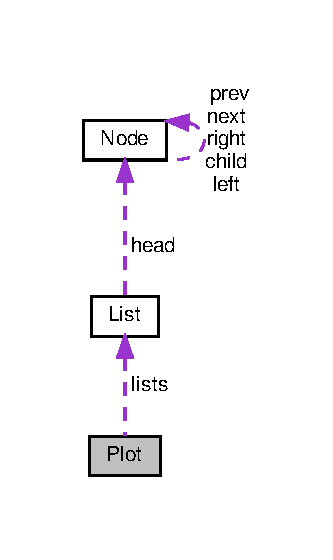
\includegraphics[width=160pt]{structPlot__coll__graph}
\end{center}
\end{figure}
\subsection*{Public Attributes}
\begin{DoxyCompactItemize}
\item 
char $\ast$ \hyperlink{structPlot_aa4c1f8e3360f2c41e22e041e1deba9b3}{name}
\item 
\hyperlink{structList}{List} $\ast$$\ast$ \hyperlink{structPlot_acf1191deb7d04e69106419aa87d3729d}{lists}
\item 
unsigned char \hyperlink{structPlot_ae7098880dbd6c20d2a1447fafea20e7b}{number\+\_\+of\+\_\+lists}
\item 
float \hyperlink{structPlot_a2fdd041a89c93f3b540ce57a59bce41c}{min\+\_\+value}
\item 
float \hyperlink{structPlot_ad174b1c447b62ea0e4a49fd3e324ddf0}{max\+\_\+value}
\item 
bool \hyperlink{structPlot_ab710f00d48f56ceb2c8d9345e6334e45}{has\+\_\+data}
\end{DoxyCompactItemize}


\subsection{Member Data Documentation}
\mbox{\Hypertarget{structPlot_ab710f00d48f56ceb2c8d9345e6334e45}\label{structPlot_ab710f00d48f56ceb2c8d9345e6334e45}} 
\index{Plot@{Plot}!has\+\_\+data@{has\+\_\+data}}
\index{has\+\_\+data@{has\+\_\+data}!Plot@{Plot}}
\subsubsection{\texorpdfstring{has\+\_\+data}{has\_data}}
{\footnotesize\ttfamily bool Plot\+::has\+\_\+data}

\mbox{\Hypertarget{structPlot_acf1191deb7d04e69106419aa87d3729d}\label{structPlot_acf1191deb7d04e69106419aa87d3729d}} 
\index{Plot@{Plot}!lists@{lists}}
\index{lists@{lists}!Plot@{Plot}}
\subsubsection{\texorpdfstring{lists}{lists}}
{\footnotesize\ttfamily \hyperlink{structList}{List}$\ast$$\ast$ Plot\+::lists}

\mbox{\Hypertarget{structPlot_ad174b1c447b62ea0e4a49fd3e324ddf0}\label{structPlot_ad174b1c447b62ea0e4a49fd3e324ddf0}} 
\index{Plot@{Plot}!max\+\_\+value@{max\+\_\+value}}
\index{max\+\_\+value@{max\+\_\+value}!Plot@{Plot}}
\subsubsection{\texorpdfstring{max\+\_\+value}{max\_value}}
{\footnotesize\ttfamily float Plot\+::max\+\_\+value}

\mbox{\Hypertarget{structPlot_a2fdd041a89c93f3b540ce57a59bce41c}\label{structPlot_a2fdd041a89c93f3b540ce57a59bce41c}} 
\index{Plot@{Plot}!min\+\_\+value@{min\+\_\+value}}
\index{min\+\_\+value@{min\+\_\+value}!Plot@{Plot}}
\subsubsection{\texorpdfstring{min\+\_\+value}{min\_value}}
{\footnotesize\ttfamily float Plot\+::min\+\_\+value}

\mbox{\Hypertarget{structPlot_aa4c1f8e3360f2c41e22e041e1deba9b3}\label{structPlot_aa4c1f8e3360f2c41e22e041e1deba9b3}} 
\index{Plot@{Plot}!name@{name}}
\index{name@{name}!Plot@{Plot}}
\subsubsection{\texorpdfstring{name}{name}}
{\footnotesize\ttfamily char$\ast$ Plot\+::name}

\mbox{\Hypertarget{structPlot_ae7098880dbd6c20d2a1447fafea20e7b}\label{structPlot_ae7098880dbd6c20d2a1447fafea20e7b}} 
\index{Plot@{Plot}!number\+\_\+of\+\_\+lists@{number\+\_\+of\+\_\+lists}}
\index{number\+\_\+of\+\_\+lists@{number\+\_\+of\+\_\+lists}!Plot@{Plot}}
\subsubsection{\texorpdfstring{number\+\_\+of\+\_\+lists}{number\_of\_lists}}
{\footnotesize\ttfamily unsigned char Plot\+::number\+\_\+of\+\_\+lists}



The documentation for this struct was generated from the following file\+:\begin{DoxyCompactItemize}
\item 
\hyperlink{graphics_8h}{graphics.\+h}\end{DoxyCompactItemize}

\hypertarget{structprint__view}{}\section{print\+\_\+view Struct Reference}
\label{structprint__view}\index{print\+\_\+view@{print\+\_\+view}}


{\ttfamily \#include $<$graphics.\+h$>$}



Collaboration diagram for print\+\_\+view\+:\nopagebreak
\begin{figure}[H]
\begin{center}
\leavevmode
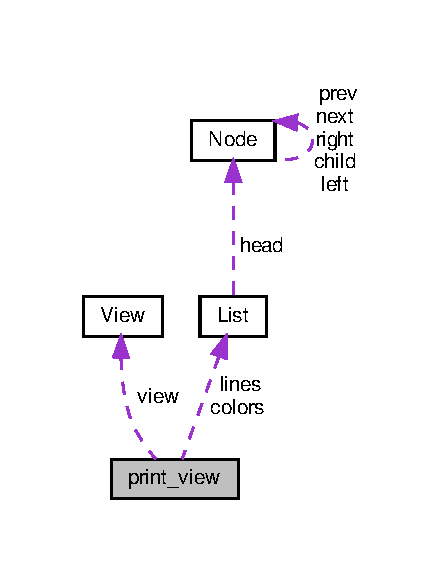
\includegraphics[width=212pt]{structprint__view__coll__graph}
\end{center}
\end{figure}
\subsection*{Public Attributes}
\begin{DoxyCompactItemize}
\item 
\hyperlink{structView}{View} $\ast$ \hyperlink{structprint__view_a189a4274f84ccdacb6210281d0163c7a}{view}
\item 
\hyperlink{structList}{List} $\ast$ \hyperlink{structprint__view_af78b98b8b676db7c0bf077cf1ac9aebb}{lines}
\item 
\hyperlink{structList}{List} $\ast$ \hyperlink{structprint__view_a58588dfd2ef043a6f042f10a295064e7}{colors}
\item 
unsigned char \hyperlink{structprint__view_a3a02430bd34dc873fc1cc61f7834d20e}{number\+\_\+lines\+\_\+printed}
\item 
unsigned char \hyperlink{structprint__view_ad5678744072375331613d2775773c933}{current\+\_\+view\+\_\+line}
\item 
unsigned char \hyperlink{structprint__view_a8f1ab6ae1c7d65a6535ce9cc3fa128b1}{number\+\_\+of\+\_\+lines}
\end{DoxyCompactItemize}


\subsection{Member Data Documentation}
\mbox{\Hypertarget{structprint__view_a58588dfd2ef043a6f042f10a295064e7}\label{structprint__view_a58588dfd2ef043a6f042f10a295064e7}} 
\index{print\+\_\+view@{print\+\_\+view}!colors@{colors}}
\index{colors@{colors}!print\+\_\+view@{print\+\_\+view}}
\subsubsection{\texorpdfstring{colors}{colors}}
{\footnotesize\ttfamily \hyperlink{structList}{List}$\ast$ print\+\_\+view\+::colors}

\mbox{\Hypertarget{structprint__view_ad5678744072375331613d2775773c933}\label{structprint__view_ad5678744072375331613d2775773c933}} 
\index{print\+\_\+view@{print\+\_\+view}!current\+\_\+view\+\_\+line@{current\+\_\+view\+\_\+line}}
\index{current\+\_\+view\+\_\+line@{current\+\_\+view\+\_\+line}!print\+\_\+view@{print\+\_\+view}}
\subsubsection{\texorpdfstring{current\+\_\+view\+\_\+line}{current\_view\_line}}
{\footnotesize\ttfamily unsigned char print\+\_\+view\+::current\+\_\+view\+\_\+line}

\mbox{\Hypertarget{structprint__view_af78b98b8b676db7c0bf077cf1ac9aebb}\label{structprint__view_af78b98b8b676db7c0bf077cf1ac9aebb}} 
\index{print\+\_\+view@{print\+\_\+view}!lines@{lines}}
\index{lines@{lines}!print\+\_\+view@{print\+\_\+view}}
\subsubsection{\texorpdfstring{lines}{lines}}
{\footnotesize\ttfamily \hyperlink{structList}{List}$\ast$ print\+\_\+view\+::lines}

\mbox{\Hypertarget{structprint__view_a3a02430bd34dc873fc1cc61f7834d20e}\label{structprint__view_a3a02430bd34dc873fc1cc61f7834d20e}} 
\index{print\+\_\+view@{print\+\_\+view}!number\+\_\+lines\+\_\+printed@{number\+\_\+lines\+\_\+printed}}
\index{number\+\_\+lines\+\_\+printed@{number\+\_\+lines\+\_\+printed}!print\+\_\+view@{print\+\_\+view}}
\subsubsection{\texorpdfstring{number\+\_\+lines\+\_\+printed}{number\_lines\_printed}}
{\footnotesize\ttfamily unsigned char print\+\_\+view\+::number\+\_\+lines\+\_\+printed}

\mbox{\Hypertarget{structprint__view_a8f1ab6ae1c7d65a6535ce9cc3fa128b1}\label{structprint__view_a8f1ab6ae1c7d65a6535ce9cc3fa128b1}} 
\index{print\+\_\+view@{print\+\_\+view}!number\+\_\+of\+\_\+lines@{number\+\_\+of\+\_\+lines}}
\index{number\+\_\+of\+\_\+lines@{number\+\_\+of\+\_\+lines}!print\+\_\+view@{print\+\_\+view}}
\subsubsection{\texorpdfstring{number\+\_\+of\+\_\+lines}{number\_of\_lines}}
{\footnotesize\ttfamily unsigned char print\+\_\+view\+::number\+\_\+of\+\_\+lines}

\mbox{\Hypertarget{structprint__view_a189a4274f84ccdacb6210281d0163c7a}\label{structprint__view_a189a4274f84ccdacb6210281d0163c7a}} 
\index{print\+\_\+view@{print\+\_\+view}!view@{view}}
\index{view@{view}!print\+\_\+view@{print\+\_\+view}}
\subsubsection{\texorpdfstring{view}{view}}
{\footnotesize\ttfamily \hyperlink{structView}{View}$\ast$ print\+\_\+view\+::view}



The documentation for this struct was generated from the following file\+:\begin{DoxyCompactItemize}
\item 
\hyperlink{graphics_8h}{graphics.\+h}\end{DoxyCompactItemize}

\hypertarget{structSelector}{}\section{Selector Struct Reference}
\label{structSelector}\index{Selector@{Selector}}


{\ttfamily \#include $<$selector.\+h$>$}



Collaboration diagram for Selector\+:\nopagebreak
\begin{figure}[H]
\begin{center}
\leavevmode
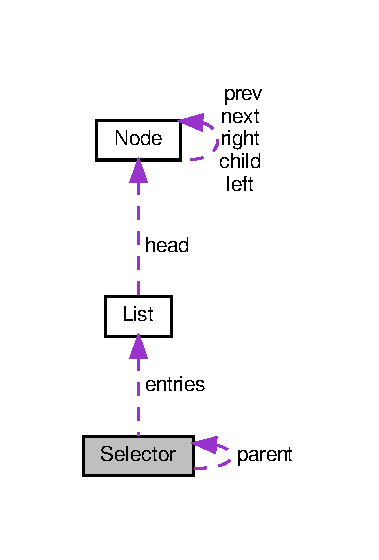
\includegraphics[width=182pt]{structSelector__coll__graph}
\end{center}
\end{figure}
\subsection*{Public Attributes}
\begin{DoxyCompactItemize}
\item 
char $\ast$ \hyperlink{structSelector_acbfa3c726e4642bb73866e111c977580}{title}
\item 
\hyperlink{structList}{List} $\ast$ \hyperlink{structSelector_ad83f9e77b597630270e0fa403fcd25ca}{entries}
\item 
\hyperlink{structSelector}{Selector} $\ast$ \hyperlink{structSelector_a628decf5829be812d3817aa5c98ac0e3}{parent}
\end{DoxyCompactItemize}


\subsection{Member Data Documentation}
\mbox{\Hypertarget{structSelector_ad83f9e77b597630270e0fa403fcd25ca}\label{structSelector_ad83f9e77b597630270e0fa403fcd25ca}} 
\index{Selector@{Selector}!entries@{entries}}
\index{entries@{entries}!Selector@{Selector}}
\subsubsection{\texorpdfstring{entries}{entries}}
{\footnotesize\ttfamily \hyperlink{structList}{List}$\ast$ Selector\+::entries}

\mbox{\Hypertarget{structSelector_a628decf5829be812d3817aa5c98ac0e3}\label{structSelector_a628decf5829be812d3817aa5c98ac0e3}} 
\index{Selector@{Selector}!parent@{parent}}
\index{parent@{parent}!Selector@{Selector}}
\subsubsection{\texorpdfstring{parent}{parent}}
{\footnotesize\ttfamily \hyperlink{structSelector}{Selector}$\ast$ Selector\+::parent}

\mbox{\Hypertarget{structSelector_acbfa3c726e4642bb73866e111c977580}\label{structSelector_acbfa3c726e4642bb73866e111c977580}} 
\index{Selector@{Selector}!title@{title}}
\index{title@{title}!Selector@{Selector}}
\subsubsection{\texorpdfstring{title}{title}}
{\footnotesize\ttfamily char$\ast$ Selector\+::title}



The documentation for this struct was generated from the following file\+:\begin{DoxyCompactItemize}
\item 
\hyperlink{selector_8h}{selector.\+h}\end{DoxyCompactItemize}

\hypertarget{structsetup__view}{}\section{setup\+\_\+view Struct Reference}
\label{structsetup__view}\index{setup\+\_\+view@{setup\+\_\+view}}


{\ttfamily \#include $<$graphics.\+h$>$}



Collaboration diagram for setup\+\_\+view\+:\nopagebreak
\begin{figure}[H]
\begin{center}
\leavevmode
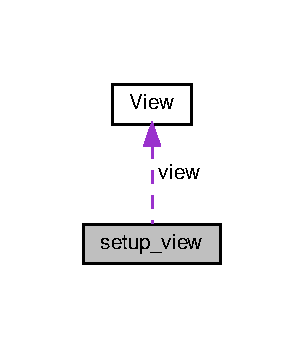
\includegraphics[width=146pt]{structsetup__view__coll__graph}
\end{center}
\end{figure}
\subsection*{Public Attributes}
\begin{DoxyCompactItemize}
\item 
\hyperlink{structView}{View} $\ast$ \hyperlink{structsetup__view_a480e2ffffe2e3294b565910c2fa55ee7}{view}
\end{DoxyCompactItemize}


\subsection{Member Data Documentation}
\mbox{\Hypertarget{structsetup__view_a480e2ffffe2e3294b565910c2fa55ee7}\label{structsetup__view_a480e2ffffe2e3294b565910c2fa55ee7}} 
\index{setup\+\_\+view@{setup\+\_\+view}!view@{view}}
\index{view@{view}!setup\+\_\+view@{setup\+\_\+view}}
\subsubsection{\texorpdfstring{view}{view}}
{\footnotesize\ttfamily \hyperlink{structView}{View}$\ast$ setup\+\_\+view\+::view}



The documentation for this struct was generated from the following file\+:\begin{DoxyCompactItemize}
\item 
\hyperlink{graphics_8h}{graphics.\+h}\end{DoxyCompactItemize}

\hypertarget{structView}{}\section{View Struct Reference}
\label{structView}\index{View@{View}}


{\ttfamily \#include $<$graphics.\+h$>$}

\subsection*{Public Attributes}
\begin{DoxyCompactItemize}
\item 
W\+I\+N\+D\+OW $\ast$ \hyperlink{structView_afae41b4d514883d788de11054c0a9596}{window}
\item 
unsigned char \hyperlink{structView_ad19f88e1766676afdf64e829d5120415}{inner\+\_\+width}
\item 
unsigned char \hyperlink{structView_a8085de6b2af6a9ada4df394f372d1c67}{inner\+\_\+height}
\item 
unsigned char \hyperlink{structView_adb64f0c8ad4030517a9a885b6232f60e}{outer\+\_\+width}
\item 
unsigned char \hyperlink{structView_af9ea34821bea7809441b35c2eafae471}{outer\+\_\+height}
\end{DoxyCompactItemize}


\subsection{Member Data Documentation}
\mbox{\Hypertarget{structView_a8085de6b2af6a9ada4df394f372d1c67}\label{structView_a8085de6b2af6a9ada4df394f372d1c67}} 
\index{View@{View}!inner\+\_\+height@{inner\+\_\+height}}
\index{inner\+\_\+height@{inner\+\_\+height}!View@{View}}
\subsubsection{\texorpdfstring{inner\+\_\+height}{inner\_height}}
{\footnotesize\ttfamily unsigned char View\+::inner\+\_\+height}

\mbox{\Hypertarget{structView_ad19f88e1766676afdf64e829d5120415}\label{structView_ad19f88e1766676afdf64e829d5120415}} 
\index{View@{View}!inner\+\_\+width@{inner\+\_\+width}}
\index{inner\+\_\+width@{inner\+\_\+width}!View@{View}}
\subsubsection{\texorpdfstring{inner\+\_\+width}{inner\_width}}
{\footnotesize\ttfamily unsigned char View\+::inner\+\_\+width}

\mbox{\Hypertarget{structView_af9ea34821bea7809441b35c2eafae471}\label{structView_af9ea34821bea7809441b35c2eafae471}} 
\index{View@{View}!outer\+\_\+height@{outer\+\_\+height}}
\index{outer\+\_\+height@{outer\+\_\+height}!View@{View}}
\subsubsection{\texorpdfstring{outer\+\_\+height}{outer\_height}}
{\footnotesize\ttfamily unsigned char View\+::outer\+\_\+height}

\mbox{\Hypertarget{structView_adb64f0c8ad4030517a9a885b6232f60e}\label{structView_adb64f0c8ad4030517a9a885b6232f60e}} 
\index{View@{View}!outer\+\_\+width@{outer\+\_\+width}}
\index{outer\+\_\+width@{outer\+\_\+width}!View@{View}}
\subsubsection{\texorpdfstring{outer\+\_\+width}{outer\_width}}
{\footnotesize\ttfamily unsigned char View\+::outer\+\_\+width}

\mbox{\Hypertarget{structView_afae41b4d514883d788de11054c0a9596}\label{structView_afae41b4d514883d788de11054c0a9596}} 
\index{View@{View}!window@{window}}
\index{window@{window}!View@{View}}
\subsubsection{\texorpdfstring{window}{window}}
{\footnotesize\ttfamily W\+I\+N\+D\+OW$\ast$ View\+::window}



The documentation for this struct was generated from the following file\+:\begin{DoxyCompactItemize}
\item 
\hyperlink{graphics_8h}{graphics.\+h}\end{DoxyCompactItemize}

\chapter{File Documentation}
\hypertarget{colors_8h}{}\section{colors.\+h File Reference}
\label{colors_8h}\index{colors.\+h@{colors.\+h}}
This graph shows which files directly or indirectly include this file\+:
\nopagebreak
\begin{figure}[H]
\begin{center}
\leavevmode
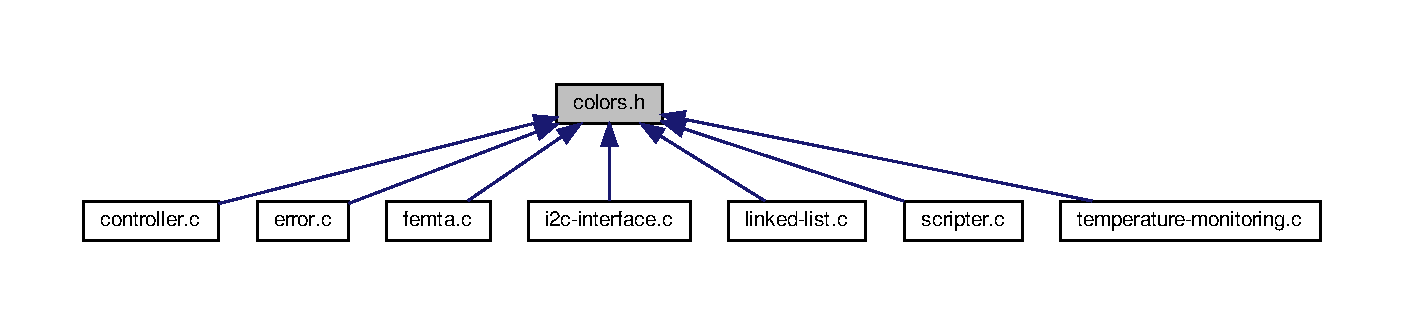
\includegraphics[width=350pt]{colors_8h__dep__incl}
\end{center}
\end{figure}
\subsection*{Macros}
\begin{DoxyCompactItemize}
\item 
\#define \hyperlink{colors_8h_a8d23feea868a983c8c2b661e1e16972f}{R\+ED}~\char`\"{}\textbackslash{}e\mbox{[}0;31m\char`\"{}
\item 
\#define \hyperlink{colors_8h_adce122f566c88a1eceeb79a635afa964}{G\+R\+EY}~\char`\"{}\textbackslash{}e\mbox{[}0;35m\char`\"{}
\item 
\#define \hyperlink{colors_8h_a79d10e672abb49ad63eeaa8aaef57c38}{B\+L\+UE}~\char`\"{}\textbackslash{}e\mbox{[}0;34m\char`\"{}
\item 
\#define \hyperlink{colors_8h_acfbc006ea433ad708fdee3e82996e721}{G\+R\+E\+EN}~\char`\"{}\textbackslash{}e\mbox{[}0;32m\char`\"{}
\item 
\#define \hyperlink{colors_8h_a0bb0b009e7a7390473ace4d98bd843c0}{P\+U\+R\+P\+LE}~\char`\"{}\textbackslash{}e\mbox{[}0;35m\char`\"{}
\item 
\#define \hyperlink{colors_8h_abf681265909adf3d3e8116c93c0ba179}{Y\+E\+L\+L\+OW}~\char`\"{}\textbackslash{}e\mbox{[}0;33m\char`\"{}
\item 
\#define \hyperlink{colors_8h_ab702106cf3b3e96750b6845ded4e0299}{R\+E\+S\+ET}~\char`\"{}\textbackslash{}e\mbox{[}0m\char`\"{}
\item 
\#define \hyperlink{colors_8h_ac25189db92959bff3c6c2adf4c34b50a}{D\+IM}~\char`\"{}\textbackslash{}e\mbox{[}2m\char`\"{}
\item 
\#define \hyperlink{colors_8h_a5d836bdb349c59eb6b385524054d3756}{U\+N\+D\+IM}~\char`\"{}\textbackslash{}e\mbox{[}22m\char`\"{}
\item 
\#define \hyperlink{colors_8h_a6972d3d624d2aeed390817b1d1b77ce8}{C\+O\+N\+S\+O\+L\+E\+\_\+\+R\+ED}~\char`\"{}\textbackslash{}e\mbox{[}31m\char`\"{}
\item 
\#define \hyperlink{colors_8h_a6031939572473bdc067eeb645d6b080e}{C\+O\+N\+S\+O\+L\+E\+\_\+\+G\+R\+E\+EN}~\char`\"{}\textbackslash{}e\mbox{[}32m\char`\"{}
\item 
\#define \hyperlink{colors_8h_a8e904b4ee6efda3d7017d4862766695e}{C\+O\+N\+S\+O\+L\+E\+\_\+\+Y\+E\+L\+L\+OW}~\char`\"{}\textbackslash{}e\mbox{[}33m\char`\"{}
\item 
\#define \hyperlink{colors_8h_ab1ea557c39ed061ef17bd2496cc57262}{C\+O\+N\+S\+O\+L\+E\+\_\+\+B\+L\+UE}~\char`\"{}\textbackslash{}e\mbox{[}34m\char`\"{}
\item 
\#define \hyperlink{colors_8h_acda5dd499ef491a51be79c1da5c077ff}{C\+O\+N\+S\+O\+L\+E\+\_\+\+M\+A\+G\+E\+N\+TA}~\char`\"{}\textbackslash{}e\mbox{[}35m\char`\"{}
\item 
\#define \hyperlink{colors_8h_aa2750ca2a5e52125aae9021551b7b346}{C\+O\+N\+S\+O\+L\+E\+\_\+\+C\+Y\+AN}~\char`\"{}\textbackslash{}e\mbox{[}36m\char`\"{}
\item 
\#define \hyperlink{colors_8h_aeffd764803863437d9b62b74d5ae5732}{C\+O\+N\+S\+O\+L\+E\+\_\+\+G\+R\+AY}~\char`\"{}\textbackslash{}e\mbox{[}37m\char`\"{}
\item 
\#define \hyperlink{colors_8h_a5bf9ac7b2fa0c4e790ed0750a2d548ac}{C\+O\+N\+S\+O\+L\+E\+\_\+\+R\+E\+S\+ET}~\char`\"{}\textbackslash{}e\mbox{[}39m\char`\"{}
\end{DoxyCompactItemize}


\subsection{Macro Definition Documentation}
\mbox{\Hypertarget{colors_8h_a79d10e672abb49ad63eeaa8aaef57c38}\label{colors_8h_a79d10e672abb49ad63eeaa8aaef57c38}} 
\index{colors.\+h@{colors.\+h}!B\+L\+UE@{B\+L\+UE}}
\index{B\+L\+UE@{B\+L\+UE}!colors.\+h@{colors.\+h}}
\subsubsection{\texorpdfstring{B\+L\+UE}{BLUE}}
{\footnotesize\ttfamily \#define B\+L\+UE~\char`\"{}\textbackslash{}e\mbox{[}0;34m\char`\"{}}

\mbox{\Hypertarget{colors_8h_ab1ea557c39ed061ef17bd2496cc57262}\label{colors_8h_ab1ea557c39ed061ef17bd2496cc57262}} 
\index{colors.\+h@{colors.\+h}!C\+O\+N\+S\+O\+L\+E\+\_\+\+B\+L\+UE@{C\+O\+N\+S\+O\+L\+E\+\_\+\+B\+L\+UE}}
\index{C\+O\+N\+S\+O\+L\+E\+\_\+\+B\+L\+UE@{C\+O\+N\+S\+O\+L\+E\+\_\+\+B\+L\+UE}!colors.\+h@{colors.\+h}}
\subsubsection{\texorpdfstring{C\+O\+N\+S\+O\+L\+E\+\_\+\+B\+L\+UE}{CONSOLE\_BLUE}}
{\footnotesize\ttfamily \#define C\+O\+N\+S\+O\+L\+E\+\_\+\+B\+L\+UE~\char`\"{}\textbackslash{}e\mbox{[}34m\char`\"{}}

\mbox{\Hypertarget{colors_8h_aa2750ca2a5e52125aae9021551b7b346}\label{colors_8h_aa2750ca2a5e52125aae9021551b7b346}} 
\index{colors.\+h@{colors.\+h}!C\+O\+N\+S\+O\+L\+E\+\_\+\+C\+Y\+AN@{C\+O\+N\+S\+O\+L\+E\+\_\+\+C\+Y\+AN}}
\index{C\+O\+N\+S\+O\+L\+E\+\_\+\+C\+Y\+AN@{C\+O\+N\+S\+O\+L\+E\+\_\+\+C\+Y\+AN}!colors.\+h@{colors.\+h}}
\subsubsection{\texorpdfstring{C\+O\+N\+S\+O\+L\+E\+\_\+\+C\+Y\+AN}{CONSOLE\_CYAN}}
{\footnotesize\ttfamily \#define C\+O\+N\+S\+O\+L\+E\+\_\+\+C\+Y\+AN~\char`\"{}\textbackslash{}e\mbox{[}36m\char`\"{}}

\mbox{\Hypertarget{colors_8h_aeffd764803863437d9b62b74d5ae5732}\label{colors_8h_aeffd764803863437d9b62b74d5ae5732}} 
\index{colors.\+h@{colors.\+h}!C\+O\+N\+S\+O\+L\+E\+\_\+\+G\+R\+AY@{C\+O\+N\+S\+O\+L\+E\+\_\+\+G\+R\+AY}}
\index{C\+O\+N\+S\+O\+L\+E\+\_\+\+G\+R\+AY@{C\+O\+N\+S\+O\+L\+E\+\_\+\+G\+R\+AY}!colors.\+h@{colors.\+h}}
\subsubsection{\texorpdfstring{C\+O\+N\+S\+O\+L\+E\+\_\+\+G\+R\+AY}{CONSOLE\_GRAY}}
{\footnotesize\ttfamily \#define C\+O\+N\+S\+O\+L\+E\+\_\+\+G\+R\+AY~\char`\"{}\textbackslash{}e\mbox{[}37m\char`\"{}}

\mbox{\Hypertarget{colors_8h_a6031939572473bdc067eeb645d6b080e}\label{colors_8h_a6031939572473bdc067eeb645d6b080e}} 
\index{colors.\+h@{colors.\+h}!C\+O\+N\+S\+O\+L\+E\+\_\+\+G\+R\+E\+EN@{C\+O\+N\+S\+O\+L\+E\+\_\+\+G\+R\+E\+EN}}
\index{C\+O\+N\+S\+O\+L\+E\+\_\+\+G\+R\+E\+EN@{C\+O\+N\+S\+O\+L\+E\+\_\+\+G\+R\+E\+EN}!colors.\+h@{colors.\+h}}
\subsubsection{\texorpdfstring{C\+O\+N\+S\+O\+L\+E\+\_\+\+G\+R\+E\+EN}{CONSOLE\_GREEN}}
{\footnotesize\ttfamily \#define C\+O\+N\+S\+O\+L\+E\+\_\+\+G\+R\+E\+EN~\char`\"{}\textbackslash{}e\mbox{[}32m\char`\"{}}

\mbox{\Hypertarget{colors_8h_acda5dd499ef491a51be79c1da5c077ff}\label{colors_8h_acda5dd499ef491a51be79c1da5c077ff}} 
\index{colors.\+h@{colors.\+h}!C\+O\+N\+S\+O\+L\+E\+\_\+\+M\+A\+G\+E\+N\+TA@{C\+O\+N\+S\+O\+L\+E\+\_\+\+M\+A\+G\+E\+N\+TA}}
\index{C\+O\+N\+S\+O\+L\+E\+\_\+\+M\+A\+G\+E\+N\+TA@{C\+O\+N\+S\+O\+L\+E\+\_\+\+M\+A\+G\+E\+N\+TA}!colors.\+h@{colors.\+h}}
\subsubsection{\texorpdfstring{C\+O\+N\+S\+O\+L\+E\+\_\+\+M\+A\+G\+E\+N\+TA}{CONSOLE\_MAGENTA}}
{\footnotesize\ttfamily \#define C\+O\+N\+S\+O\+L\+E\+\_\+\+M\+A\+G\+E\+N\+TA~\char`\"{}\textbackslash{}e\mbox{[}35m\char`\"{}}

\mbox{\Hypertarget{colors_8h_a6972d3d624d2aeed390817b1d1b77ce8}\label{colors_8h_a6972d3d624d2aeed390817b1d1b77ce8}} 
\index{colors.\+h@{colors.\+h}!C\+O\+N\+S\+O\+L\+E\+\_\+\+R\+ED@{C\+O\+N\+S\+O\+L\+E\+\_\+\+R\+ED}}
\index{C\+O\+N\+S\+O\+L\+E\+\_\+\+R\+ED@{C\+O\+N\+S\+O\+L\+E\+\_\+\+R\+ED}!colors.\+h@{colors.\+h}}
\subsubsection{\texorpdfstring{C\+O\+N\+S\+O\+L\+E\+\_\+\+R\+ED}{CONSOLE\_RED}}
{\footnotesize\ttfamily \#define C\+O\+N\+S\+O\+L\+E\+\_\+\+R\+ED~\char`\"{}\textbackslash{}e\mbox{[}31m\char`\"{}}

\mbox{\Hypertarget{colors_8h_a5bf9ac7b2fa0c4e790ed0750a2d548ac}\label{colors_8h_a5bf9ac7b2fa0c4e790ed0750a2d548ac}} 
\index{colors.\+h@{colors.\+h}!C\+O\+N\+S\+O\+L\+E\+\_\+\+R\+E\+S\+ET@{C\+O\+N\+S\+O\+L\+E\+\_\+\+R\+E\+S\+ET}}
\index{C\+O\+N\+S\+O\+L\+E\+\_\+\+R\+E\+S\+ET@{C\+O\+N\+S\+O\+L\+E\+\_\+\+R\+E\+S\+ET}!colors.\+h@{colors.\+h}}
\subsubsection{\texorpdfstring{C\+O\+N\+S\+O\+L\+E\+\_\+\+R\+E\+S\+ET}{CONSOLE\_RESET}}
{\footnotesize\ttfamily \#define C\+O\+N\+S\+O\+L\+E\+\_\+\+R\+E\+S\+ET~\char`\"{}\textbackslash{}e\mbox{[}39m\char`\"{}}

\mbox{\Hypertarget{colors_8h_a8e904b4ee6efda3d7017d4862766695e}\label{colors_8h_a8e904b4ee6efda3d7017d4862766695e}} 
\index{colors.\+h@{colors.\+h}!C\+O\+N\+S\+O\+L\+E\+\_\+\+Y\+E\+L\+L\+OW@{C\+O\+N\+S\+O\+L\+E\+\_\+\+Y\+E\+L\+L\+OW}}
\index{C\+O\+N\+S\+O\+L\+E\+\_\+\+Y\+E\+L\+L\+OW@{C\+O\+N\+S\+O\+L\+E\+\_\+\+Y\+E\+L\+L\+OW}!colors.\+h@{colors.\+h}}
\subsubsection{\texorpdfstring{C\+O\+N\+S\+O\+L\+E\+\_\+\+Y\+E\+L\+L\+OW}{CONSOLE\_YELLOW}}
{\footnotesize\ttfamily \#define C\+O\+N\+S\+O\+L\+E\+\_\+\+Y\+E\+L\+L\+OW~\char`\"{}\textbackslash{}e\mbox{[}33m\char`\"{}}

\mbox{\Hypertarget{colors_8h_ac25189db92959bff3c6c2adf4c34b50a}\label{colors_8h_ac25189db92959bff3c6c2adf4c34b50a}} 
\index{colors.\+h@{colors.\+h}!D\+IM@{D\+IM}}
\index{D\+IM@{D\+IM}!colors.\+h@{colors.\+h}}
\subsubsection{\texorpdfstring{D\+IM}{DIM}}
{\footnotesize\ttfamily \#define D\+IM~\char`\"{}\textbackslash{}e\mbox{[}2m\char`\"{}}

\mbox{\Hypertarget{colors_8h_acfbc006ea433ad708fdee3e82996e721}\label{colors_8h_acfbc006ea433ad708fdee3e82996e721}} 
\index{colors.\+h@{colors.\+h}!G\+R\+E\+EN@{G\+R\+E\+EN}}
\index{G\+R\+E\+EN@{G\+R\+E\+EN}!colors.\+h@{colors.\+h}}
\subsubsection{\texorpdfstring{G\+R\+E\+EN}{GREEN}}
{\footnotesize\ttfamily \#define G\+R\+E\+EN~\char`\"{}\textbackslash{}e\mbox{[}0;32m\char`\"{}}

\mbox{\Hypertarget{colors_8h_adce122f566c88a1eceeb79a635afa964}\label{colors_8h_adce122f566c88a1eceeb79a635afa964}} 
\index{colors.\+h@{colors.\+h}!G\+R\+EY@{G\+R\+EY}}
\index{G\+R\+EY@{G\+R\+EY}!colors.\+h@{colors.\+h}}
\subsubsection{\texorpdfstring{G\+R\+EY}{GREY}}
{\footnotesize\ttfamily \#define G\+R\+EY~\char`\"{}\textbackslash{}e\mbox{[}0;35m\char`\"{}}

\mbox{\Hypertarget{colors_8h_a0bb0b009e7a7390473ace4d98bd843c0}\label{colors_8h_a0bb0b009e7a7390473ace4d98bd843c0}} 
\index{colors.\+h@{colors.\+h}!P\+U\+R\+P\+LE@{P\+U\+R\+P\+LE}}
\index{P\+U\+R\+P\+LE@{P\+U\+R\+P\+LE}!colors.\+h@{colors.\+h}}
\subsubsection{\texorpdfstring{P\+U\+R\+P\+LE}{PURPLE}}
{\footnotesize\ttfamily \#define P\+U\+R\+P\+LE~\char`\"{}\textbackslash{}e\mbox{[}0;35m\char`\"{}}

\mbox{\Hypertarget{colors_8h_a8d23feea868a983c8c2b661e1e16972f}\label{colors_8h_a8d23feea868a983c8c2b661e1e16972f}} 
\index{colors.\+h@{colors.\+h}!R\+ED@{R\+ED}}
\index{R\+ED@{R\+ED}!colors.\+h@{colors.\+h}}
\subsubsection{\texorpdfstring{R\+ED}{RED}}
{\footnotesize\ttfamily \#define R\+ED~\char`\"{}\textbackslash{}e\mbox{[}0;31m\char`\"{}}

\mbox{\Hypertarget{colors_8h_ab702106cf3b3e96750b6845ded4e0299}\label{colors_8h_ab702106cf3b3e96750b6845ded4e0299}} 
\index{colors.\+h@{colors.\+h}!R\+E\+S\+ET@{R\+E\+S\+ET}}
\index{R\+E\+S\+ET@{R\+E\+S\+ET}!colors.\+h@{colors.\+h}}
\subsubsection{\texorpdfstring{R\+E\+S\+ET}{RESET}}
{\footnotesize\ttfamily \#define R\+E\+S\+ET~\char`\"{}\textbackslash{}e\mbox{[}0m\char`\"{}}

\mbox{\Hypertarget{colors_8h_a5d836bdb349c59eb6b385524054d3756}\label{colors_8h_a5d836bdb349c59eb6b385524054d3756}} 
\index{colors.\+h@{colors.\+h}!U\+N\+D\+IM@{U\+N\+D\+IM}}
\index{U\+N\+D\+IM@{U\+N\+D\+IM}!colors.\+h@{colors.\+h}}
\subsubsection{\texorpdfstring{U\+N\+D\+IM}{UNDIM}}
{\footnotesize\ttfamily \#define U\+N\+D\+IM~\char`\"{}\textbackslash{}e\mbox{[}22m\char`\"{}}

\mbox{\Hypertarget{colors_8h_abf681265909adf3d3e8116c93c0ba179}\label{colors_8h_abf681265909adf3d3e8116c93c0ba179}} 
\index{colors.\+h@{colors.\+h}!Y\+E\+L\+L\+OW@{Y\+E\+L\+L\+OW}}
\index{Y\+E\+L\+L\+OW@{Y\+E\+L\+L\+OW}!colors.\+h@{colors.\+h}}
\subsubsection{\texorpdfstring{Y\+E\+L\+L\+OW}{YELLOW}}
{\footnotesize\ttfamily \#define Y\+E\+L\+L\+OW~\char`\"{}\textbackslash{}e\mbox{[}0;33m\char`\"{}}


\hypertarget{controller_8c}{}\section{controller.\+c File Reference}
\label{controller_8c}\index{controller.\+c@{controller.\+c}}
{\ttfamily \#include $<$stdlib.\+h$>$}\newline
{\ttfamily \#include $<$stdio.\+h$>$}\newline
{\ttfamily \#include $<$unistd.\+h$>$}\newline
{\ttfamily \#include $<$math.\+h$>$}\newline
{\ttfamily \#include \char`\"{}femta.\+h\char`\"{}}\newline
{\ttfamily \#include \char`\"{}controller.\+h\char`\"{}}\newline
{\ttfamily \#include \char`\"{}quaternion.\+h\char`\"{}}\newline
{\ttfamily \#include \char`\"{}graphics.\+h\char`\"{}}\newline
{\ttfamily \#include \char`\"{}selector.\+h\char`\"{}}\newline
{\ttfamily \#include \char`\"{}colors.\+h\char`\"{}}\newline
Include dependency graph for controller.\+c\+:
\nopagebreak
\begin{figure}[H]
\begin{center}
\leavevmode
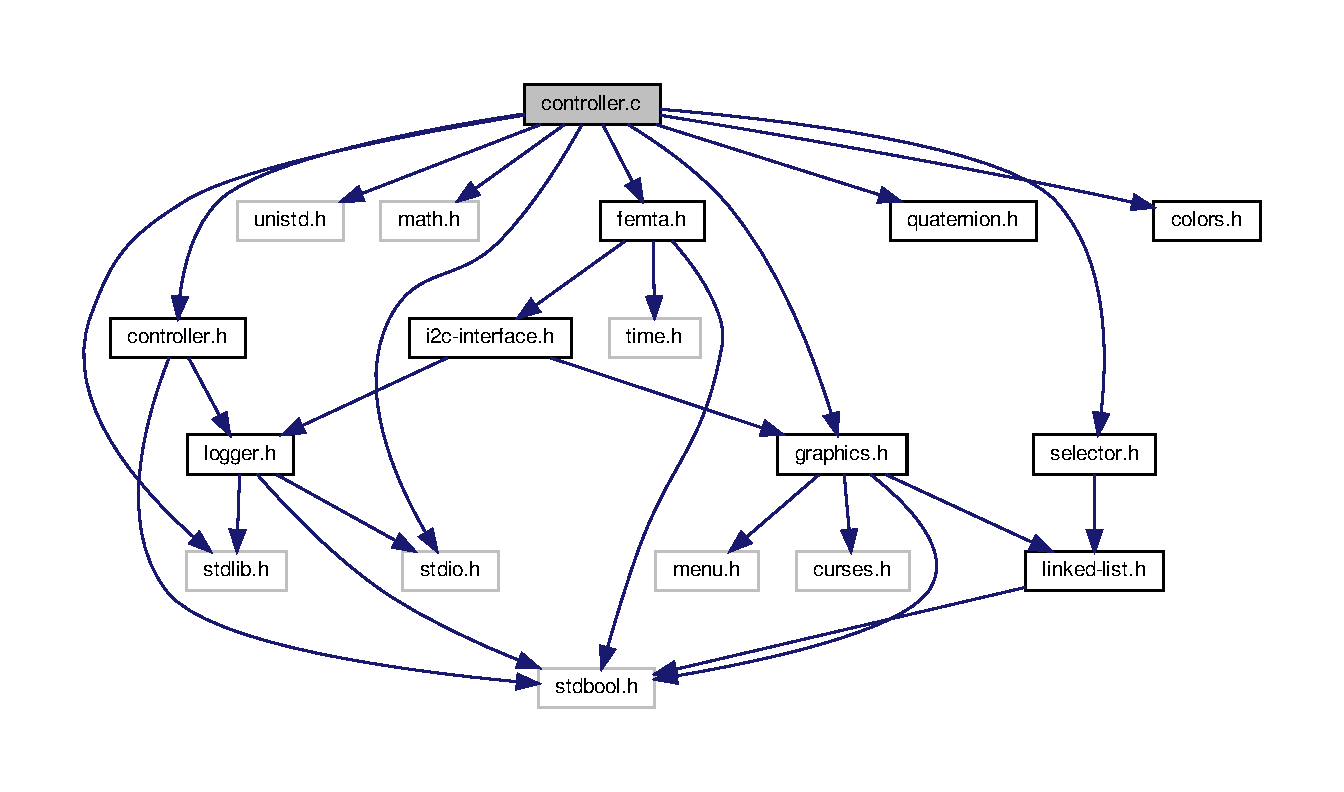
\includegraphics[width=350pt]{controller_8c__incl}
\end{center}
\end{figure}
\subsection*{Functions}
\begin{DoxyCompactItemize}
\item 
void \hyperlink{controller_8c_aeefc9e02ca647cde356037b5033166fd}{ramp\+\_\+up} (void $\ast$nil)
\item 
void \hyperlink{controller_8c_a3d51d5067e0c5307f18a9145f3592fd0}{pyramid} (int stepsize, int timebtwn)
\item 
void \hyperlink{controller_8c_a3478671fc5f77ca4e08ee1b5db9959bf}{set\+\_\+bank\+\_\+speed} (bool CW, bool C\+CW, int pwm\+\_\+num)
\item 
float \hyperlink{controller_8c_af32126493fe3a94e43889aaf5f28d564}{rise\+\_\+time} (float phi\+\_\+des)
\item 
float \hyperlink{controller_8c_a26016d59d4d9df342535c2af5439f3c6}{tracking\+\_\+signal\+\_\+value} (int phi\+\_\+des, float t, float tr)
\item 
float \hyperlink{controller_8c_a6500da947313d9327a5f4486abaf9b3c}{get\+\_\+mpu\+\_\+val} ()
\item 
void \hyperlink{controller_8c_a8cb8a5d01aea8b1d058f09bd99b92b69}{P\+I\+D\+\_\+controller} (bool CW, bool C\+CW, float init\+\_\+or, float dor)
\end{DoxyCompactItemize}
\subsection*{Variables}
\begin{DoxyCompactItemize}
\item 
int \hyperlink{controller_8c_af3fe4c736af2b19d876092efa53b6387}{default\+\_\+step\+\_\+size} = 0
\item 
int \hyperlink{controller_8c_a8ce073b16d7d349ed4170223fa2a4520}{default\+\_\+time\+\_\+between} = 0
\end{DoxyCompactItemize}


\subsection{Function Documentation}
\mbox{\Hypertarget{controller_8c_a6500da947313d9327a5f4486abaf9b3c}\label{controller_8c_a6500da947313d9327a5f4486abaf9b3c}} 
\index{controller.\+c@{controller.\+c}!get\+\_\+mpu\+\_\+val@{get\+\_\+mpu\+\_\+val}}
\index{get\+\_\+mpu\+\_\+val@{get\+\_\+mpu\+\_\+val}!controller.\+c@{controller.\+c}}
\subsubsection{\texorpdfstring{get\+\_\+mpu\+\_\+val()}{get\_mpu\_val()}}
{\footnotesize\ttfamily float get\+\_\+mpu\+\_\+val (\begin{DoxyParamCaption}{ }\end{DoxyParamCaption})}

\mbox{\Hypertarget{controller_8c_a8cb8a5d01aea8b1d058f09bd99b92b69}\label{controller_8c_a8cb8a5d01aea8b1d058f09bd99b92b69}} 
\index{controller.\+c@{controller.\+c}!P\+I\+D\+\_\+controller@{P\+I\+D\+\_\+controller}}
\index{P\+I\+D\+\_\+controller@{P\+I\+D\+\_\+controller}!controller.\+c@{controller.\+c}}
\subsubsection{\texorpdfstring{P\+I\+D\+\_\+controller()}{PID\_controller()}}
{\footnotesize\ttfamily void P\+I\+D\+\_\+controller (\begin{DoxyParamCaption}\item[{bool}]{CW,  }\item[{bool}]{C\+CW,  }\item[{float}]{init\+\_\+or,  }\item[{float}]{dor }\end{DoxyParamCaption})}

\mbox{\Hypertarget{controller_8c_a3d51d5067e0c5307f18a9145f3592fd0}\label{controller_8c_a3d51d5067e0c5307f18a9145f3592fd0}} 
\index{controller.\+c@{controller.\+c}!pyramid@{pyramid}}
\index{pyramid@{pyramid}!controller.\+c@{controller.\+c}}
\subsubsection{\texorpdfstring{pyramid()}{pyramid()}}
{\footnotesize\ttfamily void pyramid (\begin{DoxyParamCaption}\item[{int}]{stepsize,  }\item[{int}]{timebtwn }\end{DoxyParamCaption})}

Here is the call graph for this function\+:
\nopagebreak
\begin{figure}[H]
\begin{center}
\leavevmode
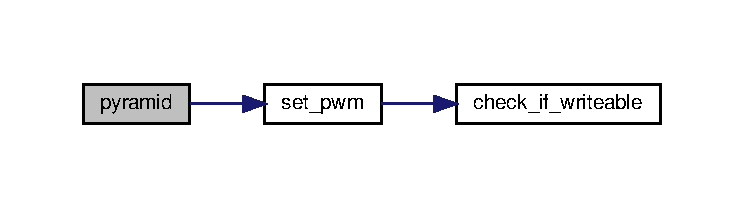
\includegraphics[width=350pt]{controller_8c_a3d51d5067e0c5307f18a9145f3592fd0_cgraph}
\end{center}
\end{figure}
\mbox{\Hypertarget{controller_8c_aeefc9e02ca647cde356037b5033166fd}\label{controller_8c_aeefc9e02ca647cde356037b5033166fd}} 
\index{controller.\+c@{controller.\+c}!ramp\+\_\+up@{ramp\+\_\+up}}
\index{ramp\+\_\+up@{ramp\+\_\+up}!controller.\+c@{controller.\+c}}
\subsubsection{\texorpdfstring{ramp\+\_\+up()}{ramp\_up()}}
{\footnotesize\ttfamily void ramp\+\_\+up (\begin{DoxyParamCaption}\item[{void $\ast$}]{nil }\end{DoxyParamCaption})}

Here is the call graph for this function\+:
\nopagebreak
\begin{figure}[H]
\begin{center}
\leavevmode
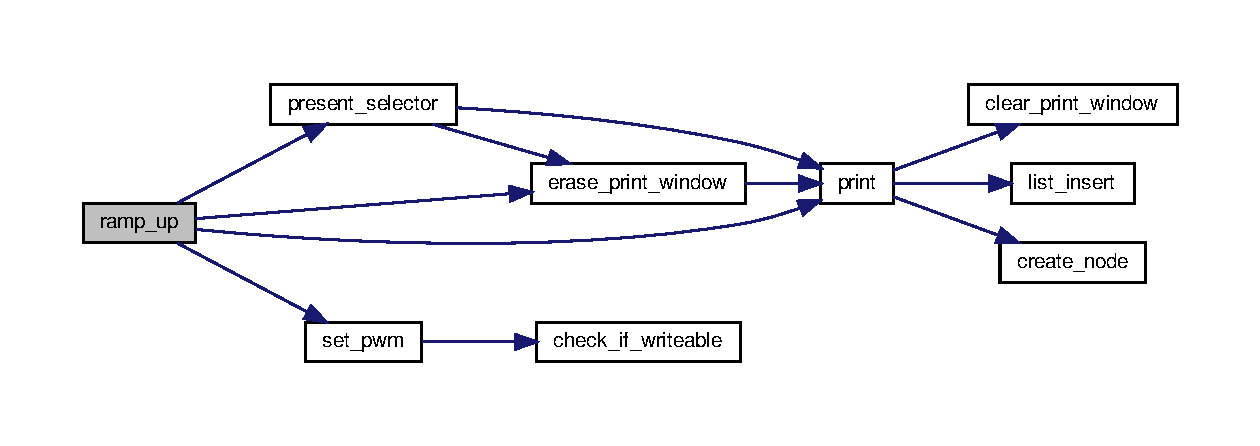
\includegraphics[width=350pt]{controller_8c_aeefc9e02ca647cde356037b5033166fd_cgraph}
\end{center}
\end{figure}
Here is the caller graph for this function\+:
\nopagebreak
\begin{figure}[H]
\begin{center}
\leavevmode
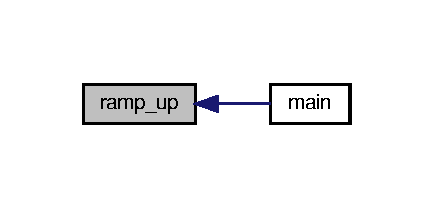
\includegraphics[width=208pt]{controller_8c_aeefc9e02ca647cde356037b5033166fd_icgraph}
\end{center}
\end{figure}
\mbox{\Hypertarget{controller_8c_af32126493fe3a94e43889aaf5f28d564}\label{controller_8c_af32126493fe3a94e43889aaf5f28d564}} 
\index{controller.\+c@{controller.\+c}!rise\+\_\+time@{rise\+\_\+time}}
\index{rise\+\_\+time@{rise\+\_\+time}!controller.\+c@{controller.\+c}}
\subsubsection{\texorpdfstring{rise\+\_\+time()}{rise\_time()}}
{\footnotesize\ttfamily float rise\+\_\+time (\begin{DoxyParamCaption}\item[{float}]{phi\+\_\+des }\end{DoxyParamCaption})}

\mbox{\Hypertarget{controller_8c_a3478671fc5f77ca4e08ee1b5db9959bf}\label{controller_8c_a3478671fc5f77ca4e08ee1b5db9959bf}} 
\index{controller.\+c@{controller.\+c}!set\+\_\+bank\+\_\+speed@{set\+\_\+bank\+\_\+speed}}
\index{set\+\_\+bank\+\_\+speed@{set\+\_\+bank\+\_\+speed}!controller.\+c@{controller.\+c}}
\subsubsection{\texorpdfstring{set\+\_\+bank\+\_\+speed()}{set\_bank\_speed()}}
{\footnotesize\ttfamily void set\+\_\+bank\+\_\+speed (\begin{DoxyParamCaption}\item[{bool}]{CW,  }\item[{bool}]{C\+CW,  }\item[{int}]{pwm\+\_\+num }\end{DoxyParamCaption})}

Here is the call graph for this function\+:
\nopagebreak
\begin{figure}[H]
\begin{center}
\leavevmode
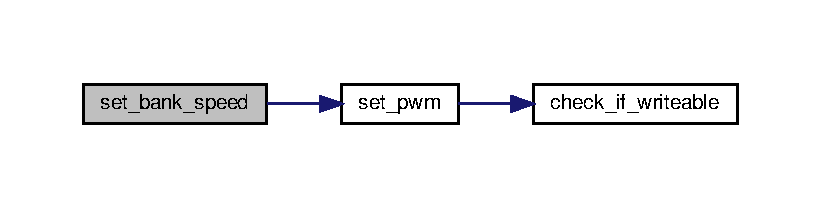
\includegraphics[width=350pt]{controller_8c_a3478671fc5f77ca4e08ee1b5db9959bf_cgraph}
\end{center}
\end{figure}
\mbox{\Hypertarget{controller_8c_a26016d59d4d9df342535c2af5439f3c6}\label{controller_8c_a26016d59d4d9df342535c2af5439f3c6}} 
\index{controller.\+c@{controller.\+c}!tracking\+\_\+signal\+\_\+value@{tracking\+\_\+signal\+\_\+value}}
\index{tracking\+\_\+signal\+\_\+value@{tracking\+\_\+signal\+\_\+value}!controller.\+c@{controller.\+c}}
\subsubsection{\texorpdfstring{tracking\+\_\+signal\+\_\+value()}{tracking\_signal\_value()}}
{\footnotesize\ttfamily float tracking\+\_\+signal\+\_\+value (\begin{DoxyParamCaption}\item[{int}]{phi\+\_\+des,  }\item[{float}]{t,  }\item[{float}]{tr }\end{DoxyParamCaption})}



\subsection{Variable Documentation}
\mbox{\Hypertarget{controller_8c_af3fe4c736af2b19d876092efa53b6387}\label{controller_8c_af3fe4c736af2b19d876092efa53b6387}} 
\index{controller.\+c@{controller.\+c}!default\+\_\+step\+\_\+size@{default\+\_\+step\+\_\+size}}
\index{default\+\_\+step\+\_\+size@{default\+\_\+step\+\_\+size}!controller.\+c@{controller.\+c}}
\subsubsection{\texorpdfstring{default\+\_\+step\+\_\+size}{default\_step\_size}}
{\footnotesize\ttfamily int default\+\_\+step\+\_\+size = 0}

\mbox{\Hypertarget{controller_8c_a8ce073b16d7d349ed4170223fa2a4520}\label{controller_8c_a8ce073b16d7d349ed4170223fa2a4520}} 
\index{controller.\+c@{controller.\+c}!default\+\_\+time\+\_\+between@{default\+\_\+time\+\_\+between}}
\index{default\+\_\+time\+\_\+between@{default\+\_\+time\+\_\+between}!controller.\+c@{controller.\+c}}
\subsubsection{\texorpdfstring{default\+\_\+time\+\_\+between}{default\_time\_between}}
{\footnotesize\ttfamily int default\+\_\+time\+\_\+between = 0}


\hypertarget{controller_8h}{}\section{controller.\+h File Reference}
\label{controller_8h}\index{controller.\+h@{controller.\+h}}
{\ttfamily \#include $<$stdbool.\+h$>$}\newline
{\ttfamily \#include \char`\"{}logger.\+h\char`\"{}}\newline
Include dependency graph for controller.\+h\+:
\nopagebreak
\begin{figure}[H]
\begin{center}
\leavevmode
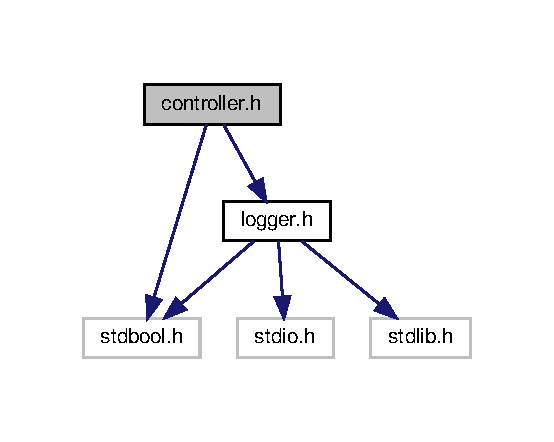
\includegraphics[width=266pt]{controller_8h__incl}
\end{center}
\end{figure}
This graph shows which files directly or indirectly include this file\+:
\nopagebreak
\begin{figure}[H]
\begin{center}
\leavevmode
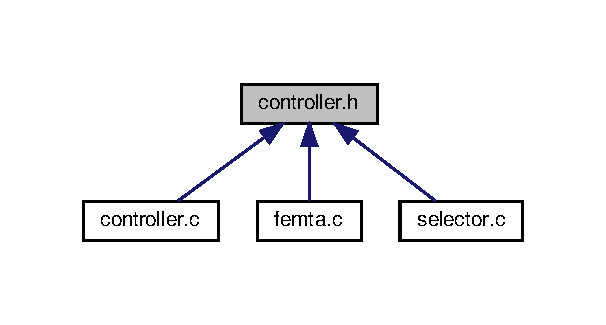
\includegraphics[width=291pt]{controller_8h__dep__incl}
\end{center}
\end{figure}
\subsection*{Macros}
\begin{DoxyCompactItemize}
\item 
\#define \hyperlink{controller_8h_ad99541aad779a151a2ce44d12214e6a4}{M\+I\+N\+\_\+\+S\+AT}~0
\item 
\#define \hyperlink{controller_8h_a1df990f1a1fc97b95e8d53f719968026}{M\+A\+X\+\_\+\+P\+WM}~0
\item 
\#define \hyperlink{controller_8h_af95a8419331447992b52df951bfd51aa}{P\+I\+D\+\_\+\+E\+R\+R\+\_\+\+T\+OL}~0.\+05
\item 
\#define \hyperlink{controller_8h_a598a3330b3c21701223ee0ca14316eca}{PI}~3.\+14159265
\end{DoxyCompactItemize}
\subsection*{Functions}
\begin{DoxyCompactItemize}
\item 
void \hyperlink{controller_8h_aeefc9e02ca647cde356037b5033166fd}{ramp\+\_\+up} (void $\ast$nil)
\item 
void \hyperlink{controller_8h_a3d51d5067e0c5307f18a9145f3592fd0}{pyramid} (int stepsize, int timebtwn)
\item 
void \hyperlink{controller_8h_a79cb74a64d9173f1412a2b261d7ac82f}{set\+\_\+bank\+\_\+speed} (bool CW, bool C\+CW, int pwn\+\_\+num)
\item 
float \hyperlink{controller_8h_af32126493fe3a94e43889aaf5f28d564}{rise\+\_\+time} (float phi\+\_\+des)
\item 
float \hyperlink{controller_8h_a26016d59d4d9df342535c2af5439f3c6}{tracking\+\_\+signal\+\_\+value} (int phi\+\_\+des, float t, float tr)
\item 
void \hyperlink{controller_8h_a8cb8a5d01aea8b1d058f09bd99b92b69}{P\+I\+D\+\_\+controller} (bool CW, bool C\+CW, float init\+\_\+or, float dor)
\end{DoxyCompactItemize}
\subsection*{Variables}
\begin{DoxyCompactItemize}
\item 
\hyperlink{structLogger}{Logger} $\ast$ \hyperlink{controller_8h_ae3b00f80c9797211832566f1b2cff771}{pid\+\_\+logger}
\end{DoxyCompactItemize}


\subsection{Macro Definition Documentation}
\mbox{\Hypertarget{controller_8h_a1df990f1a1fc97b95e8d53f719968026}\label{controller_8h_a1df990f1a1fc97b95e8d53f719968026}} 
\index{controller.\+h@{controller.\+h}!M\+A\+X\+\_\+\+P\+WM@{M\+A\+X\+\_\+\+P\+WM}}
\index{M\+A\+X\+\_\+\+P\+WM@{M\+A\+X\+\_\+\+P\+WM}!controller.\+h@{controller.\+h}}
\subsubsection{\texorpdfstring{M\+A\+X\+\_\+\+P\+WM}{MAX\_PWM}}
{\footnotesize\ttfamily \#define M\+A\+X\+\_\+\+P\+WM~0}

\mbox{\Hypertarget{controller_8h_ad99541aad779a151a2ce44d12214e6a4}\label{controller_8h_ad99541aad779a151a2ce44d12214e6a4}} 
\index{controller.\+h@{controller.\+h}!M\+I\+N\+\_\+\+S\+AT@{M\+I\+N\+\_\+\+S\+AT}}
\index{M\+I\+N\+\_\+\+S\+AT@{M\+I\+N\+\_\+\+S\+AT}!controller.\+h@{controller.\+h}}
\subsubsection{\texorpdfstring{M\+I\+N\+\_\+\+S\+AT}{MIN\_SAT}}
{\footnotesize\ttfamily \#define M\+I\+N\+\_\+\+S\+AT~0}

\mbox{\Hypertarget{controller_8h_a598a3330b3c21701223ee0ca14316eca}\label{controller_8h_a598a3330b3c21701223ee0ca14316eca}} 
\index{controller.\+h@{controller.\+h}!PI@{PI}}
\index{PI@{PI}!controller.\+h@{controller.\+h}}
\subsubsection{\texorpdfstring{PI}{PI}}
{\footnotesize\ttfamily \#define PI~3.\+14159265}

\mbox{\Hypertarget{controller_8h_af95a8419331447992b52df951bfd51aa}\label{controller_8h_af95a8419331447992b52df951bfd51aa}} 
\index{controller.\+h@{controller.\+h}!P\+I\+D\+\_\+\+E\+R\+R\+\_\+\+T\+OL@{P\+I\+D\+\_\+\+E\+R\+R\+\_\+\+T\+OL}}
\index{P\+I\+D\+\_\+\+E\+R\+R\+\_\+\+T\+OL@{P\+I\+D\+\_\+\+E\+R\+R\+\_\+\+T\+OL}!controller.\+h@{controller.\+h}}
\subsubsection{\texorpdfstring{P\+I\+D\+\_\+\+E\+R\+R\+\_\+\+T\+OL}{PID\_ERR\_TOL}}
{\footnotesize\ttfamily \#define P\+I\+D\+\_\+\+E\+R\+R\+\_\+\+T\+OL~0.\+05}



\subsection{Function Documentation}
\mbox{\Hypertarget{controller_8h_a8cb8a5d01aea8b1d058f09bd99b92b69}\label{controller_8h_a8cb8a5d01aea8b1d058f09bd99b92b69}} 
\index{controller.\+h@{controller.\+h}!P\+I\+D\+\_\+controller@{P\+I\+D\+\_\+controller}}
\index{P\+I\+D\+\_\+controller@{P\+I\+D\+\_\+controller}!controller.\+h@{controller.\+h}}
\subsubsection{\texorpdfstring{P\+I\+D\+\_\+controller()}{PID\_controller()}}
{\footnotesize\ttfamily void P\+I\+D\+\_\+controller (\begin{DoxyParamCaption}\item[{bool}]{CW,  }\item[{bool}]{C\+CW,  }\item[{float}]{init\+\_\+or,  }\item[{float}]{dor }\end{DoxyParamCaption})}

\mbox{\Hypertarget{controller_8h_a3d51d5067e0c5307f18a9145f3592fd0}\label{controller_8h_a3d51d5067e0c5307f18a9145f3592fd0}} 
\index{controller.\+h@{controller.\+h}!pyramid@{pyramid}}
\index{pyramid@{pyramid}!controller.\+h@{controller.\+h}}
\subsubsection{\texorpdfstring{pyramid()}{pyramid()}}
{\footnotesize\ttfamily void pyramid (\begin{DoxyParamCaption}\item[{int}]{stepsize,  }\item[{int}]{timebtwn }\end{DoxyParamCaption})}

Here is the call graph for this function\+:
\nopagebreak
\begin{figure}[H]
\begin{center}
\leavevmode
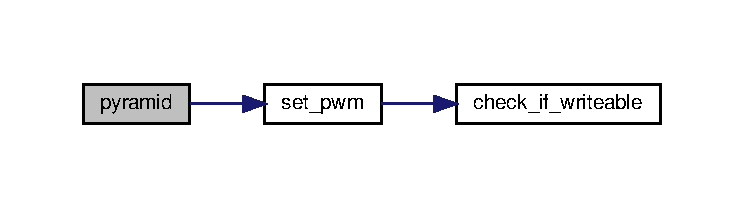
\includegraphics[width=350pt]{controller_8h_a3d51d5067e0c5307f18a9145f3592fd0_cgraph}
\end{center}
\end{figure}
\mbox{\Hypertarget{controller_8h_aeefc9e02ca647cde356037b5033166fd}\label{controller_8h_aeefc9e02ca647cde356037b5033166fd}} 
\index{controller.\+h@{controller.\+h}!ramp\+\_\+up@{ramp\+\_\+up}}
\index{ramp\+\_\+up@{ramp\+\_\+up}!controller.\+h@{controller.\+h}}
\subsubsection{\texorpdfstring{ramp\+\_\+up()}{ramp\_up()}}
{\footnotesize\ttfamily void ramp\+\_\+up (\begin{DoxyParamCaption}\item[{void $\ast$}]{nil }\end{DoxyParamCaption})}

Here is the call graph for this function\+:
\nopagebreak
\begin{figure}[H]
\begin{center}
\leavevmode
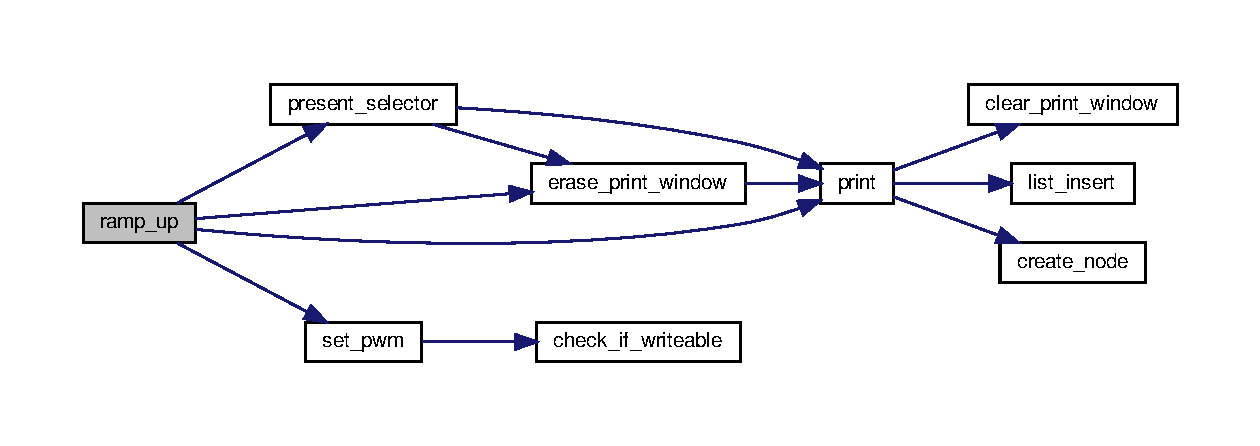
\includegraphics[width=350pt]{controller_8h_aeefc9e02ca647cde356037b5033166fd_cgraph}
\end{center}
\end{figure}
Here is the caller graph for this function\+:
\nopagebreak
\begin{figure}[H]
\begin{center}
\leavevmode
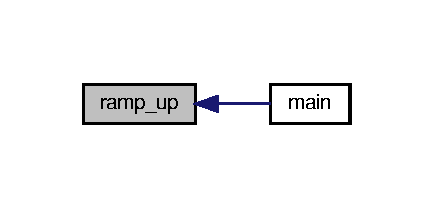
\includegraphics[width=208pt]{controller_8h_aeefc9e02ca647cde356037b5033166fd_icgraph}
\end{center}
\end{figure}
\mbox{\Hypertarget{controller_8h_af32126493fe3a94e43889aaf5f28d564}\label{controller_8h_af32126493fe3a94e43889aaf5f28d564}} 
\index{controller.\+h@{controller.\+h}!rise\+\_\+time@{rise\+\_\+time}}
\index{rise\+\_\+time@{rise\+\_\+time}!controller.\+h@{controller.\+h}}
\subsubsection{\texorpdfstring{rise\+\_\+time()}{rise\_time()}}
{\footnotesize\ttfamily float rise\+\_\+time (\begin{DoxyParamCaption}\item[{float}]{phi\+\_\+des }\end{DoxyParamCaption})}

\mbox{\Hypertarget{controller_8h_a79cb74a64d9173f1412a2b261d7ac82f}\label{controller_8h_a79cb74a64d9173f1412a2b261d7ac82f}} 
\index{controller.\+h@{controller.\+h}!set\+\_\+bank\+\_\+speed@{set\+\_\+bank\+\_\+speed}}
\index{set\+\_\+bank\+\_\+speed@{set\+\_\+bank\+\_\+speed}!controller.\+h@{controller.\+h}}
\subsubsection{\texorpdfstring{set\+\_\+bank\+\_\+speed()}{set\_bank\_speed()}}
{\footnotesize\ttfamily void set\+\_\+bank\+\_\+speed (\begin{DoxyParamCaption}\item[{bool}]{CW,  }\item[{bool}]{C\+CW,  }\item[{int}]{pwn\+\_\+num }\end{DoxyParamCaption})}

Here is the call graph for this function\+:
\nopagebreak
\begin{figure}[H]
\begin{center}
\leavevmode
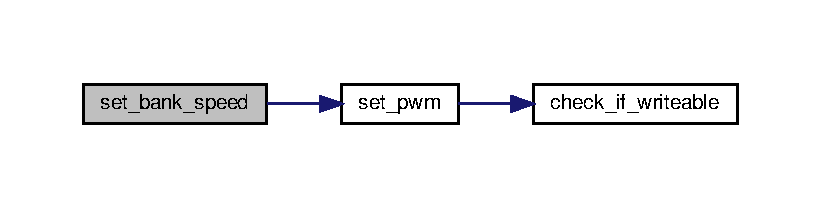
\includegraphics[width=350pt]{controller_8h_a79cb74a64d9173f1412a2b261d7ac82f_cgraph}
\end{center}
\end{figure}
\mbox{\Hypertarget{controller_8h_a26016d59d4d9df342535c2af5439f3c6}\label{controller_8h_a26016d59d4d9df342535c2af5439f3c6}} 
\index{controller.\+h@{controller.\+h}!tracking\+\_\+signal\+\_\+value@{tracking\+\_\+signal\+\_\+value}}
\index{tracking\+\_\+signal\+\_\+value@{tracking\+\_\+signal\+\_\+value}!controller.\+h@{controller.\+h}}
\subsubsection{\texorpdfstring{tracking\+\_\+signal\+\_\+value()}{tracking\_signal\_value()}}
{\footnotesize\ttfamily float tracking\+\_\+signal\+\_\+value (\begin{DoxyParamCaption}\item[{int}]{phi\+\_\+des,  }\item[{float}]{t,  }\item[{float}]{tr }\end{DoxyParamCaption})}



\subsection{Variable Documentation}
\mbox{\Hypertarget{controller_8h_ae3b00f80c9797211832566f1b2cff771}\label{controller_8h_ae3b00f80c9797211832566f1b2cff771}} 
\index{controller.\+h@{controller.\+h}!pid\+\_\+logger@{pid\+\_\+logger}}
\index{pid\+\_\+logger@{pid\+\_\+logger}!controller.\+h@{controller.\+h}}
\subsubsection{\texorpdfstring{pid\+\_\+logger}{pid\_logger}}
{\footnotesize\ttfamily \hyperlink{structLogger}{Logger}$\ast$ pid\+\_\+logger}


\hypertarget{error_8c}{}\section{error.\+c File Reference}
\label{error_8c}\index{error.\+c@{error.\+c}}
{\ttfamily \#include $<$stdlib.\+h$>$}\newline
{\ttfamily \#include $<$stdio.\+h$>$}\newline
{\ttfamily \#include \char`\"{}colors.\+h\char`\"{}}\newline
{\ttfamily \#include \char`\"{}error.\+h\char`\"{}}\newline
Include dependency graph for error.\+c\+:\nopagebreak
\begin{figure}[H]
\begin{center}
\leavevmode
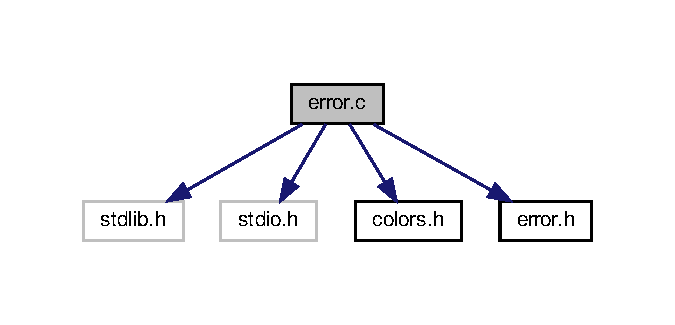
\includegraphics[width=324pt]{error_8c__incl}
\end{center}
\end{figure}
\subsection*{Functions}
\begin{DoxyCompactItemize}
\item 
void \hyperlink{error_8c_aa18dc63686c6269d22c7e878439391b1}{exit\+\_\+printing} (char $\ast$message, char code)
\end{DoxyCompactItemize}


\subsection{Function Documentation}
\mbox{\Hypertarget{error_8c_aa18dc63686c6269d22c7e878439391b1}\label{error_8c_aa18dc63686c6269d22c7e878439391b1}} 
\index{error.\+c@{error.\+c}!exit\+\_\+printing@{exit\+\_\+printing}}
\index{exit\+\_\+printing@{exit\+\_\+printing}!error.\+c@{error.\+c}}
\subsubsection{\texorpdfstring{exit\+\_\+printing()}{exit\_printing()}}
{\footnotesize\ttfamily void exit\+\_\+printing (\begin{DoxyParamCaption}\item[{char $\ast$}]{message,  }\item[{char}]{code }\end{DoxyParamCaption})}

Here is the caller graph for this function\+:\nopagebreak
\begin{figure}[H]
\begin{center}
\leavevmode
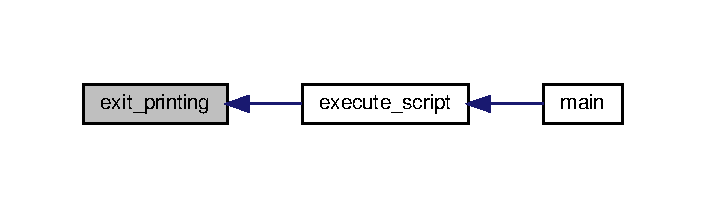
\includegraphics[width=339pt]{error_8c_aa18dc63686c6269d22c7e878439391b1_icgraph}
\end{center}
\end{figure}

\hypertarget{error_8h}{}\section{error.\+h File Reference}
\label{error_8h}\index{error.\+h@{error.\+h}}
This graph shows which files directly or indirectly include this file\+:\nopagebreak
\begin{figure}[H]
\begin{center}
\leavevmode
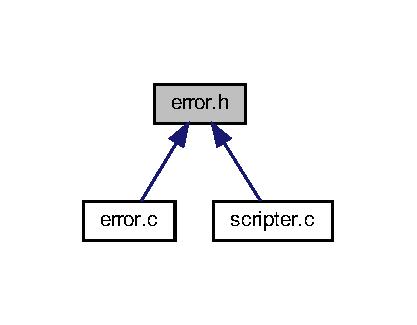
\includegraphics[width=200pt]{error_8h__dep__incl}
\end{center}
\end{figure}
\subsection*{Macros}
\begin{DoxyCompactItemize}
\item 
\#define \hyperlink{error_8h_a1415a4a1e5dec3e3a97ebb4a9a1db7dc}{E\+R\+R\+O\+R\+\_\+\+P\+R\+O\+G\+R\+A\+M\+M\+ER}~1
\item 
\#define \hyperlink{error_8h_a540d0b1a79f71518de58ee7473da10c3}{E\+R\+R\+O\+R\+\_\+\+O\+S\+\_\+\+F\+A\+I\+L\+U\+RE}~2
\item 
\#define \hyperlink{error_8h_a337812f79087f869224fa74d6367c419}{E\+R\+R\+O\+R\+\_\+\+L\+I\+B\+R\+A\+R\+Y\+\_\+\+F\+A\+I\+L\+U\+RE}~3
\end{DoxyCompactItemize}
\subsection*{Functions}
\begin{DoxyCompactItemize}
\item 
void \hyperlink{error_8h_aa18dc63686c6269d22c7e878439391b1}{exit\+\_\+printing} (char $\ast$message, char code)
\end{DoxyCompactItemize}


\subsection{Macro Definition Documentation}
\mbox{\Hypertarget{error_8h_a337812f79087f869224fa74d6367c419}\label{error_8h_a337812f79087f869224fa74d6367c419}} 
\index{error.\+h@{error.\+h}!E\+R\+R\+O\+R\+\_\+\+L\+I\+B\+R\+A\+R\+Y\+\_\+\+F\+A\+I\+L\+U\+RE@{E\+R\+R\+O\+R\+\_\+\+L\+I\+B\+R\+A\+R\+Y\+\_\+\+F\+A\+I\+L\+U\+RE}}
\index{E\+R\+R\+O\+R\+\_\+\+L\+I\+B\+R\+A\+R\+Y\+\_\+\+F\+A\+I\+L\+U\+RE@{E\+R\+R\+O\+R\+\_\+\+L\+I\+B\+R\+A\+R\+Y\+\_\+\+F\+A\+I\+L\+U\+RE}!error.\+h@{error.\+h}}
\subsubsection{\texorpdfstring{E\+R\+R\+O\+R\+\_\+\+L\+I\+B\+R\+A\+R\+Y\+\_\+\+F\+A\+I\+L\+U\+RE}{ERROR\_LIBRARY\_FAILURE}}
{\footnotesize\ttfamily \#define E\+R\+R\+O\+R\+\_\+\+L\+I\+B\+R\+A\+R\+Y\+\_\+\+F\+A\+I\+L\+U\+RE~3}

\mbox{\Hypertarget{error_8h_a540d0b1a79f71518de58ee7473da10c3}\label{error_8h_a540d0b1a79f71518de58ee7473da10c3}} 
\index{error.\+h@{error.\+h}!E\+R\+R\+O\+R\+\_\+\+O\+S\+\_\+\+F\+A\+I\+L\+U\+RE@{E\+R\+R\+O\+R\+\_\+\+O\+S\+\_\+\+F\+A\+I\+L\+U\+RE}}
\index{E\+R\+R\+O\+R\+\_\+\+O\+S\+\_\+\+F\+A\+I\+L\+U\+RE@{E\+R\+R\+O\+R\+\_\+\+O\+S\+\_\+\+F\+A\+I\+L\+U\+RE}!error.\+h@{error.\+h}}
\subsubsection{\texorpdfstring{E\+R\+R\+O\+R\+\_\+\+O\+S\+\_\+\+F\+A\+I\+L\+U\+RE}{ERROR\_OS\_FAILURE}}
{\footnotesize\ttfamily \#define E\+R\+R\+O\+R\+\_\+\+O\+S\+\_\+\+F\+A\+I\+L\+U\+RE~2}

\mbox{\Hypertarget{error_8h_a1415a4a1e5dec3e3a97ebb4a9a1db7dc}\label{error_8h_a1415a4a1e5dec3e3a97ebb4a9a1db7dc}} 
\index{error.\+h@{error.\+h}!E\+R\+R\+O\+R\+\_\+\+P\+R\+O\+G\+R\+A\+M\+M\+ER@{E\+R\+R\+O\+R\+\_\+\+P\+R\+O\+G\+R\+A\+M\+M\+ER}}
\index{E\+R\+R\+O\+R\+\_\+\+P\+R\+O\+G\+R\+A\+M\+M\+ER@{E\+R\+R\+O\+R\+\_\+\+P\+R\+O\+G\+R\+A\+M\+M\+ER}!error.\+h@{error.\+h}}
\subsubsection{\texorpdfstring{E\+R\+R\+O\+R\+\_\+\+P\+R\+O\+G\+R\+A\+M\+M\+ER}{ERROR\_PROGRAMMER}}
{\footnotesize\ttfamily \#define E\+R\+R\+O\+R\+\_\+\+P\+R\+O\+G\+R\+A\+M\+M\+ER~1}



\subsection{Function Documentation}
\mbox{\Hypertarget{error_8h_aa18dc63686c6269d22c7e878439391b1}\label{error_8h_aa18dc63686c6269d22c7e878439391b1}} 
\index{error.\+h@{error.\+h}!exit\+\_\+printing@{exit\+\_\+printing}}
\index{exit\+\_\+printing@{exit\+\_\+printing}!error.\+h@{error.\+h}}
\subsubsection{\texorpdfstring{exit\+\_\+printing()}{exit\_printing()}}
{\footnotesize\ttfamily void exit\+\_\+printing (\begin{DoxyParamCaption}\item[{char $\ast$}]{message,  }\item[{char}]{code }\end{DoxyParamCaption})}

Here is the caller graph for this function\+:\nopagebreak
\begin{figure}[H]
\begin{center}
\leavevmode
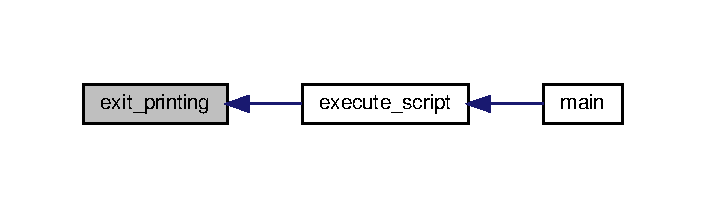
\includegraphics[width=339pt]{error_8h_aa18dc63686c6269d22c7e878439391b1_icgraph}
\end{center}
\end{figure}

\hypertarget{femta_8c}{}\section{femta.\+c File Reference}
\label{femta_8c}\index{femta.\+c@{femta.\+c}}
{\ttfamily \#include $<$stdbool.\+h$>$}\newline
{\ttfamily \#include $<$pthread.\+h$>$}\newline
{\ttfamily \#include $<$stdlib.\+h$>$}\newline
{\ttfamily \#include $<$pigpio.\+h$>$}\newline
{\ttfamily \#include $<$unistd.\+h$>$}\newline
{\ttfamily \#include $<$stdio.\+h$>$}\newline
{\ttfamily \#include \char`\"{}femta.\+h\char`\"{}}\newline
{\ttfamily \#include \char`\"{}i2c-\/interface.\+h\char`\"{}}\newline
{\ttfamily \#include \char`\"{}temperature-\/monitoring.\+h\char`\"{}}\newline
{\ttfamily \#include \char`\"{}graphics.\+h\char`\"{}}\newline
{\ttfamily \#include \char`\"{}selector.\+h\char`\"{}}\newline
{\ttfamily \#include \char`\"{}scripter.\+h\char`\"{}}\newline
{\ttfamily \#include \char`\"{}logger.\+h\char`\"{}}\newline
{\ttfamily \#include \char`\"{}colors.\+h\char`\"{}}\newline
Include dependency graph for femta.\+c\+:
\nopagebreak
\begin{figure}[H]
\begin{center}
\leavevmode
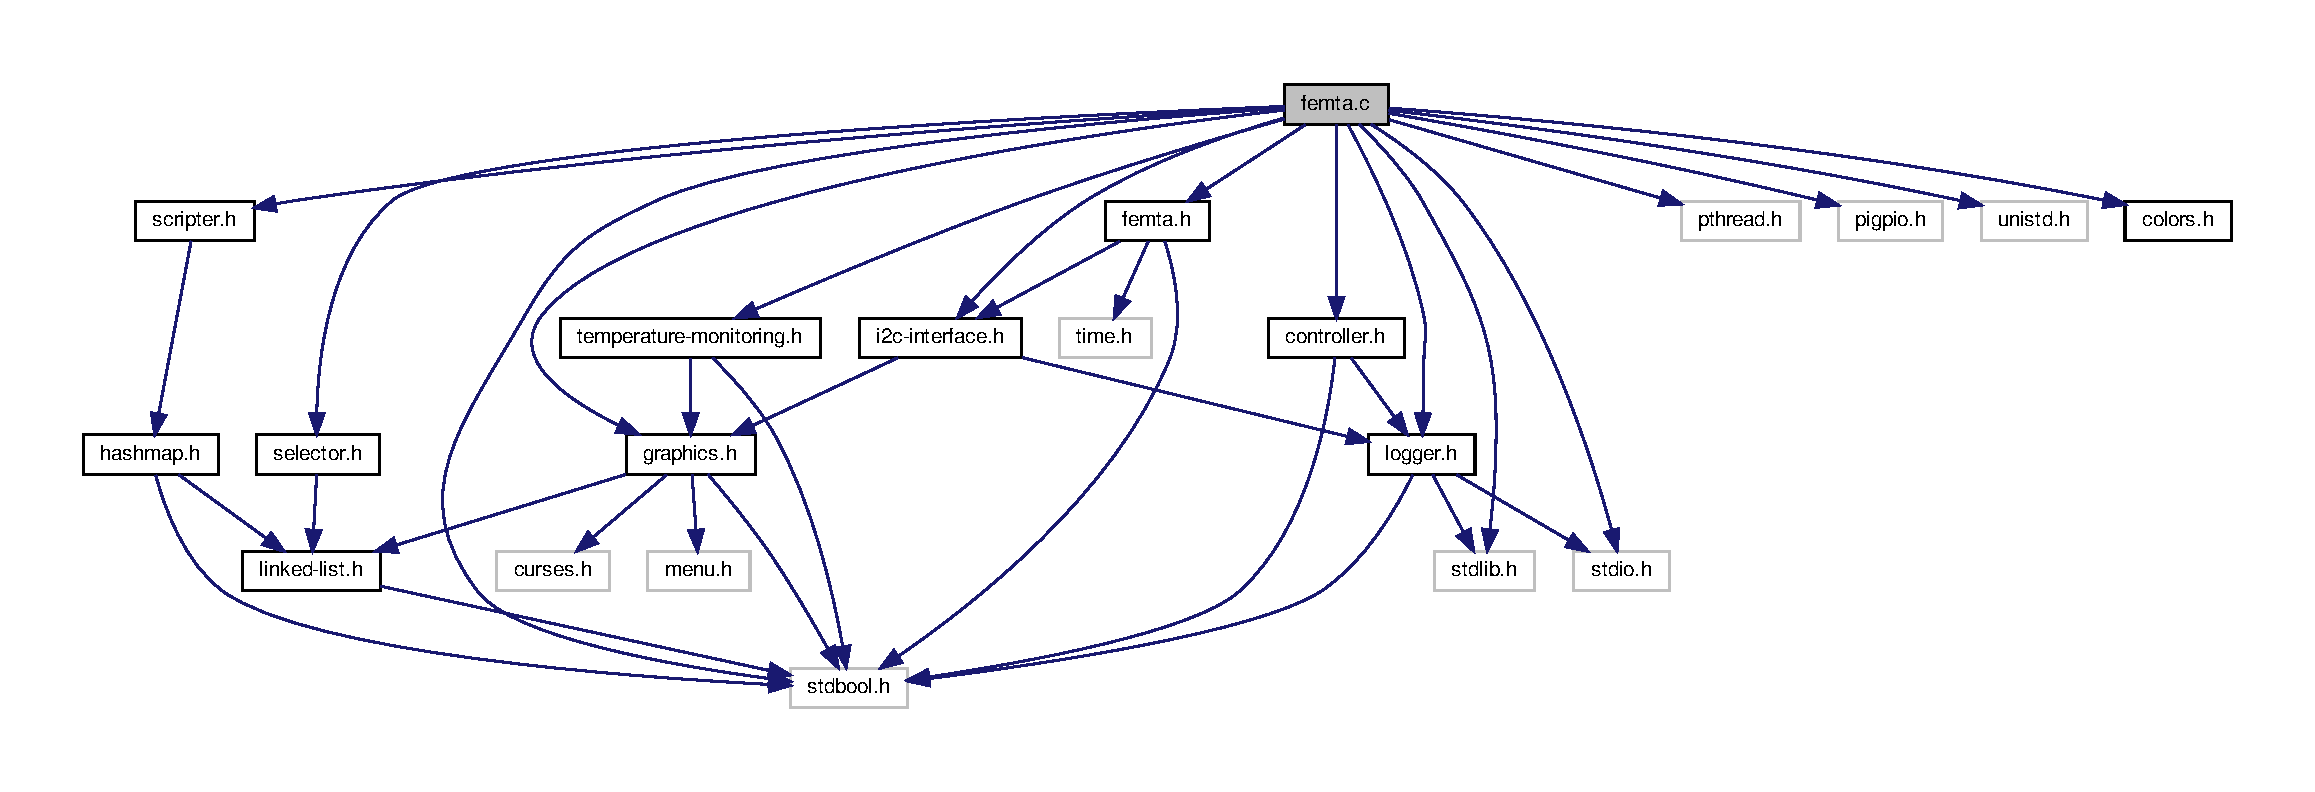
\includegraphics[width=350pt]{femta_8c__incl}
\end{center}
\end{figure}
\subsection*{Macros}
\begin{DoxyCompactItemize}
\item 
\#define \hyperlink{femta_8c_a52ede00c016989d352fbe071b104fddf}{N\+U\+M\+B\+E\+R\+\_\+\+O\+F\+\_\+\+M\+O\+D\+U\+L\+ES}~3
\item 
\#define \hyperlink{femta_8c_ab2d66e2cf934380faec387170c8192fb}{I2\+C\+\_\+\+S\+T\+A\+TE}~2
\item 
\#define \hyperlink{femta_8c_a30e07560cc19679bdfd1a4a0f375dcce}{U\+A\+R\+T\+\_\+\+S\+T\+A\+TE}~3
\end{DoxyCompactItemize}
\subsection*{Functions}
\begin{DoxyCompactItemize}
\item 
void \hyperlink{femta_8c_aff48f29e1c09dc2ca483addcf10af1fe}{initialize\+\_\+pin} (\hyperlink{structpin}{pin} $\ast$initialent, char logical, char physical, short state)
\item 
void \hyperlink{femta_8c_a8ecd8ad82265b8157b5c24ba269bf362}{initialize\+\_\+satellite} ()
\item 
void \hyperlink{femta_8c_a65b2dadc0411e43874ec8ed7f73bc62a}{print\+\_\+configuration} ()
\item 
void \hyperlink{femta_8c_a0fdde14054e696827c93273c03eb27aa}{terminate\+\_\+satellite} ()
\item 
void \hyperlink{femta_8c_a38759a3aa9cf6e83e88637bb2554cf42}{check\+\_\+if\+\_\+writeable} (\hyperlink{structpin}{pin} $\ast$p)
\item 
void \hyperlink{femta_8c_a9ee4f48eac43d3ba2da89c2755303f0c}{check\+\_\+if\+\_\+readable} (\hyperlink{structpin}{pin} $\ast$p)
\item 
char \hyperlink{femta_8c_ae27f4be41932fc0a949e878d9c43baea}{read\+\_\+voltage} (\hyperlink{structpin}{pin} $\ast$p)
\item 
void \hyperlink{femta_8c_add8fcf74e11d6f54778931df2410cf3a}{set\+\_\+voltage} (\hyperlink{structpin}{pin} $\ast$p, char voltage)
\item 
void \hyperlink{femta_8c_ab77890d508b0b089793017f183a470cd}{set\+\_\+pwm} (\hyperlink{structpin}{pin} $\ast$p, unsigned char duty\+\_\+cycle)
\item 
int \hyperlink{femta_8c_ae66f6b31b5ad750f1fe042a706a4e3d4}{main} ()
\end{DoxyCompactItemize}


\subsection{Macro Definition Documentation}
\mbox{\Hypertarget{femta_8c_ab2d66e2cf934380faec387170c8192fb}\label{femta_8c_ab2d66e2cf934380faec387170c8192fb}} 
\index{femta.\+c@{femta.\+c}!I2\+C\+\_\+\+S\+T\+A\+TE@{I2\+C\+\_\+\+S\+T\+A\+TE}}
\index{I2\+C\+\_\+\+S\+T\+A\+TE@{I2\+C\+\_\+\+S\+T\+A\+TE}!femta.\+c@{femta.\+c}}
\subsubsection{\texorpdfstring{I2\+C\+\_\+\+S\+T\+A\+TE}{I2C\_STATE}}
{\footnotesize\ttfamily \#define I2\+C\+\_\+\+S\+T\+A\+TE~2}

\mbox{\Hypertarget{femta_8c_a52ede00c016989d352fbe071b104fddf}\label{femta_8c_a52ede00c016989d352fbe071b104fddf}} 
\index{femta.\+c@{femta.\+c}!N\+U\+M\+B\+E\+R\+\_\+\+O\+F\+\_\+\+M\+O\+D\+U\+L\+ES@{N\+U\+M\+B\+E\+R\+\_\+\+O\+F\+\_\+\+M\+O\+D\+U\+L\+ES}}
\index{N\+U\+M\+B\+E\+R\+\_\+\+O\+F\+\_\+\+M\+O\+D\+U\+L\+ES@{N\+U\+M\+B\+E\+R\+\_\+\+O\+F\+\_\+\+M\+O\+D\+U\+L\+ES}!femta.\+c@{femta.\+c}}
\subsubsection{\texorpdfstring{N\+U\+M\+B\+E\+R\+\_\+\+O\+F\+\_\+\+M\+O\+D\+U\+L\+ES}{NUMBER\_OF\_MODULES}}
{\footnotesize\ttfamily \#define N\+U\+M\+B\+E\+R\+\_\+\+O\+F\+\_\+\+M\+O\+D\+U\+L\+ES~3}

\mbox{\Hypertarget{femta_8c_a30e07560cc19679bdfd1a4a0f375dcce}\label{femta_8c_a30e07560cc19679bdfd1a4a0f375dcce}} 
\index{femta.\+c@{femta.\+c}!U\+A\+R\+T\+\_\+\+S\+T\+A\+TE@{U\+A\+R\+T\+\_\+\+S\+T\+A\+TE}}
\index{U\+A\+R\+T\+\_\+\+S\+T\+A\+TE@{U\+A\+R\+T\+\_\+\+S\+T\+A\+TE}!femta.\+c@{femta.\+c}}
\subsubsection{\texorpdfstring{U\+A\+R\+T\+\_\+\+S\+T\+A\+TE}{UART\_STATE}}
{\footnotesize\ttfamily \#define U\+A\+R\+T\+\_\+\+S\+T\+A\+TE~3}



\subsection{Function Documentation}
\mbox{\Hypertarget{femta_8c_a9ee4f48eac43d3ba2da89c2755303f0c}\label{femta_8c_a9ee4f48eac43d3ba2da89c2755303f0c}} 
\index{femta.\+c@{femta.\+c}!check\+\_\+if\+\_\+readable@{check\+\_\+if\+\_\+readable}}
\index{check\+\_\+if\+\_\+readable@{check\+\_\+if\+\_\+readable}!femta.\+c@{femta.\+c}}
\subsubsection{\texorpdfstring{check\+\_\+if\+\_\+readable()}{check\_if\_readable()}}
{\footnotesize\ttfamily void check\+\_\+if\+\_\+readable (\begin{DoxyParamCaption}\item[{\hyperlink{structpin}{pin} $\ast$}]{p }\end{DoxyParamCaption})}

Here is the caller graph for this function\+:
\nopagebreak
\begin{figure}[H]
\begin{center}
\leavevmode
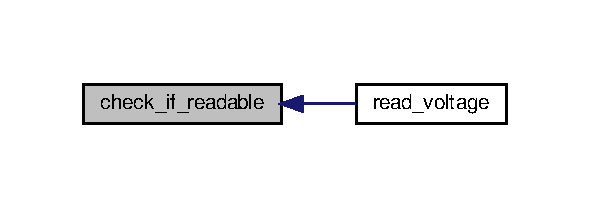
\includegraphics[width=283pt]{femta_8c_a9ee4f48eac43d3ba2da89c2755303f0c_icgraph}
\end{center}
\end{figure}
\mbox{\Hypertarget{femta_8c_a38759a3aa9cf6e83e88637bb2554cf42}\label{femta_8c_a38759a3aa9cf6e83e88637bb2554cf42}} 
\index{femta.\+c@{femta.\+c}!check\+\_\+if\+\_\+writeable@{check\+\_\+if\+\_\+writeable}}
\index{check\+\_\+if\+\_\+writeable@{check\+\_\+if\+\_\+writeable}!femta.\+c@{femta.\+c}}
\subsubsection{\texorpdfstring{check\+\_\+if\+\_\+writeable()}{check\_if\_writeable()}}
{\footnotesize\ttfamily void check\+\_\+if\+\_\+writeable (\begin{DoxyParamCaption}\item[{\hyperlink{structpin}{pin} $\ast$}]{p }\end{DoxyParamCaption})}

Here is the caller graph for this function\+:
\nopagebreak
\begin{figure}[H]
\begin{center}
\leavevmode
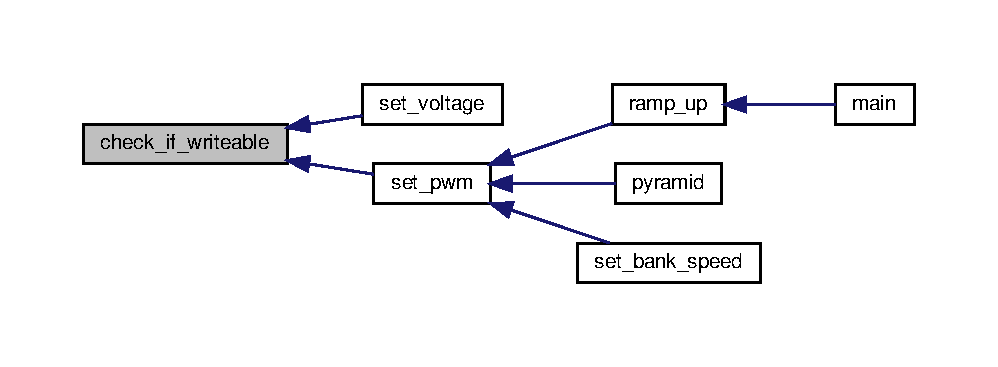
\includegraphics[width=281pt]{femta_8c_a38759a3aa9cf6e83e88637bb2554cf42_icgraph}
\end{center}
\end{figure}
\mbox{\Hypertarget{femta_8c_aff48f29e1c09dc2ca483addcf10af1fe}\label{femta_8c_aff48f29e1c09dc2ca483addcf10af1fe}} 
\index{femta.\+c@{femta.\+c}!initialize\+\_\+pin@{initialize\+\_\+pin}}
\index{initialize\+\_\+pin@{initialize\+\_\+pin}!femta.\+c@{femta.\+c}}
\subsubsection{\texorpdfstring{initialize\+\_\+pin()}{initialize\_pin()}}
{\footnotesize\ttfamily void initialize\+\_\+pin (\begin{DoxyParamCaption}\item[{\hyperlink{structpin}{pin} $\ast$}]{initialent,  }\item[{char}]{logical,  }\item[{char}]{physical,  }\item[{short}]{state }\end{DoxyParamCaption})}

Here is the caller graph for this function\+:
\nopagebreak
\begin{figure}[H]
\begin{center}
\leavevmode
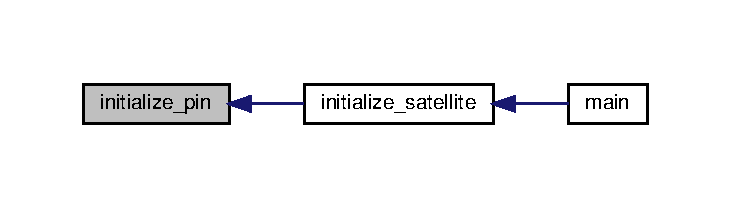
\includegraphics[width=350pt]{femta_8c_aff48f29e1c09dc2ca483addcf10af1fe_icgraph}
\end{center}
\end{figure}
\mbox{\Hypertarget{femta_8c_a8ecd8ad82265b8157b5c24ba269bf362}\label{femta_8c_a8ecd8ad82265b8157b5c24ba269bf362}} 
\index{femta.\+c@{femta.\+c}!initialize\+\_\+satellite@{initialize\+\_\+satellite}}
\index{initialize\+\_\+satellite@{initialize\+\_\+satellite}!femta.\+c@{femta.\+c}}
\subsubsection{\texorpdfstring{initialize\+\_\+satellite()}{initialize\_satellite()}}
{\footnotesize\ttfamily void initialize\+\_\+satellite (\begin{DoxyParamCaption}{ }\end{DoxyParamCaption})}

Here is the call graph for this function\+:
\nopagebreak
\begin{figure}[H]
\begin{center}
\leavevmode
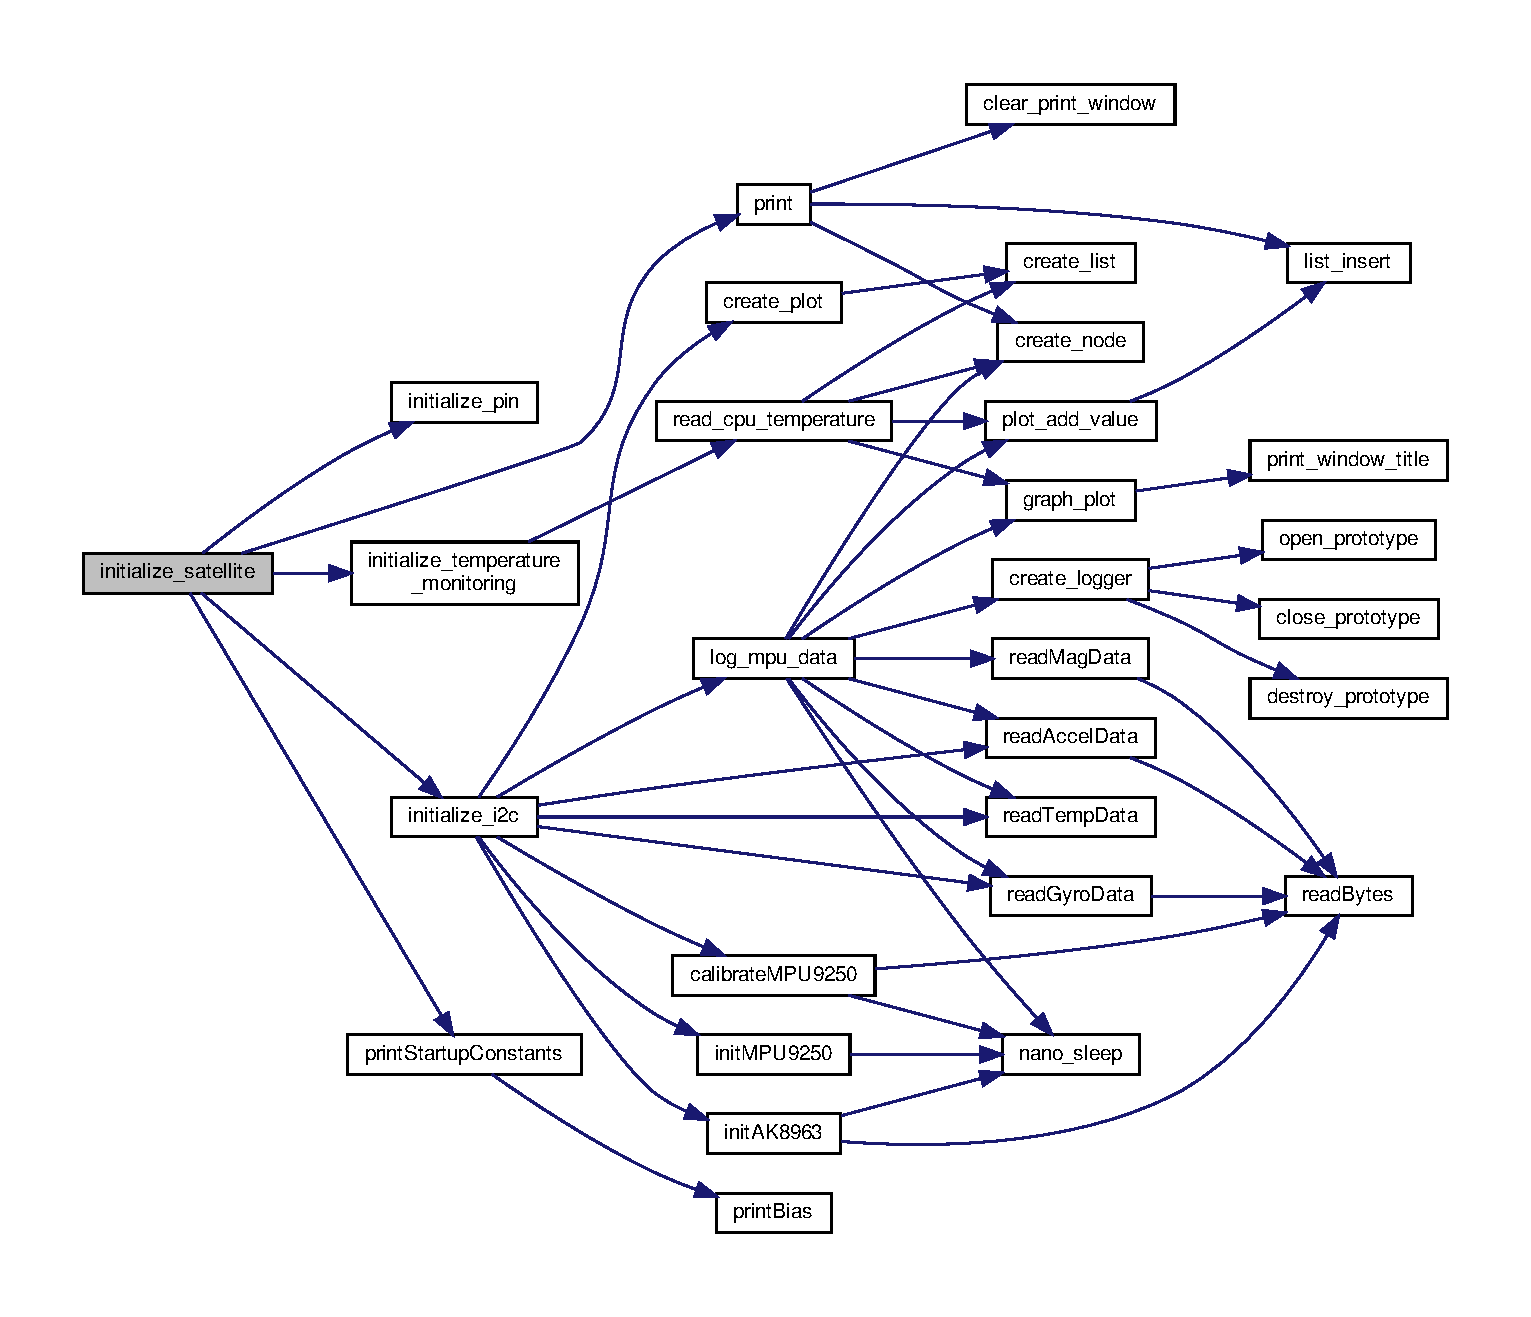
\includegraphics[width=350pt]{femta_8c_a8ecd8ad82265b8157b5c24ba269bf362_cgraph}
\end{center}
\end{figure}
Here is the caller graph for this function\+:
\nopagebreak
\begin{figure}[H]
\begin{center}
\leavevmode
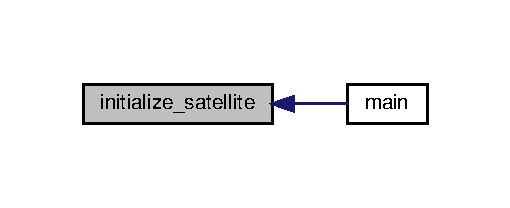
\includegraphics[width=245pt]{femta_8c_a8ecd8ad82265b8157b5c24ba269bf362_icgraph}
\end{center}
\end{figure}
\mbox{\Hypertarget{femta_8c_ae66f6b31b5ad750f1fe042a706a4e3d4}\label{femta_8c_ae66f6b31b5ad750f1fe042a706a4e3d4}} 
\index{femta.\+c@{femta.\+c}!main@{main}}
\index{main@{main}!femta.\+c@{femta.\+c}}
\subsubsection{\texorpdfstring{main()}{main()}}
{\footnotesize\ttfamily int main (\begin{DoxyParamCaption}{ }\end{DoxyParamCaption})}

Here is the call graph for this function\+:
\nopagebreak
\begin{figure}[H]
\begin{center}
\leavevmode
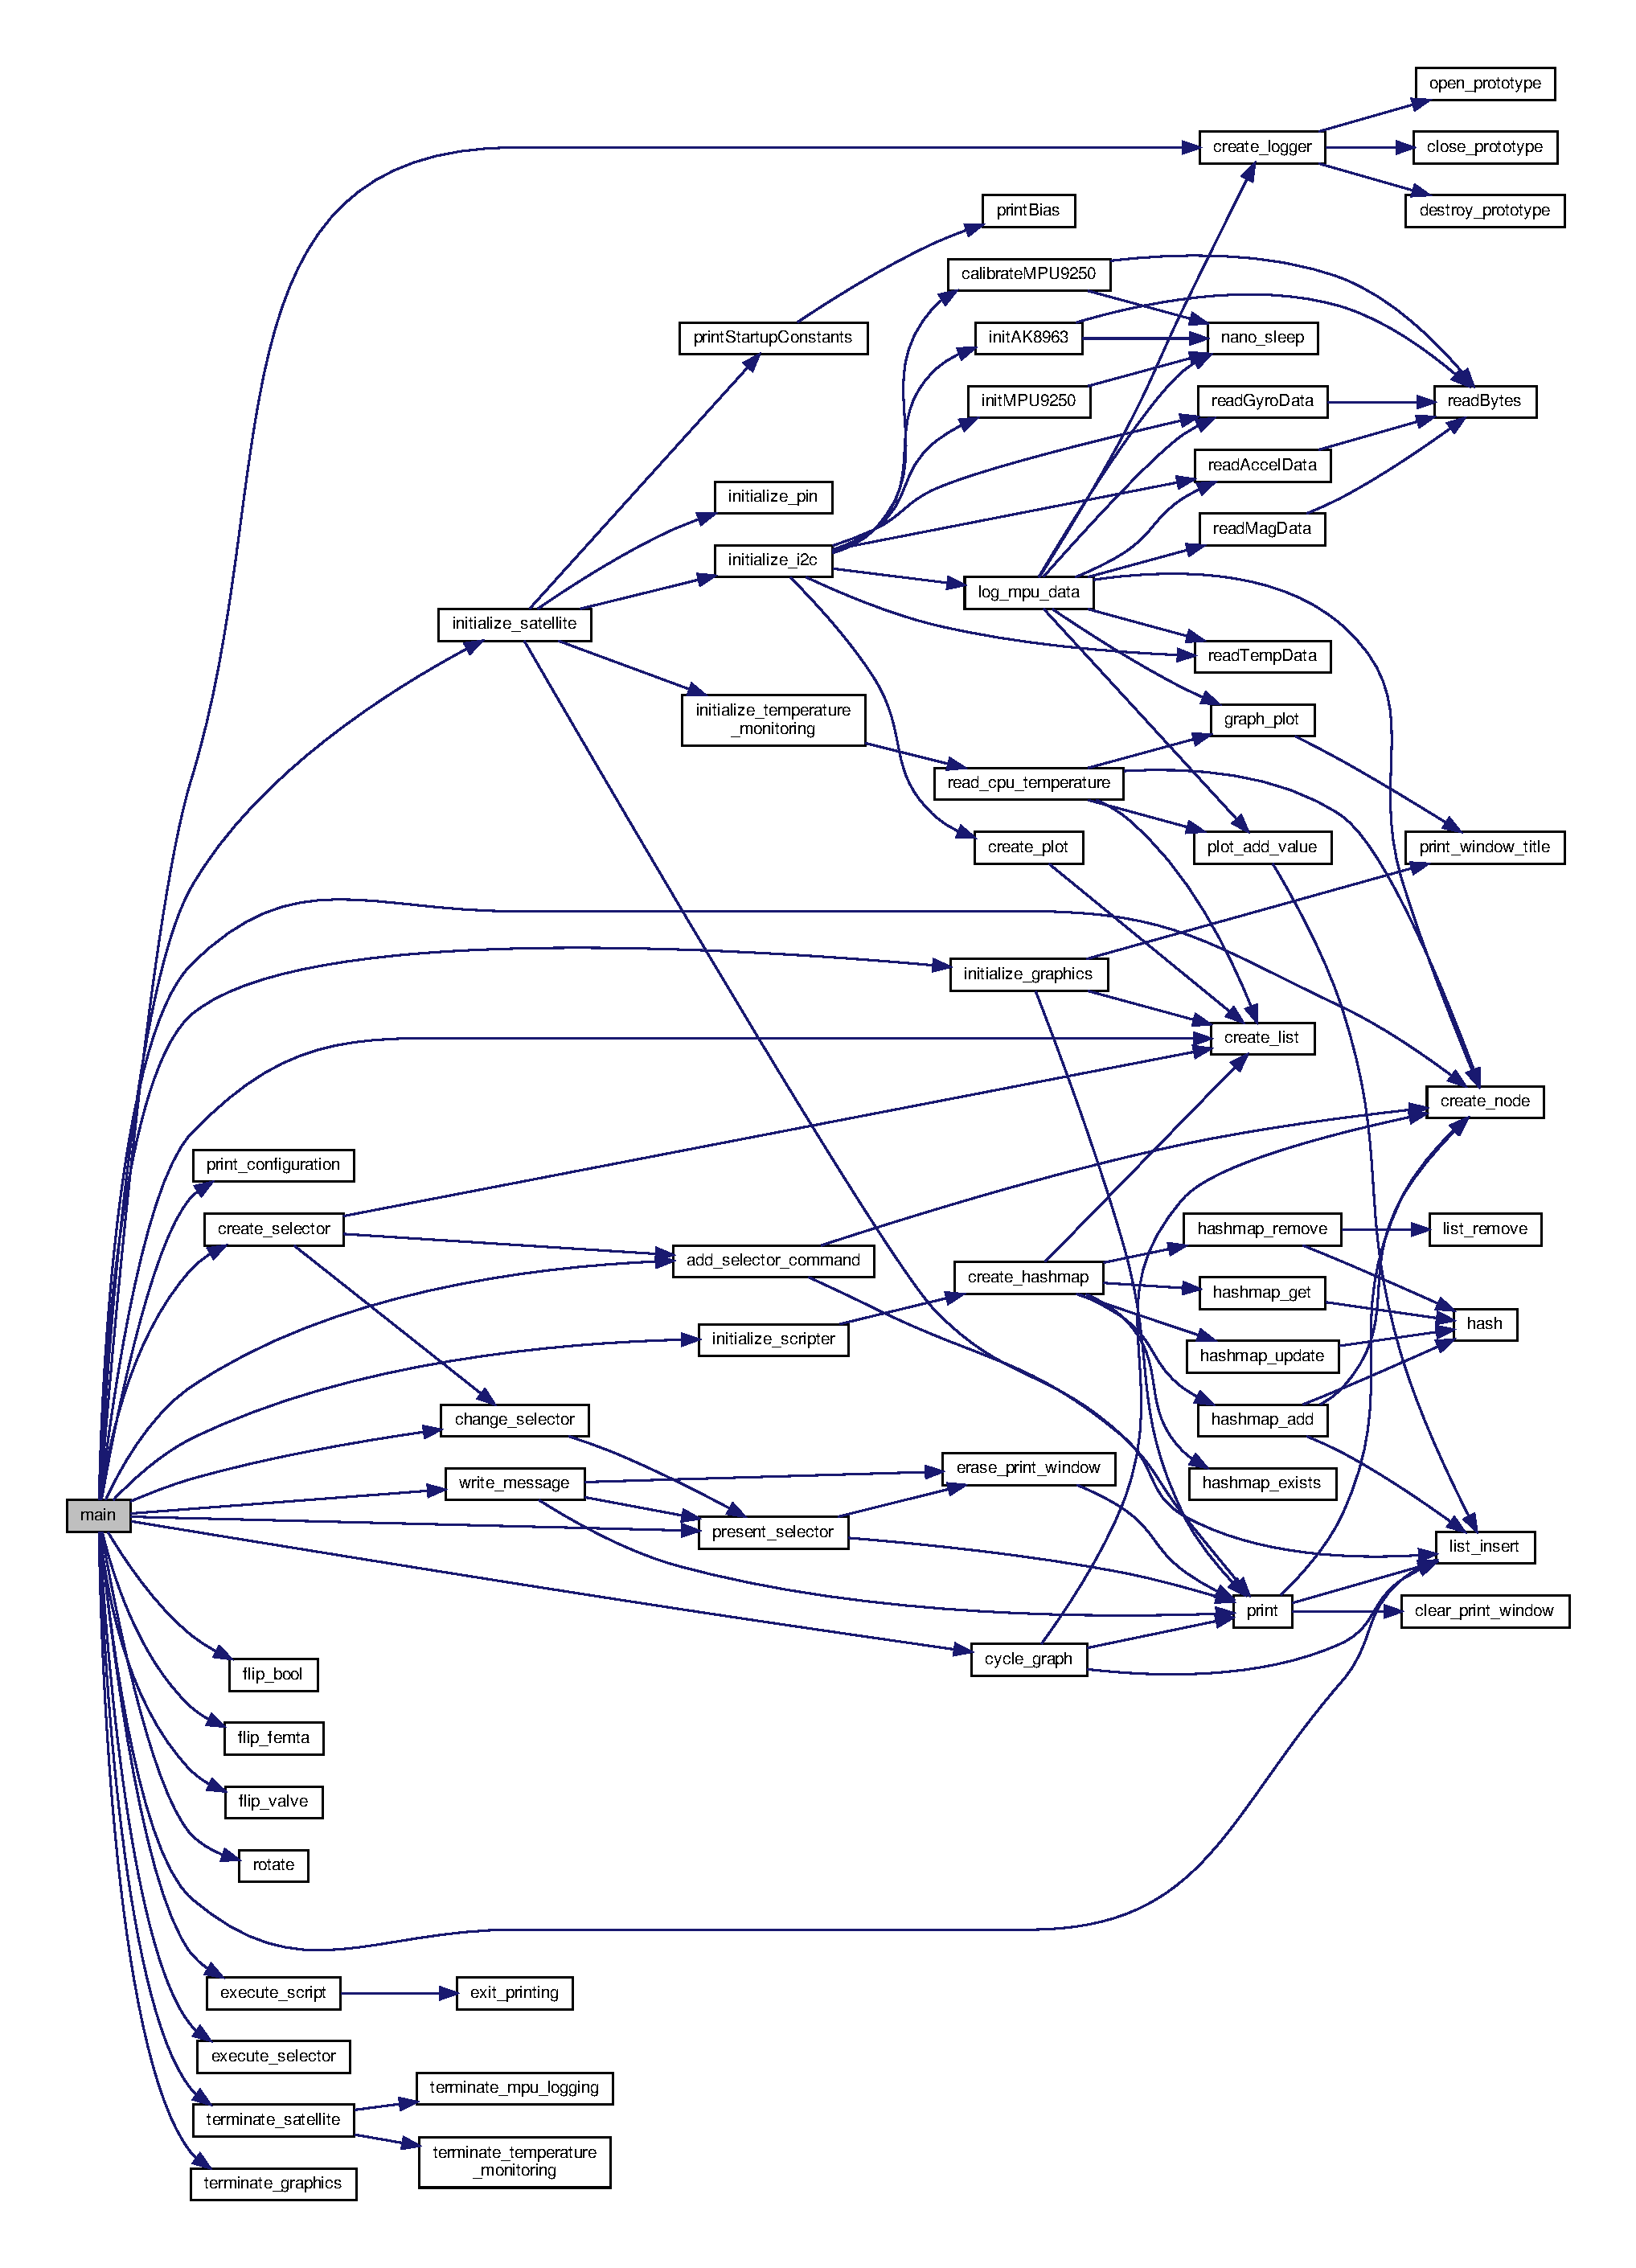
\includegraphics[width=350pt]{femta_8c_ae66f6b31b5ad750f1fe042a706a4e3d4_cgraph}
\end{center}
\end{figure}
\mbox{\Hypertarget{femta_8c_a65b2dadc0411e43874ec8ed7f73bc62a}\label{femta_8c_a65b2dadc0411e43874ec8ed7f73bc62a}} 
\index{femta.\+c@{femta.\+c}!print\+\_\+configuration@{print\+\_\+configuration}}
\index{print\+\_\+configuration@{print\+\_\+configuration}!femta.\+c@{femta.\+c}}
\subsubsection{\texorpdfstring{print\+\_\+configuration()}{print\_configuration()}}
{\footnotesize\ttfamily void print\+\_\+configuration (\begin{DoxyParamCaption}{ }\end{DoxyParamCaption})}

Here is the caller graph for this function\+:
\nopagebreak
\begin{figure}[H]
\begin{center}
\leavevmode
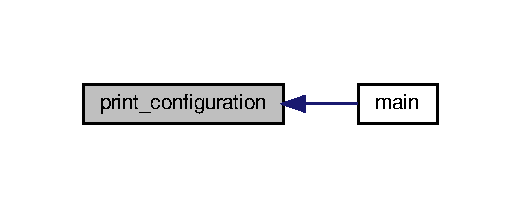
\includegraphics[width=250pt]{femta_8c_a65b2dadc0411e43874ec8ed7f73bc62a_icgraph}
\end{center}
\end{figure}
\mbox{\Hypertarget{femta_8c_ae27f4be41932fc0a949e878d9c43baea}\label{femta_8c_ae27f4be41932fc0a949e878d9c43baea}} 
\index{femta.\+c@{femta.\+c}!read\+\_\+voltage@{read\+\_\+voltage}}
\index{read\+\_\+voltage@{read\+\_\+voltage}!femta.\+c@{femta.\+c}}
\subsubsection{\texorpdfstring{read\+\_\+voltage()}{read\_voltage()}}
{\footnotesize\ttfamily char read\+\_\+voltage (\begin{DoxyParamCaption}\item[{\hyperlink{structpin}{pin} $\ast$}]{p }\end{DoxyParamCaption})}

Here is the call graph for this function\+:
\nopagebreak
\begin{figure}[H]
\begin{center}
\leavevmode
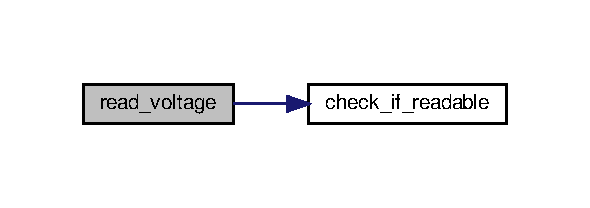
\includegraphics[width=283pt]{femta_8c_ae27f4be41932fc0a949e878d9c43baea_cgraph}
\end{center}
\end{figure}
\mbox{\Hypertarget{femta_8c_ab77890d508b0b089793017f183a470cd}\label{femta_8c_ab77890d508b0b089793017f183a470cd}} 
\index{femta.\+c@{femta.\+c}!set\+\_\+pwm@{set\+\_\+pwm}}
\index{set\+\_\+pwm@{set\+\_\+pwm}!femta.\+c@{femta.\+c}}
\subsubsection{\texorpdfstring{set\+\_\+pwm()}{set\_pwm()}}
{\footnotesize\ttfamily void set\+\_\+pwm (\begin{DoxyParamCaption}\item[{\hyperlink{structpin}{pin} $\ast$}]{p,  }\item[{unsigned char}]{duty\+\_\+cycle }\end{DoxyParamCaption})}

Here is the call graph for this function\+:
\nopagebreak
\begin{figure}[H]
\begin{center}
\leavevmode
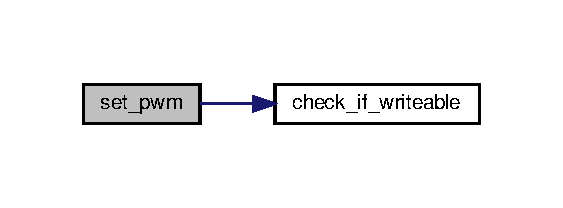
\includegraphics[width=270pt]{femta_8c_ab77890d508b0b089793017f183a470cd_cgraph}
\end{center}
\end{figure}
\mbox{\Hypertarget{femta_8c_add8fcf74e11d6f54778931df2410cf3a}\label{femta_8c_add8fcf74e11d6f54778931df2410cf3a}} 
\index{femta.\+c@{femta.\+c}!set\+\_\+voltage@{set\+\_\+voltage}}
\index{set\+\_\+voltage@{set\+\_\+voltage}!femta.\+c@{femta.\+c}}
\subsubsection{\texorpdfstring{set\+\_\+voltage()}{set\_voltage()}}
{\footnotesize\ttfamily void set\+\_\+voltage (\begin{DoxyParamCaption}\item[{\hyperlink{structpin}{pin} $\ast$}]{p,  }\item[{char}]{voltage }\end{DoxyParamCaption})}

Here is the call graph for this function\+:
\nopagebreak
\begin{figure}[H]
\begin{center}
\leavevmode
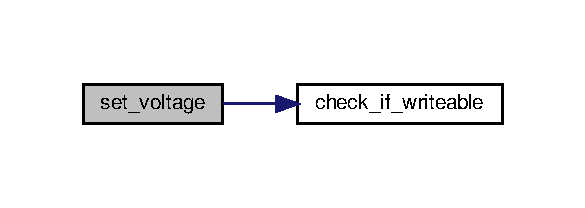
\includegraphics[width=281pt]{femta_8c_add8fcf74e11d6f54778931df2410cf3a_cgraph}
\end{center}
\end{figure}
\mbox{\Hypertarget{femta_8c_a0fdde14054e696827c93273c03eb27aa}\label{femta_8c_a0fdde14054e696827c93273c03eb27aa}} 
\index{femta.\+c@{femta.\+c}!terminate\+\_\+satellite@{terminate\+\_\+satellite}}
\index{terminate\+\_\+satellite@{terminate\+\_\+satellite}!femta.\+c@{femta.\+c}}
\subsubsection{\texorpdfstring{terminate\+\_\+satellite()}{terminate\_satellite()}}
{\footnotesize\ttfamily void terminate\+\_\+satellite (\begin{DoxyParamCaption}{ }\end{DoxyParamCaption})}

Here is the call graph for this function\+:
\nopagebreak
\begin{figure}[H]
\begin{center}
\leavevmode
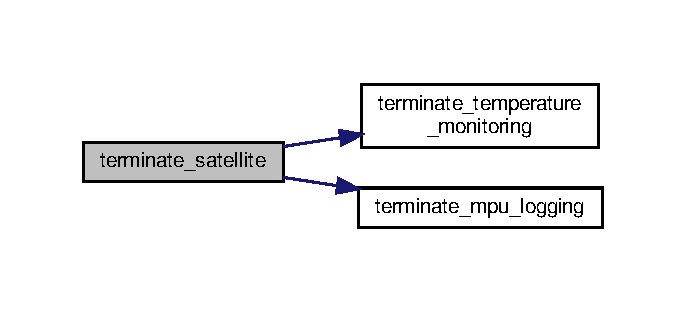
\includegraphics[width=329pt]{femta_8c_a0fdde14054e696827c93273c03eb27aa_cgraph}
\end{center}
\end{figure}
Here is the caller graph for this function\+:
\nopagebreak
\begin{figure}[H]
\begin{center}
\leavevmode
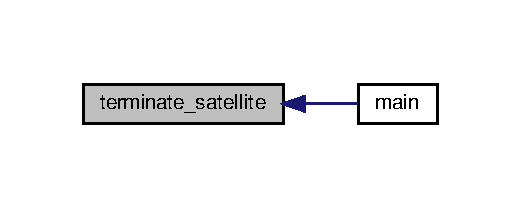
\includegraphics[width=250pt]{femta_8c_a0fdde14054e696827c93273c03eb27aa_icgraph}
\end{center}
\end{figure}

\hypertarget{femta_8h}{}\section{femta.\+h File Reference}
\label{femta_8h}\index{femta.\+h@{femta.\+h}}
{\ttfamily \#include $<$stdbool.\+h$>$}\newline
{\ttfamily \#include $<$time.\+h$>$}\newline
{\ttfamily \#include \char`\"{}i2c-\/interface.\+h\char`\"{}}\newline
Include dependency graph for femta.\+h\+:\nopagebreak
\begin{figure}[H]
\begin{center}
\leavevmode
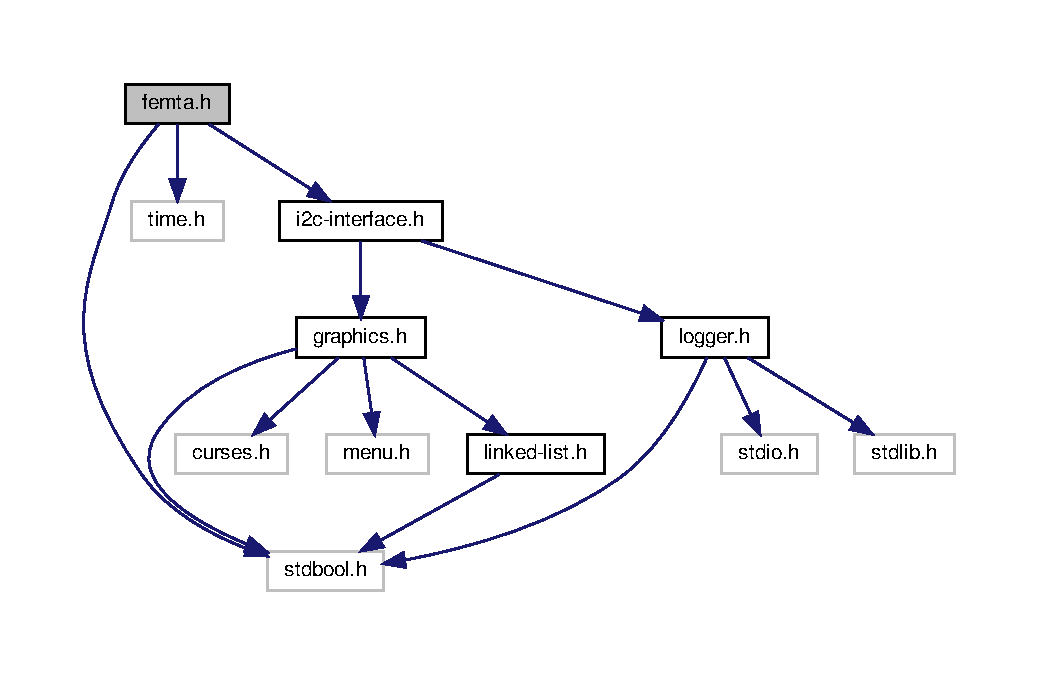
\includegraphics[width=350pt]{femta_8h__incl}
\end{center}
\end{figure}
This graph shows which files directly or indirectly include this file\+:
\nopagebreak
\begin{figure}[H]
\begin{center}
\leavevmode
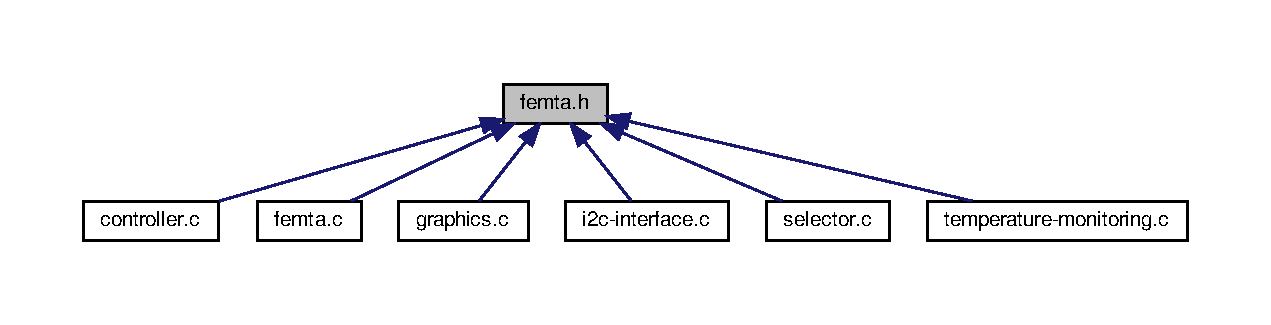
\includegraphics[width=350pt]{femta_8h__dep__incl}
\end{center}
\end{figure}
\subsection*{Classes}
\begin{DoxyCompactItemize}
\item 
struct \hyperlink{structpin}{pin}
\item 
struct \hyperlink{structmodule}{module}
\end{DoxyCompactItemize}
\subsection*{Typedefs}
\begin{DoxyCompactItemize}
\item 
typedef struct \hyperlink{structpin}{pin} \hyperlink{femta_8h_a2cc9367ff85ac26f1f3480522ed8b81b}{pin}
\item 
typedef struct \hyperlink{structI2C}{I2C} \hyperlink{femta_8h_a11fc462d06f4a1b3faa9ee895758cdcc}{I2C}
\item 
typedef struct \hyperlink{femta_8h_a13b3221f36ef9cb93c995303f10fed50}{U\+A\+RT} \hyperlink{femta_8h_a13b3221f36ef9cb93c995303f10fed50}{U\+A\+RT}
\item 
typedef struct \hyperlink{structmodule}{module} \hyperlink{femta_8h_af823706dd788a41282165a94f3a3d52c}{module}
\end{DoxyCompactItemize}
\subsection*{Functions}
\begin{DoxyCompactItemize}
\item 
void \hyperlink{femta_8h_add8fcf74e11d6f54778931df2410cf3a}{set\+\_\+voltage} (\hyperlink{structpin}{pin} $\ast$p, char voltage)
\item 
void \hyperlink{femta_8h_ab77890d508b0b089793017f183a470cd}{set\+\_\+pwm} (\hyperlink{structpin}{pin} $\ast$p, unsigned char duty\+\_\+cycle)
\end{DoxyCompactItemize}
\subsection*{Variables}
\begin{DoxyCompactItemize}
\item 
\hyperlink{structmodule}{module} $\ast$$\ast$ \hyperlink{femta_8h_a683045fff544d9aef3a4e19467ad8a0f}{modules}
\item 
\hyperlink{structmodule}{module} $\ast$ \hyperlink{femta_8h_a48d8b2f49274bf6f6ff62f773be3008f}{M\+PU}
\item 
\hyperlink{structmodule}{module} $\ast$ \hyperlink{femta_8h_a5391f686a31f8f821be08bf57774e4fe}{Valve}
\item 
\hyperlink{structmodule}{module} $\ast$ \hyperlink{femta_8h_ab98b7042e535dae4972a7e9a83dd773b}{F\+E\+M\+TA}
\item 
\hyperlink{structmodule}{module} $\ast$ \hyperlink{femta_8h_a96c523dc31e9e2892e26f20f3332ac89}{QB}
\item 
time\+\_\+t \hyperlink{femta_8h_ad20e89e0c86aa812dc3a8e2fb7b5777b}{start\+\_\+time}
\end{DoxyCompactItemize}


\subsection{Typedef Documentation}
\mbox{\Hypertarget{femta_8h_a11fc462d06f4a1b3faa9ee895758cdcc}\label{femta_8h_a11fc462d06f4a1b3faa9ee895758cdcc}} 
\index{femta.\+h@{femta.\+h}!I2C@{I2C}}
\index{I2C@{I2C}!femta.\+h@{femta.\+h}}
\subsubsection{\texorpdfstring{I2C}{I2C}}
{\footnotesize\ttfamily typedef struct \hyperlink{structI2C}{I2C} \hyperlink{structI2C}{I2C}}

\mbox{\Hypertarget{femta_8h_af823706dd788a41282165a94f3a3d52c}\label{femta_8h_af823706dd788a41282165a94f3a3d52c}} 
\index{femta.\+h@{femta.\+h}!module@{module}}
\index{module@{module}!femta.\+h@{femta.\+h}}
\subsubsection{\texorpdfstring{module}{module}}
{\footnotesize\ttfamily typedef struct \hyperlink{structmodule}{module}  \hyperlink{structmodule}{module}}

\mbox{\Hypertarget{femta_8h_a2cc9367ff85ac26f1f3480522ed8b81b}\label{femta_8h_a2cc9367ff85ac26f1f3480522ed8b81b}} 
\index{femta.\+h@{femta.\+h}!pin@{pin}}
\index{pin@{pin}!femta.\+h@{femta.\+h}}
\subsubsection{\texorpdfstring{pin}{pin}}
{\footnotesize\ttfamily typedef struct \hyperlink{structpin}{pin}  \hyperlink{structpin}{pin}}

\mbox{\Hypertarget{femta_8h_a13b3221f36ef9cb93c995303f10fed50}\label{femta_8h_a13b3221f36ef9cb93c995303f10fed50}} 
\index{femta.\+h@{femta.\+h}!U\+A\+RT@{U\+A\+RT}}
\index{U\+A\+RT@{U\+A\+RT}!femta.\+h@{femta.\+h}}
\subsubsection{\texorpdfstring{U\+A\+RT}{UART}}
{\footnotesize\ttfamily typedef struct \hyperlink{femta_8h_a13b3221f36ef9cb93c995303f10fed50}{U\+A\+RT} \hyperlink{femta_8h_a13b3221f36ef9cb93c995303f10fed50}{U\+A\+RT}}



\subsection{Function Documentation}
\mbox{\Hypertarget{femta_8h_ab77890d508b0b089793017f183a470cd}\label{femta_8h_ab77890d508b0b089793017f183a470cd}} 
\index{femta.\+h@{femta.\+h}!set\+\_\+pwm@{set\+\_\+pwm}}
\index{set\+\_\+pwm@{set\+\_\+pwm}!femta.\+h@{femta.\+h}}
\subsubsection{\texorpdfstring{set\+\_\+pwm()}{set\_pwm()}}
{\footnotesize\ttfamily void set\+\_\+pwm (\begin{DoxyParamCaption}\item[{\hyperlink{structpin}{pin} $\ast$}]{p,  }\item[{unsigned char}]{duty\+\_\+cycle }\end{DoxyParamCaption})}

Here is the call graph for this function\+:
\nopagebreak
\begin{figure}[H]
\begin{center}
\leavevmode
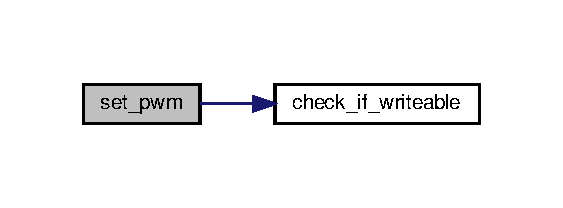
\includegraphics[width=270pt]{femta_8h_ab77890d508b0b089793017f183a470cd_cgraph}
\end{center}
\end{figure}
Here is the caller graph for this function\+:
\nopagebreak
\begin{figure}[H]
\begin{center}
\leavevmode
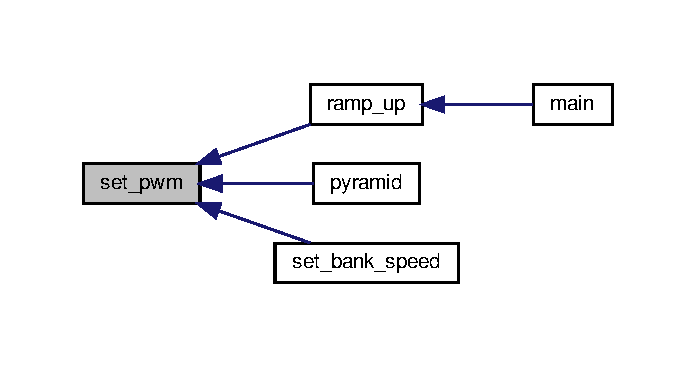
\includegraphics[width=334pt]{femta_8h_ab77890d508b0b089793017f183a470cd_icgraph}
\end{center}
\end{figure}
\mbox{\Hypertarget{femta_8h_add8fcf74e11d6f54778931df2410cf3a}\label{femta_8h_add8fcf74e11d6f54778931df2410cf3a}} 
\index{femta.\+h@{femta.\+h}!set\+\_\+voltage@{set\+\_\+voltage}}
\index{set\+\_\+voltage@{set\+\_\+voltage}!femta.\+h@{femta.\+h}}
\subsubsection{\texorpdfstring{set\+\_\+voltage()}{set\_voltage()}}
{\footnotesize\ttfamily void set\+\_\+voltage (\begin{DoxyParamCaption}\item[{\hyperlink{structpin}{pin} $\ast$}]{p,  }\item[{char}]{voltage }\end{DoxyParamCaption})}

Here is the call graph for this function\+:
\nopagebreak
\begin{figure}[H]
\begin{center}
\leavevmode
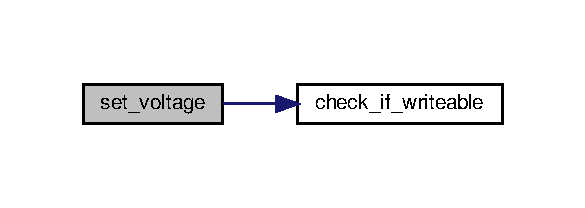
\includegraphics[width=281pt]{femta_8h_add8fcf74e11d6f54778931df2410cf3a_cgraph}
\end{center}
\end{figure}


\subsection{Variable Documentation}
\mbox{\Hypertarget{femta_8h_ab98b7042e535dae4972a7e9a83dd773b}\label{femta_8h_ab98b7042e535dae4972a7e9a83dd773b}} 
\index{femta.\+h@{femta.\+h}!F\+E\+M\+TA@{F\+E\+M\+TA}}
\index{F\+E\+M\+TA@{F\+E\+M\+TA}!femta.\+h@{femta.\+h}}
\subsubsection{\texorpdfstring{F\+E\+M\+TA}{FEMTA}}
{\footnotesize\ttfamily \hyperlink{structmodule}{module} $\ast$ F\+E\+M\+TA}

\mbox{\Hypertarget{femta_8h_a683045fff544d9aef3a4e19467ad8a0f}\label{femta_8h_a683045fff544d9aef3a4e19467ad8a0f}} 
\index{femta.\+h@{femta.\+h}!modules@{modules}}
\index{modules@{modules}!femta.\+h@{femta.\+h}}
\subsubsection{\texorpdfstring{modules}{modules}}
{\footnotesize\ttfamily \hyperlink{structmodule}{module}$\ast$$\ast$ modules}

\mbox{\Hypertarget{femta_8h_a48d8b2f49274bf6f6ff62f773be3008f}\label{femta_8h_a48d8b2f49274bf6f6ff62f773be3008f}} 
\index{femta.\+h@{femta.\+h}!M\+PU@{M\+PU}}
\index{M\+PU@{M\+PU}!femta.\+h@{femta.\+h}}
\subsubsection{\texorpdfstring{M\+PU}{MPU}}
{\footnotesize\ttfamily \hyperlink{structmodule}{module} $\ast$ M\+PU}

\mbox{\Hypertarget{femta_8h_a96c523dc31e9e2892e26f20f3332ac89}\label{femta_8h_a96c523dc31e9e2892e26f20f3332ac89}} 
\index{femta.\+h@{femta.\+h}!QB@{QB}}
\index{QB@{QB}!femta.\+h@{femta.\+h}}
\subsubsection{\texorpdfstring{QB}{QB}}
{\footnotesize\ttfamily \hyperlink{structmodule}{module} $\ast$ QB}

\mbox{\Hypertarget{femta_8h_ad20e89e0c86aa812dc3a8e2fb7b5777b}\label{femta_8h_ad20e89e0c86aa812dc3a8e2fb7b5777b}} 
\index{femta.\+h@{femta.\+h}!start\+\_\+time@{start\+\_\+time}}
\index{start\+\_\+time@{start\+\_\+time}!femta.\+h@{femta.\+h}}
\subsubsection{\texorpdfstring{start\+\_\+time}{start\_time}}
{\footnotesize\ttfamily time\+\_\+t start\+\_\+time}

\mbox{\Hypertarget{femta_8h_a5391f686a31f8f821be08bf57774e4fe}\label{femta_8h_a5391f686a31f8f821be08bf57774e4fe}} 
\index{femta.\+h@{femta.\+h}!Valve@{Valve}}
\index{Valve@{Valve}!femta.\+h@{femta.\+h}}
\subsubsection{\texorpdfstring{Valve}{Valve}}
{\footnotesize\ttfamily \hyperlink{structmodule}{module} $\ast$ Valve}


\hypertarget{graphics_8c}{}\section{graphics.\+c File Reference}
\label{graphics_8c}\index{graphics.\+c@{graphics.\+c}}
{\ttfamily \#include $<$stdlib.\+h$>$}\newline
{\ttfamily \#include $<$stdint.\+h$>$}\newline
{\ttfamily \#include $<$string.\+h$>$}\newline
{\ttfamily \#include $<$pigpio.\+h$>$}\newline
{\ttfamily \#include $<$curses.\+h$>$}\newline
{\ttfamily \#include $<$menu.\+h$>$}\newline
{\ttfamily \#include \char`\"{}graphics.\+h\char`\"{}}\newline
{\ttfamily \#include \char`\"{}femta.\+h\char`\"{}}\newline
Include dependency graph for graphics.\+c\+:
\nopagebreak
\begin{figure}[H]
\begin{center}
\leavevmode
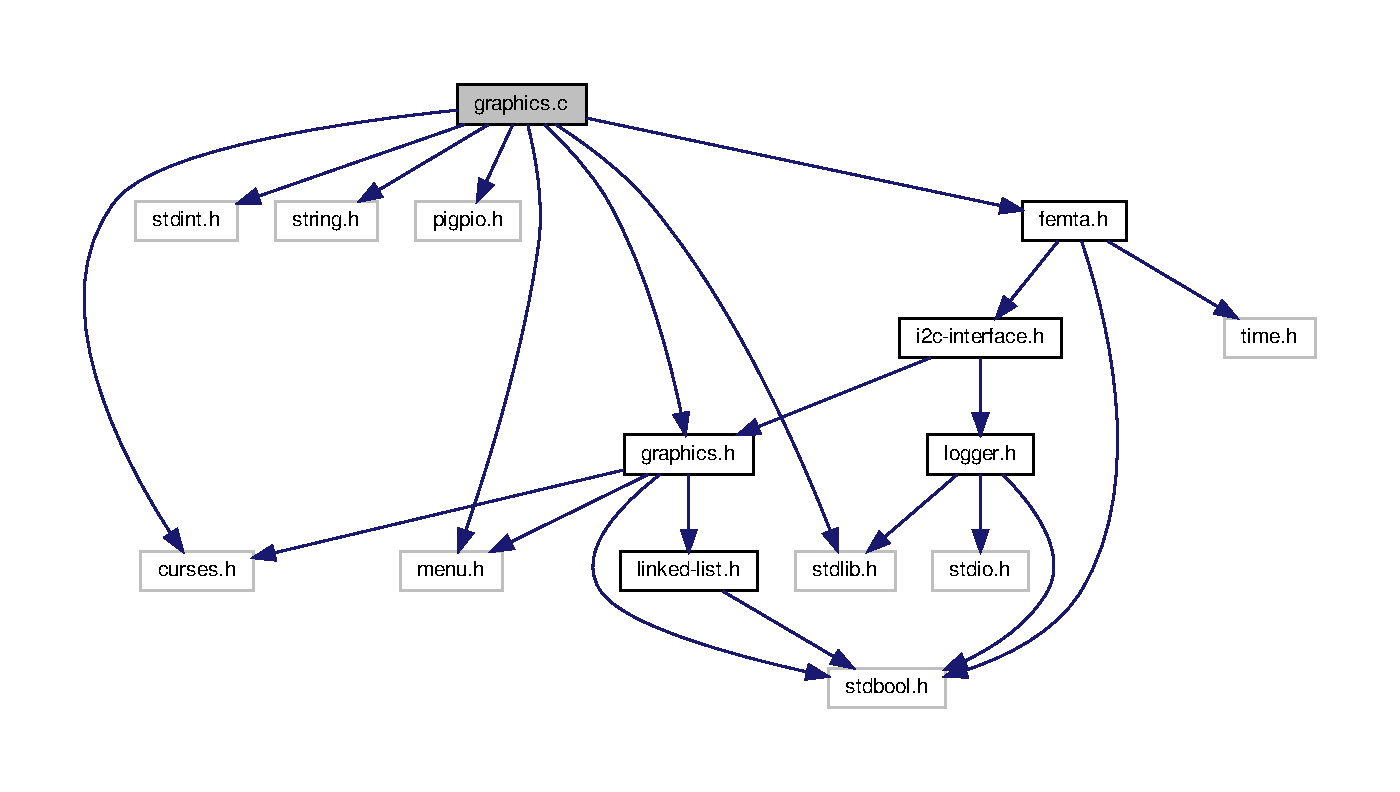
\includegraphics[width=350pt]{graphics_8c__incl}
\end{center}
\end{figure}
\subsection*{Macros}
\begin{DoxyCompactItemize}
\item 
\#define \hyperlink{graphics_8c_a52ede00c016989d352fbe071b104fddf}{N\+U\+M\+B\+E\+R\+\_\+\+O\+F\+\_\+\+M\+O\+D\+U\+L\+ES}~3
\item 
\#define \hyperlink{graphics_8c_ab2d66e2cf934380faec387170c8192fb}{I2\+C\+\_\+\+S\+T\+A\+TE}~2
\item 
\#define \hyperlink{graphics_8c_a30e07560cc19679bdfd1a4a0f375dcce}{U\+A\+R\+T\+\_\+\+S\+T\+A\+TE}~3
\item 
\#define \hyperlink{graphics_8c_a130a4a005f4a37dc0ac6126cc296ee06}{N\+U\+M\+B\+E\+R\+\_\+\+O\+F\+\_\+\+P\+R\+I\+N\+T\+\_\+\+V\+I\+E\+WS}~3
\item 
\#define \hyperlink{graphics_8c_a15c58d8fd08b406512ba49dc85cfec8d}{N\+U\+M\+B\+E\+R\+\_\+\+O\+F\+\_\+\+G\+R\+A\+P\+H\+\_\+\+V\+I\+E\+WS}~1
\item 
\#define \hyperlink{graphics_8c_ab9f720eca0a5b1178cc0432801f8976b}{N\+U\+M\+B\+E\+R\+\_\+\+O\+F\+\_\+\+S\+E\+T\+U\+P\+\_\+\+V\+I\+E\+WS}~1
\end{DoxyCompactItemize}
\subsection*{Functions}
\begin{DoxyCompactItemize}
\item 
void \hyperlink{graphics_8c_a7b38c605caf5bfd616c54fa9a6be4e98}{print\+\_\+window\+\_\+title} ()
\item 
void \hyperlink{graphics_8c_a68b3737c7aa742e27cede272fa1f5901}{initialize\+\_\+graphics} ()
\item 
void \hyperlink{graphics_8c_a801e9e5cdcd5cbc0871a4ff73edc171e}{terminate\+\_\+graphics} ()
\item 
void \hyperlink{graphics_8c_ad65c9b95d3bce65dca68e859e75188ce}{print\+\_\+window\+\_\+title} (W\+I\+N\+D\+OW $\ast$win, int starty, int startx, int width, char $\ast$string, chtype color)
\item 
\hyperlink{structPlot}{Plot} $\ast$ \hyperlink{graphics_8c_a0d74bbdd6f2abaafd1cfb1a12c0e5fe3}{create\+\_\+plot} (char $\ast$name, unsigned char number\+\_\+of\+\_\+lists)
\item 
void \hyperlink{graphics_8c_a22f207fb5603352362eaa769c35a8555}{clear\+\_\+print\+\_\+window} (unsigned char window\+\_\+number)
\item 
void \hyperlink{graphics_8c_af09a3a6eecb74c0b79f9f52e04d9bb05}{print} (unsigned char window\+\_\+number, char $\ast$string, unsigned int color)
\item 
void \hyperlink{graphics_8c_af6f539f61823ed2e8ca170234076ef0a}{erase\+\_\+print\+\_\+window} (unsigned char window\+\_\+number)
\item 
void \hyperlink{graphics_8c_a40fc6b0869e05eb28aceb0faff2a3517}{update\+\_\+state\+\_\+graphic} (unsigned char line, bool state)
\item 
void \hyperlink{graphics_8c_a7556c334f33b2eeb5dad2fbfdafd96ce}{plot\+\_\+add\+\_\+value} (\hyperlink{structPlot}{Plot} $\ast$plot, \hyperlink{structList}{List} $\ast$list, \hyperlink{structNode}{Node} $\ast$node)
\item 
void \hyperlink{graphics_8c_a0149357e966fd1342354a03d37e093c2}{graph\+\_\+plot} (\hyperlink{structPlot}{Plot} $\ast$plot)
\end{DoxyCompactItemize}
\subsection*{Variables}
\begin{DoxyCompactItemize}
\item 
bool \hyperlink{graphics_8c_af633be7c36103ef95413839618e0558b}{ready\+\_\+to\+\_\+graph} = false
\item 
\hyperlink{structprint__view}{print\+\_\+view} $\ast$$\ast$ \hyperlink{graphics_8c_ab988c650efc4bd25b3596d1c880b6231}{print\+\_\+views}
\item 
\hyperlink{structgraph__view}{graph\+\_\+view} $\ast$$\ast$ \hyperlink{graphics_8c_a35a30da8ce1f15d7e2f4bfadde9053f2}{graph\+\_\+views}
\item 
\hyperlink{structsetup__view}{setup\+\_\+view} $\ast$$\ast$ \hyperlink{graphics_8c_a455a28d7f50293e78a3a12f005fa9950}{setup\+\_\+views}
\end{DoxyCompactItemize}


\subsection{Macro Definition Documentation}
\mbox{\Hypertarget{graphics_8c_ab2d66e2cf934380faec387170c8192fb}\label{graphics_8c_ab2d66e2cf934380faec387170c8192fb}} 
\index{graphics.\+c@{graphics.\+c}!I2\+C\+\_\+\+S\+T\+A\+TE@{I2\+C\+\_\+\+S\+T\+A\+TE}}
\index{I2\+C\+\_\+\+S\+T\+A\+TE@{I2\+C\+\_\+\+S\+T\+A\+TE}!graphics.\+c@{graphics.\+c}}
\subsubsection{\texorpdfstring{I2\+C\+\_\+\+S\+T\+A\+TE}{I2C\_STATE}}
{\footnotesize\ttfamily \#define I2\+C\+\_\+\+S\+T\+A\+TE~2}

\mbox{\Hypertarget{graphics_8c_a15c58d8fd08b406512ba49dc85cfec8d}\label{graphics_8c_a15c58d8fd08b406512ba49dc85cfec8d}} 
\index{graphics.\+c@{graphics.\+c}!N\+U\+M\+B\+E\+R\+\_\+\+O\+F\+\_\+\+G\+R\+A\+P\+H\+\_\+\+V\+I\+E\+WS@{N\+U\+M\+B\+E\+R\+\_\+\+O\+F\+\_\+\+G\+R\+A\+P\+H\+\_\+\+V\+I\+E\+WS}}
\index{N\+U\+M\+B\+E\+R\+\_\+\+O\+F\+\_\+\+G\+R\+A\+P\+H\+\_\+\+V\+I\+E\+WS@{N\+U\+M\+B\+E\+R\+\_\+\+O\+F\+\_\+\+G\+R\+A\+P\+H\+\_\+\+V\+I\+E\+WS}!graphics.\+c@{graphics.\+c}}
\subsubsection{\texorpdfstring{N\+U\+M\+B\+E\+R\+\_\+\+O\+F\+\_\+\+G\+R\+A\+P\+H\+\_\+\+V\+I\+E\+WS}{NUMBER\_OF\_GRAPH\_VIEWS}}
{\footnotesize\ttfamily \#define N\+U\+M\+B\+E\+R\+\_\+\+O\+F\+\_\+\+G\+R\+A\+P\+H\+\_\+\+V\+I\+E\+WS~1}

\mbox{\Hypertarget{graphics_8c_a52ede00c016989d352fbe071b104fddf}\label{graphics_8c_a52ede00c016989d352fbe071b104fddf}} 
\index{graphics.\+c@{graphics.\+c}!N\+U\+M\+B\+E\+R\+\_\+\+O\+F\+\_\+\+M\+O\+D\+U\+L\+ES@{N\+U\+M\+B\+E\+R\+\_\+\+O\+F\+\_\+\+M\+O\+D\+U\+L\+ES}}
\index{N\+U\+M\+B\+E\+R\+\_\+\+O\+F\+\_\+\+M\+O\+D\+U\+L\+ES@{N\+U\+M\+B\+E\+R\+\_\+\+O\+F\+\_\+\+M\+O\+D\+U\+L\+ES}!graphics.\+c@{graphics.\+c}}
\subsubsection{\texorpdfstring{N\+U\+M\+B\+E\+R\+\_\+\+O\+F\+\_\+\+M\+O\+D\+U\+L\+ES}{NUMBER\_OF\_MODULES}}
{\footnotesize\ttfamily \#define N\+U\+M\+B\+E\+R\+\_\+\+O\+F\+\_\+\+M\+O\+D\+U\+L\+ES~3}

\mbox{\Hypertarget{graphics_8c_a130a4a005f4a37dc0ac6126cc296ee06}\label{graphics_8c_a130a4a005f4a37dc0ac6126cc296ee06}} 
\index{graphics.\+c@{graphics.\+c}!N\+U\+M\+B\+E\+R\+\_\+\+O\+F\+\_\+\+P\+R\+I\+N\+T\+\_\+\+V\+I\+E\+WS@{N\+U\+M\+B\+E\+R\+\_\+\+O\+F\+\_\+\+P\+R\+I\+N\+T\+\_\+\+V\+I\+E\+WS}}
\index{N\+U\+M\+B\+E\+R\+\_\+\+O\+F\+\_\+\+P\+R\+I\+N\+T\+\_\+\+V\+I\+E\+WS@{N\+U\+M\+B\+E\+R\+\_\+\+O\+F\+\_\+\+P\+R\+I\+N\+T\+\_\+\+V\+I\+E\+WS}!graphics.\+c@{graphics.\+c}}
\subsubsection{\texorpdfstring{N\+U\+M\+B\+E\+R\+\_\+\+O\+F\+\_\+\+P\+R\+I\+N\+T\+\_\+\+V\+I\+E\+WS}{NUMBER\_OF\_PRINT\_VIEWS}}
{\footnotesize\ttfamily \#define N\+U\+M\+B\+E\+R\+\_\+\+O\+F\+\_\+\+P\+R\+I\+N\+T\+\_\+\+V\+I\+E\+WS~3}

\mbox{\Hypertarget{graphics_8c_ab9f720eca0a5b1178cc0432801f8976b}\label{graphics_8c_ab9f720eca0a5b1178cc0432801f8976b}} 
\index{graphics.\+c@{graphics.\+c}!N\+U\+M\+B\+E\+R\+\_\+\+O\+F\+\_\+\+S\+E\+T\+U\+P\+\_\+\+V\+I\+E\+WS@{N\+U\+M\+B\+E\+R\+\_\+\+O\+F\+\_\+\+S\+E\+T\+U\+P\+\_\+\+V\+I\+E\+WS}}
\index{N\+U\+M\+B\+E\+R\+\_\+\+O\+F\+\_\+\+S\+E\+T\+U\+P\+\_\+\+V\+I\+E\+WS@{N\+U\+M\+B\+E\+R\+\_\+\+O\+F\+\_\+\+S\+E\+T\+U\+P\+\_\+\+V\+I\+E\+WS}!graphics.\+c@{graphics.\+c}}
\subsubsection{\texorpdfstring{N\+U\+M\+B\+E\+R\+\_\+\+O\+F\+\_\+\+S\+E\+T\+U\+P\+\_\+\+V\+I\+E\+WS}{NUMBER\_OF\_SETUP\_VIEWS}}
{\footnotesize\ttfamily \#define N\+U\+M\+B\+E\+R\+\_\+\+O\+F\+\_\+\+S\+E\+T\+U\+P\+\_\+\+V\+I\+E\+WS~1}

\mbox{\Hypertarget{graphics_8c_a30e07560cc19679bdfd1a4a0f375dcce}\label{graphics_8c_a30e07560cc19679bdfd1a4a0f375dcce}} 
\index{graphics.\+c@{graphics.\+c}!U\+A\+R\+T\+\_\+\+S\+T\+A\+TE@{U\+A\+R\+T\+\_\+\+S\+T\+A\+TE}}
\index{U\+A\+R\+T\+\_\+\+S\+T\+A\+TE@{U\+A\+R\+T\+\_\+\+S\+T\+A\+TE}!graphics.\+c@{graphics.\+c}}
\subsubsection{\texorpdfstring{U\+A\+R\+T\+\_\+\+S\+T\+A\+TE}{UART\_STATE}}
{\footnotesize\ttfamily \#define U\+A\+R\+T\+\_\+\+S\+T\+A\+TE~3}



\subsection{Function Documentation}
\mbox{\Hypertarget{graphics_8c_a22f207fb5603352362eaa769c35a8555}\label{graphics_8c_a22f207fb5603352362eaa769c35a8555}} 
\index{graphics.\+c@{graphics.\+c}!clear\+\_\+print\+\_\+window@{clear\+\_\+print\+\_\+window}}
\index{clear\+\_\+print\+\_\+window@{clear\+\_\+print\+\_\+window}!graphics.\+c@{graphics.\+c}}
\subsubsection{\texorpdfstring{clear\+\_\+print\+\_\+window()}{clear\_print\_window()}}
{\footnotesize\ttfamily void clear\+\_\+print\+\_\+window (\begin{DoxyParamCaption}\item[{unsigned char}]{window\+\_\+number }\end{DoxyParamCaption})}

Here is the caller graph for this function\+:
\nopagebreak
\begin{figure}[H]
\begin{center}
\leavevmode
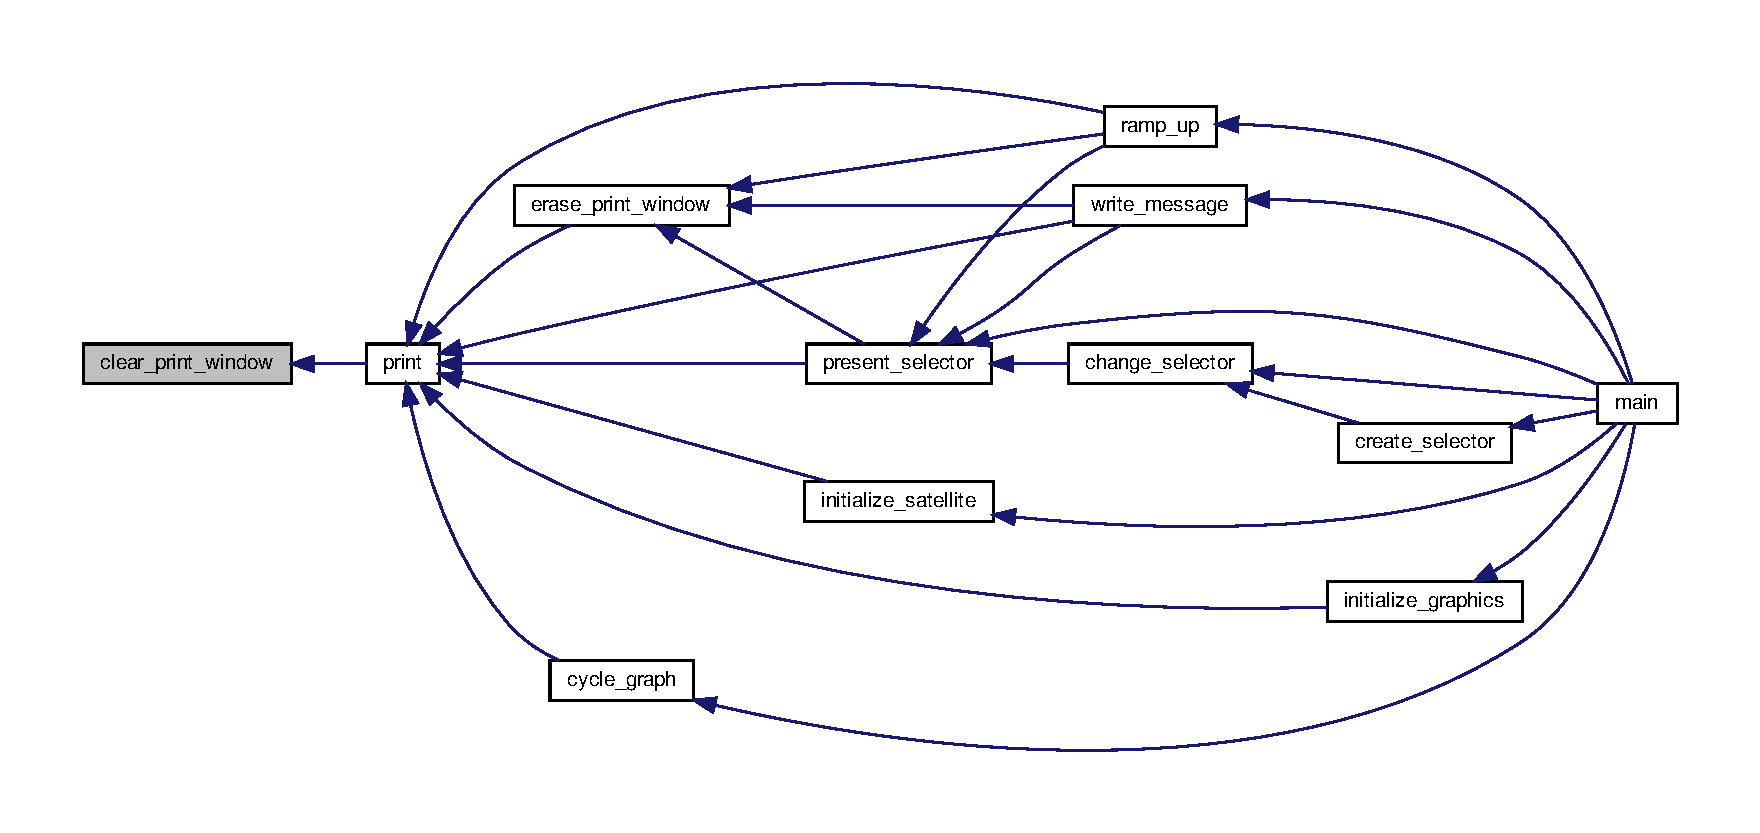
\includegraphics[width=350pt]{graphics_8c_a22f207fb5603352362eaa769c35a8555_icgraph}
\end{center}
\end{figure}
\mbox{\Hypertarget{graphics_8c_a0d74bbdd6f2abaafd1cfb1a12c0e5fe3}\label{graphics_8c_a0d74bbdd6f2abaafd1cfb1a12c0e5fe3}} 
\index{graphics.\+c@{graphics.\+c}!create\+\_\+plot@{create\+\_\+plot}}
\index{create\+\_\+plot@{create\+\_\+plot}!graphics.\+c@{graphics.\+c}}
\subsubsection{\texorpdfstring{create\+\_\+plot()}{create\_plot()}}
{\footnotesize\ttfamily \hyperlink{structPlot}{Plot}$\ast$ create\+\_\+plot (\begin{DoxyParamCaption}\item[{char $\ast$}]{name,  }\item[{unsigned char}]{number\+\_\+of\+\_\+lists }\end{DoxyParamCaption})}

Here is the call graph for this function\+:
\nopagebreak
\begin{figure}[H]
\begin{center}
\leavevmode
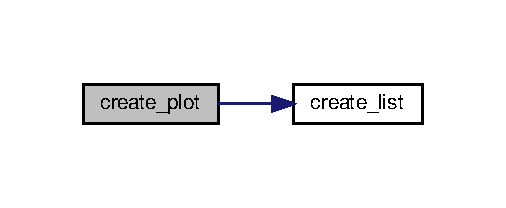
\includegraphics[width=243pt]{graphics_8c_a0d74bbdd6f2abaafd1cfb1a12c0e5fe3_cgraph}
\end{center}
\end{figure}
Here is the caller graph for this function\+:
\nopagebreak
\begin{figure}[H]
\begin{center}
\leavevmode
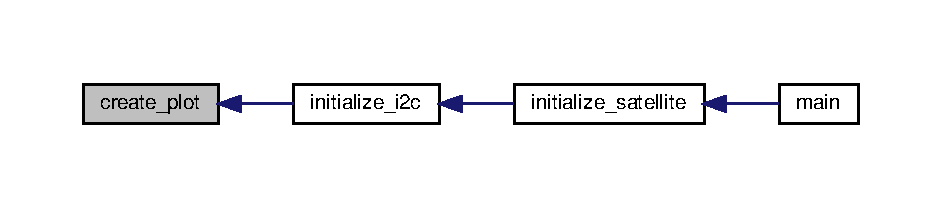
\includegraphics[width=350pt]{graphics_8c_a0d74bbdd6f2abaafd1cfb1a12c0e5fe3_icgraph}
\end{center}
\end{figure}
\mbox{\Hypertarget{graphics_8c_af6f539f61823ed2e8ca170234076ef0a}\label{graphics_8c_af6f539f61823ed2e8ca170234076ef0a}} 
\index{graphics.\+c@{graphics.\+c}!erase\+\_\+print\+\_\+window@{erase\+\_\+print\+\_\+window}}
\index{erase\+\_\+print\+\_\+window@{erase\+\_\+print\+\_\+window}!graphics.\+c@{graphics.\+c}}
\subsubsection{\texorpdfstring{erase\+\_\+print\+\_\+window()}{erase\_print\_window()}}
{\footnotesize\ttfamily void erase\+\_\+print\+\_\+window (\begin{DoxyParamCaption}\item[{unsigned char}]{window\+\_\+number }\end{DoxyParamCaption})}

Here is the call graph for this function\+:
\nopagebreak
\begin{figure}[H]
\begin{center}
\leavevmode
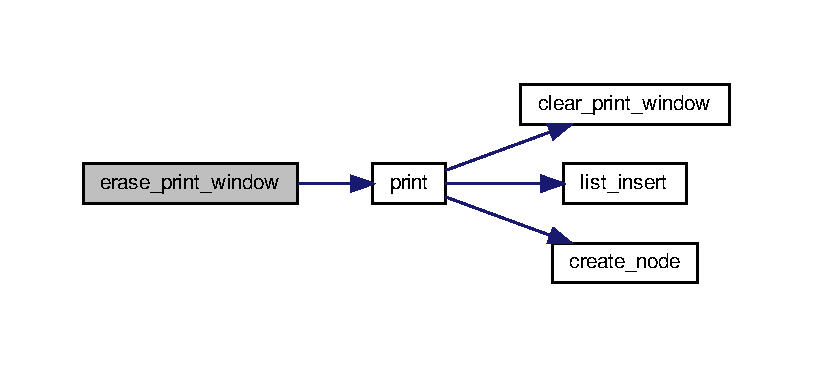
\includegraphics[width=350pt]{graphics_8c_af6f539f61823ed2e8ca170234076ef0a_cgraph}
\end{center}
\end{figure}
Here is the caller graph for this function\+:
\nopagebreak
\begin{figure}[H]
\begin{center}
\leavevmode
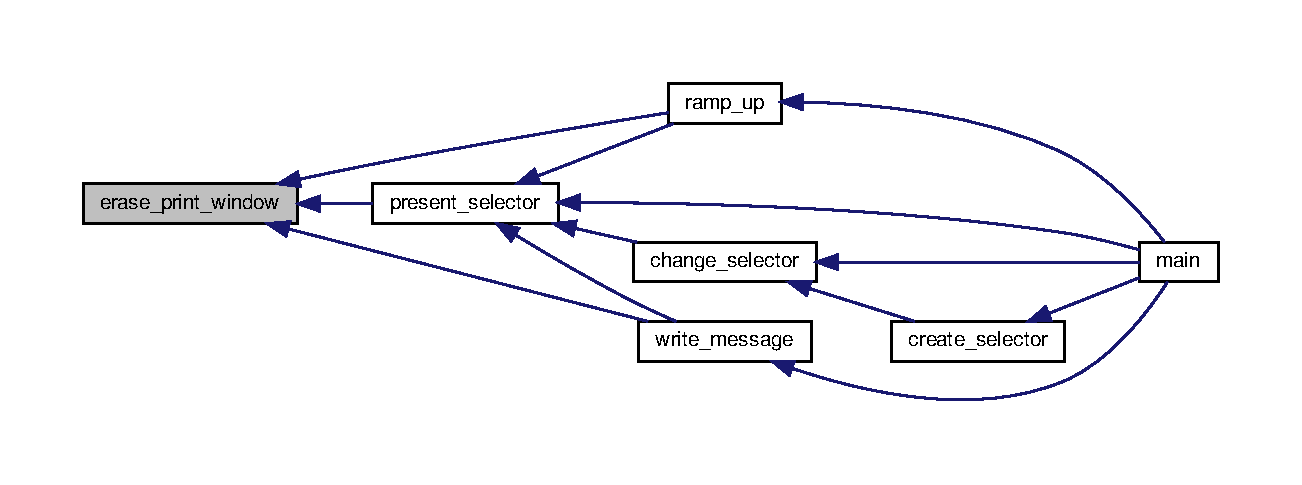
\includegraphics[width=350pt]{graphics_8c_af6f539f61823ed2e8ca170234076ef0a_icgraph}
\end{center}
\end{figure}
\mbox{\Hypertarget{graphics_8c_a0149357e966fd1342354a03d37e093c2}\label{graphics_8c_a0149357e966fd1342354a03d37e093c2}} 
\index{graphics.\+c@{graphics.\+c}!graph\+\_\+plot@{graph\+\_\+plot}}
\index{graph\+\_\+plot@{graph\+\_\+plot}!graphics.\+c@{graphics.\+c}}
\subsubsection{\texorpdfstring{graph\+\_\+plot()}{graph\_plot()}}
{\footnotesize\ttfamily void graph\+\_\+plot (\begin{DoxyParamCaption}\item[{\hyperlink{structPlot}{Plot} $\ast$}]{plot }\end{DoxyParamCaption})}

Here is the call graph for this function\+:
\nopagebreak
\begin{figure}[H]
\begin{center}
\leavevmode
\includegraphics[width=273pt]{graphics_8c_a0149357e966fd1342354a03d37e093c2_cgraph}
\end{center}
\end{figure}
Here is the caller graph for this function\+:
\nopagebreak
\begin{figure}[H]
\begin{center}
\leavevmode
\includegraphics[width=350pt]{graphics_8c_a0149357e966fd1342354a03d37e093c2_icgraph}
\end{center}
\end{figure}
\mbox{\Hypertarget{graphics_8c_a68b3737c7aa742e27cede272fa1f5901}\label{graphics_8c_a68b3737c7aa742e27cede272fa1f5901}} 
\index{graphics.\+c@{graphics.\+c}!initialize\+\_\+graphics@{initialize\+\_\+graphics}}
\index{initialize\+\_\+graphics@{initialize\+\_\+graphics}!graphics.\+c@{graphics.\+c}}
\subsubsection{\texorpdfstring{initialize\+\_\+graphics()}{initialize\_graphics()}}
{\footnotesize\ttfamily void initialize\+\_\+graphics (\begin{DoxyParamCaption}{ }\end{DoxyParamCaption})}

Here is the call graph for this function\+:
\nopagebreak
\begin{figure}[H]
\begin{center}
\leavevmode
\includegraphics[width=350pt]{graphics_8c_a68b3737c7aa742e27cede272fa1f5901_cgraph}
\end{center}
\end{figure}
Here is the caller graph for this function\+:
\nopagebreak
\begin{figure}[H]
\begin{center}
\leavevmode
\includegraphics[width=248pt]{graphics_8c_a68b3737c7aa742e27cede272fa1f5901_icgraph}
\end{center}
\end{figure}
\mbox{\Hypertarget{graphics_8c_a7556c334f33b2eeb5dad2fbfdafd96ce}\label{graphics_8c_a7556c334f33b2eeb5dad2fbfdafd96ce}} 
\index{graphics.\+c@{graphics.\+c}!plot\+\_\+add\+\_\+value@{plot\+\_\+add\+\_\+value}}
\index{plot\+\_\+add\+\_\+value@{plot\+\_\+add\+\_\+value}!graphics.\+c@{graphics.\+c}}
\subsubsection{\texorpdfstring{plot\+\_\+add\+\_\+value()}{plot\_add\_value()}}
{\footnotesize\ttfamily void plot\+\_\+add\+\_\+value (\begin{DoxyParamCaption}\item[{\hyperlink{structPlot}{Plot} $\ast$}]{plot,  }\item[{\hyperlink{structList}{List} $\ast$}]{list,  }\item[{\hyperlink{structNode}{Node} $\ast$}]{node }\end{DoxyParamCaption})}

Here is the call graph for this function\+:
\nopagebreak
\begin{figure}[H]
\begin{center}
\leavevmode
\includegraphics[width=257pt]{graphics_8c_a7556c334f33b2eeb5dad2fbfdafd96ce_cgraph}
\end{center}
\end{figure}
Here is the caller graph for this function\+:
\nopagebreak
\begin{figure}[H]
\begin{center}
\leavevmode
\includegraphics[width=350pt]{graphics_8c_a7556c334f33b2eeb5dad2fbfdafd96ce_icgraph}
\end{center}
\end{figure}
\mbox{\Hypertarget{graphics_8c_af09a3a6eecb74c0b79f9f52e04d9bb05}\label{graphics_8c_af09a3a6eecb74c0b79f9f52e04d9bb05}} 
\index{graphics.\+c@{graphics.\+c}!print@{print}}
\index{print@{print}!graphics.\+c@{graphics.\+c}}
\subsubsection{\texorpdfstring{print()}{print()}}
{\footnotesize\ttfamily void print (\begin{DoxyParamCaption}\item[{unsigned char}]{window\+\_\+number,  }\item[{char $\ast$}]{string,  }\item[{unsigned int}]{color }\end{DoxyParamCaption})}

Here is the call graph for this function\+:
\nopagebreak
\begin{figure}[H]
\begin{center}
\leavevmode
\includegraphics[width=251pt]{graphics_8c_af09a3a6eecb74c0b79f9f52e04d9bb05_cgraph}
\end{center}
\end{figure}
Here is the caller graph for this function\+:
\nopagebreak
\begin{figure}[H]
\begin{center}
\leavevmode
\includegraphics[width=350pt]{graphics_8c_af09a3a6eecb74c0b79f9f52e04d9bb05_icgraph}
\end{center}
\end{figure}
\mbox{\Hypertarget{graphics_8c_a7b38c605caf5bfd616c54fa9a6be4e98}\label{graphics_8c_a7b38c605caf5bfd616c54fa9a6be4e98}} 
\index{graphics.\+c@{graphics.\+c}!print\+\_\+window\+\_\+title@{print\+\_\+window\+\_\+title}}
\index{print\+\_\+window\+\_\+title@{print\+\_\+window\+\_\+title}!graphics.\+c@{graphics.\+c}}
\subsubsection{\texorpdfstring{print\+\_\+window\+\_\+title()}{print\_window\_title()}\hspace{0.1cm}{\footnotesize\ttfamily [1/2]}}
{\footnotesize\ttfamily void print\+\_\+window\+\_\+title (\begin{DoxyParamCaption}{ }\end{DoxyParamCaption})}

Here is the caller graph for this function\+:
\nopagebreak
\begin{figure}[H]
\begin{center}
\leavevmode
\includegraphics[width=350pt]{graphics_8c_a7b38c605caf5bfd616c54fa9a6be4e98_icgraph}
\end{center}
\end{figure}
\mbox{\Hypertarget{graphics_8c_ad65c9b95d3bce65dca68e859e75188ce}\label{graphics_8c_ad65c9b95d3bce65dca68e859e75188ce}} 
\index{graphics.\+c@{graphics.\+c}!print\+\_\+window\+\_\+title@{print\+\_\+window\+\_\+title}}
\index{print\+\_\+window\+\_\+title@{print\+\_\+window\+\_\+title}!graphics.\+c@{graphics.\+c}}
\subsubsection{\texorpdfstring{print\+\_\+window\+\_\+title()}{print\_window\_title()}\hspace{0.1cm}{\footnotesize\ttfamily [2/2]}}
{\footnotesize\ttfamily void print\+\_\+window\+\_\+title (\begin{DoxyParamCaption}\item[{W\+I\+N\+D\+OW $\ast$}]{win,  }\item[{int}]{starty,  }\item[{int}]{startx,  }\item[{int}]{width,  }\item[{char $\ast$}]{string,  }\item[{chtype}]{color }\end{DoxyParamCaption})}

\mbox{\Hypertarget{graphics_8c_a801e9e5cdcd5cbc0871a4ff73edc171e}\label{graphics_8c_a801e9e5cdcd5cbc0871a4ff73edc171e}} 
\index{graphics.\+c@{graphics.\+c}!terminate\+\_\+graphics@{terminate\+\_\+graphics}}
\index{terminate\+\_\+graphics@{terminate\+\_\+graphics}!graphics.\+c@{graphics.\+c}}
\subsubsection{\texorpdfstring{terminate\+\_\+graphics()}{terminate\_graphics()}}
{\footnotesize\ttfamily void terminate\+\_\+graphics (\begin{DoxyParamCaption}{ }\end{DoxyParamCaption})}

Here is the caller graph for this function\+:
\nopagebreak
\begin{figure}[H]
\begin{center}
\leavevmode
\includegraphics[width=253pt]{graphics_8c_a801e9e5cdcd5cbc0871a4ff73edc171e_icgraph}
\end{center}
\end{figure}
\mbox{\Hypertarget{graphics_8c_a40fc6b0869e05eb28aceb0faff2a3517}\label{graphics_8c_a40fc6b0869e05eb28aceb0faff2a3517}} 
\index{graphics.\+c@{graphics.\+c}!update\+\_\+state\+\_\+graphic@{update\+\_\+state\+\_\+graphic}}
\index{update\+\_\+state\+\_\+graphic@{update\+\_\+state\+\_\+graphic}!graphics.\+c@{graphics.\+c}}
\subsubsection{\texorpdfstring{update\+\_\+state\+\_\+graphic()}{update\_state\_graphic()}}
{\footnotesize\ttfamily void update\+\_\+state\+\_\+graphic (\begin{DoxyParamCaption}\item[{unsigned char}]{line,  }\item[{bool}]{state }\end{DoxyParamCaption})}



\subsection{Variable Documentation}
\mbox{\Hypertarget{graphics_8c_a35a30da8ce1f15d7e2f4bfadde9053f2}\label{graphics_8c_a35a30da8ce1f15d7e2f4bfadde9053f2}} 
\index{graphics.\+c@{graphics.\+c}!graph\+\_\+views@{graph\+\_\+views}}
\index{graph\+\_\+views@{graph\+\_\+views}!graphics.\+c@{graphics.\+c}}
\subsubsection{\texorpdfstring{graph\+\_\+views}{graph\_views}}
{\footnotesize\ttfamily \hyperlink{structgraph__view}{graph\+\_\+view}$\ast$$\ast$ graph\+\_\+views}

\mbox{\Hypertarget{graphics_8c_ab988c650efc4bd25b3596d1c880b6231}\label{graphics_8c_ab988c650efc4bd25b3596d1c880b6231}} 
\index{graphics.\+c@{graphics.\+c}!print\+\_\+views@{print\+\_\+views}}
\index{print\+\_\+views@{print\+\_\+views}!graphics.\+c@{graphics.\+c}}
\subsubsection{\texorpdfstring{print\+\_\+views}{print\_views}}
{\footnotesize\ttfamily \hyperlink{structprint__view}{print\+\_\+view}$\ast$$\ast$ print\+\_\+views}

\mbox{\Hypertarget{graphics_8c_af633be7c36103ef95413839618e0558b}\label{graphics_8c_af633be7c36103ef95413839618e0558b}} 
\index{graphics.\+c@{graphics.\+c}!ready\+\_\+to\+\_\+graph@{ready\+\_\+to\+\_\+graph}}
\index{ready\+\_\+to\+\_\+graph@{ready\+\_\+to\+\_\+graph}!graphics.\+c@{graphics.\+c}}
\subsubsection{\texorpdfstring{ready\+\_\+to\+\_\+graph}{ready\_to\_graph}}
{\footnotesize\ttfamily bool ready\+\_\+to\+\_\+graph = false}

\mbox{\Hypertarget{graphics_8c_a455a28d7f50293e78a3a12f005fa9950}\label{graphics_8c_a455a28d7f50293e78a3a12f005fa9950}} 
\index{graphics.\+c@{graphics.\+c}!setup\+\_\+views@{setup\+\_\+views}}
\index{setup\+\_\+views@{setup\+\_\+views}!graphics.\+c@{graphics.\+c}}
\subsubsection{\texorpdfstring{setup\+\_\+views}{setup\_views}}
{\footnotesize\ttfamily \hyperlink{structsetup__view}{setup\+\_\+view}$\ast$$\ast$ setup\+\_\+views}


\hypertarget{graphics_8h}{}\section{graphics.\+h File Reference}
\label{graphics_8h}\index{graphics.\+h@{graphics.\+h}}
{\ttfamily \#include $<$stdbool.\+h$>$}\newline
{\ttfamily \#include $<$curses.\+h$>$}\newline
{\ttfamily \#include $<$menu.\+h$>$}\newline
{\ttfamily \#include \char`\"{}linked-\/list.\+h\char`\"{}}\newline
Include dependency graph for graphics.\+h\+:\nopagebreak
\begin{figure}[H]
\begin{center}
\leavevmode
\includegraphics[width=298pt]{graphics_8h__incl}
\end{center}
\end{figure}
This graph shows which files directly or indirectly include this file\+:
\nopagebreak
\begin{figure}[H]
\begin{center}
\leavevmode
\includegraphics[width=350pt]{graphics_8h__dep__incl}
\end{center}
\end{figure}
\subsection*{Classes}
\begin{DoxyCompactItemize}
\item 
struct \hyperlink{structView}{View}
\item 
struct \hyperlink{structPlot}{Plot}
\item 
struct \hyperlink{structprint__view}{print\+\_\+view}
\item 
struct \hyperlink{structgraph__view}{graph\+\_\+view}
\item 
struct \hyperlink{structsetup__view}{setup\+\_\+view}
\end{DoxyCompactItemize}
\subsection*{Macros}
\begin{DoxyCompactItemize}
\item 
\#define \hyperlink{graphics_8h_a6df7958d438966bf34dc9524cbf7d8f0}{G\+E\+N\+E\+R\+A\+L\+\_\+\+W\+I\+N\+D\+OW}~0
\item 
\#define \hyperlink{graphics_8h_a3f4bf8af94b8c1c45ee5c16d05c235c1}{C\+O\+N\+T\+R\+O\+L\+\_\+\+W\+I\+N\+D\+OW}~1
\item 
\#define \hyperlink{graphics_8h_afea4087ad18bef55383c783669b5f3c6}{O\+P\+E\+R\+A\+T\+E\+\_\+\+W\+I\+N\+D\+OW}~2
\end{DoxyCompactItemize}
\subsection*{Typedefs}
\begin{DoxyCompactItemize}
\item 
typedef struct \hyperlink{structView}{View} \hyperlink{graphics_8h_a4db1f4ea505b597e255278b110002b63}{View}
\item 
typedef struct \hyperlink{structPlot}{Plot} \hyperlink{graphics_8h_a1c9783a619ececaff6ca8cd670a2f998}{Plot}
\item 
typedef struct \hyperlink{structprint__view}{print\+\_\+view} \hyperlink{graphics_8h_a8adb006ef95ecf838877a80bd9fcc052}{print\+\_\+view}
\item 
typedef struct \hyperlink{structgraph__view}{graph\+\_\+view} \hyperlink{graphics_8h_ab4cafed81f535c2bcaa088caa1c9f914}{graph\+\_\+view}
\item 
typedef struct \hyperlink{structsetup__view}{setup\+\_\+view} \hyperlink{graphics_8h_ae3c6a8958ebd350426acf84ed95411b9}{setup\+\_\+view}
\end{DoxyCompactItemize}
\subsection*{Functions}
\begin{DoxyCompactItemize}
\item 
void \hyperlink{graphics_8h_a68b3737c7aa742e27cede272fa1f5901}{initialize\+\_\+graphics} ()
\item 
void \hyperlink{graphics_8h_a801e9e5cdcd5cbc0871a4ff73edc171e}{terminate\+\_\+graphics} ()
\item 
void \hyperlink{graphics_8h_af09a3a6eecb74c0b79f9f52e04d9bb05}{print} (unsigned char window\+\_\+number, char $\ast$string, unsigned int color)
\item 
void \hyperlink{graphics_8h_a22f207fb5603352362eaa769c35a8555}{clear\+\_\+print\+\_\+window} (unsigned char window\+\_\+number)
\item 
void \hyperlink{graphics_8h_af6f539f61823ed2e8ca170234076ef0a}{erase\+\_\+print\+\_\+window} (unsigned char window\+\_\+number)
\item 
void \hyperlink{graphics_8h_a40fc6b0869e05eb28aceb0faff2a3517}{update\+\_\+state\+\_\+graphic} (unsigned char line, bool state)
\item 
void \hyperlink{graphics_8h_a0149357e966fd1342354a03d37e093c2}{graph\+\_\+plot} (\hyperlink{structPlot}{Plot} $\ast$plot)
\item 
void \hyperlink{graphics_8h_a7556c334f33b2eeb5dad2fbfdafd96ce}{plot\+\_\+add\+\_\+value} (\hyperlink{structPlot}{Plot} $\ast$plot, \hyperlink{structList}{List} $\ast$list, \hyperlink{structNode}{Node} $\ast$node)
\item 
\hyperlink{structPlot}{Plot} $\ast$ \hyperlink{graphics_8h_a0d74bbdd6f2abaafd1cfb1a12c0e5fe3}{create\+\_\+plot} (char $\ast$name, unsigned char number\+\_\+of\+\_\+lists)
\end{DoxyCompactItemize}
\subsection*{Variables}
\begin{DoxyCompactItemize}
\item 
\hyperlink{structprint__view}{print\+\_\+view} $\ast$$\ast$ \hyperlink{graphics_8h_ab988c650efc4bd25b3596d1c880b6231}{print\+\_\+views}
\item 
\hyperlink{structgraph__view}{graph\+\_\+view} $\ast$$\ast$ \hyperlink{graphics_8h_a35a30da8ce1f15d7e2f4bfadde9053f2}{graph\+\_\+views}
\item 
\hyperlink{structsetup__view}{setup\+\_\+view} $\ast$$\ast$ \hyperlink{graphics_8h_a455a28d7f50293e78a3a12f005fa9950}{setup\+\_\+views}
\item 
unsigned char \hyperlink{graphics_8h_a49d2b92059a29312ac2727b0ed2b8bc4}{number\+\_\+of\+\_\+data\+\_\+points\+\_\+plottable}
\item 
\hyperlink{structPlot}{Plot} $\ast$ \hyperlink{graphics_8h_a313e20a66c8833e422e3f0180bce3757}{graph\+\_\+owner}
\item 
\hyperlink{structPlot}{Plot} $\ast$$\ast$ \hyperlink{graphics_8h_ad9c8da25c90166f9515c8f19f7f409dc}{all\+\_\+possible\+\_\+owners}
\item 
\hyperlink{structList}{List} $\ast$ \hyperlink{graphics_8h_afc01ec0b1c938ce19a65f94f81f6746c}{owner\+\_\+index\+\_\+list}
\item 
\hyperlink{structNode}{Node} $\ast$ \hyperlink{graphics_8h_a0256791883a8ea626376399c88f02040}{graph\+\_\+owner\+\_\+index\+\_\+node}
\end{DoxyCompactItemize}


\subsection{Macro Definition Documentation}
\mbox{\Hypertarget{graphics_8h_a3f4bf8af94b8c1c45ee5c16d05c235c1}\label{graphics_8h_a3f4bf8af94b8c1c45ee5c16d05c235c1}} 
\index{graphics.\+h@{graphics.\+h}!C\+O\+N\+T\+R\+O\+L\+\_\+\+W\+I\+N\+D\+OW@{C\+O\+N\+T\+R\+O\+L\+\_\+\+W\+I\+N\+D\+OW}}
\index{C\+O\+N\+T\+R\+O\+L\+\_\+\+W\+I\+N\+D\+OW@{C\+O\+N\+T\+R\+O\+L\+\_\+\+W\+I\+N\+D\+OW}!graphics.\+h@{graphics.\+h}}
\subsubsection{\texorpdfstring{C\+O\+N\+T\+R\+O\+L\+\_\+\+W\+I\+N\+D\+OW}{CONTROL\_WINDOW}}
{\footnotesize\ttfamily \#define C\+O\+N\+T\+R\+O\+L\+\_\+\+W\+I\+N\+D\+OW~1}

\mbox{\Hypertarget{graphics_8h_a6df7958d438966bf34dc9524cbf7d8f0}\label{graphics_8h_a6df7958d438966bf34dc9524cbf7d8f0}} 
\index{graphics.\+h@{graphics.\+h}!G\+E\+N\+E\+R\+A\+L\+\_\+\+W\+I\+N\+D\+OW@{G\+E\+N\+E\+R\+A\+L\+\_\+\+W\+I\+N\+D\+OW}}
\index{G\+E\+N\+E\+R\+A\+L\+\_\+\+W\+I\+N\+D\+OW@{G\+E\+N\+E\+R\+A\+L\+\_\+\+W\+I\+N\+D\+OW}!graphics.\+h@{graphics.\+h}}
\subsubsection{\texorpdfstring{G\+E\+N\+E\+R\+A\+L\+\_\+\+W\+I\+N\+D\+OW}{GENERAL\_WINDOW}}
{\footnotesize\ttfamily \#define G\+E\+N\+E\+R\+A\+L\+\_\+\+W\+I\+N\+D\+OW~0}

\mbox{\Hypertarget{graphics_8h_afea4087ad18bef55383c783669b5f3c6}\label{graphics_8h_afea4087ad18bef55383c783669b5f3c6}} 
\index{graphics.\+h@{graphics.\+h}!O\+P\+E\+R\+A\+T\+E\+\_\+\+W\+I\+N\+D\+OW@{O\+P\+E\+R\+A\+T\+E\+\_\+\+W\+I\+N\+D\+OW}}
\index{O\+P\+E\+R\+A\+T\+E\+\_\+\+W\+I\+N\+D\+OW@{O\+P\+E\+R\+A\+T\+E\+\_\+\+W\+I\+N\+D\+OW}!graphics.\+h@{graphics.\+h}}
\subsubsection{\texorpdfstring{O\+P\+E\+R\+A\+T\+E\+\_\+\+W\+I\+N\+D\+OW}{OPERATE\_WINDOW}}
{\footnotesize\ttfamily \#define O\+P\+E\+R\+A\+T\+E\+\_\+\+W\+I\+N\+D\+OW~2}



\subsection{Typedef Documentation}
\mbox{\Hypertarget{graphics_8h_ab4cafed81f535c2bcaa088caa1c9f914}\label{graphics_8h_ab4cafed81f535c2bcaa088caa1c9f914}} 
\index{graphics.\+h@{graphics.\+h}!graph\+\_\+view@{graph\+\_\+view}}
\index{graph\+\_\+view@{graph\+\_\+view}!graphics.\+h@{graphics.\+h}}
\subsubsection{\texorpdfstring{graph\+\_\+view}{graph\_view}}
{\footnotesize\ttfamily typedef struct \hyperlink{structgraph__view}{graph\+\_\+view}  \hyperlink{structgraph__view}{graph\+\_\+view}}

\mbox{\Hypertarget{graphics_8h_a1c9783a619ececaff6ca8cd670a2f998}\label{graphics_8h_a1c9783a619ececaff6ca8cd670a2f998}} 
\index{graphics.\+h@{graphics.\+h}!Plot@{Plot}}
\index{Plot@{Plot}!graphics.\+h@{graphics.\+h}}
\subsubsection{\texorpdfstring{Plot}{Plot}}
{\footnotesize\ttfamily typedef struct \hyperlink{structPlot}{Plot}  \hyperlink{structPlot}{Plot}}

\mbox{\Hypertarget{graphics_8h_a8adb006ef95ecf838877a80bd9fcc052}\label{graphics_8h_a8adb006ef95ecf838877a80bd9fcc052}} 
\index{graphics.\+h@{graphics.\+h}!print\+\_\+view@{print\+\_\+view}}
\index{print\+\_\+view@{print\+\_\+view}!graphics.\+h@{graphics.\+h}}
\subsubsection{\texorpdfstring{print\+\_\+view}{print\_view}}
{\footnotesize\ttfamily typedef struct \hyperlink{structprint__view}{print\+\_\+view}  \hyperlink{structprint__view}{print\+\_\+view}}

\mbox{\Hypertarget{graphics_8h_ae3c6a8958ebd350426acf84ed95411b9}\label{graphics_8h_ae3c6a8958ebd350426acf84ed95411b9}} 
\index{graphics.\+h@{graphics.\+h}!setup\+\_\+view@{setup\+\_\+view}}
\index{setup\+\_\+view@{setup\+\_\+view}!graphics.\+h@{graphics.\+h}}
\subsubsection{\texorpdfstring{setup\+\_\+view}{setup\_view}}
{\footnotesize\ttfamily typedef struct \hyperlink{structsetup__view}{setup\+\_\+view}  \hyperlink{structsetup__view}{setup\+\_\+view}}

\mbox{\Hypertarget{graphics_8h_a4db1f4ea505b597e255278b110002b63}\label{graphics_8h_a4db1f4ea505b597e255278b110002b63}} 
\index{graphics.\+h@{graphics.\+h}!View@{View}}
\index{View@{View}!graphics.\+h@{graphics.\+h}}
\subsubsection{\texorpdfstring{View}{View}}
{\footnotesize\ttfamily typedef struct \hyperlink{structView}{View}  \hyperlink{structView}{View}}



\subsection{Function Documentation}
\mbox{\Hypertarget{graphics_8h_a22f207fb5603352362eaa769c35a8555}\label{graphics_8h_a22f207fb5603352362eaa769c35a8555}} 
\index{graphics.\+h@{graphics.\+h}!clear\+\_\+print\+\_\+window@{clear\+\_\+print\+\_\+window}}
\index{clear\+\_\+print\+\_\+window@{clear\+\_\+print\+\_\+window}!graphics.\+h@{graphics.\+h}}
\subsubsection{\texorpdfstring{clear\+\_\+print\+\_\+window()}{clear\_print\_window()}}
{\footnotesize\ttfamily void clear\+\_\+print\+\_\+window (\begin{DoxyParamCaption}\item[{unsigned char}]{window\+\_\+number }\end{DoxyParamCaption})}

Here is the caller graph for this function\+:
\nopagebreak
\begin{figure}[H]
\begin{center}
\leavevmode
\includegraphics[width=350pt]{graphics_8h_a22f207fb5603352362eaa769c35a8555_icgraph}
\end{center}
\end{figure}
\mbox{\Hypertarget{graphics_8h_a0d74bbdd6f2abaafd1cfb1a12c0e5fe3}\label{graphics_8h_a0d74bbdd6f2abaafd1cfb1a12c0e5fe3}} 
\index{graphics.\+h@{graphics.\+h}!create\+\_\+plot@{create\+\_\+plot}}
\index{create\+\_\+plot@{create\+\_\+plot}!graphics.\+h@{graphics.\+h}}
\subsubsection{\texorpdfstring{create\+\_\+plot()}{create\_plot()}}
{\footnotesize\ttfamily \hyperlink{structPlot}{Plot}$\ast$ create\+\_\+plot (\begin{DoxyParamCaption}\item[{char $\ast$}]{name,  }\item[{unsigned char}]{number\+\_\+of\+\_\+lists }\end{DoxyParamCaption})}

Here is the call graph for this function\+:
\nopagebreak
\begin{figure}[H]
\begin{center}
\leavevmode
\includegraphics[width=243pt]{graphics_8h_a0d74bbdd6f2abaafd1cfb1a12c0e5fe3_cgraph}
\end{center}
\end{figure}
Here is the caller graph for this function\+:
\nopagebreak
\begin{figure}[H]
\begin{center}
\leavevmode
\includegraphics[width=350pt]{graphics_8h_a0d74bbdd6f2abaafd1cfb1a12c0e5fe3_icgraph}
\end{center}
\end{figure}
\mbox{\Hypertarget{graphics_8h_af6f539f61823ed2e8ca170234076ef0a}\label{graphics_8h_af6f539f61823ed2e8ca170234076ef0a}} 
\index{graphics.\+h@{graphics.\+h}!erase\+\_\+print\+\_\+window@{erase\+\_\+print\+\_\+window}}
\index{erase\+\_\+print\+\_\+window@{erase\+\_\+print\+\_\+window}!graphics.\+h@{graphics.\+h}}
\subsubsection{\texorpdfstring{erase\+\_\+print\+\_\+window()}{erase\_print\_window()}}
{\footnotesize\ttfamily void erase\+\_\+print\+\_\+window (\begin{DoxyParamCaption}\item[{unsigned char}]{window\+\_\+number }\end{DoxyParamCaption})}

Here is the call graph for this function\+:
\nopagebreak
\begin{figure}[H]
\begin{center}
\leavevmode
\includegraphics[width=350pt]{graphics_8h_af6f539f61823ed2e8ca170234076ef0a_cgraph}
\end{center}
\end{figure}
Here is the caller graph for this function\+:
\nopagebreak
\begin{figure}[H]
\begin{center}
\leavevmode
\includegraphics[width=350pt]{graphics_8h_af6f539f61823ed2e8ca170234076ef0a_icgraph}
\end{center}
\end{figure}
\mbox{\Hypertarget{graphics_8h_a0149357e966fd1342354a03d37e093c2}\label{graphics_8h_a0149357e966fd1342354a03d37e093c2}} 
\index{graphics.\+h@{graphics.\+h}!graph\+\_\+plot@{graph\+\_\+plot}}
\index{graph\+\_\+plot@{graph\+\_\+plot}!graphics.\+h@{graphics.\+h}}
\subsubsection{\texorpdfstring{graph\+\_\+plot()}{graph\_plot()}}
{\footnotesize\ttfamily void graph\+\_\+plot (\begin{DoxyParamCaption}\item[{\hyperlink{structPlot}{Plot} $\ast$}]{plot }\end{DoxyParamCaption})}

Here is the call graph for this function\+:
\nopagebreak
\begin{figure}[H]
\begin{center}
\leavevmode
\includegraphics[width=273pt]{graphics_8h_a0149357e966fd1342354a03d37e093c2_cgraph}
\end{center}
\end{figure}
Here is the caller graph for this function\+:
\nopagebreak
\begin{figure}[H]
\begin{center}
\leavevmode
\includegraphics[width=350pt]{graphics_8h_a0149357e966fd1342354a03d37e093c2_icgraph}
\end{center}
\end{figure}
\mbox{\Hypertarget{graphics_8h_a68b3737c7aa742e27cede272fa1f5901}\label{graphics_8h_a68b3737c7aa742e27cede272fa1f5901}} 
\index{graphics.\+h@{graphics.\+h}!initialize\+\_\+graphics@{initialize\+\_\+graphics}}
\index{initialize\+\_\+graphics@{initialize\+\_\+graphics}!graphics.\+h@{graphics.\+h}}
\subsubsection{\texorpdfstring{initialize\+\_\+graphics()}{initialize\_graphics()}}
{\footnotesize\ttfamily void initialize\+\_\+graphics (\begin{DoxyParamCaption}{ }\end{DoxyParamCaption})}

Here is the call graph for this function\+:
\nopagebreak
\begin{figure}[H]
\begin{center}
\leavevmode
\includegraphics[width=350pt]{graphics_8h_a68b3737c7aa742e27cede272fa1f5901_cgraph}
\end{center}
\end{figure}
Here is the caller graph for this function\+:
\nopagebreak
\begin{figure}[H]
\begin{center}
\leavevmode
\includegraphics[width=248pt]{graphics_8h_a68b3737c7aa742e27cede272fa1f5901_icgraph}
\end{center}
\end{figure}
\mbox{\Hypertarget{graphics_8h_a7556c334f33b2eeb5dad2fbfdafd96ce}\label{graphics_8h_a7556c334f33b2eeb5dad2fbfdafd96ce}} 
\index{graphics.\+h@{graphics.\+h}!plot\+\_\+add\+\_\+value@{plot\+\_\+add\+\_\+value}}
\index{plot\+\_\+add\+\_\+value@{plot\+\_\+add\+\_\+value}!graphics.\+h@{graphics.\+h}}
\subsubsection{\texorpdfstring{plot\+\_\+add\+\_\+value()}{plot\_add\_value()}}
{\footnotesize\ttfamily void plot\+\_\+add\+\_\+value (\begin{DoxyParamCaption}\item[{\hyperlink{structPlot}{Plot} $\ast$}]{plot,  }\item[{\hyperlink{structList}{List} $\ast$}]{list,  }\item[{\hyperlink{structNode}{Node} $\ast$}]{node }\end{DoxyParamCaption})}

Here is the call graph for this function\+:
\nopagebreak
\begin{figure}[H]
\begin{center}
\leavevmode
\includegraphics[width=257pt]{graphics_8h_a7556c334f33b2eeb5dad2fbfdafd96ce_cgraph}
\end{center}
\end{figure}
Here is the caller graph for this function\+:
\nopagebreak
\begin{figure}[H]
\begin{center}
\leavevmode
\includegraphics[width=350pt]{graphics_8h_a7556c334f33b2eeb5dad2fbfdafd96ce_icgraph}
\end{center}
\end{figure}
\mbox{\Hypertarget{graphics_8h_af09a3a6eecb74c0b79f9f52e04d9bb05}\label{graphics_8h_af09a3a6eecb74c0b79f9f52e04d9bb05}} 
\index{graphics.\+h@{graphics.\+h}!print@{print}}
\index{print@{print}!graphics.\+h@{graphics.\+h}}
\subsubsection{\texorpdfstring{print()}{print()}}
{\footnotesize\ttfamily void print (\begin{DoxyParamCaption}\item[{unsigned char}]{window\+\_\+number,  }\item[{char $\ast$}]{string,  }\item[{unsigned int}]{color }\end{DoxyParamCaption})}

Here is the call graph for this function\+:
\nopagebreak
\begin{figure}[H]
\begin{center}
\leavevmode
\includegraphics[width=251pt]{graphics_8h_af09a3a6eecb74c0b79f9f52e04d9bb05_cgraph}
\end{center}
\end{figure}
Here is the caller graph for this function\+:
\nopagebreak
\begin{figure}[H]
\begin{center}
\leavevmode
\includegraphics[width=350pt]{graphics_8h_af09a3a6eecb74c0b79f9f52e04d9bb05_icgraph}
\end{center}
\end{figure}
\mbox{\Hypertarget{graphics_8h_a801e9e5cdcd5cbc0871a4ff73edc171e}\label{graphics_8h_a801e9e5cdcd5cbc0871a4ff73edc171e}} 
\index{graphics.\+h@{graphics.\+h}!terminate\+\_\+graphics@{terminate\+\_\+graphics}}
\index{terminate\+\_\+graphics@{terminate\+\_\+graphics}!graphics.\+h@{graphics.\+h}}
\subsubsection{\texorpdfstring{terminate\+\_\+graphics()}{terminate\_graphics()}}
{\footnotesize\ttfamily void terminate\+\_\+graphics (\begin{DoxyParamCaption}{ }\end{DoxyParamCaption})}

Here is the caller graph for this function\+:
\nopagebreak
\begin{figure}[H]
\begin{center}
\leavevmode
\includegraphics[width=253pt]{graphics_8h_a801e9e5cdcd5cbc0871a4ff73edc171e_icgraph}
\end{center}
\end{figure}
\mbox{\Hypertarget{graphics_8h_a40fc6b0869e05eb28aceb0faff2a3517}\label{graphics_8h_a40fc6b0869e05eb28aceb0faff2a3517}} 
\index{graphics.\+h@{graphics.\+h}!update\+\_\+state\+\_\+graphic@{update\+\_\+state\+\_\+graphic}}
\index{update\+\_\+state\+\_\+graphic@{update\+\_\+state\+\_\+graphic}!graphics.\+h@{graphics.\+h}}
\subsubsection{\texorpdfstring{update\+\_\+state\+\_\+graphic()}{update\_state\_graphic()}}
{\footnotesize\ttfamily void update\+\_\+state\+\_\+graphic (\begin{DoxyParamCaption}\item[{unsigned char}]{line,  }\item[{bool}]{state }\end{DoxyParamCaption})}



\subsection{Variable Documentation}
\mbox{\Hypertarget{graphics_8h_ad9c8da25c90166f9515c8f19f7f409dc}\label{graphics_8h_ad9c8da25c90166f9515c8f19f7f409dc}} 
\index{graphics.\+h@{graphics.\+h}!all\+\_\+possible\+\_\+owners@{all\+\_\+possible\+\_\+owners}}
\index{all\+\_\+possible\+\_\+owners@{all\+\_\+possible\+\_\+owners}!graphics.\+h@{graphics.\+h}}
\subsubsection{\texorpdfstring{all\+\_\+possible\+\_\+owners}{all\_possible\_owners}}
{\footnotesize\ttfamily \hyperlink{structPlot}{Plot}$\ast$$\ast$ all\+\_\+possible\+\_\+owners}

\mbox{\Hypertarget{graphics_8h_a313e20a66c8833e422e3f0180bce3757}\label{graphics_8h_a313e20a66c8833e422e3f0180bce3757}} 
\index{graphics.\+h@{graphics.\+h}!graph\+\_\+owner@{graph\+\_\+owner}}
\index{graph\+\_\+owner@{graph\+\_\+owner}!graphics.\+h@{graphics.\+h}}
\subsubsection{\texorpdfstring{graph\+\_\+owner}{graph\_owner}}
{\footnotesize\ttfamily \hyperlink{structPlot}{Plot}$\ast$ graph\+\_\+owner}

\mbox{\Hypertarget{graphics_8h_a0256791883a8ea626376399c88f02040}\label{graphics_8h_a0256791883a8ea626376399c88f02040}} 
\index{graphics.\+h@{graphics.\+h}!graph\+\_\+owner\+\_\+index\+\_\+node@{graph\+\_\+owner\+\_\+index\+\_\+node}}
\index{graph\+\_\+owner\+\_\+index\+\_\+node@{graph\+\_\+owner\+\_\+index\+\_\+node}!graphics.\+h@{graphics.\+h}}
\subsubsection{\texorpdfstring{graph\+\_\+owner\+\_\+index\+\_\+node}{graph\_owner\_index\_node}}
{\footnotesize\ttfamily \hyperlink{structNode}{Node}$\ast$ graph\+\_\+owner\+\_\+index\+\_\+node}

\mbox{\Hypertarget{graphics_8h_a35a30da8ce1f15d7e2f4bfadde9053f2}\label{graphics_8h_a35a30da8ce1f15d7e2f4bfadde9053f2}} 
\index{graphics.\+h@{graphics.\+h}!graph\+\_\+views@{graph\+\_\+views}}
\index{graph\+\_\+views@{graph\+\_\+views}!graphics.\+h@{graphics.\+h}}
\subsubsection{\texorpdfstring{graph\+\_\+views}{graph\_views}}
{\footnotesize\ttfamily \hyperlink{structgraph__view}{graph\+\_\+view}$\ast$$\ast$ graph\+\_\+views}

\mbox{\Hypertarget{graphics_8h_a49d2b92059a29312ac2727b0ed2b8bc4}\label{graphics_8h_a49d2b92059a29312ac2727b0ed2b8bc4}} 
\index{graphics.\+h@{graphics.\+h}!number\+\_\+of\+\_\+data\+\_\+points\+\_\+plottable@{number\+\_\+of\+\_\+data\+\_\+points\+\_\+plottable}}
\index{number\+\_\+of\+\_\+data\+\_\+points\+\_\+plottable@{number\+\_\+of\+\_\+data\+\_\+points\+\_\+plottable}!graphics.\+h@{graphics.\+h}}
\subsubsection{\texorpdfstring{number\+\_\+of\+\_\+data\+\_\+points\+\_\+plottable}{number\_of\_data\_points\_plottable}}
{\footnotesize\ttfamily unsigned char number\+\_\+of\+\_\+data\+\_\+points\+\_\+plottable}

\mbox{\Hypertarget{graphics_8h_afc01ec0b1c938ce19a65f94f81f6746c}\label{graphics_8h_afc01ec0b1c938ce19a65f94f81f6746c}} 
\index{graphics.\+h@{graphics.\+h}!owner\+\_\+index\+\_\+list@{owner\+\_\+index\+\_\+list}}
\index{owner\+\_\+index\+\_\+list@{owner\+\_\+index\+\_\+list}!graphics.\+h@{graphics.\+h}}
\subsubsection{\texorpdfstring{owner\+\_\+index\+\_\+list}{owner\_index\_list}}
{\footnotesize\ttfamily \hyperlink{structList}{List}$\ast$ owner\+\_\+index\+\_\+list}

\mbox{\Hypertarget{graphics_8h_ab988c650efc4bd25b3596d1c880b6231}\label{graphics_8h_ab988c650efc4bd25b3596d1c880b6231}} 
\index{graphics.\+h@{graphics.\+h}!print\+\_\+views@{print\+\_\+views}}
\index{print\+\_\+views@{print\+\_\+views}!graphics.\+h@{graphics.\+h}}
\subsubsection{\texorpdfstring{print\+\_\+views}{print\_views}}
{\footnotesize\ttfamily \hyperlink{structprint__view}{print\+\_\+view}$\ast$$\ast$ print\+\_\+views}

\mbox{\Hypertarget{graphics_8h_a455a28d7f50293e78a3a12f005fa9950}\label{graphics_8h_a455a28d7f50293e78a3a12f005fa9950}} 
\index{graphics.\+h@{graphics.\+h}!setup\+\_\+views@{setup\+\_\+views}}
\index{setup\+\_\+views@{setup\+\_\+views}!graphics.\+h@{graphics.\+h}}
\subsubsection{\texorpdfstring{setup\+\_\+views}{setup\_views}}
{\footnotesize\ttfamily \hyperlink{structsetup__view}{setup\+\_\+view}$\ast$$\ast$ setup\+\_\+views}


\hypertarget{hashmap_8c}{}\section{hashmap.\+c File Reference}
\label{hashmap_8c}\index{hashmap.\+c@{hashmap.\+c}}
{\ttfamily \#include $<$stdlib.\+h$>$}\newline
{\ttfamily \#include $<$stdio.\+h$>$}\newline
{\ttfamily \#include $<$stdbool.\+h$>$}\newline
{\ttfamily \#include $<$string.\+h$>$}\newline
{\ttfamily \#include $<$math.\+h$>$}\newline
{\ttfamily \#include \char`\"{}linked-\/list.\+h\char`\"{}}\newline
{\ttfamily \#include \char`\"{}hashmap.\+h\char`\"{}}\newline
Include dependency graph for hashmap.\+c\+:\nopagebreak
\begin{figure}[H]
\begin{center}
\leavevmode
\includegraphics[width=350pt]{hashmap_8c__incl}
\end{center}
\end{figure}
\subsection*{Functions}
\begin{DoxyCompactItemize}
\item 
void $\ast$ \hyperlink{hashmap_8c_aaaae581024859608c16070e46a5fdb96}{hashmap\+\_\+get} (\hyperlink{structHashmap}{Hashmap} $\ast$this, char $\ast$string)
\item 
void \hyperlink{hashmap_8c_a98440ec96c382248ef53beeacd05e6ea}{hashmap\+\_\+add} (\hyperlink{structHashmap}{Hashmap} $\ast$this, char $\ast$string, void $\ast$datum)
\item 
void \hyperlink{hashmap_8c_aa41e8300f42fe0eef9403c72c4758f4b}{hashmap\+\_\+update} (\hyperlink{structHashmap}{Hashmap} $\ast$this, char $\ast$string, void $\ast$datum)
\item 
bool \hyperlink{hashmap_8c_abc1c1bd44f25caa56ca340692df55d56}{hashmap\+\_\+exists} (\hyperlink{structHashmap}{Hashmap} $\ast$this, char $\ast$string)
\item 
void \hyperlink{hashmap_8c_a6b52cda4e2b854e04e7411d408483d61}{hashmap\+\_\+remove} (\hyperlink{structHashmap}{Hashmap} $\ast$this, char $\ast$string)
\item 
\hyperlink{structHashmap}{Hashmap} $\ast$ \hyperlink{hashmap_8c_a68bf5a24a52501ba16f8981f43ac8844}{create\+\_\+hashmap} (int expected\+\_\+size)
\item 
int \hyperlink{hashmap_8c_a8d033e0f848ed7a5beb99378b0f5dccb}{hash} (char $\ast$string, int upper\+\_\+bound)
\end{DoxyCompactItemize}


\subsection{Function Documentation}
\mbox{\Hypertarget{hashmap_8c_a68bf5a24a52501ba16f8981f43ac8844}\label{hashmap_8c_a68bf5a24a52501ba16f8981f43ac8844}} 
\index{hashmap.\+c@{hashmap.\+c}!create\+\_\+hashmap@{create\+\_\+hashmap}}
\index{create\+\_\+hashmap@{create\+\_\+hashmap}!hashmap.\+c@{hashmap.\+c}}
\subsubsection{\texorpdfstring{create\+\_\+hashmap()}{create\_hashmap()}}
{\footnotesize\ttfamily \hyperlink{structHashmap}{Hashmap}$\ast$ create\+\_\+hashmap (\begin{DoxyParamCaption}\item[{int}]{expected\+\_\+size }\end{DoxyParamCaption})}

Here is the call graph for this function\+:\nopagebreak
\begin{figure}[H]
\begin{center}
\leavevmode
\includegraphics[width=350pt]{hashmap_8c_a68bf5a24a52501ba16f8981f43ac8844_cgraph}
\end{center}
\end{figure}
Here is the caller graph for this function\+:\nopagebreak
\begin{figure}[H]
\begin{center}
\leavevmode
\includegraphics[width=350pt]{hashmap_8c_a68bf5a24a52501ba16f8981f43ac8844_icgraph}
\end{center}
\end{figure}
\mbox{\Hypertarget{hashmap_8c_a8d033e0f848ed7a5beb99378b0f5dccb}\label{hashmap_8c_a8d033e0f848ed7a5beb99378b0f5dccb}} 
\index{hashmap.\+c@{hashmap.\+c}!hash@{hash}}
\index{hash@{hash}!hashmap.\+c@{hashmap.\+c}}
\subsubsection{\texorpdfstring{hash()}{hash()}}
{\footnotesize\ttfamily int hash (\begin{DoxyParamCaption}\item[{char $\ast$}]{string,  }\item[{int}]{upper\+\_\+bound }\end{DoxyParamCaption})}

Here is the caller graph for this function\+:\nopagebreak
\begin{figure}[H]
\begin{center}
\leavevmode
\includegraphics[width=350pt]{hashmap_8c_a8d033e0f848ed7a5beb99378b0f5dccb_icgraph}
\end{center}
\end{figure}
\mbox{\Hypertarget{hashmap_8c_a98440ec96c382248ef53beeacd05e6ea}\label{hashmap_8c_a98440ec96c382248ef53beeacd05e6ea}} 
\index{hashmap.\+c@{hashmap.\+c}!hashmap\+\_\+add@{hashmap\+\_\+add}}
\index{hashmap\+\_\+add@{hashmap\+\_\+add}!hashmap.\+c@{hashmap.\+c}}
\subsubsection{\texorpdfstring{hashmap\+\_\+add()}{hashmap\_add()}}
{\footnotesize\ttfamily void hashmap\+\_\+add (\begin{DoxyParamCaption}\item[{\hyperlink{structHashmap}{Hashmap} $\ast$}]{this,  }\item[{char $\ast$}]{string,  }\item[{void $\ast$}]{datum }\end{DoxyParamCaption})}

Here is the call graph for this function\+:\nopagebreak
\begin{figure}[H]
\begin{center}
\leavevmode
\includegraphics[width=263pt]{hashmap_8c_a98440ec96c382248ef53beeacd05e6ea_cgraph}
\end{center}
\end{figure}
Here is the caller graph for this function\+:\nopagebreak
\begin{figure}[H]
\begin{center}
\leavevmode
\includegraphics[width=350pt]{hashmap_8c_a98440ec96c382248ef53beeacd05e6ea_icgraph}
\end{center}
\end{figure}
\mbox{\Hypertarget{hashmap_8c_abc1c1bd44f25caa56ca340692df55d56}\label{hashmap_8c_abc1c1bd44f25caa56ca340692df55d56}} 
\index{hashmap.\+c@{hashmap.\+c}!hashmap\+\_\+exists@{hashmap\+\_\+exists}}
\index{hashmap\+\_\+exists@{hashmap\+\_\+exists}!hashmap.\+c@{hashmap.\+c}}
\subsubsection{\texorpdfstring{hashmap\+\_\+exists()}{hashmap\_exists()}}
{\footnotesize\ttfamily bool hashmap\+\_\+exists (\begin{DoxyParamCaption}\item[{\hyperlink{structHashmap}{Hashmap} $\ast$}]{this,  }\item[{char $\ast$}]{string }\end{DoxyParamCaption})}

Here is the caller graph for this function\+:\nopagebreak
\begin{figure}[H]
\begin{center}
\leavevmode
\includegraphics[width=350pt]{hashmap_8c_abc1c1bd44f25caa56ca340692df55d56_icgraph}
\end{center}
\end{figure}
\mbox{\Hypertarget{hashmap_8c_aaaae581024859608c16070e46a5fdb96}\label{hashmap_8c_aaaae581024859608c16070e46a5fdb96}} 
\index{hashmap.\+c@{hashmap.\+c}!hashmap\+\_\+get@{hashmap\+\_\+get}}
\index{hashmap\+\_\+get@{hashmap\+\_\+get}!hashmap.\+c@{hashmap.\+c}}
\subsubsection{\texorpdfstring{hashmap\+\_\+get()}{hashmap\_get()}}
{\footnotesize\ttfamily void $\ast$ hashmap\+\_\+get (\begin{DoxyParamCaption}\item[{\hyperlink{structHashmap}{Hashmap} $\ast$}]{this,  }\item[{char $\ast$}]{string }\end{DoxyParamCaption})}

Here is the call graph for this function\+:\nopagebreak
\begin{figure}[H]
\begin{center}
\leavevmode
\includegraphics[width=229pt]{hashmap_8c_aaaae581024859608c16070e46a5fdb96_cgraph}
\end{center}
\end{figure}
Here is the caller graph for this function\+:\nopagebreak
\begin{figure}[H]
\begin{center}
\leavevmode
\includegraphics[width=350pt]{hashmap_8c_aaaae581024859608c16070e46a5fdb96_icgraph}
\end{center}
\end{figure}
\mbox{\Hypertarget{hashmap_8c_a6b52cda4e2b854e04e7411d408483d61}\label{hashmap_8c_a6b52cda4e2b854e04e7411d408483d61}} 
\index{hashmap.\+c@{hashmap.\+c}!hashmap\+\_\+remove@{hashmap\+\_\+remove}}
\index{hashmap\+\_\+remove@{hashmap\+\_\+remove}!hashmap.\+c@{hashmap.\+c}}
\subsubsection{\texorpdfstring{hashmap\+\_\+remove()}{hashmap\_remove()}}
{\footnotesize\ttfamily void hashmap\+\_\+remove (\begin{DoxyParamCaption}\item[{\hyperlink{structHashmap}{Hashmap} $\ast$}]{this,  }\item[{char $\ast$}]{string }\end{DoxyParamCaption})}

Here is the call graph for this function\+:\nopagebreak
\begin{figure}[H]
\begin{center}
\leavevmode
\includegraphics[width=277pt]{hashmap_8c_a6b52cda4e2b854e04e7411d408483d61_cgraph}
\end{center}
\end{figure}
Here is the caller graph for this function\+:\nopagebreak
\begin{figure}[H]
\begin{center}
\leavevmode
\includegraphics[width=350pt]{hashmap_8c_a6b52cda4e2b854e04e7411d408483d61_icgraph}
\end{center}
\end{figure}
\mbox{\Hypertarget{hashmap_8c_aa41e8300f42fe0eef9403c72c4758f4b}\label{hashmap_8c_aa41e8300f42fe0eef9403c72c4758f4b}} 
\index{hashmap.\+c@{hashmap.\+c}!hashmap\+\_\+update@{hashmap\+\_\+update}}
\index{hashmap\+\_\+update@{hashmap\+\_\+update}!hashmap.\+c@{hashmap.\+c}}
\subsubsection{\texorpdfstring{hashmap\+\_\+update()}{hashmap\_update()}}
{\footnotesize\ttfamily void hashmap\+\_\+update (\begin{DoxyParamCaption}\item[{\hyperlink{structHashmap}{Hashmap} $\ast$}]{this,  }\item[{char $\ast$}]{string,  }\item[{void $\ast$}]{datum }\end{DoxyParamCaption})}

Here is the call graph for this function\+:\nopagebreak
\begin{figure}[H]
\begin{center}
\leavevmode
\includegraphics[width=245pt]{hashmap_8c_aa41e8300f42fe0eef9403c72c4758f4b_cgraph}
\end{center}
\end{figure}
Here is the caller graph for this function\+:\nopagebreak
\begin{figure}[H]
\begin{center}
\leavevmode
\includegraphics[width=350pt]{hashmap_8c_aa41e8300f42fe0eef9403c72c4758f4b_icgraph}
\end{center}
\end{figure}

\hypertarget{hashmap_8h}{}\section{hashmap.\+h File Reference}
\label{hashmap_8h}\index{hashmap.\+h@{hashmap.\+h}}
{\ttfamily \#include \char`\"{}stdbool.\+h\char`\"{}}\newline
{\ttfamily \#include \char`\"{}linked-\/list.\+h\char`\"{}}\newline
Include dependency graph for hashmap.\+h\+:
\nopagebreak
\begin{figure}[H]
\begin{center}
\leavevmode
\includegraphics[width=177pt]{hashmap_8h__incl}
\end{center}
\end{figure}
This graph shows which files directly or indirectly include this file\+:
\nopagebreak
\begin{figure}[H]
\begin{center}
\leavevmode
\includegraphics[width=271pt]{hashmap_8h__dep__incl}
\end{center}
\end{figure}
\subsection*{Classes}
\begin{DoxyCompactItemize}
\item 
struct \hyperlink{structHashmapElement}{Hashmap\+Element}
\item 
struct \hyperlink{structHashmap}{Hashmap}
\end{DoxyCompactItemize}
\subsection*{Macros}
\begin{DoxyCompactItemize}
\item 
\#define \hyperlink{hashmap_8h_a1287f39680b563a7325fe23c0445061f}{H\+A\+S\+H\+M\+A\+P\+\_\+\+T\+H\+R\+E\+S\+H\+O\+LD}~.\+6
\item 
\#define \hyperlink{hashmap_8h_a7fe9e926b37ba23a2b4457b38567dd6a}{H\+A\+S\+H\+M\+A\+P\+\_\+\+D\+E\+F\+A\+U\+L\+T\+\_\+\+S\+I\+ZE}~64
\end{DoxyCompactItemize}
\subsection*{Typedefs}
\begin{DoxyCompactItemize}
\item 
typedef struct \hyperlink{structHashmapElement}{Hashmap\+Element} \hyperlink{hashmap_8h_aa3edc24fc9dc2ba9fe976254c0e97e07}{Hashmap\+Element}
\item 
typedef struct \hyperlink{structHashmap}{Hashmap} \hyperlink{hashmap_8h_adb28c792184db20fbfa74da55f81de52}{Hashmap}
\end{DoxyCompactItemize}
\subsection*{Functions}
\begin{DoxyCompactItemize}
\item 
\hyperlink{structHashmap}{Hashmap} $\ast$ \hyperlink{hashmap_8h_a68bf5a24a52501ba16f8981f43ac8844}{create\+\_\+hashmap} (int expected\+\_\+size)
\item 
int \hyperlink{hashmap_8h_a8d033e0f848ed7a5beb99378b0f5dccb}{hash} (char $\ast$string, int upper\+\_\+bound)
\end{DoxyCompactItemize}


\subsection{Macro Definition Documentation}
\mbox{\Hypertarget{hashmap_8h_a7fe9e926b37ba23a2b4457b38567dd6a}\label{hashmap_8h_a7fe9e926b37ba23a2b4457b38567dd6a}} 
\index{hashmap.\+h@{hashmap.\+h}!H\+A\+S\+H\+M\+A\+P\+\_\+\+D\+E\+F\+A\+U\+L\+T\+\_\+\+S\+I\+ZE@{H\+A\+S\+H\+M\+A\+P\+\_\+\+D\+E\+F\+A\+U\+L\+T\+\_\+\+S\+I\+ZE}}
\index{H\+A\+S\+H\+M\+A\+P\+\_\+\+D\+E\+F\+A\+U\+L\+T\+\_\+\+S\+I\+ZE@{H\+A\+S\+H\+M\+A\+P\+\_\+\+D\+E\+F\+A\+U\+L\+T\+\_\+\+S\+I\+ZE}!hashmap.\+h@{hashmap.\+h}}
\subsubsection{\texorpdfstring{H\+A\+S\+H\+M\+A\+P\+\_\+\+D\+E\+F\+A\+U\+L\+T\+\_\+\+S\+I\+ZE}{HASHMAP\_DEFAULT\_SIZE}}
{\footnotesize\ttfamily \#define H\+A\+S\+H\+M\+A\+P\+\_\+\+D\+E\+F\+A\+U\+L\+T\+\_\+\+S\+I\+ZE~64}

\mbox{\Hypertarget{hashmap_8h_a1287f39680b563a7325fe23c0445061f}\label{hashmap_8h_a1287f39680b563a7325fe23c0445061f}} 
\index{hashmap.\+h@{hashmap.\+h}!H\+A\+S\+H\+M\+A\+P\+\_\+\+T\+H\+R\+E\+S\+H\+O\+LD@{H\+A\+S\+H\+M\+A\+P\+\_\+\+T\+H\+R\+E\+S\+H\+O\+LD}}
\index{H\+A\+S\+H\+M\+A\+P\+\_\+\+T\+H\+R\+E\+S\+H\+O\+LD@{H\+A\+S\+H\+M\+A\+P\+\_\+\+T\+H\+R\+E\+S\+H\+O\+LD}!hashmap.\+h@{hashmap.\+h}}
\subsubsection{\texorpdfstring{H\+A\+S\+H\+M\+A\+P\+\_\+\+T\+H\+R\+E\+S\+H\+O\+LD}{HASHMAP\_THRESHOLD}}
{\footnotesize\ttfamily \#define H\+A\+S\+H\+M\+A\+P\+\_\+\+T\+H\+R\+E\+S\+H\+O\+LD~.\+6}



\subsection{Typedef Documentation}
\mbox{\Hypertarget{hashmap_8h_adb28c792184db20fbfa74da55f81de52}\label{hashmap_8h_adb28c792184db20fbfa74da55f81de52}} 
\index{hashmap.\+h@{hashmap.\+h}!Hashmap@{Hashmap}}
\index{Hashmap@{Hashmap}!hashmap.\+h@{hashmap.\+h}}
\subsubsection{\texorpdfstring{Hashmap}{Hashmap}}
{\footnotesize\ttfamily typedef struct \hyperlink{structHashmap}{Hashmap} \hyperlink{structHashmap}{Hashmap}}

\mbox{\Hypertarget{hashmap_8h_aa3edc24fc9dc2ba9fe976254c0e97e07}\label{hashmap_8h_aa3edc24fc9dc2ba9fe976254c0e97e07}} 
\index{hashmap.\+h@{hashmap.\+h}!Hashmap\+Element@{Hashmap\+Element}}
\index{Hashmap\+Element@{Hashmap\+Element}!hashmap.\+h@{hashmap.\+h}}
\subsubsection{\texorpdfstring{Hashmap\+Element}{HashmapElement}}
{\footnotesize\ttfamily typedef struct \hyperlink{structHashmapElement}{Hashmap\+Element}  \hyperlink{structHashmapElement}{Hashmap\+Element}}



\subsection{Function Documentation}
\mbox{\Hypertarget{hashmap_8h_a68bf5a24a52501ba16f8981f43ac8844}\label{hashmap_8h_a68bf5a24a52501ba16f8981f43ac8844}} 
\index{hashmap.\+h@{hashmap.\+h}!create\+\_\+hashmap@{create\+\_\+hashmap}}
\index{create\+\_\+hashmap@{create\+\_\+hashmap}!hashmap.\+h@{hashmap.\+h}}
\subsubsection{\texorpdfstring{create\+\_\+hashmap()}{create\_hashmap()}}
{\footnotesize\ttfamily \hyperlink{structHashmap}{Hashmap}$\ast$ create\+\_\+hashmap (\begin{DoxyParamCaption}\item[{int}]{expected\+\_\+size }\end{DoxyParamCaption})}

Here is the call graph for this function\+:
\nopagebreak
\begin{figure}[H]
\begin{center}
\leavevmode
\includegraphics[width=350pt]{hashmap_8h_a68bf5a24a52501ba16f8981f43ac8844_cgraph}
\end{center}
\end{figure}
Here is the caller graph for this function\+:
\nopagebreak
\begin{figure}[H]
\begin{center}
\leavevmode
\includegraphics[width=350pt]{hashmap_8h_a68bf5a24a52501ba16f8981f43ac8844_icgraph}
\end{center}
\end{figure}
\mbox{\Hypertarget{hashmap_8h_a8d033e0f848ed7a5beb99378b0f5dccb}\label{hashmap_8h_a8d033e0f848ed7a5beb99378b0f5dccb}} 
\index{hashmap.\+h@{hashmap.\+h}!hash@{hash}}
\index{hash@{hash}!hashmap.\+h@{hashmap.\+h}}
\subsubsection{\texorpdfstring{hash()}{hash()}}
{\footnotesize\ttfamily int hash (\begin{DoxyParamCaption}\item[{char $\ast$}]{string,  }\item[{int}]{upper\+\_\+bound }\end{DoxyParamCaption})}

Here is the caller graph for this function\+:
\nopagebreak
\begin{figure}[H]
\begin{center}
\leavevmode
\includegraphics[width=350pt]{hashmap_8h_a8d033e0f848ed7a5beb99378b0f5dccb_icgraph}
\end{center}
\end{figure}

\hypertarget{i2c-interface_8c}{}\section{i2c-\/interface.c File Reference}
\label{i2c-interface_8c}\index{i2c-\/interface.\+c@{i2c-\/interface.\+c}}
{\ttfamily \#include $<$time.\+h$>$}\newline
{\ttfamily \#include $<$stdio.\+h$>$}\newline
{\ttfamily \#include $<$stdint.\+h$>$}\newline
{\ttfamily \#include $<$stdlib.\+h$>$}\newline
{\ttfamily \#include $<$pigpio.\+h$>$}\newline
{\ttfamily \#include $<$pthread.\+h$>$}\newline
{\ttfamily \#include $<$stdbool.\+h$>$}\newline
{\ttfamily \#include \char`\"{}femta.\+h\char`\"{}}\newline
{\ttfamily \#include \char`\"{}i2c-\/interface.\+h\char`\"{}}\newline
{\ttfamily \#include \char`\"{}linked-\/list.\+h\char`\"{}}\newline
{\ttfamily \#include \char`\"{}graphics.\+h\char`\"{}}\newline
{\ttfamily \#include \char`\"{}timing.\+h\char`\"{}}\newline
{\ttfamily \#include \char`\"{}logger.\+h\char`\"{}}\newline
{\ttfamily \#include \char`\"{}colors.\+h\char`\"{}}\newline
Include dependency graph for i2c-\/interface.c\+:\nopagebreak
\begin{figure}[H]
\begin{center}
\leavevmode
\includegraphics[width=350pt]{i2c-interface_8c__incl}
\end{center}
\end{figure}
\subsection*{Macros}
\begin{DoxyCompactItemize}
\item 
\#define \hyperlink{i2c-interface_8c_a0037cda572379e26ecad5030c64aaf10}{A\+K8963\+\_\+\+S\+T1}~0x02
\item 
\#define \hyperlink{i2c-interface_8c_a35260c212eacc1f2808af33bdc55c8fa}{A\+K8963\+\_\+\+X\+O\+U\+T\+\_\+L}~0x03
\item 
\#define \hyperlink{i2c-interface_8c_a9049064347064927059f71ea3843f986}{A\+K8963\+\_\+\+C\+N\+TL}~0x0A
\item 
\#define \hyperlink{i2c-interface_8c_a1ec3de258ab1151da16b56ebb4cfd83d}{A\+K8963\+\_\+\+A\+D\+D\+R\+E\+SS}~0x0C
\item 
\#define \hyperlink{i2c-interface_8c_a66032b6572950d4fb7044420a6beeee2}{A\+K8963\+\_\+\+A\+S\+AX}~0x10
\item 
\#define \hyperlink{i2c-interface_8c_a7119c37e38b6736096ea1565459043ba}{S\+M\+P\+L\+R\+T\+\_\+\+D\+IV}~0x19
\item 
\#define \hyperlink{i2c-interface_8c_a76ea3cf49247a07c54b3db005a3c7f57}{C\+O\+N\+F\+IG}~0x1A
\item 
\#define \hyperlink{i2c-interface_8c_ac57e8c3192c859321b447c07089f20f0}{G\+Y\+R\+O\+\_\+\+C\+O\+N\+F\+IG}~0x1B
\item 
\#define \hyperlink{i2c-interface_8c_ab7336e26f8947086e41a375f1e1e74d4}{A\+C\+C\+E\+L\+\_\+\+C\+O\+N\+F\+IG}~0x1C
\item 
\#define \hyperlink{i2c-interface_8c_aecbf5cd71bd0e677bf19d2e855323794}{A\+C\+C\+E\+L\+\_\+\+C\+O\+N\+F\+I\+G2}~0x1D
\item 
\#define \hyperlink{i2c-interface_8c_a53954ec7f9dc790f00548da08ccd5ed6}{F\+I\+F\+O\+\_\+\+EN}~0x23
\item 
\#define \hyperlink{i2c-interface_8c_a24bc05247067ad9f0479f5a6d49c6412}{I2\+C\+\_\+\+M\+S\+T\+\_\+\+C\+T\+RL}~0x24
\item 
\#define \hyperlink{i2c-interface_8c_ab00fdfba66092d2d869031629c092dad}{I\+N\+T\+\_\+\+P\+I\+N\+\_\+\+C\+FG}~0x37
\item 
\#define \hyperlink{i2c-interface_8c_abf7a56466fd6203663685a04448c9185}{I\+N\+T\+\_\+\+E\+N\+A\+B\+LE}~0x38
\item 
\#define \hyperlink{i2c-interface_8c_a94b93aa4aabbe7caec7884ddb46b531b}{A\+C\+C\+E\+L\+\_\+\+X\+O\+U\+T\+\_\+H}~0x3B
\item 
\#define \hyperlink{i2c-interface_8c_ae8c4c28fe604535a3a57d0536c6e8175}{T\+E\+M\+P\+\_\+\+O\+U\+T\+\_\+H}~0x41
\item 
\#define \hyperlink{i2c-interface_8c_a7fe4a13198c0b3d8cf09802e7247fd2c}{T\+E\+M\+P\+\_\+\+O\+U\+T\+\_\+L}~0x42
\item 
\#define \hyperlink{i2c-interface_8c_a0016198ccf5ca2b7f41d7a23e6554373}{G\+Y\+R\+O\+\_\+\+X\+O\+U\+T\+\_\+H}~0x43
\item 
\#define \hyperlink{i2c-interface_8c_abd9eebb35aad7616fe0414952e2d477d}{U\+S\+E\+R\+\_\+\+C\+T\+RL}~0x6A
\item 
\#define \hyperlink{i2c-interface_8c_a96169eb207e721c1546cea9ffd8a35e4}{P\+W\+R\+\_\+\+M\+G\+M\+T\+\_\+1}~0x6B
\item 
\#define \hyperlink{i2c-interface_8c_a23cfbcfd19dc88eb631309970f138e65}{P\+W\+R\+\_\+\+M\+G\+M\+T\+\_\+2}~0x6C
\item 
\#define \hyperlink{i2c-interface_8c_af4d54e584a662662888836b3a9b9eb08}{M\+P\+U9250\+\_\+\+A\+D\+D\+R\+E\+SS}~0x68
\item 
\#define \hyperlink{i2c-interface_8c_adbbef0e95665e066deb615f04b347491}{F\+I\+F\+O\+\_\+\+C\+O\+U\+N\+TH}~0x72
\item 
\#define \hyperlink{i2c-interface_8c_ac12b6d897ba3ad98caeb3bd070c1c158}{F\+I\+F\+O\+\_\+\+R\+\_\+W}~0x74
\item 
\#define \hyperlink{i2c-interface_8c_ae78e00d167f08af6530c8ee3bcaeb298}{X\+A\+\_\+\+O\+F\+F\+S\+E\+T\+\_\+H}~0x77
\item 
\#define \hyperlink{i2c-interface_8c_a539098400cb39fa2ba99fb17b407e4f1}{Y\+A\+\_\+\+O\+F\+F\+S\+E\+T\+\_\+H}~0x7A
\item 
\#define \hyperlink{i2c-interface_8c_a3beaaac6dcdf69ac6d4971944650c92e}{Z\+A\+\_\+\+O\+F\+F\+S\+E\+T\+\_\+H}~0x7D
\end{DoxyCompactItemize}
\subsection*{Enumerations}
\begin{DoxyCompactItemize}
\item 
enum \hyperlink{i2c-interface_8c_a809d38a83bb0293b913cb890cafd82a8}{Ascale} \{ \hyperlink{i2c-interface_8c_a809d38a83bb0293b913cb890cafd82a8a93154da7a495cfb3b9ab29d2d5d4891b}{A\+F\+S\+\_\+2G} = 0, 
\hyperlink{i2c-interface_8c_a809d38a83bb0293b913cb890cafd82a8a80ff3efadbf6aab6beaa8f3fc54cd2e5}{A\+F\+S\+\_\+4G}, 
\hyperlink{i2c-interface_8c_a809d38a83bb0293b913cb890cafd82a8a8b003f793fe45b982379c63da91a991f}{A\+F\+S\+\_\+8G}, 
\hyperlink{i2c-interface_8c_a809d38a83bb0293b913cb890cafd82a8ac69ba62b40838fa92ea9a1853210dc26}{A\+F\+S\+\_\+16G}
 \}
\item 
enum \hyperlink{i2c-interface_8c_a56b5f26fc75e706b7513b8bac0006980}{Gscale} \{ \hyperlink{i2c-interface_8c_a56b5f26fc75e706b7513b8bac0006980a18297ef630f6920f812695549cc2262b}{G\+F\+S\+\_\+250\+D\+PS} = 0, 
\hyperlink{i2c-interface_8c_a56b5f26fc75e706b7513b8bac0006980a97b70425c3dde59c7728f683d71d854d}{G\+F\+S\+\_\+500\+D\+PS}, 
\hyperlink{i2c-interface_8c_a56b5f26fc75e706b7513b8bac0006980a881eb07cf38ff3df96362a463401c943}{G\+F\+S\+\_\+1000\+D\+PS}, 
\hyperlink{i2c-interface_8c_a56b5f26fc75e706b7513b8bac0006980a6a89926349ef0f03b2f5db426a0ecb49}{G\+F\+S\+\_\+2000\+D\+PS}
 \}
\item 
enum \hyperlink{i2c-interface_8c_afaba316616b675d20293848d3f9a38d5}{Mscale} \{ \hyperlink{i2c-interface_8c_afaba316616b675d20293848d3f9a38d5a3705f173570e50afaff66e74f19e7d8e}{M\+F\+S\+\_\+14\+B\+I\+TS} = 0, 
\hyperlink{i2c-interface_8c_afaba316616b675d20293848d3f9a38d5ad9a80484caabaa2febccdcc7c524a41a}{M\+F\+S\+\_\+16\+B\+I\+TS}
 \}
\end{DoxyCompactItemize}
\subsection*{Functions}
\begin{DoxyCompactItemize}
\item 
void \hyperlink{i2c-interface_8c_a14f7a41ccc0cdae430b5c7086a34e9c0}{print\+Bias} (char $\ast$offset, char axis, float value)
\item 
void \hyperlink{i2c-interface_8c_a7584f35073e31c1833be60c696482e9a}{print\+Startup\+Constants} (char $\ast$offset)
\item 
void \hyperlink{i2c-interface_8c_acc553fa90ebff27c5f1d36e44160c181}{read\+Bytes} (uint8\+\_\+t address, uint8\+\_\+t location, uint8\+\_\+t number, uint8\+\_\+t $\ast$data)
\item 
float \hyperlink{i2c-interface_8c_aa12b154e59ddb443b65da8f4458146db}{read\+Temp\+Data} ()
\item 
void \hyperlink{i2c-interface_8c_abeec5582b16c259bda23acaebc77cc3b}{read\+Gyro\+Data} (float $\ast$axes)
\item 
void \hyperlink{i2c-interface_8c_a10fba4cab7c9dfec51afa190dba4c1e9}{read\+Accel\+Data} (float $\ast$axes)
\item 
void \hyperlink{i2c-interface_8c_a121c45c907088a8dcb84c0d72ded4f2b}{read\+Mag\+Data} (float $\ast$axes)
\item 
void $\ast$ \hyperlink{i2c-interface_8c_a0ffd56a84248b3976097e0d38b2fcdaf}{log\+\_\+mpu\+\_\+data} ()
\item 
void \hyperlink{i2c-interface_8c_a24e95677ec9c52347c6e2bda7708c319}{init\+M\+P\+U9250} ()
\item 
void \hyperlink{i2c-interface_8c_a34e6720f7e9da9aa7bdd3d3afec24f77}{reset\+M\+P\+U9250} ()
\item 
void \hyperlink{i2c-interface_8c_a52b2e791d39612643014e3900f1bc7d2}{calibrate\+M\+P\+U9250} (float $\ast$dest1, float $\ast$dest2)
\item 
void \hyperlink{i2c-interface_8c_a70fbb9dd53a39541d7f04140a2c63f3f}{init\+A\+K8963} (float $\ast$destination)
\item 
bool \hyperlink{i2c-interface_8c_a8eb11c031b9484a01fd8b263c13373cf}{initialize\+\_\+i2c} (\hyperlink{structmodule}{module} $\ast$initialent)
\item 
void \hyperlink{i2c-interface_8c_a3644aefb56a2169f316b0f2510ffc56c}{terminate\+\_\+mpu\+\_\+logging} ()
\end{DoxyCompactItemize}
\subsection*{Variables}
\begin{DoxyCompactItemize}
\item 
F\+I\+LE $\ast$ \hyperlink{i2c-interface_8c_a39b3f1587df8e6477d59003340d72a07}{mpu\+\_\+log\+\_\+file}
\item 
char $\ast$ \hyperlink{i2c-interface_8c_ae8fcf6478128f7b8d13cbf4aa20b15b8}{mpu\+\_\+log\+\_\+file\+\_\+name} = \char`\"{}./logs/mpu-\/log.\+txt\char`\"{}
\item 
pthread\+\_\+t \hyperlink{i2c-interface_8c_aedec538763b6ceb42be09f1acc022481}{mpu\+\_\+thread}
\item 
bool \hyperlink{i2c-interface_8c_a57b41029138e4602ae95b39e0b0a1481}{mpu\+\_\+termination\+\_\+signal}
\item 
int \hyperlink{i2c-interface_8c_a905f548ca8723b609f1c2d1b7f8e4133}{mpu\+\_\+values\+\_\+read} = 0
\item 
float \hyperlink{i2c-interface_8c_aa64385fbcad462ca8d6e2f0c2a39f99b}{gyro\+Bias} \mbox{[}3\mbox{]} = \{0, 0, 0\}
\item 
float \hyperlink{i2c-interface_8c_ad9b8523cb349f7bbd3fa2ffa9c2c9d4b}{accel\+Bias} \mbox{[}3\mbox{]} = \{0, 0, 0\}
\item 
float \hyperlink{i2c-interface_8c_a1a620a5636dd84d145b489e421707aa4}{mag\+Bias} \mbox{[}3\mbox{]} = \{0, 0, 0\}
\item 
float \hyperlink{i2c-interface_8c_ac6c758c16370b67ea0d9f64e5f86d45f}{mag\+Scale} \mbox{[}3\mbox{]} = \{1, 1, 1\}
\item 
float \hyperlink{i2c-interface_8c_a4d41bf736f1c2b22106e031a60ab3380}{mag\+Calibration} \mbox{[}3\mbox{]} = \{0, 0, 0\}
\item 
uint8\+\_\+t \hyperlink{i2c-interface_8c_a1b3bba16cabe134bc640926508ec94d3}{Ascale} = \hyperlink{i2c-interface_8c_a809d38a83bb0293b913cb890cafd82a8a93154da7a495cfb3b9ab29d2d5d4891b}{A\+F\+S\+\_\+2G}
\item 
uint8\+\_\+t \hyperlink{i2c-interface_8c_a3842ef7e7823c37b07e3873e088f7df1}{Gscale} = \hyperlink{i2c-interface_8c_a56b5f26fc75e706b7513b8bac0006980a18297ef630f6920f812695549cc2262b}{G\+F\+S\+\_\+250\+D\+PS}
\item 
uint8\+\_\+t \hyperlink{i2c-interface_8c_aa6ddcf863d1ec9145aaa8fd3b1fcb937}{Mscale} = \hyperlink{i2c-interface_8c_afaba316616b675d20293848d3f9a38d5ad9a80484caabaa2febccdcc7c524a41a}{M\+F\+S\+\_\+16\+B\+I\+TS}
\item 
uint8\+\_\+t \hyperlink{i2c-interface_8c_adfdf06250d090c90f08451e8a0702f2f}{Mmode} = 0x02
\item 
float \hyperlink{i2c-interface_8c_a00dcba4fbbc703a15404c051f397721f}{a\+Res} = 2.\+0 / 32768.\+0
\item 
float \hyperlink{i2c-interface_8c_a307450bd86f46af27a40a489f873e9f6}{g\+Res} = 250.\+0 / 32768.\+0
\item 
float \hyperlink{i2c-interface_8c_ab80fbc567eaccc2870b5f3adf0a4ed04}{m\+Res} = 10. $\ast$ 4912. / 32760.\+0
\item 
bool \hyperlink{i2c-interface_8c_aa60261c935fff5d583ca410ac203ecc2}{new\+Mag\+Data} = false
\end{DoxyCompactItemize}


\subsection{Macro Definition Documentation}
\mbox{\Hypertarget{i2c-interface_8c_ab7336e26f8947086e41a375f1e1e74d4}\label{i2c-interface_8c_ab7336e26f8947086e41a375f1e1e74d4}} 
\index{i2c-\/interface.\+c@{i2c-\/interface.\+c}!A\+C\+C\+E\+L\+\_\+\+C\+O\+N\+F\+IG@{A\+C\+C\+E\+L\+\_\+\+C\+O\+N\+F\+IG}}
\index{A\+C\+C\+E\+L\+\_\+\+C\+O\+N\+F\+IG@{A\+C\+C\+E\+L\+\_\+\+C\+O\+N\+F\+IG}!i2c-\/interface.\+c@{i2c-\/interface.\+c}}
\subsubsection{\texorpdfstring{A\+C\+C\+E\+L\+\_\+\+C\+O\+N\+F\+IG}{ACCEL\_CONFIG}}
{\footnotesize\ttfamily \#define A\+C\+C\+E\+L\+\_\+\+C\+O\+N\+F\+IG~0x1C}

\mbox{\Hypertarget{i2c-interface_8c_aecbf5cd71bd0e677bf19d2e855323794}\label{i2c-interface_8c_aecbf5cd71bd0e677bf19d2e855323794}} 
\index{i2c-\/interface.\+c@{i2c-\/interface.\+c}!A\+C\+C\+E\+L\+\_\+\+C\+O\+N\+F\+I\+G2@{A\+C\+C\+E\+L\+\_\+\+C\+O\+N\+F\+I\+G2}}
\index{A\+C\+C\+E\+L\+\_\+\+C\+O\+N\+F\+I\+G2@{A\+C\+C\+E\+L\+\_\+\+C\+O\+N\+F\+I\+G2}!i2c-\/interface.\+c@{i2c-\/interface.\+c}}
\subsubsection{\texorpdfstring{A\+C\+C\+E\+L\+\_\+\+C\+O\+N\+F\+I\+G2}{ACCEL\_CONFIG2}}
{\footnotesize\ttfamily \#define A\+C\+C\+E\+L\+\_\+\+C\+O\+N\+F\+I\+G2~0x1D}

\mbox{\Hypertarget{i2c-interface_8c_a94b93aa4aabbe7caec7884ddb46b531b}\label{i2c-interface_8c_a94b93aa4aabbe7caec7884ddb46b531b}} 
\index{i2c-\/interface.\+c@{i2c-\/interface.\+c}!A\+C\+C\+E\+L\+\_\+\+X\+O\+U\+T\+\_\+H@{A\+C\+C\+E\+L\+\_\+\+X\+O\+U\+T\+\_\+H}}
\index{A\+C\+C\+E\+L\+\_\+\+X\+O\+U\+T\+\_\+H@{A\+C\+C\+E\+L\+\_\+\+X\+O\+U\+T\+\_\+H}!i2c-\/interface.\+c@{i2c-\/interface.\+c}}
\subsubsection{\texorpdfstring{A\+C\+C\+E\+L\+\_\+\+X\+O\+U\+T\+\_\+H}{ACCEL\_XOUT\_H}}
{\footnotesize\ttfamily \#define A\+C\+C\+E\+L\+\_\+\+X\+O\+U\+T\+\_\+H~0x3B}

\mbox{\Hypertarget{i2c-interface_8c_a1ec3de258ab1151da16b56ebb4cfd83d}\label{i2c-interface_8c_a1ec3de258ab1151da16b56ebb4cfd83d}} 
\index{i2c-\/interface.\+c@{i2c-\/interface.\+c}!A\+K8963\+\_\+\+A\+D\+D\+R\+E\+SS@{A\+K8963\+\_\+\+A\+D\+D\+R\+E\+SS}}
\index{A\+K8963\+\_\+\+A\+D\+D\+R\+E\+SS@{A\+K8963\+\_\+\+A\+D\+D\+R\+E\+SS}!i2c-\/interface.\+c@{i2c-\/interface.\+c}}
\subsubsection{\texorpdfstring{A\+K8963\+\_\+\+A\+D\+D\+R\+E\+SS}{AK8963\_ADDRESS}}
{\footnotesize\ttfamily \#define A\+K8963\+\_\+\+A\+D\+D\+R\+E\+SS~0x0C}

\mbox{\Hypertarget{i2c-interface_8c_a66032b6572950d4fb7044420a6beeee2}\label{i2c-interface_8c_a66032b6572950d4fb7044420a6beeee2}} 
\index{i2c-\/interface.\+c@{i2c-\/interface.\+c}!A\+K8963\+\_\+\+A\+S\+AX@{A\+K8963\+\_\+\+A\+S\+AX}}
\index{A\+K8963\+\_\+\+A\+S\+AX@{A\+K8963\+\_\+\+A\+S\+AX}!i2c-\/interface.\+c@{i2c-\/interface.\+c}}
\subsubsection{\texorpdfstring{A\+K8963\+\_\+\+A\+S\+AX}{AK8963\_ASAX}}
{\footnotesize\ttfamily \#define A\+K8963\+\_\+\+A\+S\+AX~0x10}

\mbox{\Hypertarget{i2c-interface_8c_a9049064347064927059f71ea3843f986}\label{i2c-interface_8c_a9049064347064927059f71ea3843f986}} 
\index{i2c-\/interface.\+c@{i2c-\/interface.\+c}!A\+K8963\+\_\+\+C\+N\+TL@{A\+K8963\+\_\+\+C\+N\+TL}}
\index{A\+K8963\+\_\+\+C\+N\+TL@{A\+K8963\+\_\+\+C\+N\+TL}!i2c-\/interface.\+c@{i2c-\/interface.\+c}}
\subsubsection{\texorpdfstring{A\+K8963\+\_\+\+C\+N\+TL}{AK8963\_CNTL}}
{\footnotesize\ttfamily \#define A\+K8963\+\_\+\+C\+N\+TL~0x0A}

\mbox{\Hypertarget{i2c-interface_8c_a0037cda572379e26ecad5030c64aaf10}\label{i2c-interface_8c_a0037cda572379e26ecad5030c64aaf10}} 
\index{i2c-\/interface.\+c@{i2c-\/interface.\+c}!A\+K8963\+\_\+\+S\+T1@{A\+K8963\+\_\+\+S\+T1}}
\index{A\+K8963\+\_\+\+S\+T1@{A\+K8963\+\_\+\+S\+T1}!i2c-\/interface.\+c@{i2c-\/interface.\+c}}
\subsubsection{\texorpdfstring{A\+K8963\+\_\+\+S\+T1}{AK8963\_ST1}}
{\footnotesize\ttfamily \#define A\+K8963\+\_\+\+S\+T1~0x02}

The following program is a C port of the code located at \href{https://github.com/kriswiner/MPU9250/blob/master/MPU9250_MS5637_AHRS_t3.ino}{\tt https\+://github.\+com/kriswiner/\+M\+P\+U9250/blob/master/\+M\+P\+U9250\+\_\+\+M\+S5637\+\_\+\+A\+H\+R\+S\+\_\+t3.\+ino}.

Alterations have been made by Noah Franks to integrate the file into the F\+E\+M\+TA Cubesat program. Additional code exists for specific use within F\+E\+M\+TA\textquotesingle{}s project requirments, but many of the functions can be copied as they are over to future projects involving communication with the M\+PU 9250 over \hyperlink{structI2C}{I2C}. \mbox{\Hypertarget{i2c-interface_8c_a35260c212eacc1f2808af33bdc55c8fa}\label{i2c-interface_8c_a35260c212eacc1f2808af33bdc55c8fa}} 
\index{i2c-\/interface.\+c@{i2c-\/interface.\+c}!A\+K8963\+\_\+\+X\+O\+U\+T\+\_\+L@{A\+K8963\+\_\+\+X\+O\+U\+T\+\_\+L}}
\index{A\+K8963\+\_\+\+X\+O\+U\+T\+\_\+L@{A\+K8963\+\_\+\+X\+O\+U\+T\+\_\+L}!i2c-\/interface.\+c@{i2c-\/interface.\+c}}
\subsubsection{\texorpdfstring{A\+K8963\+\_\+\+X\+O\+U\+T\+\_\+L}{AK8963\_XOUT\_L}}
{\footnotesize\ttfamily \#define A\+K8963\+\_\+\+X\+O\+U\+T\+\_\+L~0x03}

\mbox{\Hypertarget{i2c-interface_8c_a76ea3cf49247a07c54b3db005a3c7f57}\label{i2c-interface_8c_a76ea3cf49247a07c54b3db005a3c7f57}} 
\index{i2c-\/interface.\+c@{i2c-\/interface.\+c}!C\+O\+N\+F\+IG@{C\+O\+N\+F\+IG}}
\index{C\+O\+N\+F\+IG@{C\+O\+N\+F\+IG}!i2c-\/interface.\+c@{i2c-\/interface.\+c}}
\subsubsection{\texorpdfstring{C\+O\+N\+F\+IG}{CONFIG}}
{\footnotesize\ttfamily \#define C\+O\+N\+F\+IG~0x1A}

\mbox{\Hypertarget{i2c-interface_8c_adbbef0e95665e066deb615f04b347491}\label{i2c-interface_8c_adbbef0e95665e066deb615f04b347491}} 
\index{i2c-\/interface.\+c@{i2c-\/interface.\+c}!F\+I\+F\+O\+\_\+\+C\+O\+U\+N\+TH@{F\+I\+F\+O\+\_\+\+C\+O\+U\+N\+TH}}
\index{F\+I\+F\+O\+\_\+\+C\+O\+U\+N\+TH@{F\+I\+F\+O\+\_\+\+C\+O\+U\+N\+TH}!i2c-\/interface.\+c@{i2c-\/interface.\+c}}
\subsubsection{\texorpdfstring{F\+I\+F\+O\+\_\+\+C\+O\+U\+N\+TH}{FIFO\_COUNTH}}
{\footnotesize\ttfamily \#define F\+I\+F\+O\+\_\+\+C\+O\+U\+N\+TH~0x72}

\mbox{\Hypertarget{i2c-interface_8c_a53954ec7f9dc790f00548da08ccd5ed6}\label{i2c-interface_8c_a53954ec7f9dc790f00548da08ccd5ed6}} 
\index{i2c-\/interface.\+c@{i2c-\/interface.\+c}!F\+I\+F\+O\+\_\+\+EN@{F\+I\+F\+O\+\_\+\+EN}}
\index{F\+I\+F\+O\+\_\+\+EN@{F\+I\+F\+O\+\_\+\+EN}!i2c-\/interface.\+c@{i2c-\/interface.\+c}}
\subsubsection{\texorpdfstring{F\+I\+F\+O\+\_\+\+EN}{FIFO\_EN}}
{\footnotesize\ttfamily \#define F\+I\+F\+O\+\_\+\+EN~0x23}

\mbox{\Hypertarget{i2c-interface_8c_ac12b6d897ba3ad98caeb3bd070c1c158}\label{i2c-interface_8c_ac12b6d897ba3ad98caeb3bd070c1c158}} 
\index{i2c-\/interface.\+c@{i2c-\/interface.\+c}!F\+I\+F\+O\+\_\+\+R\+\_\+W@{F\+I\+F\+O\+\_\+\+R\+\_\+W}}
\index{F\+I\+F\+O\+\_\+\+R\+\_\+W@{F\+I\+F\+O\+\_\+\+R\+\_\+W}!i2c-\/interface.\+c@{i2c-\/interface.\+c}}
\subsubsection{\texorpdfstring{F\+I\+F\+O\+\_\+\+R\+\_\+W}{FIFO\_R\_W}}
{\footnotesize\ttfamily \#define F\+I\+F\+O\+\_\+\+R\+\_\+W~0x74}

\mbox{\Hypertarget{i2c-interface_8c_ac57e8c3192c859321b447c07089f20f0}\label{i2c-interface_8c_ac57e8c3192c859321b447c07089f20f0}} 
\index{i2c-\/interface.\+c@{i2c-\/interface.\+c}!G\+Y\+R\+O\+\_\+\+C\+O\+N\+F\+IG@{G\+Y\+R\+O\+\_\+\+C\+O\+N\+F\+IG}}
\index{G\+Y\+R\+O\+\_\+\+C\+O\+N\+F\+IG@{G\+Y\+R\+O\+\_\+\+C\+O\+N\+F\+IG}!i2c-\/interface.\+c@{i2c-\/interface.\+c}}
\subsubsection{\texorpdfstring{G\+Y\+R\+O\+\_\+\+C\+O\+N\+F\+IG}{GYRO\_CONFIG}}
{\footnotesize\ttfamily \#define G\+Y\+R\+O\+\_\+\+C\+O\+N\+F\+IG~0x1B}

\mbox{\Hypertarget{i2c-interface_8c_a0016198ccf5ca2b7f41d7a23e6554373}\label{i2c-interface_8c_a0016198ccf5ca2b7f41d7a23e6554373}} 
\index{i2c-\/interface.\+c@{i2c-\/interface.\+c}!G\+Y\+R\+O\+\_\+\+X\+O\+U\+T\+\_\+H@{G\+Y\+R\+O\+\_\+\+X\+O\+U\+T\+\_\+H}}
\index{G\+Y\+R\+O\+\_\+\+X\+O\+U\+T\+\_\+H@{G\+Y\+R\+O\+\_\+\+X\+O\+U\+T\+\_\+H}!i2c-\/interface.\+c@{i2c-\/interface.\+c}}
\subsubsection{\texorpdfstring{G\+Y\+R\+O\+\_\+\+X\+O\+U\+T\+\_\+H}{GYRO\_XOUT\_H}}
{\footnotesize\ttfamily \#define G\+Y\+R\+O\+\_\+\+X\+O\+U\+T\+\_\+H~0x43}

\mbox{\Hypertarget{i2c-interface_8c_a24bc05247067ad9f0479f5a6d49c6412}\label{i2c-interface_8c_a24bc05247067ad9f0479f5a6d49c6412}} 
\index{i2c-\/interface.\+c@{i2c-\/interface.\+c}!I2\+C\+\_\+\+M\+S\+T\+\_\+\+C\+T\+RL@{I2\+C\+\_\+\+M\+S\+T\+\_\+\+C\+T\+RL}}
\index{I2\+C\+\_\+\+M\+S\+T\+\_\+\+C\+T\+RL@{I2\+C\+\_\+\+M\+S\+T\+\_\+\+C\+T\+RL}!i2c-\/interface.\+c@{i2c-\/interface.\+c}}
\subsubsection{\texorpdfstring{I2\+C\+\_\+\+M\+S\+T\+\_\+\+C\+T\+RL}{I2C\_MST\_CTRL}}
{\footnotesize\ttfamily \#define I2\+C\+\_\+\+M\+S\+T\+\_\+\+C\+T\+RL~0x24}

\mbox{\Hypertarget{i2c-interface_8c_abf7a56466fd6203663685a04448c9185}\label{i2c-interface_8c_abf7a56466fd6203663685a04448c9185}} 
\index{i2c-\/interface.\+c@{i2c-\/interface.\+c}!I\+N\+T\+\_\+\+E\+N\+A\+B\+LE@{I\+N\+T\+\_\+\+E\+N\+A\+B\+LE}}
\index{I\+N\+T\+\_\+\+E\+N\+A\+B\+LE@{I\+N\+T\+\_\+\+E\+N\+A\+B\+LE}!i2c-\/interface.\+c@{i2c-\/interface.\+c}}
\subsubsection{\texorpdfstring{I\+N\+T\+\_\+\+E\+N\+A\+B\+LE}{INT\_ENABLE}}
{\footnotesize\ttfamily \#define I\+N\+T\+\_\+\+E\+N\+A\+B\+LE~0x38}

\mbox{\Hypertarget{i2c-interface_8c_ab00fdfba66092d2d869031629c092dad}\label{i2c-interface_8c_ab00fdfba66092d2d869031629c092dad}} 
\index{i2c-\/interface.\+c@{i2c-\/interface.\+c}!I\+N\+T\+\_\+\+P\+I\+N\+\_\+\+C\+FG@{I\+N\+T\+\_\+\+P\+I\+N\+\_\+\+C\+FG}}
\index{I\+N\+T\+\_\+\+P\+I\+N\+\_\+\+C\+FG@{I\+N\+T\+\_\+\+P\+I\+N\+\_\+\+C\+FG}!i2c-\/interface.\+c@{i2c-\/interface.\+c}}
\subsubsection{\texorpdfstring{I\+N\+T\+\_\+\+P\+I\+N\+\_\+\+C\+FG}{INT\_PIN\_CFG}}
{\footnotesize\ttfamily \#define I\+N\+T\+\_\+\+P\+I\+N\+\_\+\+C\+FG~0x37}

\mbox{\Hypertarget{i2c-interface_8c_af4d54e584a662662888836b3a9b9eb08}\label{i2c-interface_8c_af4d54e584a662662888836b3a9b9eb08}} 
\index{i2c-\/interface.\+c@{i2c-\/interface.\+c}!M\+P\+U9250\+\_\+\+A\+D\+D\+R\+E\+SS@{M\+P\+U9250\+\_\+\+A\+D\+D\+R\+E\+SS}}
\index{M\+P\+U9250\+\_\+\+A\+D\+D\+R\+E\+SS@{M\+P\+U9250\+\_\+\+A\+D\+D\+R\+E\+SS}!i2c-\/interface.\+c@{i2c-\/interface.\+c}}
\subsubsection{\texorpdfstring{M\+P\+U9250\+\_\+\+A\+D\+D\+R\+E\+SS}{MPU9250\_ADDRESS}}
{\footnotesize\ttfamily \#define M\+P\+U9250\+\_\+\+A\+D\+D\+R\+E\+SS~0x68}

\mbox{\Hypertarget{i2c-interface_8c_a96169eb207e721c1546cea9ffd8a35e4}\label{i2c-interface_8c_a96169eb207e721c1546cea9ffd8a35e4}} 
\index{i2c-\/interface.\+c@{i2c-\/interface.\+c}!P\+W\+R\+\_\+\+M\+G\+M\+T\+\_\+1@{P\+W\+R\+\_\+\+M\+G\+M\+T\+\_\+1}}
\index{P\+W\+R\+\_\+\+M\+G\+M\+T\+\_\+1@{P\+W\+R\+\_\+\+M\+G\+M\+T\+\_\+1}!i2c-\/interface.\+c@{i2c-\/interface.\+c}}
\subsubsection{\texorpdfstring{P\+W\+R\+\_\+\+M\+G\+M\+T\+\_\+1}{PWR\_MGMT\_1}}
{\footnotesize\ttfamily \#define P\+W\+R\+\_\+\+M\+G\+M\+T\+\_\+1~0x6B}

\mbox{\Hypertarget{i2c-interface_8c_a23cfbcfd19dc88eb631309970f138e65}\label{i2c-interface_8c_a23cfbcfd19dc88eb631309970f138e65}} 
\index{i2c-\/interface.\+c@{i2c-\/interface.\+c}!P\+W\+R\+\_\+\+M\+G\+M\+T\+\_\+2@{P\+W\+R\+\_\+\+M\+G\+M\+T\+\_\+2}}
\index{P\+W\+R\+\_\+\+M\+G\+M\+T\+\_\+2@{P\+W\+R\+\_\+\+M\+G\+M\+T\+\_\+2}!i2c-\/interface.\+c@{i2c-\/interface.\+c}}
\subsubsection{\texorpdfstring{P\+W\+R\+\_\+\+M\+G\+M\+T\+\_\+2}{PWR\_MGMT\_2}}
{\footnotesize\ttfamily \#define P\+W\+R\+\_\+\+M\+G\+M\+T\+\_\+2~0x6C}

\mbox{\Hypertarget{i2c-interface_8c_a7119c37e38b6736096ea1565459043ba}\label{i2c-interface_8c_a7119c37e38b6736096ea1565459043ba}} 
\index{i2c-\/interface.\+c@{i2c-\/interface.\+c}!S\+M\+P\+L\+R\+T\+\_\+\+D\+IV@{S\+M\+P\+L\+R\+T\+\_\+\+D\+IV}}
\index{S\+M\+P\+L\+R\+T\+\_\+\+D\+IV@{S\+M\+P\+L\+R\+T\+\_\+\+D\+IV}!i2c-\/interface.\+c@{i2c-\/interface.\+c}}
\subsubsection{\texorpdfstring{S\+M\+P\+L\+R\+T\+\_\+\+D\+IV}{SMPLRT\_DIV}}
{\footnotesize\ttfamily \#define S\+M\+P\+L\+R\+T\+\_\+\+D\+IV~0x19}

\mbox{\Hypertarget{i2c-interface_8c_ae8c4c28fe604535a3a57d0536c6e8175}\label{i2c-interface_8c_ae8c4c28fe604535a3a57d0536c6e8175}} 
\index{i2c-\/interface.\+c@{i2c-\/interface.\+c}!T\+E\+M\+P\+\_\+\+O\+U\+T\+\_\+H@{T\+E\+M\+P\+\_\+\+O\+U\+T\+\_\+H}}
\index{T\+E\+M\+P\+\_\+\+O\+U\+T\+\_\+H@{T\+E\+M\+P\+\_\+\+O\+U\+T\+\_\+H}!i2c-\/interface.\+c@{i2c-\/interface.\+c}}
\subsubsection{\texorpdfstring{T\+E\+M\+P\+\_\+\+O\+U\+T\+\_\+H}{TEMP\_OUT\_H}}
{\footnotesize\ttfamily \#define T\+E\+M\+P\+\_\+\+O\+U\+T\+\_\+H~0x41}

\mbox{\Hypertarget{i2c-interface_8c_a7fe4a13198c0b3d8cf09802e7247fd2c}\label{i2c-interface_8c_a7fe4a13198c0b3d8cf09802e7247fd2c}} 
\index{i2c-\/interface.\+c@{i2c-\/interface.\+c}!T\+E\+M\+P\+\_\+\+O\+U\+T\+\_\+L@{T\+E\+M\+P\+\_\+\+O\+U\+T\+\_\+L}}
\index{T\+E\+M\+P\+\_\+\+O\+U\+T\+\_\+L@{T\+E\+M\+P\+\_\+\+O\+U\+T\+\_\+L}!i2c-\/interface.\+c@{i2c-\/interface.\+c}}
\subsubsection{\texorpdfstring{T\+E\+M\+P\+\_\+\+O\+U\+T\+\_\+L}{TEMP\_OUT\_L}}
{\footnotesize\ttfamily \#define T\+E\+M\+P\+\_\+\+O\+U\+T\+\_\+L~0x42}

\mbox{\Hypertarget{i2c-interface_8c_abd9eebb35aad7616fe0414952e2d477d}\label{i2c-interface_8c_abd9eebb35aad7616fe0414952e2d477d}} 
\index{i2c-\/interface.\+c@{i2c-\/interface.\+c}!U\+S\+E\+R\+\_\+\+C\+T\+RL@{U\+S\+E\+R\+\_\+\+C\+T\+RL}}
\index{U\+S\+E\+R\+\_\+\+C\+T\+RL@{U\+S\+E\+R\+\_\+\+C\+T\+RL}!i2c-\/interface.\+c@{i2c-\/interface.\+c}}
\subsubsection{\texorpdfstring{U\+S\+E\+R\+\_\+\+C\+T\+RL}{USER\_CTRL}}
{\footnotesize\ttfamily \#define U\+S\+E\+R\+\_\+\+C\+T\+RL~0x6A}

\mbox{\Hypertarget{i2c-interface_8c_ae78e00d167f08af6530c8ee3bcaeb298}\label{i2c-interface_8c_ae78e00d167f08af6530c8ee3bcaeb298}} 
\index{i2c-\/interface.\+c@{i2c-\/interface.\+c}!X\+A\+\_\+\+O\+F\+F\+S\+E\+T\+\_\+H@{X\+A\+\_\+\+O\+F\+F\+S\+E\+T\+\_\+H}}
\index{X\+A\+\_\+\+O\+F\+F\+S\+E\+T\+\_\+H@{X\+A\+\_\+\+O\+F\+F\+S\+E\+T\+\_\+H}!i2c-\/interface.\+c@{i2c-\/interface.\+c}}
\subsubsection{\texorpdfstring{X\+A\+\_\+\+O\+F\+F\+S\+E\+T\+\_\+H}{XA\_OFFSET\_H}}
{\footnotesize\ttfamily \#define X\+A\+\_\+\+O\+F\+F\+S\+E\+T\+\_\+H~0x77}

\mbox{\Hypertarget{i2c-interface_8c_a539098400cb39fa2ba99fb17b407e4f1}\label{i2c-interface_8c_a539098400cb39fa2ba99fb17b407e4f1}} 
\index{i2c-\/interface.\+c@{i2c-\/interface.\+c}!Y\+A\+\_\+\+O\+F\+F\+S\+E\+T\+\_\+H@{Y\+A\+\_\+\+O\+F\+F\+S\+E\+T\+\_\+H}}
\index{Y\+A\+\_\+\+O\+F\+F\+S\+E\+T\+\_\+H@{Y\+A\+\_\+\+O\+F\+F\+S\+E\+T\+\_\+H}!i2c-\/interface.\+c@{i2c-\/interface.\+c}}
\subsubsection{\texorpdfstring{Y\+A\+\_\+\+O\+F\+F\+S\+E\+T\+\_\+H}{YA\_OFFSET\_H}}
{\footnotesize\ttfamily \#define Y\+A\+\_\+\+O\+F\+F\+S\+E\+T\+\_\+H~0x7A}

\mbox{\Hypertarget{i2c-interface_8c_a3beaaac6dcdf69ac6d4971944650c92e}\label{i2c-interface_8c_a3beaaac6dcdf69ac6d4971944650c92e}} 
\index{i2c-\/interface.\+c@{i2c-\/interface.\+c}!Z\+A\+\_\+\+O\+F\+F\+S\+E\+T\+\_\+H@{Z\+A\+\_\+\+O\+F\+F\+S\+E\+T\+\_\+H}}
\index{Z\+A\+\_\+\+O\+F\+F\+S\+E\+T\+\_\+H@{Z\+A\+\_\+\+O\+F\+F\+S\+E\+T\+\_\+H}!i2c-\/interface.\+c@{i2c-\/interface.\+c}}
\subsubsection{\texorpdfstring{Z\+A\+\_\+\+O\+F\+F\+S\+E\+T\+\_\+H}{ZA\_OFFSET\_H}}
{\footnotesize\ttfamily \#define Z\+A\+\_\+\+O\+F\+F\+S\+E\+T\+\_\+H~0x7D}



\subsection{Enumeration Type Documentation}
\mbox{\Hypertarget{i2c-interface_8c_a809d38a83bb0293b913cb890cafd82a8}\label{i2c-interface_8c_a809d38a83bb0293b913cb890cafd82a8}} 
\index{i2c-\/interface.\+c@{i2c-\/interface.\+c}!Ascale@{Ascale}}
\index{Ascale@{Ascale}!i2c-\/interface.\+c@{i2c-\/interface.\+c}}
\subsubsection{\texorpdfstring{Ascale}{Ascale}}
{\footnotesize\ttfamily enum \hyperlink{i2c-interface_8c_a809d38a83bb0293b913cb890cafd82a8}{Ascale}}

\begin{DoxyEnumFields}{Enumerator}
\raisebox{\heightof{T}}[0pt][0pt]{\index{A\+F\+S\+\_\+2G@{A\+F\+S\+\_\+2G}!i2c-\/interface.\+c@{i2c-\/interface.\+c}}\index{i2c-\/interface.\+c@{i2c-\/interface.\+c}!A\+F\+S\+\_\+2G@{A\+F\+S\+\_\+2G}}}\mbox{\Hypertarget{i2c-interface_8c_a809d38a83bb0293b913cb890cafd82a8a93154da7a495cfb3b9ab29d2d5d4891b}\label{i2c-interface_8c_a809d38a83bb0293b913cb890cafd82a8a93154da7a495cfb3b9ab29d2d5d4891b}} 
A\+F\+S\+\_\+2G&\\
\hline

\raisebox{\heightof{T}}[0pt][0pt]{\index{A\+F\+S\+\_\+4G@{A\+F\+S\+\_\+4G}!i2c-\/interface.\+c@{i2c-\/interface.\+c}}\index{i2c-\/interface.\+c@{i2c-\/interface.\+c}!A\+F\+S\+\_\+4G@{A\+F\+S\+\_\+4G}}}\mbox{\Hypertarget{i2c-interface_8c_a809d38a83bb0293b913cb890cafd82a8a80ff3efadbf6aab6beaa8f3fc54cd2e5}\label{i2c-interface_8c_a809d38a83bb0293b913cb890cafd82a8a80ff3efadbf6aab6beaa8f3fc54cd2e5}} 
A\+F\+S\+\_\+4G&\\
\hline

\raisebox{\heightof{T}}[0pt][0pt]{\index{A\+F\+S\+\_\+8G@{A\+F\+S\+\_\+8G}!i2c-\/interface.\+c@{i2c-\/interface.\+c}}\index{i2c-\/interface.\+c@{i2c-\/interface.\+c}!A\+F\+S\+\_\+8G@{A\+F\+S\+\_\+8G}}}\mbox{\Hypertarget{i2c-interface_8c_a809d38a83bb0293b913cb890cafd82a8a8b003f793fe45b982379c63da91a991f}\label{i2c-interface_8c_a809d38a83bb0293b913cb890cafd82a8a8b003f793fe45b982379c63da91a991f}} 
A\+F\+S\+\_\+8G&\\
\hline

\raisebox{\heightof{T}}[0pt][0pt]{\index{A\+F\+S\+\_\+16G@{A\+F\+S\+\_\+16G}!i2c-\/interface.\+c@{i2c-\/interface.\+c}}\index{i2c-\/interface.\+c@{i2c-\/interface.\+c}!A\+F\+S\+\_\+16G@{A\+F\+S\+\_\+16G}}}\mbox{\Hypertarget{i2c-interface_8c_a809d38a83bb0293b913cb890cafd82a8ac69ba62b40838fa92ea9a1853210dc26}\label{i2c-interface_8c_a809d38a83bb0293b913cb890cafd82a8ac69ba62b40838fa92ea9a1853210dc26}} 
A\+F\+S\+\_\+16G&\\
\hline

\end{DoxyEnumFields}
\mbox{\Hypertarget{i2c-interface_8c_a56b5f26fc75e706b7513b8bac0006980}\label{i2c-interface_8c_a56b5f26fc75e706b7513b8bac0006980}} 
\index{i2c-\/interface.\+c@{i2c-\/interface.\+c}!Gscale@{Gscale}}
\index{Gscale@{Gscale}!i2c-\/interface.\+c@{i2c-\/interface.\+c}}
\subsubsection{\texorpdfstring{Gscale}{Gscale}}
{\footnotesize\ttfamily enum \hyperlink{i2c-interface_8c_a56b5f26fc75e706b7513b8bac0006980}{Gscale}}

\begin{DoxyEnumFields}{Enumerator}
\raisebox{\heightof{T}}[0pt][0pt]{\index{G\+F\+S\+\_\+250\+D\+PS@{G\+F\+S\+\_\+250\+D\+PS}!i2c-\/interface.\+c@{i2c-\/interface.\+c}}\index{i2c-\/interface.\+c@{i2c-\/interface.\+c}!G\+F\+S\+\_\+250\+D\+PS@{G\+F\+S\+\_\+250\+D\+PS}}}\mbox{\Hypertarget{i2c-interface_8c_a56b5f26fc75e706b7513b8bac0006980a18297ef630f6920f812695549cc2262b}\label{i2c-interface_8c_a56b5f26fc75e706b7513b8bac0006980a18297ef630f6920f812695549cc2262b}} 
G\+F\+S\+\_\+250\+D\+PS&\\
\hline

\raisebox{\heightof{T}}[0pt][0pt]{\index{G\+F\+S\+\_\+500\+D\+PS@{G\+F\+S\+\_\+500\+D\+PS}!i2c-\/interface.\+c@{i2c-\/interface.\+c}}\index{i2c-\/interface.\+c@{i2c-\/interface.\+c}!G\+F\+S\+\_\+500\+D\+PS@{G\+F\+S\+\_\+500\+D\+PS}}}\mbox{\Hypertarget{i2c-interface_8c_a56b5f26fc75e706b7513b8bac0006980a97b70425c3dde59c7728f683d71d854d}\label{i2c-interface_8c_a56b5f26fc75e706b7513b8bac0006980a97b70425c3dde59c7728f683d71d854d}} 
G\+F\+S\+\_\+500\+D\+PS&\\
\hline

\raisebox{\heightof{T}}[0pt][0pt]{\index{G\+F\+S\+\_\+1000\+D\+PS@{G\+F\+S\+\_\+1000\+D\+PS}!i2c-\/interface.\+c@{i2c-\/interface.\+c}}\index{i2c-\/interface.\+c@{i2c-\/interface.\+c}!G\+F\+S\+\_\+1000\+D\+PS@{G\+F\+S\+\_\+1000\+D\+PS}}}\mbox{\Hypertarget{i2c-interface_8c_a56b5f26fc75e706b7513b8bac0006980a881eb07cf38ff3df96362a463401c943}\label{i2c-interface_8c_a56b5f26fc75e706b7513b8bac0006980a881eb07cf38ff3df96362a463401c943}} 
G\+F\+S\+\_\+1000\+D\+PS&\\
\hline

\raisebox{\heightof{T}}[0pt][0pt]{\index{G\+F\+S\+\_\+2000\+D\+PS@{G\+F\+S\+\_\+2000\+D\+PS}!i2c-\/interface.\+c@{i2c-\/interface.\+c}}\index{i2c-\/interface.\+c@{i2c-\/interface.\+c}!G\+F\+S\+\_\+2000\+D\+PS@{G\+F\+S\+\_\+2000\+D\+PS}}}\mbox{\Hypertarget{i2c-interface_8c_a56b5f26fc75e706b7513b8bac0006980a6a89926349ef0f03b2f5db426a0ecb49}\label{i2c-interface_8c_a56b5f26fc75e706b7513b8bac0006980a6a89926349ef0f03b2f5db426a0ecb49}} 
G\+F\+S\+\_\+2000\+D\+PS&\\
\hline

\end{DoxyEnumFields}
\mbox{\Hypertarget{i2c-interface_8c_afaba316616b675d20293848d3f9a38d5}\label{i2c-interface_8c_afaba316616b675d20293848d3f9a38d5}} 
\index{i2c-\/interface.\+c@{i2c-\/interface.\+c}!Mscale@{Mscale}}
\index{Mscale@{Mscale}!i2c-\/interface.\+c@{i2c-\/interface.\+c}}
\subsubsection{\texorpdfstring{Mscale}{Mscale}}
{\footnotesize\ttfamily enum \hyperlink{i2c-interface_8c_afaba316616b675d20293848d3f9a38d5}{Mscale}}

\begin{DoxyEnumFields}{Enumerator}
\raisebox{\heightof{T}}[0pt][0pt]{\index{M\+F\+S\+\_\+14\+B\+I\+TS@{M\+F\+S\+\_\+14\+B\+I\+TS}!i2c-\/interface.\+c@{i2c-\/interface.\+c}}\index{i2c-\/interface.\+c@{i2c-\/interface.\+c}!M\+F\+S\+\_\+14\+B\+I\+TS@{M\+F\+S\+\_\+14\+B\+I\+TS}}}\mbox{\Hypertarget{i2c-interface_8c_afaba316616b675d20293848d3f9a38d5a3705f173570e50afaff66e74f19e7d8e}\label{i2c-interface_8c_afaba316616b675d20293848d3f9a38d5a3705f173570e50afaff66e74f19e7d8e}} 
M\+F\+S\+\_\+14\+B\+I\+TS&\\
\hline

\raisebox{\heightof{T}}[0pt][0pt]{\index{M\+F\+S\+\_\+16\+B\+I\+TS@{M\+F\+S\+\_\+16\+B\+I\+TS}!i2c-\/interface.\+c@{i2c-\/interface.\+c}}\index{i2c-\/interface.\+c@{i2c-\/interface.\+c}!M\+F\+S\+\_\+16\+B\+I\+TS@{M\+F\+S\+\_\+16\+B\+I\+TS}}}\mbox{\Hypertarget{i2c-interface_8c_afaba316616b675d20293848d3f9a38d5ad9a80484caabaa2febccdcc7c524a41a}\label{i2c-interface_8c_afaba316616b675d20293848d3f9a38d5ad9a80484caabaa2febccdcc7c524a41a}} 
M\+F\+S\+\_\+16\+B\+I\+TS&\\
\hline

\end{DoxyEnumFields}


\subsection{Function Documentation}
\mbox{\Hypertarget{i2c-interface_8c_a52b2e791d39612643014e3900f1bc7d2}\label{i2c-interface_8c_a52b2e791d39612643014e3900f1bc7d2}} 
\index{i2c-\/interface.\+c@{i2c-\/interface.\+c}!calibrate\+M\+P\+U9250@{calibrate\+M\+P\+U9250}}
\index{calibrate\+M\+P\+U9250@{calibrate\+M\+P\+U9250}!i2c-\/interface.\+c@{i2c-\/interface.\+c}}
\subsubsection{\texorpdfstring{calibrate\+M\+P\+U9250()}{calibrateMPU9250()}}
{\footnotesize\ttfamily void calibrate\+M\+P\+U9250 (\begin{DoxyParamCaption}\item[{float $\ast$}]{dest1,  }\item[{float $\ast$}]{dest2 }\end{DoxyParamCaption})}

Here is the call graph for this function\+:\nopagebreak
\begin{figure}[H]
\begin{center}
\leavevmode
\includegraphics[width=279pt]{i2c-interface_8c_a52b2e791d39612643014e3900f1bc7d2_cgraph}
\end{center}
\end{figure}
Here is the caller graph for this function\+:\nopagebreak
\begin{figure}[H]
\begin{center}
\leavevmode
\includegraphics[width=350pt]{i2c-interface_8c_a52b2e791d39612643014e3900f1bc7d2_icgraph}
\end{center}
\end{figure}
\mbox{\Hypertarget{i2c-interface_8c_a70fbb9dd53a39541d7f04140a2c63f3f}\label{i2c-interface_8c_a70fbb9dd53a39541d7f04140a2c63f3f}} 
\index{i2c-\/interface.\+c@{i2c-\/interface.\+c}!init\+A\+K8963@{init\+A\+K8963}}
\index{init\+A\+K8963@{init\+A\+K8963}!i2c-\/interface.\+c@{i2c-\/interface.\+c}}
\subsubsection{\texorpdfstring{init\+A\+K8963()}{initAK8963()}}
{\footnotesize\ttfamily void init\+A\+K8963 (\begin{DoxyParamCaption}\item[{float $\ast$}]{destination }\end{DoxyParamCaption})}

Here is the call graph for this function\+:\nopagebreak
\begin{figure}[H]
\begin{center}
\leavevmode
\includegraphics[width=246pt]{i2c-interface_8c_a70fbb9dd53a39541d7f04140a2c63f3f_cgraph}
\end{center}
\end{figure}
Here is the caller graph for this function\+:\nopagebreak
\begin{figure}[H]
\begin{center}
\leavevmode
\includegraphics[width=350pt]{i2c-interface_8c_a70fbb9dd53a39541d7f04140a2c63f3f_icgraph}
\end{center}
\end{figure}
\mbox{\Hypertarget{i2c-interface_8c_a8eb11c031b9484a01fd8b263c13373cf}\label{i2c-interface_8c_a8eb11c031b9484a01fd8b263c13373cf}} 
\index{i2c-\/interface.\+c@{i2c-\/interface.\+c}!initialize\+\_\+i2c@{initialize\+\_\+i2c}}
\index{initialize\+\_\+i2c@{initialize\+\_\+i2c}!i2c-\/interface.\+c@{i2c-\/interface.\+c}}
\subsubsection{\texorpdfstring{initialize\+\_\+i2c()}{initialize\_i2c()}}
{\footnotesize\ttfamily bool initialize\+\_\+i2c (\begin{DoxyParamCaption}\item[{\hyperlink{structmodule}{module} $\ast$}]{initialent }\end{DoxyParamCaption})}

Here is the call graph for this function\+:\nopagebreak
\begin{figure}[H]
\begin{center}
\leavevmode
\includegraphics[width=350pt]{i2c-interface_8c_a8eb11c031b9484a01fd8b263c13373cf_cgraph}
\end{center}
\end{figure}
Here is the caller graph for this function\+:\nopagebreak
\begin{figure}[H]
\begin{center}
\leavevmode
\includegraphics[width=350pt]{i2c-interface_8c_a8eb11c031b9484a01fd8b263c13373cf_icgraph}
\end{center}
\end{figure}
\mbox{\Hypertarget{i2c-interface_8c_a24e95677ec9c52347c6e2bda7708c319}\label{i2c-interface_8c_a24e95677ec9c52347c6e2bda7708c319}} 
\index{i2c-\/interface.\+c@{i2c-\/interface.\+c}!init\+M\+P\+U9250@{init\+M\+P\+U9250}}
\index{init\+M\+P\+U9250@{init\+M\+P\+U9250}!i2c-\/interface.\+c@{i2c-\/interface.\+c}}
\subsubsection{\texorpdfstring{init\+M\+P\+U9250()}{initMPU9250()}}
{\footnotesize\ttfamily void init\+M\+P\+U9250 (\begin{DoxyParamCaption}{ }\end{DoxyParamCaption})}

?!?!?

?!?!? Here is the call graph for this function\+:\nopagebreak
\begin{figure}[H]
\begin{center}
\leavevmode
\includegraphics[width=255pt]{i2c-interface_8c_a24e95677ec9c52347c6e2bda7708c319_cgraph}
\end{center}
\end{figure}
Here is the caller graph for this function\+:\nopagebreak
\begin{figure}[H]
\begin{center}
\leavevmode
\includegraphics[width=350pt]{i2c-interface_8c_a24e95677ec9c52347c6e2bda7708c319_icgraph}
\end{center}
\end{figure}
\mbox{\Hypertarget{i2c-interface_8c_a0ffd56a84248b3976097e0d38b2fcdaf}\label{i2c-interface_8c_a0ffd56a84248b3976097e0d38b2fcdaf}} 
\index{i2c-\/interface.\+c@{i2c-\/interface.\+c}!log\+\_\+mpu\+\_\+data@{log\+\_\+mpu\+\_\+data}}
\index{log\+\_\+mpu\+\_\+data@{log\+\_\+mpu\+\_\+data}!i2c-\/interface.\+c@{i2c-\/interface.\+c}}
\subsubsection{\texorpdfstring{log\+\_\+mpu\+\_\+data()}{log\_mpu\_data()}}
{\footnotesize\ttfamily void$\ast$ log\+\_\+mpu\+\_\+data (\begin{DoxyParamCaption}{ }\end{DoxyParamCaption})}

Here is the call graph for this function\+:\nopagebreak
\begin{figure}[H]
\begin{center}
\leavevmode
\includegraphics[width=350pt]{i2c-interface_8c_a0ffd56a84248b3976097e0d38b2fcdaf_cgraph}
\end{center}
\end{figure}
Here is the caller graph for this function\+:\nopagebreak
\begin{figure}[H]
\begin{center}
\leavevmode
\includegraphics[width=350pt]{i2c-interface_8c_a0ffd56a84248b3976097e0d38b2fcdaf_icgraph}
\end{center}
\end{figure}
\mbox{\Hypertarget{i2c-interface_8c_a14f7a41ccc0cdae430b5c7086a34e9c0}\label{i2c-interface_8c_a14f7a41ccc0cdae430b5c7086a34e9c0}} 
\index{i2c-\/interface.\+c@{i2c-\/interface.\+c}!print\+Bias@{print\+Bias}}
\index{print\+Bias@{print\+Bias}!i2c-\/interface.\+c@{i2c-\/interface.\+c}}
\subsubsection{\texorpdfstring{print\+Bias()}{printBias()}}
{\footnotesize\ttfamily void print\+Bias (\begin{DoxyParamCaption}\item[{char $\ast$}]{offset,  }\item[{char}]{axis,  }\item[{float}]{value }\end{DoxyParamCaption})}

Here is the caller graph for this function\+:\nopagebreak
\begin{figure}[H]
\begin{center}
\leavevmode
\includegraphics[width=350pt]{i2c-interface_8c_a14f7a41ccc0cdae430b5c7086a34e9c0_icgraph}
\end{center}
\end{figure}
\mbox{\Hypertarget{i2c-interface_8c_a7584f35073e31c1833be60c696482e9a}\label{i2c-interface_8c_a7584f35073e31c1833be60c696482e9a}} 
\index{i2c-\/interface.\+c@{i2c-\/interface.\+c}!print\+Startup\+Constants@{print\+Startup\+Constants}}
\index{print\+Startup\+Constants@{print\+Startup\+Constants}!i2c-\/interface.\+c@{i2c-\/interface.\+c}}
\subsubsection{\texorpdfstring{print\+Startup\+Constants()}{printStartupConstants()}}
{\footnotesize\ttfamily void print\+Startup\+Constants (\begin{DoxyParamCaption}\item[{char $\ast$}]{offset }\end{DoxyParamCaption})}

Here is the call graph for this function\+:\nopagebreak
\begin{figure}[H]
\begin{center}
\leavevmode
\includegraphics[width=283pt]{i2c-interface_8c_a7584f35073e31c1833be60c696482e9a_cgraph}
\end{center}
\end{figure}
Here is the caller graph for this function\+:\nopagebreak
\begin{figure}[H]
\begin{center}
\leavevmode
\includegraphics[width=350pt]{i2c-interface_8c_a7584f35073e31c1833be60c696482e9a_icgraph}
\end{center}
\end{figure}
\mbox{\Hypertarget{i2c-interface_8c_a10fba4cab7c9dfec51afa190dba4c1e9}\label{i2c-interface_8c_a10fba4cab7c9dfec51afa190dba4c1e9}} 
\index{i2c-\/interface.\+c@{i2c-\/interface.\+c}!read\+Accel\+Data@{read\+Accel\+Data}}
\index{read\+Accel\+Data@{read\+Accel\+Data}!i2c-\/interface.\+c@{i2c-\/interface.\+c}}
\subsubsection{\texorpdfstring{read\+Accel\+Data()}{readAccelData()}}
{\footnotesize\ttfamily void read\+Accel\+Data (\begin{DoxyParamCaption}\item[{float $\ast$}]{axes }\end{DoxyParamCaption})}

Here is the call graph for this function\+:\nopagebreak
\begin{figure}[H]
\begin{center}
\leavevmode
\includegraphics[width=258pt]{i2c-interface_8c_a10fba4cab7c9dfec51afa190dba4c1e9_cgraph}
\end{center}
\end{figure}
Here is the caller graph for this function\+:\nopagebreak
\begin{figure}[H]
\begin{center}
\leavevmode
\includegraphics[width=350pt]{i2c-interface_8c_a10fba4cab7c9dfec51afa190dba4c1e9_icgraph}
\end{center}
\end{figure}
\mbox{\Hypertarget{i2c-interface_8c_acc553fa90ebff27c5f1d36e44160c181}\label{i2c-interface_8c_acc553fa90ebff27c5f1d36e44160c181}} 
\index{i2c-\/interface.\+c@{i2c-\/interface.\+c}!read\+Bytes@{read\+Bytes}}
\index{read\+Bytes@{read\+Bytes}!i2c-\/interface.\+c@{i2c-\/interface.\+c}}
\subsubsection{\texorpdfstring{read\+Bytes()}{readBytes()}}
{\footnotesize\ttfamily void read\+Bytes (\begin{DoxyParamCaption}\item[{uint8\+\_\+t}]{address,  }\item[{uint8\+\_\+t}]{location,  }\item[{uint8\+\_\+t}]{number,  }\item[{uint8\+\_\+t $\ast$}]{data }\end{DoxyParamCaption})}

Here is the caller graph for this function\+:\nopagebreak
\begin{figure}[H]
\begin{center}
\leavevmode
\includegraphics[width=350pt]{i2c-interface_8c_acc553fa90ebff27c5f1d36e44160c181_icgraph}
\end{center}
\end{figure}
\mbox{\Hypertarget{i2c-interface_8c_abeec5582b16c259bda23acaebc77cc3b}\label{i2c-interface_8c_abeec5582b16c259bda23acaebc77cc3b}} 
\index{i2c-\/interface.\+c@{i2c-\/interface.\+c}!read\+Gyro\+Data@{read\+Gyro\+Data}}
\index{read\+Gyro\+Data@{read\+Gyro\+Data}!i2c-\/interface.\+c@{i2c-\/interface.\+c}}
\subsubsection{\texorpdfstring{read\+Gyro\+Data()}{readGyroData()}}
{\footnotesize\ttfamily void read\+Gyro\+Data (\begin{DoxyParamCaption}\item[{float $\ast$}]{axes }\end{DoxyParamCaption})}

Here is the call graph for this function\+:\nopagebreak
\begin{figure}[H]
\begin{center}
\leavevmode
\includegraphics[width=254pt]{i2c-interface_8c_abeec5582b16c259bda23acaebc77cc3b_cgraph}
\end{center}
\end{figure}
Here is the caller graph for this function\+:\nopagebreak
\begin{figure}[H]
\begin{center}
\leavevmode
\includegraphics[width=350pt]{i2c-interface_8c_abeec5582b16c259bda23acaebc77cc3b_icgraph}
\end{center}
\end{figure}
\mbox{\Hypertarget{i2c-interface_8c_a121c45c907088a8dcb84c0d72ded4f2b}\label{i2c-interface_8c_a121c45c907088a8dcb84c0d72ded4f2b}} 
\index{i2c-\/interface.\+c@{i2c-\/interface.\+c}!read\+Mag\+Data@{read\+Mag\+Data}}
\index{read\+Mag\+Data@{read\+Mag\+Data}!i2c-\/interface.\+c@{i2c-\/interface.\+c}}
\subsubsection{\texorpdfstring{read\+Mag\+Data()}{readMagData()}}
{\footnotesize\ttfamily void read\+Mag\+Data (\begin{DoxyParamCaption}\item[{float $\ast$}]{axes }\end{DoxyParamCaption})}

Here is the call graph for this function\+:\nopagebreak
\begin{figure}[H]
\begin{center}
\leavevmode
\includegraphics[width=252pt]{i2c-interface_8c_a121c45c907088a8dcb84c0d72ded4f2b_cgraph}
\end{center}
\end{figure}
Here is the caller graph for this function\+:\nopagebreak
\begin{figure}[H]
\begin{center}
\leavevmode
\includegraphics[width=350pt]{i2c-interface_8c_a121c45c907088a8dcb84c0d72ded4f2b_icgraph}
\end{center}
\end{figure}
\mbox{\Hypertarget{i2c-interface_8c_aa12b154e59ddb443b65da8f4458146db}\label{i2c-interface_8c_aa12b154e59ddb443b65da8f4458146db}} 
\index{i2c-\/interface.\+c@{i2c-\/interface.\+c}!read\+Temp\+Data@{read\+Temp\+Data}}
\index{read\+Temp\+Data@{read\+Temp\+Data}!i2c-\/interface.\+c@{i2c-\/interface.\+c}}
\subsubsection{\texorpdfstring{read\+Temp\+Data()}{readTempData()}}
{\footnotesize\ttfamily float read\+Temp\+Data (\begin{DoxyParamCaption}{ }\end{DoxyParamCaption})}

Here is the caller graph for this function\+:\nopagebreak
\begin{figure}[H]
\begin{center}
\leavevmode
\includegraphics[width=350pt]{i2c-interface_8c_aa12b154e59ddb443b65da8f4458146db_icgraph}
\end{center}
\end{figure}
\mbox{\Hypertarget{i2c-interface_8c_a34e6720f7e9da9aa7bdd3d3afec24f77}\label{i2c-interface_8c_a34e6720f7e9da9aa7bdd3d3afec24f77}} 
\index{i2c-\/interface.\+c@{i2c-\/interface.\+c}!reset\+M\+P\+U9250@{reset\+M\+P\+U9250}}
\index{reset\+M\+P\+U9250@{reset\+M\+P\+U9250}!i2c-\/interface.\+c@{i2c-\/interface.\+c}}
\subsubsection{\texorpdfstring{reset\+M\+P\+U9250()}{resetMPU9250()}}
{\footnotesize\ttfamily void reset\+M\+P\+U9250 (\begin{DoxyParamCaption}{ }\end{DoxyParamCaption})}

Here is the call graph for this function\+:\nopagebreak
\begin{figure}[H]
\begin{center}
\leavevmode
\includegraphics[width=264pt]{i2c-interface_8c_a34e6720f7e9da9aa7bdd3d3afec24f77_cgraph}
\end{center}
\end{figure}
\mbox{\Hypertarget{i2c-interface_8c_a3644aefb56a2169f316b0f2510ffc56c}\label{i2c-interface_8c_a3644aefb56a2169f316b0f2510ffc56c}} 
\index{i2c-\/interface.\+c@{i2c-\/interface.\+c}!terminate\+\_\+mpu\+\_\+logging@{terminate\+\_\+mpu\+\_\+logging}}
\index{terminate\+\_\+mpu\+\_\+logging@{terminate\+\_\+mpu\+\_\+logging}!i2c-\/interface.\+c@{i2c-\/interface.\+c}}
\subsubsection{\texorpdfstring{terminate\+\_\+mpu\+\_\+logging()}{terminate\_mpu\_logging()}}
{\footnotesize\ttfamily void terminate\+\_\+mpu\+\_\+logging (\begin{DoxyParamCaption}{ }\end{DoxyParamCaption})}

Here is the caller graph for this function\+:\nopagebreak
\begin{figure}[H]
\begin{center}
\leavevmode
\includegraphics[width=350pt]{i2c-interface_8c_a3644aefb56a2169f316b0f2510ffc56c_icgraph}
\end{center}
\end{figure}


\subsection{Variable Documentation}
\mbox{\Hypertarget{i2c-interface_8c_ad9b8523cb349f7bbd3fa2ffa9c2c9d4b}\label{i2c-interface_8c_ad9b8523cb349f7bbd3fa2ffa9c2c9d4b}} 
\index{i2c-\/interface.\+c@{i2c-\/interface.\+c}!accel\+Bias@{accel\+Bias}}
\index{accel\+Bias@{accel\+Bias}!i2c-\/interface.\+c@{i2c-\/interface.\+c}}
\subsubsection{\texorpdfstring{accel\+Bias}{accelBias}}
{\footnotesize\ttfamily float accel\+Bias\mbox{[}3\mbox{]} = \{0, 0, 0\}}

\mbox{\Hypertarget{i2c-interface_8c_a00dcba4fbbc703a15404c051f397721f}\label{i2c-interface_8c_a00dcba4fbbc703a15404c051f397721f}} 
\index{i2c-\/interface.\+c@{i2c-\/interface.\+c}!a\+Res@{a\+Res}}
\index{a\+Res@{a\+Res}!i2c-\/interface.\+c@{i2c-\/interface.\+c}}
\subsubsection{\texorpdfstring{a\+Res}{aRes}}
{\footnotesize\ttfamily float a\+Res = 2.\+0 / 32768.\+0}

\mbox{\Hypertarget{i2c-interface_8c_a1b3bba16cabe134bc640926508ec94d3}\label{i2c-interface_8c_a1b3bba16cabe134bc640926508ec94d3}} 
\index{i2c-\/interface.\+c@{i2c-\/interface.\+c}!Ascale@{Ascale}}
\index{Ascale@{Ascale}!i2c-\/interface.\+c@{i2c-\/interface.\+c}}
\subsubsection{\texorpdfstring{Ascale}{Ascale}}
{\footnotesize\ttfamily uint8\+\_\+t \hyperlink{i2c-interface_8c_a809d38a83bb0293b913cb890cafd82a8}{Ascale} = \hyperlink{i2c-interface_8c_a809d38a83bb0293b913cb890cafd82a8a93154da7a495cfb3b9ab29d2d5d4891b}{A\+F\+S\+\_\+2G}}

\mbox{\Hypertarget{i2c-interface_8c_a307450bd86f46af27a40a489f873e9f6}\label{i2c-interface_8c_a307450bd86f46af27a40a489f873e9f6}} 
\index{i2c-\/interface.\+c@{i2c-\/interface.\+c}!g\+Res@{g\+Res}}
\index{g\+Res@{g\+Res}!i2c-\/interface.\+c@{i2c-\/interface.\+c}}
\subsubsection{\texorpdfstring{g\+Res}{gRes}}
{\footnotesize\ttfamily float g\+Res = 250.\+0 / 32768.\+0}

\mbox{\Hypertarget{i2c-interface_8c_a3842ef7e7823c37b07e3873e088f7df1}\label{i2c-interface_8c_a3842ef7e7823c37b07e3873e088f7df1}} 
\index{i2c-\/interface.\+c@{i2c-\/interface.\+c}!Gscale@{Gscale}}
\index{Gscale@{Gscale}!i2c-\/interface.\+c@{i2c-\/interface.\+c}}
\subsubsection{\texorpdfstring{Gscale}{Gscale}}
{\footnotesize\ttfamily uint8\+\_\+t \hyperlink{i2c-interface_8c_a56b5f26fc75e706b7513b8bac0006980}{Gscale} = \hyperlink{i2c-interface_8c_a56b5f26fc75e706b7513b8bac0006980a18297ef630f6920f812695549cc2262b}{G\+F\+S\+\_\+250\+D\+PS}}

\mbox{\Hypertarget{i2c-interface_8c_aa64385fbcad462ca8d6e2f0c2a39f99b}\label{i2c-interface_8c_aa64385fbcad462ca8d6e2f0c2a39f99b}} 
\index{i2c-\/interface.\+c@{i2c-\/interface.\+c}!gyro\+Bias@{gyro\+Bias}}
\index{gyro\+Bias@{gyro\+Bias}!i2c-\/interface.\+c@{i2c-\/interface.\+c}}
\subsubsection{\texorpdfstring{gyro\+Bias}{gyroBias}}
{\footnotesize\ttfamily float gyro\+Bias\mbox{[}3\mbox{]} = \{0, 0, 0\}}

\mbox{\Hypertarget{i2c-interface_8c_a1a620a5636dd84d145b489e421707aa4}\label{i2c-interface_8c_a1a620a5636dd84d145b489e421707aa4}} 
\index{i2c-\/interface.\+c@{i2c-\/interface.\+c}!mag\+Bias@{mag\+Bias}}
\index{mag\+Bias@{mag\+Bias}!i2c-\/interface.\+c@{i2c-\/interface.\+c}}
\subsubsection{\texorpdfstring{mag\+Bias}{magBias}}
{\footnotesize\ttfamily float mag\+Bias\mbox{[}3\mbox{]} = \{0, 0, 0\}}

\mbox{\Hypertarget{i2c-interface_8c_a4d41bf736f1c2b22106e031a60ab3380}\label{i2c-interface_8c_a4d41bf736f1c2b22106e031a60ab3380}} 
\index{i2c-\/interface.\+c@{i2c-\/interface.\+c}!mag\+Calibration@{mag\+Calibration}}
\index{mag\+Calibration@{mag\+Calibration}!i2c-\/interface.\+c@{i2c-\/interface.\+c}}
\subsubsection{\texorpdfstring{mag\+Calibration}{magCalibration}}
{\footnotesize\ttfamily float mag\+Calibration\mbox{[}3\mbox{]} = \{0, 0, 0\}}

\mbox{\Hypertarget{i2c-interface_8c_ac6c758c16370b67ea0d9f64e5f86d45f}\label{i2c-interface_8c_ac6c758c16370b67ea0d9f64e5f86d45f}} 
\index{i2c-\/interface.\+c@{i2c-\/interface.\+c}!mag\+Scale@{mag\+Scale}}
\index{mag\+Scale@{mag\+Scale}!i2c-\/interface.\+c@{i2c-\/interface.\+c}}
\subsubsection{\texorpdfstring{mag\+Scale}{magScale}}
{\footnotesize\ttfamily float mag\+Scale\mbox{[}3\mbox{]} = \{1, 1, 1\}}

\mbox{\Hypertarget{i2c-interface_8c_adfdf06250d090c90f08451e8a0702f2f}\label{i2c-interface_8c_adfdf06250d090c90f08451e8a0702f2f}} 
\index{i2c-\/interface.\+c@{i2c-\/interface.\+c}!Mmode@{Mmode}}
\index{Mmode@{Mmode}!i2c-\/interface.\+c@{i2c-\/interface.\+c}}
\subsubsection{\texorpdfstring{Mmode}{Mmode}}
{\footnotesize\ttfamily uint8\+\_\+t Mmode = 0x02}

\mbox{\Hypertarget{i2c-interface_8c_a39b3f1587df8e6477d59003340d72a07}\label{i2c-interface_8c_a39b3f1587df8e6477d59003340d72a07}} 
\index{i2c-\/interface.\+c@{i2c-\/interface.\+c}!mpu\+\_\+log\+\_\+file@{mpu\+\_\+log\+\_\+file}}
\index{mpu\+\_\+log\+\_\+file@{mpu\+\_\+log\+\_\+file}!i2c-\/interface.\+c@{i2c-\/interface.\+c}}
\subsubsection{\texorpdfstring{mpu\+\_\+log\+\_\+file}{mpu\_log\_file}}
{\footnotesize\ttfamily F\+I\+LE$\ast$ mpu\+\_\+log\+\_\+file}

\mbox{\Hypertarget{i2c-interface_8c_ae8fcf6478128f7b8d13cbf4aa20b15b8}\label{i2c-interface_8c_ae8fcf6478128f7b8d13cbf4aa20b15b8}} 
\index{i2c-\/interface.\+c@{i2c-\/interface.\+c}!mpu\+\_\+log\+\_\+file\+\_\+name@{mpu\+\_\+log\+\_\+file\+\_\+name}}
\index{mpu\+\_\+log\+\_\+file\+\_\+name@{mpu\+\_\+log\+\_\+file\+\_\+name}!i2c-\/interface.\+c@{i2c-\/interface.\+c}}
\subsubsection{\texorpdfstring{mpu\+\_\+log\+\_\+file\+\_\+name}{mpu\_log\_file\_name}}
{\footnotesize\ttfamily char$\ast$ mpu\+\_\+log\+\_\+file\+\_\+name = \char`\"{}./logs/mpu-\/log.\+txt\char`\"{}}

\mbox{\Hypertarget{i2c-interface_8c_a57b41029138e4602ae95b39e0b0a1481}\label{i2c-interface_8c_a57b41029138e4602ae95b39e0b0a1481}} 
\index{i2c-\/interface.\+c@{i2c-\/interface.\+c}!mpu\+\_\+termination\+\_\+signal@{mpu\+\_\+termination\+\_\+signal}}
\index{mpu\+\_\+termination\+\_\+signal@{mpu\+\_\+termination\+\_\+signal}!i2c-\/interface.\+c@{i2c-\/interface.\+c}}
\subsubsection{\texorpdfstring{mpu\+\_\+termination\+\_\+signal}{mpu\_termination\_signal}}
{\footnotesize\ttfamily bool mpu\+\_\+termination\+\_\+signal}

\mbox{\Hypertarget{i2c-interface_8c_aedec538763b6ceb42be09f1acc022481}\label{i2c-interface_8c_aedec538763b6ceb42be09f1acc022481}} 
\index{i2c-\/interface.\+c@{i2c-\/interface.\+c}!mpu\+\_\+thread@{mpu\+\_\+thread}}
\index{mpu\+\_\+thread@{mpu\+\_\+thread}!i2c-\/interface.\+c@{i2c-\/interface.\+c}}
\subsubsection{\texorpdfstring{mpu\+\_\+thread}{mpu\_thread}}
{\footnotesize\ttfamily pthread\+\_\+t mpu\+\_\+thread}

\mbox{\Hypertarget{i2c-interface_8c_a905f548ca8723b609f1c2d1b7f8e4133}\label{i2c-interface_8c_a905f548ca8723b609f1c2d1b7f8e4133}} 
\index{i2c-\/interface.\+c@{i2c-\/interface.\+c}!mpu\+\_\+values\+\_\+read@{mpu\+\_\+values\+\_\+read}}
\index{mpu\+\_\+values\+\_\+read@{mpu\+\_\+values\+\_\+read}!i2c-\/interface.\+c@{i2c-\/interface.\+c}}
\subsubsection{\texorpdfstring{mpu\+\_\+values\+\_\+read}{mpu\_values\_read}}
{\footnotesize\ttfamily int mpu\+\_\+values\+\_\+read = 0}

\mbox{\Hypertarget{i2c-interface_8c_ab80fbc567eaccc2870b5f3adf0a4ed04}\label{i2c-interface_8c_ab80fbc567eaccc2870b5f3adf0a4ed04}} 
\index{i2c-\/interface.\+c@{i2c-\/interface.\+c}!m\+Res@{m\+Res}}
\index{m\+Res@{m\+Res}!i2c-\/interface.\+c@{i2c-\/interface.\+c}}
\subsubsection{\texorpdfstring{m\+Res}{mRes}}
{\footnotesize\ttfamily float m\+Res = 10. $\ast$ 4912. / 32760.\+0}

\mbox{\Hypertarget{i2c-interface_8c_aa6ddcf863d1ec9145aaa8fd3b1fcb937}\label{i2c-interface_8c_aa6ddcf863d1ec9145aaa8fd3b1fcb937}} 
\index{i2c-\/interface.\+c@{i2c-\/interface.\+c}!Mscale@{Mscale}}
\index{Mscale@{Mscale}!i2c-\/interface.\+c@{i2c-\/interface.\+c}}
\subsubsection{\texorpdfstring{Mscale}{Mscale}}
{\footnotesize\ttfamily uint8\+\_\+t \hyperlink{i2c-interface_8c_afaba316616b675d20293848d3f9a38d5}{Mscale} = \hyperlink{i2c-interface_8c_afaba316616b675d20293848d3f9a38d5ad9a80484caabaa2febccdcc7c524a41a}{M\+F\+S\+\_\+16\+B\+I\+TS}}

\mbox{\Hypertarget{i2c-interface_8c_aa60261c935fff5d583ca410ac203ecc2}\label{i2c-interface_8c_aa60261c935fff5d583ca410ac203ecc2}} 
\index{i2c-\/interface.\+c@{i2c-\/interface.\+c}!new\+Mag\+Data@{new\+Mag\+Data}}
\index{new\+Mag\+Data@{new\+Mag\+Data}!i2c-\/interface.\+c@{i2c-\/interface.\+c}}
\subsubsection{\texorpdfstring{new\+Mag\+Data}{newMagData}}
{\footnotesize\ttfamily bool new\+Mag\+Data = false}


\hypertarget{i2c-interface_8h}{}\section{i2c-\/interface.h File Reference}
\label{i2c-interface_8h}\index{i2c-\/interface.\+h@{i2c-\/interface.\+h}}
{\ttfamily \#include \char`\"{}graphics.\+h\char`\"{}}\newline
{\ttfamily \#include \char`\"{}logger.\+h\char`\"{}}\newline
Include dependency graph for i2c-\/interface.h\+:
\nopagebreak
\begin{figure}[H]
\begin{center}
\leavevmode
\includegraphics[width=350pt]{i2c-interface_8h__incl}
\end{center}
\end{figure}
This graph shows which files directly or indirectly include this file\+:
\nopagebreak
\begin{figure}[H]
\begin{center}
\leavevmode
\includegraphics[width=350pt]{i2c-interface_8h__dep__incl}
\end{center}
\end{figure}
\subsection*{Classes}
\begin{DoxyCompactItemize}
\item 
struct \hyperlink{structI2C}{I2C}
\end{DoxyCompactItemize}
\subsection*{Typedefs}
\begin{DoxyCompactItemize}
\item 
typedef struct \hyperlink{structI2C}{I2C} \hyperlink{i2c-interface_8h_af97e2ed8f7882390b1a60413d47db29a}{I2C}
\item 
typedef struct \hyperlink{structmodule}{module} \hyperlink{i2c-interface_8h_ae4419133e617ca792ba6419b38c7de46}{module}
\end{DoxyCompactItemize}
\subsection*{Functions}
\begin{DoxyCompactItemize}
\item 
bool \hyperlink{i2c-interface_8h_a8eb11c031b9484a01fd8b263c13373cf}{initialize\+\_\+i2c} (\hyperlink{structmodule}{module} $\ast$initialent)
\item 
void \hyperlink{i2c-interface_8h_a7584f35073e31c1833be60c696482e9a}{print\+Startup\+Constants} (char $\ast$offset)
\item 
void \hyperlink{i2c-interface_8h_a3644aefb56a2169f316b0f2510ffc56c}{terminate\+\_\+mpu\+\_\+logging} ()
\end{DoxyCompactItemize}
\subsection*{Variables}
\begin{DoxyCompactItemize}
\item 
\hyperlink{structmodule}{module} $\ast$ \hyperlink{i2c-interface_8h_acd042cf29b1aea09dcee3109a54c7aae}{i2c\+\_\+device}
\item 
\hyperlink{structPlot}{Plot} $\ast$ \hyperlink{i2c-interface_8h_a36722da387ca1bab15cfa4e08b4a0adf}{mpu\+\_\+gyro\+\_\+plot}
\item 
\hyperlink{structPlot}{Plot} $\ast$ \hyperlink{i2c-interface_8h_ae50116ef22b80c4e5901b77ae7566486}{mpu\+\_\+acel\+\_\+plot}
\item 
\hyperlink{structPlot}{Plot} $\ast$ \hyperlink{i2c-interface_8h_a448157b39be892129c8648d6b0341d3c}{mpu\+\_\+magn\+\_\+plot}
\item 
\hyperlink{structLogger}{Logger} $\ast$ \hyperlink{i2c-interface_8h_a77d5c074468038efddc780f70a777a1e}{mpu\+\_\+logger}
\end{DoxyCompactItemize}


\subsection{Typedef Documentation}
\mbox{\Hypertarget{i2c-interface_8h_af97e2ed8f7882390b1a60413d47db29a}\label{i2c-interface_8h_af97e2ed8f7882390b1a60413d47db29a}} 
\index{i2c-\/interface.\+h@{i2c-\/interface.\+h}!I2C@{I2C}}
\index{I2C@{I2C}!i2c-\/interface.\+h@{i2c-\/interface.\+h}}
\subsubsection{\texorpdfstring{I2C}{I2C}}
{\footnotesize\ttfamily typedef struct \hyperlink{structI2C}{I2C}  \hyperlink{structI2C}{I2C}}

\mbox{\Hypertarget{i2c-interface_8h_ae4419133e617ca792ba6419b38c7de46}\label{i2c-interface_8h_ae4419133e617ca792ba6419b38c7de46}} 
\index{i2c-\/interface.\+h@{i2c-\/interface.\+h}!module@{module}}
\index{module@{module}!i2c-\/interface.\+h@{i2c-\/interface.\+h}}
\subsubsection{\texorpdfstring{module}{module}}
{\footnotesize\ttfamily typedef struct \hyperlink{structmodule}{module} \hyperlink{structmodule}{module}}



\subsection{Function Documentation}
\mbox{\Hypertarget{i2c-interface_8h_a8eb11c031b9484a01fd8b263c13373cf}\label{i2c-interface_8h_a8eb11c031b9484a01fd8b263c13373cf}} 
\index{i2c-\/interface.\+h@{i2c-\/interface.\+h}!initialize\+\_\+i2c@{initialize\+\_\+i2c}}
\index{initialize\+\_\+i2c@{initialize\+\_\+i2c}!i2c-\/interface.\+h@{i2c-\/interface.\+h}}
\subsubsection{\texorpdfstring{initialize\+\_\+i2c()}{initialize\_i2c()}}
{\footnotesize\ttfamily bool initialize\+\_\+i2c (\begin{DoxyParamCaption}\item[{\hyperlink{structmodule}{module} $\ast$}]{initialent }\end{DoxyParamCaption})}

Here is the call graph for this function\+:
\nopagebreak
\begin{figure}[H]
\begin{center}
\leavevmode
\includegraphics[width=350pt]{i2c-interface_8h_a8eb11c031b9484a01fd8b263c13373cf_cgraph}
\end{center}
\end{figure}
Here is the caller graph for this function\+:
\nopagebreak
\begin{figure}[H]
\begin{center}
\leavevmode
\includegraphics[width=350pt]{i2c-interface_8h_a8eb11c031b9484a01fd8b263c13373cf_icgraph}
\end{center}
\end{figure}
\mbox{\Hypertarget{i2c-interface_8h_a7584f35073e31c1833be60c696482e9a}\label{i2c-interface_8h_a7584f35073e31c1833be60c696482e9a}} 
\index{i2c-\/interface.\+h@{i2c-\/interface.\+h}!print\+Startup\+Constants@{print\+Startup\+Constants}}
\index{print\+Startup\+Constants@{print\+Startup\+Constants}!i2c-\/interface.\+h@{i2c-\/interface.\+h}}
\subsubsection{\texorpdfstring{print\+Startup\+Constants()}{printStartupConstants()}}
{\footnotesize\ttfamily void print\+Startup\+Constants (\begin{DoxyParamCaption}\item[{char $\ast$}]{offset }\end{DoxyParamCaption})}

Here is the call graph for this function\+:
\nopagebreak
\begin{figure}[H]
\begin{center}
\leavevmode
\includegraphics[width=283pt]{i2c-interface_8h_a7584f35073e31c1833be60c696482e9a_cgraph}
\end{center}
\end{figure}
Here is the caller graph for this function\+:
\nopagebreak
\begin{figure}[H]
\begin{center}
\leavevmode
\includegraphics[width=350pt]{i2c-interface_8h_a7584f35073e31c1833be60c696482e9a_icgraph}
\end{center}
\end{figure}
\mbox{\Hypertarget{i2c-interface_8h_a3644aefb56a2169f316b0f2510ffc56c}\label{i2c-interface_8h_a3644aefb56a2169f316b0f2510ffc56c}} 
\index{i2c-\/interface.\+h@{i2c-\/interface.\+h}!terminate\+\_\+mpu\+\_\+logging@{terminate\+\_\+mpu\+\_\+logging}}
\index{terminate\+\_\+mpu\+\_\+logging@{terminate\+\_\+mpu\+\_\+logging}!i2c-\/interface.\+h@{i2c-\/interface.\+h}}
\subsubsection{\texorpdfstring{terminate\+\_\+mpu\+\_\+logging()}{terminate\_mpu\_logging()}}
{\footnotesize\ttfamily void terminate\+\_\+mpu\+\_\+logging (\begin{DoxyParamCaption}{ }\end{DoxyParamCaption})}

Here is the caller graph for this function\+:
\nopagebreak
\begin{figure}[H]
\begin{center}
\leavevmode
\includegraphics[width=350pt]{i2c-interface_8h_a3644aefb56a2169f316b0f2510ffc56c_icgraph}
\end{center}
\end{figure}


\subsection{Variable Documentation}
\mbox{\Hypertarget{i2c-interface_8h_acd042cf29b1aea09dcee3109a54c7aae}\label{i2c-interface_8h_acd042cf29b1aea09dcee3109a54c7aae}} 
\index{i2c-\/interface.\+h@{i2c-\/interface.\+h}!i2c\+\_\+device@{i2c\+\_\+device}}
\index{i2c\+\_\+device@{i2c\+\_\+device}!i2c-\/interface.\+h@{i2c-\/interface.\+h}}
\subsubsection{\texorpdfstring{i2c\+\_\+device}{i2c\_device}}
{\footnotesize\ttfamily \hyperlink{structmodule}{module}$\ast$ i2c\+\_\+device}

\mbox{\Hypertarget{i2c-interface_8h_ae50116ef22b80c4e5901b77ae7566486}\label{i2c-interface_8h_ae50116ef22b80c4e5901b77ae7566486}} 
\index{i2c-\/interface.\+h@{i2c-\/interface.\+h}!mpu\+\_\+acel\+\_\+plot@{mpu\+\_\+acel\+\_\+plot}}
\index{mpu\+\_\+acel\+\_\+plot@{mpu\+\_\+acel\+\_\+plot}!i2c-\/interface.\+h@{i2c-\/interface.\+h}}
\subsubsection{\texorpdfstring{mpu\+\_\+acel\+\_\+plot}{mpu\_acel\_plot}}
{\footnotesize\ttfamily \hyperlink{structPlot}{Plot}$\ast$ mpu\+\_\+acel\+\_\+plot}

\mbox{\Hypertarget{i2c-interface_8h_a36722da387ca1bab15cfa4e08b4a0adf}\label{i2c-interface_8h_a36722da387ca1bab15cfa4e08b4a0adf}} 
\index{i2c-\/interface.\+h@{i2c-\/interface.\+h}!mpu\+\_\+gyro\+\_\+plot@{mpu\+\_\+gyro\+\_\+plot}}
\index{mpu\+\_\+gyro\+\_\+plot@{mpu\+\_\+gyro\+\_\+plot}!i2c-\/interface.\+h@{i2c-\/interface.\+h}}
\subsubsection{\texorpdfstring{mpu\+\_\+gyro\+\_\+plot}{mpu\_gyro\_plot}}
{\footnotesize\ttfamily \hyperlink{structPlot}{Plot}$\ast$ mpu\+\_\+gyro\+\_\+plot}

\mbox{\Hypertarget{i2c-interface_8h_a77d5c074468038efddc780f70a777a1e}\label{i2c-interface_8h_a77d5c074468038efddc780f70a777a1e}} 
\index{i2c-\/interface.\+h@{i2c-\/interface.\+h}!mpu\+\_\+logger@{mpu\+\_\+logger}}
\index{mpu\+\_\+logger@{mpu\+\_\+logger}!i2c-\/interface.\+h@{i2c-\/interface.\+h}}
\subsubsection{\texorpdfstring{mpu\+\_\+logger}{mpu\_logger}}
{\footnotesize\ttfamily \hyperlink{structLogger}{Logger}$\ast$ mpu\+\_\+logger}

\mbox{\Hypertarget{i2c-interface_8h_a448157b39be892129c8648d6b0341d3c}\label{i2c-interface_8h_a448157b39be892129c8648d6b0341d3c}} 
\index{i2c-\/interface.\+h@{i2c-\/interface.\+h}!mpu\+\_\+magn\+\_\+plot@{mpu\+\_\+magn\+\_\+plot}}
\index{mpu\+\_\+magn\+\_\+plot@{mpu\+\_\+magn\+\_\+plot}!i2c-\/interface.\+h@{i2c-\/interface.\+h}}
\subsubsection{\texorpdfstring{mpu\+\_\+magn\+\_\+plot}{mpu\_magn\_plot}}
{\footnotesize\ttfamily \hyperlink{structPlot}{Plot}$\ast$ mpu\+\_\+magn\+\_\+plot}


\hypertarget{linked-list_8c}{}\section{linked-\/list.c File Reference}
\label{linked-list_8c}\index{linked-\/list.\+c@{linked-\/list.\+c}}
{\ttfamily \#include $<$stdbool.\+h$>$}\newline
{\ttfamily \#include $<$stdlib.\+h$>$}\newline
{\ttfamily \#include $<$stdio.\+h$>$}\newline
{\ttfamily \#include \char`\"{}linked-\/list.\+h\char`\"{}}\newline
{\ttfamily \#include \char`\"{}string.\+h\char`\"{}}\newline
{\ttfamily \#include \char`\"{}colors.\+h\char`\"{}}\newline
Include dependency graph for linked-\/list.c\+:\nopagebreak
\begin{figure}[H]
\begin{center}
\leavevmode
\includegraphics[width=350pt]{linked-list_8c__incl}
\end{center}
\end{figure}
\subsection*{Functions}
\begin{DoxyCompactItemize}
\item 
\hyperlink{structNode}{Node} $\ast$ \hyperlink{linked-list_8c_a45dfa9366701eddf667fd95d05cc3be0}{create\+\_\+node} (void $\ast$value)
\item 
\hyperlink{structList}{List} $\ast$ \hyperlink{linked-list_8c_abd16529dbe0922996788f10925823eea}{create\+\_\+list} (unsigned int limit, bool doublely\+\_\+linked)
\item 
void \hyperlink{linked-list_8c_a947069a28d8173531d9186a74e82fb62}{list\+\_\+insert} (\hyperlink{structList}{List} $\ast$list, \hyperlink{structNode}{Node} $\ast$node)
\item 
void \hyperlink{linked-list_8c_ad17dd6e2d3e64d3e9665f313ffb808a1}{list\+\_\+remove} (\hyperlink{structList}{List} $\ast$list, \hyperlink{structNode}{Node} $\ast$node)
\end{DoxyCompactItemize}


\subsection{Function Documentation}
\mbox{\Hypertarget{linked-list_8c_abd16529dbe0922996788f10925823eea}\label{linked-list_8c_abd16529dbe0922996788f10925823eea}} 
\index{linked-\/list.\+c@{linked-\/list.\+c}!create\+\_\+list@{create\+\_\+list}}
\index{create\+\_\+list@{create\+\_\+list}!linked-\/list.\+c@{linked-\/list.\+c}}
\subsubsection{\texorpdfstring{create\+\_\+list()}{create\_list()}}
{\footnotesize\ttfamily \hyperlink{structList}{List}$\ast$ create\+\_\+list (\begin{DoxyParamCaption}\item[{unsigned int}]{limit,  }\item[{bool}]{doublely\+\_\+linked }\end{DoxyParamCaption})}

Here is the caller graph for this function\+:\nopagebreak
\begin{figure}[H]
\begin{center}
\leavevmode
\includegraphics[width=350pt]{linked-list_8c_abd16529dbe0922996788f10925823eea_icgraph}
\end{center}
\end{figure}
\mbox{\Hypertarget{linked-list_8c_a45dfa9366701eddf667fd95d05cc3be0}\label{linked-list_8c_a45dfa9366701eddf667fd95d05cc3be0}} 
\index{linked-\/list.\+c@{linked-\/list.\+c}!create\+\_\+node@{create\+\_\+node}}
\index{create\+\_\+node@{create\+\_\+node}!linked-\/list.\+c@{linked-\/list.\+c}}
\subsubsection{\texorpdfstring{create\+\_\+node()}{create\_node()}}
{\footnotesize\ttfamily \hyperlink{structNode}{Node}$\ast$ create\+\_\+node (\begin{DoxyParamCaption}\item[{void $\ast$}]{value }\end{DoxyParamCaption})}

Here is the caller graph for this function\+:
\nopagebreak
\begin{figure}[H]
\begin{center}
\leavevmode
\includegraphics[width=350pt]{linked-list_8c_a45dfa9366701eddf667fd95d05cc3be0_icgraph}
\end{center}
\end{figure}
\mbox{\Hypertarget{linked-list_8c_a947069a28d8173531d9186a74e82fb62}\label{linked-list_8c_a947069a28d8173531d9186a74e82fb62}} 
\index{linked-\/list.\+c@{linked-\/list.\+c}!list\+\_\+insert@{list\+\_\+insert}}
\index{list\+\_\+insert@{list\+\_\+insert}!linked-\/list.\+c@{linked-\/list.\+c}}
\subsubsection{\texorpdfstring{list\+\_\+insert()}{list\_insert()}}
{\footnotesize\ttfamily void list\+\_\+insert (\begin{DoxyParamCaption}\item[{\hyperlink{structList}{List} $\ast$}]{list,  }\item[{\hyperlink{structNode}{Node} $\ast$}]{node }\end{DoxyParamCaption})}

Here is the caller graph for this function\+:
\nopagebreak
\begin{figure}[H]
\begin{center}
\leavevmode
\includegraphics[width=350pt]{linked-list_8c_a947069a28d8173531d9186a74e82fb62_icgraph}
\end{center}
\end{figure}
\mbox{\Hypertarget{linked-list_8c_ad17dd6e2d3e64d3e9665f313ffb808a1}\label{linked-list_8c_ad17dd6e2d3e64d3e9665f313ffb808a1}} 
\index{linked-\/list.\+c@{linked-\/list.\+c}!list\+\_\+remove@{list\+\_\+remove}}
\index{list\+\_\+remove@{list\+\_\+remove}!linked-\/list.\+c@{linked-\/list.\+c}}
\subsubsection{\texorpdfstring{list\+\_\+remove()}{list\_remove()}}
{\footnotesize\ttfamily void list\+\_\+remove (\begin{DoxyParamCaption}\item[{\hyperlink{structList}{List} $\ast$}]{list,  }\item[{\hyperlink{structNode}{Node} $\ast$}]{node }\end{DoxyParamCaption})}

Here is the caller graph for this function\+:
\nopagebreak
\begin{figure}[H]
\begin{center}
\leavevmode
\includegraphics[width=350pt]{linked-list_8c_ad17dd6e2d3e64d3e9665f313ffb808a1_icgraph}
\end{center}
\end{figure}

\hypertarget{linked-list_8h}{}\section{linked-\/list.h File Reference}
\label{linked-list_8h}\index{linked-\/list.\+h@{linked-\/list.\+h}}
{\ttfamily \#include $<$stdbool.\+h$>$}\newline
Include dependency graph for linked-\/list.h\+:
\nopagebreak
\begin{figure}[H]
\begin{center}
\leavevmode
\includegraphics[width=146pt]{linked-list_8h__incl}
\end{center}
\end{figure}
This graph shows which files directly or indirectly include this file\+:
\nopagebreak
\begin{figure}[H]
\begin{center}
\leavevmode
\includegraphics[width=350pt]{linked-list_8h__dep__incl}
\end{center}
\end{figure}
\subsection*{Classes}
\begin{DoxyCompactItemize}
\item 
struct \hyperlink{structNode}{Node}
\item 
struct \hyperlink{structList}{List}
\end{DoxyCompactItemize}
\subsection*{Macros}
\begin{DoxyCompactItemize}
\item 
\#define \hyperlink{linked-list_8h_a38009bdae1680b572de252ce6efc72e3}{I\+N\+T\+E\+G\+E\+R\+\_\+\+N\+O\+DE}~0
\item 
\#define \hyperlink{linked-list_8h_ac7657356b9d25f27a814e9e5d7ae3d72}{F\+L\+O\+A\+T\+\_\+\+N\+O\+DE}~1
\item 
\#define \hyperlink{linked-list_8h_a6b6ad317b09a9ef8f68619bf862289d6}{S\+T\+R\+I\+N\+G\+\_\+\+N\+O\+DE}~2
\end{DoxyCompactItemize}
\subsection*{Typedefs}
\begin{DoxyCompactItemize}
\item 
typedef struct \hyperlink{structNode}{Node} \hyperlink{linked-list_8h_a3b09f37e675bcd48a01bf22155996872}{Node}
\item 
typedef struct \hyperlink{structList}{List} \hyperlink{linked-list_8h_ab2926f8a4255847074664d6549d3a1ee}{List}
\end{DoxyCompactItemize}
\subsection*{Functions}
\begin{DoxyCompactItemize}
\item 
\hyperlink{structNode}{Node} $\ast$ \hyperlink{linked-list_8h_a45dfa9366701eddf667fd95d05cc3be0}{create\+\_\+node} (void $\ast$value)
\item 
\hyperlink{structList}{List} $\ast$ \hyperlink{linked-list_8h_abd16529dbe0922996788f10925823eea}{create\+\_\+list} (unsigned int limit, bool doublely\+\_\+linked)
\item 
void \hyperlink{linked-list_8h_a947069a28d8173531d9186a74e82fb62}{list\+\_\+insert} (\hyperlink{structList}{List} $\ast$list, \hyperlink{structNode}{Node} $\ast$node)
\item 
void \hyperlink{linked-list_8h_ad17dd6e2d3e64d3e9665f313ffb808a1}{list\+\_\+remove} (\hyperlink{structList}{List} $\ast$list, \hyperlink{structNode}{Node} $\ast$node)
\end{DoxyCompactItemize}


\subsection{Macro Definition Documentation}
\mbox{\Hypertarget{linked-list_8h_ac7657356b9d25f27a814e9e5d7ae3d72}\label{linked-list_8h_ac7657356b9d25f27a814e9e5d7ae3d72}} 
\index{linked-\/list.\+h@{linked-\/list.\+h}!F\+L\+O\+A\+T\+\_\+\+N\+O\+DE@{F\+L\+O\+A\+T\+\_\+\+N\+O\+DE}}
\index{F\+L\+O\+A\+T\+\_\+\+N\+O\+DE@{F\+L\+O\+A\+T\+\_\+\+N\+O\+DE}!linked-\/list.\+h@{linked-\/list.\+h}}
\subsubsection{\texorpdfstring{F\+L\+O\+A\+T\+\_\+\+N\+O\+DE}{FLOAT\_NODE}}
{\footnotesize\ttfamily \#define F\+L\+O\+A\+T\+\_\+\+N\+O\+DE~1}

\mbox{\Hypertarget{linked-list_8h_a38009bdae1680b572de252ce6efc72e3}\label{linked-list_8h_a38009bdae1680b572de252ce6efc72e3}} 
\index{linked-\/list.\+h@{linked-\/list.\+h}!I\+N\+T\+E\+G\+E\+R\+\_\+\+N\+O\+DE@{I\+N\+T\+E\+G\+E\+R\+\_\+\+N\+O\+DE}}
\index{I\+N\+T\+E\+G\+E\+R\+\_\+\+N\+O\+DE@{I\+N\+T\+E\+G\+E\+R\+\_\+\+N\+O\+DE}!linked-\/list.\+h@{linked-\/list.\+h}}
\subsubsection{\texorpdfstring{I\+N\+T\+E\+G\+E\+R\+\_\+\+N\+O\+DE}{INTEGER\_NODE}}
{\footnotesize\ttfamily \#define I\+N\+T\+E\+G\+E\+R\+\_\+\+N\+O\+DE~0}

\mbox{\Hypertarget{linked-list_8h_a6b6ad317b09a9ef8f68619bf862289d6}\label{linked-list_8h_a6b6ad317b09a9ef8f68619bf862289d6}} 
\index{linked-\/list.\+h@{linked-\/list.\+h}!S\+T\+R\+I\+N\+G\+\_\+\+N\+O\+DE@{S\+T\+R\+I\+N\+G\+\_\+\+N\+O\+DE}}
\index{S\+T\+R\+I\+N\+G\+\_\+\+N\+O\+DE@{S\+T\+R\+I\+N\+G\+\_\+\+N\+O\+DE}!linked-\/list.\+h@{linked-\/list.\+h}}
\subsubsection{\texorpdfstring{S\+T\+R\+I\+N\+G\+\_\+\+N\+O\+DE}{STRING\_NODE}}
{\footnotesize\ttfamily \#define S\+T\+R\+I\+N\+G\+\_\+\+N\+O\+DE~2}



\subsection{Typedef Documentation}
\mbox{\Hypertarget{linked-list_8h_ab2926f8a4255847074664d6549d3a1ee}\label{linked-list_8h_ab2926f8a4255847074664d6549d3a1ee}} 
\index{linked-\/list.\+h@{linked-\/list.\+h}!List@{List}}
\index{List@{List}!linked-\/list.\+h@{linked-\/list.\+h}}
\subsubsection{\texorpdfstring{List}{List}}
{\footnotesize\ttfamily typedef struct \hyperlink{structList}{List}  \hyperlink{structList}{List}}

\mbox{\Hypertarget{linked-list_8h_a3b09f37e675bcd48a01bf22155996872}\label{linked-list_8h_a3b09f37e675bcd48a01bf22155996872}} 
\index{linked-\/list.\+h@{linked-\/list.\+h}!Node@{Node}}
\index{Node@{Node}!linked-\/list.\+h@{linked-\/list.\+h}}
\subsubsection{\texorpdfstring{Node}{Node}}
{\footnotesize\ttfamily typedef struct \hyperlink{structNode}{Node} \hyperlink{structNode}{Node}}



\subsection{Function Documentation}
\mbox{\Hypertarget{linked-list_8h_abd16529dbe0922996788f10925823eea}\label{linked-list_8h_abd16529dbe0922996788f10925823eea}} 
\index{linked-\/list.\+h@{linked-\/list.\+h}!create\+\_\+list@{create\+\_\+list}}
\index{create\+\_\+list@{create\+\_\+list}!linked-\/list.\+h@{linked-\/list.\+h}}
\subsubsection{\texorpdfstring{create\+\_\+list()}{create\_list()}}
{\footnotesize\ttfamily \hyperlink{structList}{List}$\ast$ create\+\_\+list (\begin{DoxyParamCaption}\item[{unsigned int}]{limit,  }\item[{bool}]{doublely\+\_\+linked }\end{DoxyParamCaption})}

Here is the caller graph for this function\+:
\nopagebreak
\begin{figure}[H]
\begin{center}
\leavevmode
\includegraphics[width=350pt]{linked-list_8h_abd16529dbe0922996788f10925823eea_icgraph}
\end{center}
\end{figure}
\mbox{\Hypertarget{linked-list_8h_a45dfa9366701eddf667fd95d05cc3be0}\label{linked-list_8h_a45dfa9366701eddf667fd95d05cc3be0}} 
\index{linked-\/list.\+h@{linked-\/list.\+h}!create\+\_\+node@{create\+\_\+node}}
\index{create\+\_\+node@{create\+\_\+node}!linked-\/list.\+h@{linked-\/list.\+h}}
\subsubsection{\texorpdfstring{create\+\_\+node()}{create\_node()}}
{\footnotesize\ttfamily \hyperlink{structNode}{Node}$\ast$ create\+\_\+node (\begin{DoxyParamCaption}\item[{void $\ast$}]{value }\end{DoxyParamCaption})}

Here is the caller graph for this function\+:
\nopagebreak
\begin{figure}[H]
\begin{center}
\leavevmode
\includegraphics[width=350pt]{linked-list_8h_a45dfa9366701eddf667fd95d05cc3be0_icgraph}
\end{center}
\end{figure}
\mbox{\Hypertarget{linked-list_8h_a947069a28d8173531d9186a74e82fb62}\label{linked-list_8h_a947069a28d8173531d9186a74e82fb62}} 
\index{linked-\/list.\+h@{linked-\/list.\+h}!list\+\_\+insert@{list\+\_\+insert}}
\index{list\+\_\+insert@{list\+\_\+insert}!linked-\/list.\+h@{linked-\/list.\+h}}
\subsubsection{\texorpdfstring{list\+\_\+insert()}{list\_insert()}}
{\footnotesize\ttfamily void list\+\_\+insert (\begin{DoxyParamCaption}\item[{\hyperlink{structList}{List} $\ast$}]{list,  }\item[{\hyperlink{structNode}{Node} $\ast$}]{node }\end{DoxyParamCaption})}

Here is the caller graph for this function\+:
\nopagebreak
\begin{figure}[H]
\begin{center}
\leavevmode
\includegraphics[width=350pt]{linked-list_8h_a947069a28d8173531d9186a74e82fb62_icgraph}
\end{center}
\end{figure}
\mbox{\Hypertarget{linked-list_8h_ad17dd6e2d3e64d3e9665f313ffb808a1}\label{linked-list_8h_ad17dd6e2d3e64d3e9665f313ffb808a1}} 
\index{linked-\/list.\+h@{linked-\/list.\+h}!list\+\_\+remove@{list\+\_\+remove}}
\index{list\+\_\+remove@{list\+\_\+remove}!linked-\/list.\+h@{linked-\/list.\+h}}
\subsubsection{\texorpdfstring{list\+\_\+remove()}{list\_remove()}}
{\footnotesize\ttfamily void list\+\_\+remove (\begin{DoxyParamCaption}\item[{\hyperlink{structList}{List} $\ast$}]{list,  }\item[{\hyperlink{structNode}{Node} $\ast$}]{node }\end{DoxyParamCaption})}

Here is the caller graph for this function\+:
\nopagebreak
\begin{figure}[H]
\begin{center}
\leavevmode
\includegraphics[width=350pt]{linked-list_8h_ad17dd6e2d3e64d3e9665f313ffb808a1_icgraph}
\end{center}
\end{figure}

\hypertarget{logger_8c}{}\section{logger.\+c File Reference}
\label{logger_8c}\index{logger.\+c@{logger.\+c}}
{\ttfamily \#include $<$stdio.\+h$>$}\newline
{\ttfamily \#include $<$stdlib.\+h$>$}\newline
{\ttfamily \#include $<$stdbool.\+h$>$}\newline
{\ttfamily \#include \char`\"{}logger.\+h\char`\"{}}\newline
Include dependency graph for logger.\+c\+:
\nopagebreak
\begin{figure}[H]
\begin{center}
\leavevmode
\includegraphics[width=270pt]{logger_8c__incl}
\end{center}
\end{figure}
\subsection*{Functions}
\begin{DoxyCompactItemize}
\item 
bool \hyperlink{logger_8c_afd1daf4ab02b535a91b7edfa97421c3c}{open\+\_\+prototype} (\hyperlink{structLogger}{Logger} $\ast$self)
\item 
bool \hyperlink{logger_8c_a501fb99d0249a00e428d8fa73146805e}{close\+\_\+prototype} (\hyperlink{structLogger}{Logger} $\ast$self)
\item 
void \hyperlink{logger_8c_a4c062bf68362bf9d6ce19efd9c40e544}{destroy\+\_\+prototype} (\hyperlink{structLogger}{Logger} $\ast$self)
\item 
\hyperlink{structLogger}{Logger} $\ast$ \hyperlink{logger_8c_a457c77265dff7e7ffe378134db145be9}{create\+\_\+logger} (char $\ast$filename)
\end{DoxyCompactItemize}


\subsection{Function Documentation}
\mbox{\Hypertarget{logger_8c_a501fb99d0249a00e428d8fa73146805e}\label{logger_8c_a501fb99d0249a00e428d8fa73146805e}} 
\index{logger.\+c@{logger.\+c}!close\+\_\+prototype@{close\+\_\+prototype}}
\index{close\+\_\+prototype@{close\+\_\+prototype}!logger.\+c@{logger.\+c}}
\subsubsection{\texorpdfstring{close\+\_\+prototype()}{close\_prototype()}}
{\footnotesize\ttfamily bool close\+\_\+prototype (\begin{DoxyParamCaption}\item[{\hyperlink{structLogger}{Logger} $\ast$}]{self }\end{DoxyParamCaption})}

Here is the caller graph for this function\+:
\nopagebreak
\begin{figure}[H]
\begin{center}
\leavevmode
\includegraphics[width=350pt]{logger_8c_a501fb99d0249a00e428d8fa73146805e_icgraph}
\end{center}
\end{figure}
\mbox{\Hypertarget{logger_8c_a457c77265dff7e7ffe378134db145be9}\label{logger_8c_a457c77265dff7e7ffe378134db145be9}} 
\index{logger.\+c@{logger.\+c}!create\+\_\+logger@{create\+\_\+logger}}
\index{create\+\_\+logger@{create\+\_\+logger}!logger.\+c@{logger.\+c}}
\subsubsection{\texorpdfstring{create\+\_\+logger()}{create\_logger()}}
{\footnotesize\ttfamily \hyperlink{structLogger}{Logger}$\ast$ create\+\_\+logger (\begin{DoxyParamCaption}\item[{char $\ast$}]{filename }\end{DoxyParamCaption})}

Here is the call graph for this function\+:
\nopagebreak
\begin{figure}[H]
\begin{center}
\leavevmode
\includegraphics[width=286pt]{logger_8c_a457c77265dff7e7ffe378134db145be9_cgraph}
\end{center}
\end{figure}
Here is the caller graph for this function\+:
\nopagebreak
\begin{figure}[H]
\begin{center}
\leavevmode
\includegraphics[width=350pt]{logger_8c_a457c77265dff7e7ffe378134db145be9_icgraph}
\end{center}
\end{figure}
\mbox{\Hypertarget{logger_8c_a4c062bf68362bf9d6ce19efd9c40e544}\label{logger_8c_a4c062bf68362bf9d6ce19efd9c40e544}} 
\index{logger.\+c@{logger.\+c}!destroy\+\_\+prototype@{destroy\+\_\+prototype}}
\index{destroy\+\_\+prototype@{destroy\+\_\+prototype}!logger.\+c@{logger.\+c}}
\subsubsection{\texorpdfstring{destroy\+\_\+prototype()}{destroy\_prototype()}}
{\footnotesize\ttfamily void destroy\+\_\+prototype (\begin{DoxyParamCaption}\item[{\hyperlink{structLogger}{Logger} $\ast$}]{self }\end{DoxyParamCaption})}

Here is the caller graph for this function\+:
\nopagebreak
\begin{figure}[H]
\begin{center}
\leavevmode
\includegraphics[width=350pt]{logger_8c_a4c062bf68362bf9d6ce19efd9c40e544_icgraph}
\end{center}
\end{figure}
\mbox{\Hypertarget{logger_8c_afd1daf4ab02b535a91b7edfa97421c3c}\label{logger_8c_afd1daf4ab02b535a91b7edfa97421c3c}} 
\index{logger.\+c@{logger.\+c}!open\+\_\+prototype@{open\+\_\+prototype}}
\index{open\+\_\+prototype@{open\+\_\+prototype}!logger.\+c@{logger.\+c}}
\subsubsection{\texorpdfstring{open\+\_\+prototype()}{open\_prototype()}}
{\footnotesize\ttfamily bool open\+\_\+prototype (\begin{DoxyParamCaption}\item[{\hyperlink{structLogger}{Logger} $\ast$}]{self }\end{DoxyParamCaption})}

Here is the caller graph for this function\+:
\nopagebreak
\begin{figure}[H]
\begin{center}
\leavevmode
\includegraphics[width=350pt]{logger_8c_afd1daf4ab02b535a91b7edfa97421c3c_icgraph}
\end{center}
\end{figure}

\hypertarget{logger_8h}{}\section{logger.\+h File Reference}
\label{logger_8h}\index{logger.\+h@{logger.\+h}}
{\ttfamily \#include $<$stdio.\+h$>$}\newline
{\ttfamily \#include $<$stdlib.\+h$>$}\newline
{\ttfamily \#include $<$stdbool.\+h$>$}\newline
Include dependency graph for logger.\+h\+:
\nopagebreak
\begin{figure}[H]
\begin{center}
\leavevmode
\includegraphics[width=266pt]{logger_8h__incl}
\end{center}
\end{figure}
This graph shows which files directly or indirectly include this file\+:
\nopagebreak
\begin{figure}[H]
\begin{center}
\leavevmode
\includegraphics[width=350pt]{logger_8h__dep__incl}
\end{center}
\end{figure}
\subsection*{Classes}
\begin{DoxyCompactItemize}
\item 
struct \hyperlink{structLogger}{Logger}
\end{DoxyCompactItemize}
\subsection*{Typedefs}
\begin{DoxyCompactItemize}
\item 
typedef struct \hyperlink{structLogger}{Logger} \hyperlink{logger_8h_ad4e9a0f953ecd6ae65ce6b7ffc0e5977}{Logger}
\end{DoxyCompactItemize}
\subsection*{Functions}
\begin{DoxyCompactItemize}
\item 
\hyperlink{structLogger}{Logger} $\ast$ \hyperlink{logger_8h_a26868cccaec4f85594aa4074752d2e4a}{create\+\_\+logger} (char $\ast$log\+\_\+file\+\_\+name)
\end{DoxyCompactItemize}


\subsection{Typedef Documentation}
\mbox{\Hypertarget{logger_8h_ad4e9a0f953ecd6ae65ce6b7ffc0e5977}\label{logger_8h_ad4e9a0f953ecd6ae65ce6b7ffc0e5977}} 
\index{logger.\+h@{logger.\+h}!Logger@{Logger}}
\index{Logger@{Logger}!logger.\+h@{logger.\+h}}
\subsubsection{\texorpdfstring{Logger}{Logger}}
{\footnotesize\ttfamily typedef struct \hyperlink{structLogger}{Logger} \hyperlink{structLogger}{Logger}}



\subsection{Function Documentation}
\mbox{\Hypertarget{logger_8h_a26868cccaec4f85594aa4074752d2e4a}\label{logger_8h_a26868cccaec4f85594aa4074752d2e4a}} 
\index{logger.\+h@{logger.\+h}!create\+\_\+logger@{create\+\_\+logger}}
\index{create\+\_\+logger@{create\+\_\+logger}!logger.\+h@{logger.\+h}}
\subsubsection{\texorpdfstring{create\+\_\+logger()}{create\_logger()}}
{\footnotesize\ttfamily \hyperlink{structLogger}{Logger}$\ast$ create\+\_\+logger (\begin{DoxyParamCaption}\item[{char $\ast$}]{log\+\_\+file\+\_\+name }\end{DoxyParamCaption})}

Here is the call graph for this function\+:
\nopagebreak
\begin{figure}[H]
\begin{center}
\leavevmode
\includegraphics[width=286pt]{logger_8h_a26868cccaec4f85594aa4074752d2e4a_cgraph}
\end{center}
\end{figure}
Here is the caller graph for this function\+:
\nopagebreak
\begin{figure}[H]
\begin{center}
\leavevmode
\includegraphics[width=350pt]{logger_8h_a26868cccaec4f85594aa4074752d2e4a_icgraph}
\end{center}
\end{figure}

\hypertarget{quaternion_8c}{}\section{quaternion.\+c File Reference}
\label{quaternion_8c}\index{quaternion.\+c@{quaternion.\+c}}
{\ttfamily \#include $<$math.\+h$>$}\newline
{\ttfamily \#include \char`\"{}quaternion.\+h\char`\"{}}\newline
Include dependency graph for quaternion.\+c\+:
\nopagebreak
\begin{figure}[H]
\begin{center}
\leavevmode
\includegraphics[width=216pt]{quaternion_8c__incl}
\end{center}
\end{figure}
\subsection*{Macros}
\begin{DoxyCompactItemize}
\item 
\#define \hyperlink{quaternion_8c_a598a3330b3c21701223ee0ca14316eca}{PI}~3.\+14159265
\end{DoxyCompactItemize}
\subsection*{Functions}
\begin{DoxyCompactItemize}
\item 
void \hyperlink{quaternion_8c_a21007b667639e7de252734fa227a3941}{Madgwick\+Quaternion\+Update} (float ax, float ay, float az, float gx, float gy, float gz, float mx, float my, float mz, float deltat, float $\ast$q)
\item 
void \hyperlink{quaternion_8c_aea7b177d06cb3f558cb2987190aed436}{get\+\_\+\+D\+C\+M\+\_\+angles} (float $\ast$angles, float $\ast$q)
\item 
void \hyperlink{quaternion_8c_a0bfb8f69a1b3dbfa8fe0da975e2d13ab}{get\+\_\+\+D\+C\+M\+\_\+angles321} (float $\ast$angles, float $\ast$q)
\end{DoxyCompactItemize}


\subsection{Macro Definition Documentation}
\mbox{\Hypertarget{quaternion_8c_a598a3330b3c21701223ee0ca14316eca}\label{quaternion_8c_a598a3330b3c21701223ee0ca14316eca}} 
\index{quaternion.\+c@{quaternion.\+c}!PI@{PI}}
\index{PI@{PI}!quaternion.\+c@{quaternion.\+c}}
\subsubsection{\texorpdfstring{PI}{PI}}
{\footnotesize\ttfamily \#define PI~3.\+14159265}



\subsection{Function Documentation}
\mbox{\Hypertarget{quaternion_8c_aea7b177d06cb3f558cb2987190aed436}\label{quaternion_8c_aea7b177d06cb3f558cb2987190aed436}} 
\index{quaternion.\+c@{quaternion.\+c}!get\+\_\+\+D\+C\+M\+\_\+angles@{get\+\_\+\+D\+C\+M\+\_\+angles}}
\index{get\+\_\+\+D\+C\+M\+\_\+angles@{get\+\_\+\+D\+C\+M\+\_\+angles}!quaternion.\+c@{quaternion.\+c}}
\subsubsection{\texorpdfstring{get\+\_\+\+D\+C\+M\+\_\+angles()}{get\_DCM\_angles()}}
{\footnotesize\ttfamily void get\+\_\+\+D\+C\+M\+\_\+angles (\begin{DoxyParamCaption}\item[{float $\ast$}]{angles,  }\item[{float $\ast$}]{q }\end{DoxyParamCaption})}

\mbox{\Hypertarget{quaternion_8c_a0bfb8f69a1b3dbfa8fe0da975e2d13ab}\label{quaternion_8c_a0bfb8f69a1b3dbfa8fe0da975e2d13ab}} 
\index{quaternion.\+c@{quaternion.\+c}!get\+\_\+\+D\+C\+M\+\_\+angles321@{get\+\_\+\+D\+C\+M\+\_\+angles321}}
\index{get\+\_\+\+D\+C\+M\+\_\+angles321@{get\+\_\+\+D\+C\+M\+\_\+angles321}!quaternion.\+c@{quaternion.\+c}}
\subsubsection{\texorpdfstring{get\+\_\+\+D\+C\+M\+\_\+angles321()}{get\_DCM\_angles321()}}
{\footnotesize\ttfamily void get\+\_\+\+D\+C\+M\+\_\+angles321 (\begin{DoxyParamCaption}\item[{float $\ast$}]{angles,  }\item[{float $\ast$}]{q }\end{DoxyParamCaption})}

\mbox{\Hypertarget{quaternion_8c_a21007b667639e7de252734fa227a3941}\label{quaternion_8c_a21007b667639e7de252734fa227a3941}} 
\index{quaternion.\+c@{quaternion.\+c}!Madgwick\+Quaternion\+Update@{Madgwick\+Quaternion\+Update}}
\index{Madgwick\+Quaternion\+Update@{Madgwick\+Quaternion\+Update}!quaternion.\+c@{quaternion.\+c}}
\subsubsection{\texorpdfstring{Madgwick\+Quaternion\+Update()}{MadgwickQuaternionUpdate()}}
{\footnotesize\ttfamily void Madgwick\+Quaternion\+Update (\begin{DoxyParamCaption}\item[{float}]{ax,  }\item[{float}]{ay,  }\item[{float}]{az,  }\item[{float}]{gx,  }\item[{float}]{gy,  }\item[{float}]{gz,  }\item[{float}]{mx,  }\item[{float}]{my,  }\item[{float}]{mz,  }\item[{float}]{deltat,  }\item[{float $\ast$}]{q }\end{DoxyParamCaption})}


\hypertarget{quaternion_8h}{}\section{quaternion.\+h File Reference}
\label{quaternion_8h}\index{quaternion.\+h@{quaternion.\+h}}
This graph shows which files directly or indirectly include this file\+:
\nopagebreak
\begin{figure}[H]
\begin{center}
\leavevmode
\includegraphics[width=311pt]{quaternion_8h__dep__incl}
\end{center}
\end{figure}
\subsection*{Functions}
\begin{DoxyCompactItemize}
\item 
void \hyperlink{quaternion_8h_a21007b667639e7de252734fa227a3941}{Madgwick\+Quaternion\+Update} (float ax, float ay, float az, float gx, float gy, float gz, float mx, float my, float mz, float deltat, float $\ast$q)
\item 
void \hyperlink{quaternion_8h_aea7b177d06cb3f558cb2987190aed436}{get\+\_\+\+D\+C\+M\+\_\+angles} (float $\ast$angles, float $\ast$q)
\item 
void \hyperlink{quaternion_8h_a0bfb8f69a1b3dbfa8fe0da975e2d13ab}{get\+\_\+\+D\+C\+M\+\_\+angles321} (float $\ast$angles, float $\ast$q)
\end{DoxyCompactItemize}


\subsection{Function Documentation}
\mbox{\Hypertarget{quaternion_8h_aea7b177d06cb3f558cb2987190aed436}\label{quaternion_8h_aea7b177d06cb3f558cb2987190aed436}} 
\index{quaternion.\+h@{quaternion.\+h}!get\+\_\+\+D\+C\+M\+\_\+angles@{get\+\_\+\+D\+C\+M\+\_\+angles}}
\index{get\+\_\+\+D\+C\+M\+\_\+angles@{get\+\_\+\+D\+C\+M\+\_\+angles}!quaternion.\+h@{quaternion.\+h}}
\subsubsection{\texorpdfstring{get\+\_\+\+D\+C\+M\+\_\+angles()}{get\_DCM\_angles()}}
{\footnotesize\ttfamily void get\+\_\+\+D\+C\+M\+\_\+angles (\begin{DoxyParamCaption}\item[{float $\ast$}]{angles,  }\item[{float $\ast$}]{q }\end{DoxyParamCaption})}

\mbox{\Hypertarget{quaternion_8h_a0bfb8f69a1b3dbfa8fe0da975e2d13ab}\label{quaternion_8h_a0bfb8f69a1b3dbfa8fe0da975e2d13ab}} 
\index{quaternion.\+h@{quaternion.\+h}!get\+\_\+\+D\+C\+M\+\_\+angles321@{get\+\_\+\+D\+C\+M\+\_\+angles321}}
\index{get\+\_\+\+D\+C\+M\+\_\+angles321@{get\+\_\+\+D\+C\+M\+\_\+angles321}!quaternion.\+h@{quaternion.\+h}}
\subsubsection{\texorpdfstring{get\+\_\+\+D\+C\+M\+\_\+angles321()}{get\_DCM\_angles321()}}
{\footnotesize\ttfamily void get\+\_\+\+D\+C\+M\+\_\+angles321 (\begin{DoxyParamCaption}\item[{float $\ast$}]{angles,  }\item[{float $\ast$}]{q }\end{DoxyParamCaption})}

\mbox{\Hypertarget{quaternion_8h_a21007b667639e7de252734fa227a3941}\label{quaternion_8h_a21007b667639e7de252734fa227a3941}} 
\index{quaternion.\+h@{quaternion.\+h}!Madgwick\+Quaternion\+Update@{Madgwick\+Quaternion\+Update}}
\index{Madgwick\+Quaternion\+Update@{Madgwick\+Quaternion\+Update}!quaternion.\+h@{quaternion.\+h}}
\subsubsection{\texorpdfstring{Madgwick\+Quaternion\+Update()}{MadgwickQuaternionUpdate()}}
{\footnotesize\ttfamily void Madgwick\+Quaternion\+Update (\begin{DoxyParamCaption}\item[{float}]{ax,  }\item[{float}]{ay,  }\item[{float}]{az,  }\item[{float}]{gx,  }\item[{float}]{gy,  }\item[{float}]{gz,  }\item[{float}]{mx,  }\item[{float}]{my,  }\item[{float}]{mz,  }\item[{float}]{deltat,  }\item[{float $\ast$}]{q }\end{DoxyParamCaption})}


\hypertarget{scripter_8c}{}\section{scripter.\+c File Reference}
\label{scripter_8c}\index{scripter.\+c@{scripter.\+c}}
{\ttfamily \#include $<$stdlib.\+h$>$}\newline
{\ttfamily \#include $<$stdio.\+h$>$}\newline
{\ttfamily \#include $<$string.\+h$>$}\newline
{\ttfamily \#include \char`\"{}hashmap.\+h\char`\"{}}\newline
{\ttfamily \#include \char`\"{}scripter.\+h\char`\"{}}\newline
{\ttfamily \#include \char`\"{}error.\+h\char`\"{}}\newline
{\ttfamily \#include \char`\"{}colors.\+h\char`\"{}}\newline
Include dependency graph for scripter.\+c\+:
\nopagebreak
\begin{figure}[H]
\begin{center}
\leavevmode
\includegraphics[width=350pt]{scripter_8c__incl}
\end{center}
\end{figure}
\subsection*{Functions}
\begin{DoxyCompactItemize}
\item 
void \hyperlink{scripter_8c_a253434143c7c1fed4826eb0cca064771}{initialize\+\_\+scripter} ()
\item 
void \hyperlink{scripter_8c_a5da95486752b536a709ffabceaae1335}{define\+\_\+script\+\_\+action} (char $\ast$symbol, \hyperlink{selector_8h_a000f79cad05446d9e5c143a0585b377a}{lambda} action)
\item 
void \hyperlink{scripter_8c_a2b7c5069aa8cd5c0d4ff49f91578bb3a}{execute\+\_\+script} (char $\ast$filename)
\end{DoxyCompactItemize}


\subsection{Function Documentation}
\mbox{\Hypertarget{scripter_8c_a5da95486752b536a709ffabceaae1335}\label{scripter_8c_a5da95486752b536a709ffabceaae1335}} 
\index{scripter.\+c@{scripter.\+c}!define\+\_\+script\+\_\+action@{define\+\_\+script\+\_\+action}}
\index{define\+\_\+script\+\_\+action@{define\+\_\+script\+\_\+action}!scripter.\+c@{scripter.\+c}}
\subsubsection{\texorpdfstring{define\+\_\+script\+\_\+action()}{define\_script\_action()}}
{\footnotesize\ttfamily void define\+\_\+script\+\_\+action (\begin{DoxyParamCaption}\item[{char $\ast$}]{symbol,  }\item[{\hyperlink{selector_8h_a000f79cad05446d9e5c143a0585b377a}{lambda}}]{action }\end{DoxyParamCaption})}

\mbox{\Hypertarget{scripter_8c_a2b7c5069aa8cd5c0d4ff49f91578bb3a}\label{scripter_8c_a2b7c5069aa8cd5c0d4ff49f91578bb3a}} 
\index{scripter.\+c@{scripter.\+c}!execute\+\_\+script@{execute\+\_\+script}}
\index{execute\+\_\+script@{execute\+\_\+script}!scripter.\+c@{scripter.\+c}}
\subsubsection{\texorpdfstring{execute\+\_\+script()}{execute\_script()}}
{\footnotesize\ttfamily void execute\+\_\+script (\begin{DoxyParamCaption}\item[{char $\ast$}]{filename }\end{DoxyParamCaption})}

Here is the call graph for this function\+:
\nopagebreak
\begin{figure}[H]
\begin{center}
\leavevmode
\includegraphics[width=265pt]{scripter_8c_a2b7c5069aa8cd5c0d4ff49f91578bb3a_cgraph}
\end{center}
\end{figure}
Here is the caller graph for this function\+:
\nopagebreak
\begin{figure}[H]
\begin{center}
\leavevmode
\includegraphics[width=234pt]{scripter_8c_a2b7c5069aa8cd5c0d4ff49f91578bb3a_icgraph}
\end{center}
\end{figure}
\mbox{\Hypertarget{scripter_8c_a253434143c7c1fed4826eb0cca064771}\label{scripter_8c_a253434143c7c1fed4826eb0cca064771}} 
\index{scripter.\+c@{scripter.\+c}!initialize\+\_\+scripter@{initialize\+\_\+scripter}}
\index{initialize\+\_\+scripter@{initialize\+\_\+scripter}!scripter.\+c@{scripter.\+c}}
\subsubsection{\texorpdfstring{initialize\+\_\+scripter()}{initialize\_scripter()}}
{\footnotesize\ttfamily void initialize\+\_\+scripter (\begin{DoxyParamCaption}{ }\end{DoxyParamCaption})}

Here is the call graph for this function\+:
\nopagebreak
\begin{figure}[H]
\begin{center}
\leavevmode
\includegraphics[width=350pt]{scripter_8c_a253434143c7c1fed4826eb0cca064771_cgraph}
\end{center}
\end{figure}
Here is the caller graph for this function\+:
\nopagebreak
\begin{figure}[H]
\begin{center}
\leavevmode
\includegraphics[width=243pt]{scripter_8c_a253434143c7c1fed4826eb0cca064771_icgraph}
\end{center}
\end{figure}

\hypertarget{scripter_8h}{}\section{scripter.\+h File Reference}
\label{scripter_8h}\index{scripter.\+h@{scripter.\+h}}
{\ttfamily \#include \char`\"{}hashmap.\+h\char`\"{}}\newline
Include dependency graph for scripter.\+h\+:
\nopagebreak
\begin{figure}[H]
\begin{center}
\leavevmode
\includegraphics[width=177pt]{scripter_8h__incl}
\end{center}
\end{figure}
This graph shows which files directly or indirectly include this file\+:
\nopagebreak
\begin{figure}[H]
\begin{center}
\leavevmode
\includegraphics[width=206pt]{scripter_8h__dep__incl}
\end{center}
\end{figure}
\subsection*{Typedefs}
\begin{DoxyCompactItemize}
\item 
typedef void($\ast$ \hyperlink{scripter_8h_a000f79cad05446d9e5c143a0585b377a}{lambda}) (void $\ast$)
\end{DoxyCompactItemize}
\subsection*{Functions}
\begin{DoxyCompactItemize}
\item 
void \hyperlink{scripter_8h_a253434143c7c1fed4826eb0cca064771}{initialize\+\_\+scripter} ()
\item 
void \hyperlink{scripter_8h_a5da95486752b536a709ffabceaae1335}{define\+\_\+script\+\_\+action} (char $\ast$symbol, \hyperlink{selector_8h_a000f79cad05446d9e5c143a0585b377a}{lambda} action)
\item 
void \hyperlink{scripter_8h_a2b7c5069aa8cd5c0d4ff49f91578bb3a}{execute\+\_\+script} (char $\ast$filename)
\end{DoxyCompactItemize}
\subsection*{Variables}
\begin{DoxyCompactItemize}
\item 
\hyperlink{structHashmap}{Hashmap} $\ast$ \hyperlink{scripter_8h_a46f7fb8084e9c5f4106a4c5db1ac2148}{action\+\_\+table}
\end{DoxyCompactItemize}


\subsection{Typedef Documentation}
\mbox{\Hypertarget{scripter_8h_a000f79cad05446d9e5c143a0585b377a}\label{scripter_8h_a000f79cad05446d9e5c143a0585b377a}} 
\index{scripter.\+h@{scripter.\+h}!lambda@{lambda}}
\index{lambda@{lambda}!scripter.\+h@{scripter.\+h}}
\subsubsection{\texorpdfstring{lambda}{lambda}}
{\footnotesize\ttfamily typedef void($\ast$ lambda) (void $\ast$)}



\subsection{Function Documentation}
\mbox{\Hypertarget{scripter_8h_a5da95486752b536a709ffabceaae1335}\label{scripter_8h_a5da95486752b536a709ffabceaae1335}} 
\index{scripter.\+h@{scripter.\+h}!define\+\_\+script\+\_\+action@{define\+\_\+script\+\_\+action}}
\index{define\+\_\+script\+\_\+action@{define\+\_\+script\+\_\+action}!scripter.\+h@{scripter.\+h}}
\subsubsection{\texorpdfstring{define\+\_\+script\+\_\+action()}{define\_script\_action()}}
{\footnotesize\ttfamily void define\+\_\+script\+\_\+action (\begin{DoxyParamCaption}\item[{char $\ast$}]{symbol,  }\item[{\hyperlink{selector_8h_a000f79cad05446d9e5c143a0585b377a}{lambda}}]{action }\end{DoxyParamCaption})}

\mbox{\Hypertarget{scripter_8h_a2b7c5069aa8cd5c0d4ff49f91578bb3a}\label{scripter_8h_a2b7c5069aa8cd5c0d4ff49f91578bb3a}} 
\index{scripter.\+h@{scripter.\+h}!execute\+\_\+script@{execute\+\_\+script}}
\index{execute\+\_\+script@{execute\+\_\+script}!scripter.\+h@{scripter.\+h}}
\subsubsection{\texorpdfstring{execute\+\_\+script()}{execute\_script()}}
{\footnotesize\ttfamily void execute\+\_\+script (\begin{DoxyParamCaption}\item[{char $\ast$}]{filename }\end{DoxyParamCaption})}

Here is the call graph for this function\+:
\nopagebreak
\begin{figure}[H]
\begin{center}
\leavevmode
\includegraphics[width=265pt]{scripter_8h_a2b7c5069aa8cd5c0d4ff49f91578bb3a_cgraph}
\end{center}
\end{figure}
Here is the caller graph for this function\+:
\nopagebreak
\begin{figure}[H]
\begin{center}
\leavevmode
\includegraphics[width=234pt]{scripter_8h_a2b7c5069aa8cd5c0d4ff49f91578bb3a_icgraph}
\end{center}
\end{figure}
\mbox{\Hypertarget{scripter_8h_a253434143c7c1fed4826eb0cca064771}\label{scripter_8h_a253434143c7c1fed4826eb0cca064771}} 
\index{scripter.\+h@{scripter.\+h}!initialize\+\_\+scripter@{initialize\+\_\+scripter}}
\index{initialize\+\_\+scripter@{initialize\+\_\+scripter}!scripter.\+h@{scripter.\+h}}
\subsubsection{\texorpdfstring{initialize\+\_\+scripter()}{initialize\_scripter()}}
{\footnotesize\ttfamily void initialize\+\_\+scripter (\begin{DoxyParamCaption}{ }\end{DoxyParamCaption})}

Here is the call graph for this function\+:
\nopagebreak
\begin{figure}[H]
\begin{center}
\leavevmode
\includegraphics[width=350pt]{scripter_8h_a253434143c7c1fed4826eb0cca064771_cgraph}
\end{center}
\end{figure}
Here is the caller graph for this function\+:
\nopagebreak
\begin{figure}[H]
\begin{center}
\leavevmode
\includegraphics[width=243pt]{scripter_8h_a253434143c7c1fed4826eb0cca064771_icgraph}
\end{center}
\end{figure}


\subsection{Variable Documentation}
\mbox{\Hypertarget{scripter_8h_a46f7fb8084e9c5f4106a4c5db1ac2148}\label{scripter_8h_a46f7fb8084e9c5f4106a4c5db1ac2148}} 
\index{scripter.\+h@{scripter.\+h}!action\+\_\+table@{action\+\_\+table}}
\index{action\+\_\+table@{action\+\_\+table}!scripter.\+h@{scripter.\+h}}
\subsubsection{\texorpdfstring{action\+\_\+table}{action\_table}}
{\footnotesize\ttfamily \hyperlink{structHashmap}{Hashmap}$\ast$ action\+\_\+table}


\hypertarget{selector_8c}{}\section{selector.\+c File Reference}
\label{selector_8c}\index{selector.\+c@{selector.\+c}}
{\ttfamily \#include $<$stdlib.\+h$>$}\newline
{\ttfamily \#include $<$stdio.\+h$>$}\newline
{\ttfamily \#include $<$stdbool.\+h$>$}\newline
{\ttfamily \#include \char`\"{}linked-\/list.\+h\char`\"{}}\newline
{\ttfamily \#include \char`\"{}selector.\+h\char`\"{}}\newline
{\ttfamily \#include \char`\"{}graphics.\+h\char`\"{}}\newline
{\ttfamily \#include \char`\"{}femta.\+h\char`\"{}}\newline
{\ttfamily \#include \char`\"{}controller.\+h\char`\"{}}\newline
{\ttfamily \#include \char`\"{}quaternion.\+h\char`\"{}}\newline
Include dependency graph for selector.\+c\+:
\nopagebreak
\begin{figure}[H]
\begin{center}
\leavevmode
\includegraphics[width=350pt]{selector_8c__incl}
\end{center}
\end{figure}
\subsection*{Functions}
\begin{DoxyCompactItemize}
\item 
void \hyperlink{selector_8c_a5dbc77744df9f365fe80912765933e71}{change\+\_\+selector} (void $\ast$selector)
\item 
\hyperlink{structSelector}{Selector} $\ast$ \hyperlink{selector_8c_aa0be9c44e18a4a88d05836979b032555}{create\+\_\+selector} (\hyperlink{structSelector}{Selector} $\ast$parent)
\item 
void \hyperlink{selector_8c_a255f054a233ae9088c61f186820a2dea}{add\+\_\+selector\+\_\+command} (\hyperlink{structSelector}{Selector} $\ast$selector, char key, char $\ast$text, \hyperlink{selector_8h_a000f79cad05446d9e5c143a0585b377a}{lambda} action, void $\ast$argument)
\item 
void \hyperlink{selector_8c_ab9a1ff06b33b0ff97da511f9e9e654a7}{execute\+\_\+selector} (\hyperlink{structSelector}{Selector} $\ast$selector, char key)
\item 
void \hyperlink{selector_8c_aed1ec1657292441550d4f9c7884abcec}{present\+\_\+selector} (\hyperlink{structSelector}{Selector} $\ast$selector)
\item 
void \hyperlink{selector_8c_a7cb9d66347a4d23222ebff1f56d30aab}{flip\+\_\+bool} (void $\ast$pointer)
\item 
void \hyperlink{selector_8c_af52577609cb803ac1e0db975d7e24f43}{cycle\+\_\+graph} (void $\ast$nil)
\item 
void \hyperlink{selector_8c_a98c1085d56f5c7fa3d2aa4152c4149f2}{flip\+\_\+femta} (void $\ast$number)
\item 
void \hyperlink{selector_8c_a9f01d18464a14ae5527061596c158546}{flip\+\_\+valve} (void $\ast$nil)
\item 
void \hyperlink{selector_8c_a4faefe4fa58361cbca8d95706a5dc370}{rotate} (void $\ast$nil)
\item 
void \hyperlink{selector_8c_a95c0e0986b48dbb9e8945a9b8d91ab9e}{write\+\_\+message} (void $\ast$logger)
\end{DoxyCompactItemize}


\subsection{Function Documentation}
\mbox{\Hypertarget{selector_8c_a255f054a233ae9088c61f186820a2dea}\label{selector_8c_a255f054a233ae9088c61f186820a2dea}} 
\index{selector.\+c@{selector.\+c}!add\+\_\+selector\+\_\+command@{add\+\_\+selector\+\_\+command}}
\index{add\+\_\+selector\+\_\+command@{add\+\_\+selector\+\_\+command}!selector.\+c@{selector.\+c}}
\subsubsection{\texorpdfstring{add\+\_\+selector\+\_\+command()}{add\_selector\_command()}}
{\footnotesize\ttfamily void add\+\_\+selector\+\_\+command (\begin{DoxyParamCaption}\item[{\hyperlink{structSelector}{Selector} $\ast$}]{selector,  }\item[{char}]{key,  }\item[{char $\ast$}]{text,  }\item[{\hyperlink{selector_8h_a000f79cad05446d9e5c143a0585b377a}{lambda}}]{action,  }\item[{void $\ast$}]{argument }\end{DoxyParamCaption})}

Here is the call graph for this function\+:\nopagebreak
\begin{figure}[H]
\begin{center}
\leavevmode
\includegraphics[width=306pt]{selector_8c_a255f054a233ae9088c61f186820a2dea_cgraph}
\end{center}
\end{figure}
Here is the caller graph for this function\+:\nopagebreak
\begin{figure}[H]
\begin{center}
\leavevmode
\includegraphics[width=350pt]{selector_8c_a255f054a233ae9088c61f186820a2dea_icgraph}
\end{center}
\end{figure}
\mbox{\Hypertarget{selector_8c_a5dbc77744df9f365fe80912765933e71}\label{selector_8c_a5dbc77744df9f365fe80912765933e71}} 
\index{selector.\+c@{selector.\+c}!change\+\_\+selector@{change\+\_\+selector}}
\index{change\+\_\+selector@{change\+\_\+selector}!selector.\+c@{selector.\+c}}
\subsubsection{\texorpdfstring{change\+\_\+selector()}{change\_selector()}}
{\footnotesize\ttfamily void change\+\_\+selector (\begin{DoxyParamCaption}\item[{void $\ast$}]{selector }\end{DoxyParamCaption})}

Here is the call graph for this function\+:\nopagebreak
\begin{figure}[H]
\begin{center}
\leavevmode
\includegraphics[width=350pt]{selector_8c_a5dbc77744df9f365fe80912765933e71_cgraph}
\end{center}
\end{figure}
Here is the caller graph for this function\+:\nopagebreak
\begin{figure}[H]
\begin{center}
\leavevmode
\includegraphics[width=350pt]{selector_8c_a5dbc77744df9f365fe80912765933e71_icgraph}
\end{center}
\end{figure}
\mbox{\Hypertarget{selector_8c_aa0be9c44e18a4a88d05836979b032555}\label{selector_8c_aa0be9c44e18a4a88d05836979b032555}} 
\index{selector.\+c@{selector.\+c}!create\+\_\+selector@{create\+\_\+selector}}
\index{create\+\_\+selector@{create\+\_\+selector}!selector.\+c@{selector.\+c}}
\subsubsection{\texorpdfstring{create\+\_\+selector()}{create\_selector()}}
{\footnotesize\ttfamily \hyperlink{structSelector}{Selector}$\ast$ create\+\_\+selector (\begin{DoxyParamCaption}\item[{\hyperlink{structSelector}{Selector} $\ast$}]{parent }\end{DoxyParamCaption})}

Here is the call graph for this function\+:\nopagebreak
\begin{figure}[H]
\begin{center}
\leavevmode
\includegraphics[width=350pt]{selector_8c_aa0be9c44e18a4a88d05836979b032555_cgraph}
\end{center}
\end{figure}
Here is the caller graph for this function\+:\nopagebreak
\begin{figure}[H]
\begin{center}
\leavevmode
\includegraphics[width=237pt]{selector_8c_aa0be9c44e18a4a88d05836979b032555_icgraph}
\end{center}
\end{figure}
\mbox{\Hypertarget{selector_8c_af52577609cb803ac1e0db975d7e24f43}\label{selector_8c_af52577609cb803ac1e0db975d7e24f43}} 
\index{selector.\+c@{selector.\+c}!cycle\+\_\+graph@{cycle\+\_\+graph}}
\index{cycle\+\_\+graph@{cycle\+\_\+graph}!selector.\+c@{selector.\+c}}
\subsubsection{\texorpdfstring{cycle\+\_\+graph()}{cycle\_graph()}}
{\footnotesize\ttfamily void cycle\+\_\+graph (\begin{DoxyParamCaption}\item[{void $\ast$}]{nil }\end{DoxyParamCaption})}

Here is the call graph for this function\+:\nopagebreak
\begin{figure}[H]
\begin{center}
\leavevmode
\includegraphics[width=350pt]{selector_8c_af52577609cb803ac1e0db975d7e24f43_cgraph}
\end{center}
\end{figure}
Here is the caller graph for this function\+:\nopagebreak
\begin{figure}[H]
\begin{center}
\leavevmode
\includegraphics[width=223pt]{selector_8c_af52577609cb803ac1e0db975d7e24f43_icgraph}
\end{center}
\end{figure}
\mbox{\Hypertarget{selector_8c_ab9a1ff06b33b0ff97da511f9e9e654a7}\label{selector_8c_ab9a1ff06b33b0ff97da511f9e9e654a7}} 
\index{selector.\+c@{selector.\+c}!execute\+\_\+selector@{execute\+\_\+selector}}
\index{execute\+\_\+selector@{execute\+\_\+selector}!selector.\+c@{selector.\+c}}
\subsubsection{\texorpdfstring{execute\+\_\+selector()}{execute\_selector()}}
{\footnotesize\ttfamily void execute\+\_\+selector (\begin{DoxyParamCaption}\item[{\hyperlink{structSelector}{Selector} $\ast$}]{selector,  }\item[{char}]{key }\end{DoxyParamCaption})}

Here is the caller graph for this function\+:\nopagebreak
\begin{figure}[H]
\begin{center}
\leavevmode
\includegraphics[width=245pt]{selector_8c_ab9a1ff06b33b0ff97da511f9e9e654a7_icgraph}
\end{center}
\end{figure}
\mbox{\Hypertarget{selector_8c_a7cb9d66347a4d23222ebff1f56d30aab}\label{selector_8c_a7cb9d66347a4d23222ebff1f56d30aab}} 
\index{selector.\+c@{selector.\+c}!flip\+\_\+bool@{flip\+\_\+bool}}
\index{flip\+\_\+bool@{flip\+\_\+bool}!selector.\+c@{selector.\+c}}
\subsubsection{\texorpdfstring{flip\+\_\+bool()}{flip\_bool()}}
{\footnotesize\ttfamily void flip\+\_\+bool (\begin{DoxyParamCaption}\item[{void $\ast$}]{pointer }\end{DoxyParamCaption})}

Here is the caller graph for this function\+:\nopagebreak
\begin{figure}[H]
\begin{center}
\leavevmode
\includegraphics[width=207pt]{selector_8c_a7cb9d66347a4d23222ebff1f56d30aab_icgraph}
\end{center}
\end{figure}
\mbox{\Hypertarget{selector_8c_a98c1085d56f5c7fa3d2aa4152c4149f2}\label{selector_8c_a98c1085d56f5c7fa3d2aa4152c4149f2}} 
\index{selector.\+c@{selector.\+c}!flip\+\_\+femta@{flip\+\_\+femta}}
\index{flip\+\_\+femta@{flip\+\_\+femta}!selector.\+c@{selector.\+c}}
\subsubsection{\texorpdfstring{flip\+\_\+femta()}{flip\_femta()}}
{\footnotesize\ttfamily void flip\+\_\+femta (\begin{DoxyParamCaption}\item[{void $\ast$}]{number }\end{DoxyParamCaption})}

\mbox{\Hypertarget{selector_8c_a9f01d18464a14ae5527061596c158546}\label{selector_8c_a9f01d18464a14ae5527061596c158546}} 
\index{selector.\+c@{selector.\+c}!flip\+\_\+valve@{flip\+\_\+valve}}
\index{flip\+\_\+valve@{flip\+\_\+valve}!selector.\+c@{selector.\+c}}
\subsubsection{\texorpdfstring{flip\+\_\+valve()}{flip\_valve()}}
{\footnotesize\ttfamily void flip\+\_\+valve (\begin{DoxyParamCaption}\item[{void $\ast$}]{nil }\end{DoxyParamCaption})}

Here is the caller graph for this function\+:
\nopagebreak
\begin{figure}[H]
\begin{center}
\leavevmode
\includegraphics[width=212pt]{selector_8c_a9f01d18464a14ae5527061596c158546_icgraph}
\end{center}
\end{figure}
\mbox{\Hypertarget{selector_8c_aed1ec1657292441550d4f9c7884abcec}\label{selector_8c_aed1ec1657292441550d4f9c7884abcec}} 
\index{selector.\+c@{selector.\+c}!present\+\_\+selector@{present\+\_\+selector}}
\index{present\+\_\+selector@{present\+\_\+selector}!selector.\+c@{selector.\+c}}
\subsubsection{\texorpdfstring{present\+\_\+selector()}{present\_selector()}}
{\footnotesize\ttfamily void present\+\_\+selector (\begin{DoxyParamCaption}\item[{\hyperlink{structSelector}{Selector} $\ast$}]{selector }\end{DoxyParamCaption})}

Here is the call graph for this function\+:
\nopagebreak
\begin{figure}[H]
\begin{center}
\leavevmode
\includegraphics[width=350pt]{selector_8c_aed1ec1657292441550d4f9c7884abcec_cgraph}
\end{center}
\end{figure}
Here is the caller graph for this function\+:
\nopagebreak
\begin{figure}[H]
\begin{center}
\leavevmode
\includegraphics[width=350pt]{selector_8c_aed1ec1657292441550d4f9c7884abcec_icgraph}
\end{center}
\end{figure}
\mbox{\Hypertarget{selector_8c_a4faefe4fa58361cbca8d95706a5dc370}\label{selector_8c_a4faefe4fa58361cbca8d95706a5dc370}} 
\index{selector.\+c@{selector.\+c}!rotate@{rotate}}
\index{rotate@{rotate}!selector.\+c@{selector.\+c}}
\subsubsection{\texorpdfstring{rotate()}{rotate()}}
{\footnotesize\ttfamily void rotate (\begin{DoxyParamCaption}\item[{void $\ast$}]{nil }\end{DoxyParamCaption})}

Here is the caller graph for this function\+:\nopagebreak
\begin{figure}[H]
\begin{center}
\leavevmode
\includegraphics[width=195pt]{selector_8c_a4faefe4fa58361cbca8d95706a5dc370_icgraph}
\end{center}
\end{figure}
\mbox{\Hypertarget{selector_8c_a95c0e0986b48dbb9e8945a9b8d91ab9e}\label{selector_8c_a95c0e0986b48dbb9e8945a9b8d91ab9e}} 
\index{selector.\+c@{selector.\+c}!write\+\_\+message@{write\+\_\+message}}
\index{write\+\_\+message@{write\+\_\+message}!selector.\+c@{selector.\+c}}
\subsubsection{\texorpdfstring{write\+\_\+message()}{write\_message()}}
{\footnotesize\ttfamily void write\+\_\+message (\begin{DoxyParamCaption}\item[{void $\ast$}]{logger }\end{DoxyParamCaption})}

Here is the call graph for this function\+:\nopagebreak
\begin{figure}[H]
\begin{center}
\leavevmode
\includegraphics[width=350pt]{selector_8c_a95c0e0986b48dbb9e8945a9b8d91ab9e_cgraph}
\end{center}
\end{figure}
Here is the caller graph for this function\+:\nopagebreak
\begin{figure}[H]
\begin{center}
\leavevmode
\includegraphics[width=237pt]{selector_8c_a95c0e0986b48dbb9e8945a9b8d91ab9e_icgraph}
\end{center}
\end{figure}

\hypertarget{selector_8h}{}\section{selector.\+h File Reference}
\label{selector_8h}\index{selector.\+h@{selector.\+h}}
{\ttfamily \#include \char`\"{}linked-\/list.\+h\char`\"{}}\newline
Include dependency graph for selector.\+h\+:\nopagebreak
\begin{figure}[H]
\begin{center}
\leavevmode
\includegraphics[width=146pt]{selector_8h__incl}
\end{center}
\end{figure}
This graph shows which files directly or indirectly include this file\+:
\nopagebreak
\begin{figure}[H]
\begin{center}
\leavevmode
\includegraphics[width=291pt]{selector_8h__dep__incl}
\end{center}
\end{figure}
\subsection*{Classes}
\begin{DoxyCompactItemize}
\item 
struct \hyperlink{structCommand}{Command}
\item 
struct \hyperlink{structSelector}{Selector}
\end{DoxyCompactItemize}
\subsection*{Typedefs}
\begin{DoxyCompactItemize}
\item 
typedef void($\ast$ \hyperlink{selector_8h_a000f79cad05446d9e5c143a0585b377a}{lambda}) (void $\ast$)
\item 
typedef struct \hyperlink{structCommand}{Command} \hyperlink{selector_8h_a1e070cd9ac686a0bb549183eaf77290e}{Command}
\item 
typedef struct \hyperlink{structSelector}{Selector} \hyperlink{selector_8h_a4c177e8d914b4e145bdd34a32c74800e}{Selector}
\end{DoxyCompactItemize}
\subsection*{Functions}
\begin{DoxyCompactItemize}
\item 
\hyperlink{structSelector}{Selector} $\ast$ \hyperlink{selector_8h_ad6b27c1e2a94f40abe3a5ed076abd254}{create\+\_\+selector} ()
\item 
void \hyperlink{selector_8h_a255f054a233ae9088c61f186820a2dea}{add\+\_\+selector\+\_\+command} (\hyperlink{structSelector}{Selector} $\ast$selector, char key, char $\ast$text, \hyperlink{selector_8h_a000f79cad05446d9e5c143a0585b377a}{lambda} action, void $\ast$argument)
\item 
void \hyperlink{selector_8h_ab9a1ff06b33b0ff97da511f9e9e654a7}{execute\+\_\+selector} (\hyperlink{structSelector}{Selector} $\ast$selector, char key)
\item 
void \hyperlink{selector_8h_aed1ec1657292441550d4f9c7884abcec}{present\+\_\+selector} (\hyperlink{structSelector}{Selector} $\ast$selector)
\item 
void \hyperlink{selector_8h_a5dbc77744df9f365fe80912765933e71}{change\+\_\+selector} (void $\ast$selector)
\item 
void \hyperlink{selector_8h_a7cb9d66347a4d23222ebff1f56d30aab}{flip\+\_\+bool} (void $\ast$pointer)
\item 
void \hyperlink{selector_8h_af52577609cb803ac1e0db975d7e24f43}{cycle\+\_\+graph} (void $\ast$nil)
\item 
void \hyperlink{selector_8h_a98c1085d56f5c7fa3d2aa4152c4149f2}{flip\+\_\+femta} (void $\ast$number)
\item 
void \hyperlink{selector_8h_a9f01d18464a14ae5527061596c158546}{flip\+\_\+valve} (void $\ast$nil)
\item 
void \hyperlink{selector_8h_a4faefe4fa58361cbca8d95706a5dc370}{rotate} (void $\ast$nil)
\item 
void \hyperlink{selector_8h_a91f19fa0a64a5300eb71dea13a36a389}{write\+\_\+message} (void $\ast$nil)
\end{DoxyCompactItemize}
\subsection*{Variables}
\begin{DoxyCompactItemize}
\item 
\hyperlink{structSelector}{Selector} $\ast$ \hyperlink{selector_8h_ae38d3ac7a5056890b523be4bbaf479e8}{visible\+\_\+selector}
\end{DoxyCompactItemize}


\subsection{Typedef Documentation}
\mbox{\Hypertarget{selector_8h_a1e070cd9ac686a0bb549183eaf77290e}\label{selector_8h_a1e070cd9ac686a0bb549183eaf77290e}} 
\index{selector.\+h@{selector.\+h}!Command@{Command}}
\index{Command@{Command}!selector.\+h@{selector.\+h}}
\subsubsection{\texorpdfstring{Command}{Command}}
{\footnotesize\ttfamily typedef struct \hyperlink{structCommand}{Command}  \hyperlink{structCommand}{Command}}

\mbox{\Hypertarget{selector_8h_a000f79cad05446d9e5c143a0585b377a}\label{selector_8h_a000f79cad05446d9e5c143a0585b377a}} 
\index{selector.\+h@{selector.\+h}!lambda@{lambda}}
\index{lambda@{lambda}!selector.\+h@{selector.\+h}}
\subsubsection{\texorpdfstring{lambda}{lambda}}
{\footnotesize\ttfamily typedef void($\ast$ lambda) (void $\ast$)}

\mbox{\Hypertarget{selector_8h_a4c177e8d914b4e145bdd34a32c74800e}\label{selector_8h_a4c177e8d914b4e145bdd34a32c74800e}} 
\index{selector.\+h@{selector.\+h}!Selector@{Selector}}
\index{Selector@{Selector}!selector.\+h@{selector.\+h}}
\subsubsection{\texorpdfstring{Selector}{Selector}}
{\footnotesize\ttfamily typedef struct \hyperlink{structSelector}{Selector} \hyperlink{structSelector}{Selector}}



\subsection{Function Documentation}
\mbox{\Hypertarget{selector_8h_a255f054a233ae9088c61f186820a2dea}\label{selector_8h_a255f054a233ae9088c61f186820a2dea}} 
\index{selector.\+h@{selector.\+h}!add\+\_\+selector\+\_\+command@{add\+\_\+selector\+\_\+command}}
\index{add\+\_\+selector\+\_\+command@{add\+\_\+selector\+\_\+command}!selector.\+h@{selector.\+h}}
\subsubsection{\texorpdfstring{add\+\_\+selector\+\_\+command()}{add\_selector\_command()}}
{\footnotesize\ttfamily void add\+\_\+selector\+\_\+command (\begin{DoxyParamCaption}\item[{\hyperlink{structSelector}{Selector} $\ast$}]{selector,  }\item[{char}]{key,  }\item[{char $\ast$}]{text,  }\item[{\hyperlink{selector_8h_a000f79cad05446d9e5c143a0585b377a}{lambda}}]{action,  }\item[{void $\ast$}]{argument }\end{DoxyParamCaption})}

Here is the call graph for this function\+:\nopagebreak
\begin{figure}[H]
\begin{center}
\leavevmode
\includegraphics[width=306pt]{selector_8h_a255f054a233ae9088c61f186820a2dea_cgraph}
\end{center}
\end{figure}
Here is the caller graph for this function\+:\nopagebreak
\begin{figure}[H]
\begin{center}
\leavevmode
\includegraphics[width=350pt]{selector_8h_a255f054a233ae9088c61f186820a2dea_icgraph}
\end{center}
\end{figure}
\mbox{\Hypertarget{selector_8h_a5dbc77744df9f365fe80912765933e71}\label{selector_8h_a5dbc77744df9f365fe80912765933e71}} 
\index{selector.\+h@{selector.\+h}!change\+\_\+selector@{change\+\_\+selector}}
\index{change\+\_\+selector@{change\+\_\+selector}!selector.\+h@{selector.\+h}}
\subsubsection{\texorpdfstring{change\+\_\+selector()}{change\_selector()}}
{\footnotesize\ttfamily void change\+\_\+selector (\begin{DoxyParamCaption}\item[{void $\ast$}]{selector }\end{DoxyParamCaption})}

Here is the call graph for this function\+:\nopagebreak
\begin{figure}[H]
\begin{center}
\leavevmode
\includegraphics[width=350pt]{selector_8h_a5dbc77744df9f365fe80912765933e71_cgraph}
\end{center}
\end{figure}
Here is the caller graph for this function\+:\nopagebreak
\begin{figure}[H]
\begin{center}
\leavevmode
\includegraphics[width=350pt]{selector_8h_a5dbc77744df9f365fe80912765933e71_icgraph}
\end{center}
\end{figure}
\mbox{\Hypertarget{selector_8h_ad6b27c1e2a94f40abe3a5ed076abd254}\label{selector_8h_ad6b27c1e2a94f40abe3a5ed076abd254}} 
\index{selector.\+h@{selector.\+h}!create\+\_\+selector@{create\+\_\+selector}}
\index{create\+\_\+selector@{create\+\_\+selector}!selector.\+h@{selector.\+h}}
\subsubsection{\texorpdfstring{create\+\_\+selector()}{create\_selector()}}
{\footnotesize\ttfamily \hyperlink{structSelector}{Selector}$\ast$ create\+\_\+selector (\begin{DoxyParamCaption}{ }\end{DoxyParamCaption})}

\mbox{\Hypertarget{selector_8h_af52577609cb803ac1e0db975d7e24f43}\label{selector_8h_af52577609cb803ac1e0db975d7e24f43}} 
\index{selector.\+h@{selector.\+h}!cycle\+\_\+graph@{cycle\+\_\+graph}}
\index{cycle\+\_\+graph@{cycle\+\_\+graph}!selector.\+h@{selector.\+h}}
\subsubsection{\texorpdfstring{cycle\+\_\+graph()}{cycle\_graph()}}
{\footnotesize\ttfamily void cycle\+\_\+graph (\begin{DoxyParamCaption}\item[{void $\ast$}]{nil }\end{DoxyParamCaption})}

Here is the call graph for this function\+:\nopagebreak
\begin{figure}[H]
\begin{center}
\leavevmode
\includegraphics[width=350pt]{selector_8h_af52577609cb803ac1e0db975d7e24f43_cgraph}
\end{center}
\end{figure}
Here is the caller graph for this function\+:\nopagebreak
\begin{figure}[H]
\begin{center}
\leavevmode
\includegraphics[width=223pt]{selector_8h_af52577609cb803ac1e0db975d7e24f43_icgraph}
\end{center}
\end{figure}
\mbox{\Hypertarget{selector_8h_ab9a1ff06b33b0ff97da511f9e9e654a7}\label{selector_8h_ab9a1ff06b33b0ff97da511f9e9e654a7}} 
\index{selector.\+h@{selector.\+h}!execute\+\_\+selector@{execute\+\_\+selector}}
\index{execute\+\_\+selector@{execute\+\_\+selector}!selector.\+h@{selector.\+h}}
\subsubsection{\texorpdfstring{execute\+\_\+selector()}{execute\_selector()}}
{\footnotesize\ttfamily void execute\+\_\+selector (\begin{DoxyParamCaption}\item[{\hyperlink{structSelector}{Selector} $\ast$}]{selector,  }\item[{char}]{key }\end{DoxyParamCaption})}

Here is the caller graph for this function\+:\nopagebreak
\begin{figure}[H]
\begin{center}
\leavevmode
\includegraphics[width=245pt]{selector_8h_ab9a1ff06b33b0ff97da511f9e9e654a7_icgraph}
\end{center}
\end{figure}
\mbox{\Hypertarget{selector_8h_a7cb9d66347a4d23222ebff1f56d30aab}\label{selector_8h_a7cb9d66347a4d23222ebff1f56d30aab}} 
\index{selector.\+h@{selector.\+h}!flip\+\_\+bool@{flip\+\_\+bool}}
\index{flip\+\_\+bool@{flip\+\_\+bool}!selector.\+h@{selector.\+h}}
\subsubsection{\texorpdfstring{flip\+\_\+bool()}{flip\_bool()}}
{\footnotesize\ttfamily void flip\+\_\+bool (\begin{DoxyParamCaption}\item[{void $\ast$}]{pointer }\end{DoxyParamCaption})}

Here is the caller graph for this function\+:\nopagebreak
\begin{figure}[H]
\begin{center}
\leavevmode
\includegraphics[width=207pt]{selector_8h_a7cb9d66347a4d23222ebff1f56d30aab_icgraph}
\end{center}
\end{figure}
\mbox{\Hypertarget{selector_8h_a98c1085d56f5c7fa3d2aa4152c4149f2}\label{selector_8h_a98c1085d56f5c7fa3d2aa4152c4149f2}} 
\index{selector.\+h@{selector.\+h}!flip\+\_\+femta@{flip\+\_\+femta}}
\index{flip\+\_\+femta@{flip\+\_\+femta}!selector.\+h@{selector.\+h}}
\subsubsection{\texorpdfstring{flip\+\_\+femta()}{flip\_femta()}}
{\footnotesize\ttfamily void flip\+\_\+femta (\begin{DoxyParamCaption}\item[{void $\ast$}]{number }\end{DoxyParamCaption})}

\mbox{\Hypertarget{selector_8h_a9f01d18464a14ae5527061596c158546}\label{selector_8h_a9f01d18464a14ae5527061596c158546}} 
\index{selector.\+h@{selector.\+h}!flip\+\_\+valve@{flip\+\_\+valve}}
\index{flip\+\_\+valve@{flip\+\_\+valve}!selector.\+h@{selector.\+h}}
\subsubsection{\texorpdfstring{flip\+\_\+valve()}{flip\_valve()}}
{\footnotesize\ttfamily void flip\+\_\+valve (\begin{DoxyParamCaption}\item[{void $\ast$}]{nil }\end{DoxyParamCaption})}

Here is the caller graph for this function\+:
\nopagebreak
\begin{figure}[H]
\begin{center}
\leavevmode
\includegraphics[width=212pt]{selector_8h_a9f01d18464a14ae5527061596c158546_icgraph}
\end{center}
\end{figure}
\mbox{\Hypertarget{selector_8h_aed1ec1657292441550d4f9c7884abcec}\label{selector_8h_aed1ec1657292441550d4f9c7884abcec}} 
\index{selector.\+h@{selector.\+h}!present\+\_\+selector@{present\+\_\+selector}}
\index{present\+\_\+selector@{present\+\_\+selector}!selector.\+h@{selector.\+h}}
\subsubsection{\texorpdfstring{present\+\_\+selector()}{present\_selector()}}
{\footnotesize\ttfamily void present\+\_\+selector (\begin{DoxyParamCaption}\item[{\hyperlink{structSelector}{Selector} $\ast$}]{selector }\end{DoxyParamCaption})}

Here is the call graph for this function\+:
\nopagebreak
\begin{figure}[H]
\begin{center}
\leavevmode
\includegraphics[width=350pt]{selector_8h_aed1ec1657292441550d4f9c7884abcec_cgraph}
\end{center}
\end{figure}
Here is the caller graph for this function\+:
\nopagebreak
\begin{figure}[H]
\begin{center}
\leavevmode
\includegraphics[width=350pt]{selector_8h_aed1ec1657292441550d4f9c7884abcec_icgraph}
\end{center}
\end{figure}
\mbox{\Hypertarget{selector_8h_a4faefe4fa58361cbca8d95706a5dc370}\label{selector_8h_a4faefe4fa58361cbca8d95706a5dc370}} 
\index{selector.\+h@{selector.\+h}!rotate@{rotate}}
\index{rotate@{rotate}!selector.\+h@{selector.\+h}}
\subsubsection{\texorpdfstring{rotate()}{rotate()}}
{\footnotesize\ttfamily void rotate (\begin{DoxyParamCaption}\item[{void $\ast$}]{nil }\end{DoxyParamCaption})}

Here is the caller graph for this function\+:\nopagebreak
\begin{figure}[H]
\begin{center}
\leavevmode
\includegraphics[width=195pt]{selector_8h_a4faefe4fa58361cbca8d95706a5dc370_icgraph}
\end{center}
\end{figure}
\mbox{\Hypertarget{selector_8h_a91f19fa0a64a5300eb71dea13a36a389}\label{selector_8h_a91f19fa0a64a5300eb71dea13a36a389}} 
\index{selector.\+h@{selector.\+h}!write\+\_\+message@{write\+\_\+message}}
\index{write\+\_\+message@{write\+\_\+message}!selector.\+h@{selector.\+h}}
\subsubsection{\texorpdfstring{write\+\_\+message()}{write\_message()}}
{\footnotesize\ttfamily void write\+\_\+message (\begin{DoxyParamCaption}\item[{void $\ast$}]{nil }\end{DoxyParamCaption})}

Here is the call graph for this function\+:\nopagebreak
\begin{figure}[H]
\begin{center}
\leavevmode
\includegraphics[width=350pt]{selector_8h_a91f19fa0a64a5300eb71dea13a36a389_cgraph}
\end{center}
\end{figure}
Here is the caller graph for this function\+:\nopagebreak
\begin{figure}[H]
\begin{center}
\leavevmode
\includegraphics[width=237pt]{selector_8h_a91f19fa0a64a5300eb71dea13a36a389_icgraph}
\end{center}
\end{figure}


\subsection{Variable Documentation}
\mbox{\Hypertarget{selector_8h_ae38d3ac7a5056890b523be4bbaf479e8}\label{selector_8h_ae38d3ac7a5056890b523be4bbaf479e8}} 
\index{selector.\+h@{selector.\+h}!visible\+\_\+selector@{visible\+\_\+selector}}
\index{visible\+\_\+selector@{visible\+\_\+selector}!selector.\+h@{selector.\+h}}
\subsubsection{\texorpdfstring{visible\+\_\+selector}{visible\_selector}}
{\footnotesize\ttfamily \hyperlink{structSelector}{Selector}$\ast$ visible\+\_\+selector}


\hypertarget{temperature-monitoring_8c}{}\section{temperature-\/monitoring.c File Reference}
\label{temperature-monitoring_8c}\index{temperature-\/monitoring.\+c@{temperature-\/monitoring.\+c}}
{\ttfamily \#include $<$inttypes.\+h$>$}\newline
{\ttfamily \#include $<$pthread.\+h$>$}\newline
{\ttfamily \#include $<$stdbool.\+h$>$}\newline
{\ttfamily \#include $<$stdint.\+h$>$}\newline
{\ttfamily \#include $<$unistd.\+h$>$}\newline
{\ttfamily \#include $<$stdlib.\+h$>$}\newline
{\ttfamily \#include $<$stdio.\+h$>$}\newline
{\ttfamily \#include \char`\"{}femta.\+h\char`\"{}}\newline
{\ttfamily \#include \char`\"{}i2c-\/interface.\+h\char`\"{}}\newline
{\ttfamily \#include \char`\"{}temperature-\/monitoring.\+h\char`\"{}}\newline
{\ttfamily \#include \char`\"{}linked-\/list.\+h\char`\"{}}\newline
{\ttfamily \#include \char`\"{}graphics.\+h\char`\"{}}\newline
{\ttfamily \#include \char`\"{}colors.\+h\char`\"{}}\newline
Include dependency graph for temperature-\/monitoring.c\+:
\nopagebreak
\begin{figure}[H]
\begin{center}
\leavevmode
\includegraphics[width=350pt]{temperature-monitoring_8c__incl}
\end{center}
\end{figure}
\subsection*{Functions}
\begin{DoxyCompactItemize}
\item 
void $\ast$ \hyperlink{temperature-monitoring_8c_a6a33eb327dd6b9aac62b32cf7220cca0}{read\+\_\+cpu\+\_\+temperature} ()
\item 
bool \hyperlink{temperature-monitoring_8c_a1d2bab81a3e6aa84eb0c2e0172594299}{initialize\+\_\+temperature\+\_\+monitoring} ()
\item 
void \hyperlink{temperature-monitoring_8c_a8b1be00dadac2a3d808233430fb2cf8b}{terminate\+\_\+temperature\+\_\+monitoring} ()
\end{DoxyCompactItemize}
\subsection*{Variables}
\begin{DoxyCompactItemize}
\item 
F\+I\+LE $\ast$ \hyperlink{temperature-monitoring_8c_a3eba6c975c7682ba69326ead52138c22}{cpu\+\_\+temperature\+\_\+log\+\_\+file}
\item 
char $\ast$ \hyperlink{temperature-monitoring_8c_a56a6f9c0952e2df3ad4350f699f92c69}{temperature\+\_\+log\+\_\+filename} = \char`\"{}./logs/cpu-\/temperature-\/log.\+txt\char`\"{}
\item 
pthread\+\_\+t \hyperlink{temperature-monitoring_8c_a0779eaf59a5b5aa820ba928ecf085898}{cpu\+\_\+temperature\+\_\+thread}
\item 
bool \hyperlink{temperature-monitoring_8c_a8816032420cadc4240ed8fe9a52e72b9}{termination\+\_\+signal}
\item 
int \hyperlink{temperature-monitoring_8c_a1505e02e191e96ec836e1e22c8d4cdb6}{values\+\_\+read} = 0
\end{DoxyCompactItemize}


\subsection{Function Documentation}
\mbox{\Hypertarget{temperature-monitoring_8c_a1d2bab81a3e6aa84eb0c2e0172594299}\label{temperature-monitoring_8c_a1d2bab81a3e6aa84eb0c2e0172594299}} 
\index{temperature-\/monitoring.\+c@{temperature-\/monitoring.\+c}!initialize\+\_\+temperature\+\_\+monitoring@{initialize\+\_\+temperature\+\_\+monitoring}}
\index{initialize\+\_\+temperature\+\_\+monitoring@{initialize\+\_\+temperature\+\_\+monitoring}!temperature-\/monitoring.\+c@{temperature-\/monitoring.\+c}}
\subsubsection{\texorpdfstring{initialize\+\_\+temperature\+\_\+monitoring()}{initialize\_temperature\_monitoring()}}
{\footnotesize\ttfamily bool initialize\+\_\+temperature\+\_\+monitoring (\begin{DoxyParamCaption}{ }\end{DoxyParamCaption})}

Here is the call graph for this function\+:
\nopagebreak
\begin{figure}[H]
\begin{center}
\leavevmode
\includegraphics[width=350pt]{temperature-monitoring_8c_a1d2bab81a3e6aa84eb0c2e0172594299_cgraph}
\end{center}
\end{figure}
Here is the caller graph for this function\+:
\nopagebreak
\begin{figure}[H]
\begin{center}
\leavevmode
\includegraphics[width=350pt]{temperature-monitoring_8c_a1d2bab81a3e6aa84eb0c2e0172594299_icgraph}
\end{center}
\end{figure}
\mbox{\Hypertarget{temperature-monitoring_8c_a6a33eb327dd6b9aac62b32cf7220cca0}\label{temperature-monitoring_8c_a6a33eb327dd6b9aac62b32cf7220cca0}} 
\index{temperature-\/monitoring.\+c@{temperature-\/monitoring.\+c}!read\+\_\+cpu\+\_\+temperature@{read\+\_\+cpu\+\_\+temperature}}
\index{read\+\_\+cpu\+\_\+temperature@{read\+\_\+cpu\+\_\+temperature}!temperature-\/monitoring.\+c@{temperature-\/monitoring.\+c}}
\subsubsection{\texorpdfstring{read\+\_\+cpu\+\_\+temperature()}{read\_cpu\_temperature()}}
{\footnotesize\ttfamily void$\ast$ read\+\_\+cpu\+\_\+temperature (\begin{DoxyParamCaption}{ }\end{DoxyParamCaption})}

Here is the call graph for this function\+:
\nopagebreak
\begin{figure}[H]
\begin{center}
\leavevmode
\includegraphics[width=350pt]{temperature-monitoring_8c_a6a33eb327dd6b9aac62b32cf7220cca0_cgraph}
\end{center}
\end{figure}
Here is the caller graph for this function\+:
\nopagebreak
\begin{figure}[H]
\begin{center}
\leavevmode
\includegraphics[width=350pt]{temperature-monitoring_8c_a6a33eb327dd6b9aac62b32cf7220cca0_icgraph}
\end{center}
\end{figure}
\mbox{\Hypertarget{temperature-monitoring_8c_a8b1be00dadac2a3d808233430fb2cf8b}\label{temperature-monitoring_8c_a8b1be00dadac2a3d808233430fb2cf8b}} 
\index{temperature-\/monitoring.\+c@{temperature-\/monitoring.\+c}!terminate\+\_\+temperature\+\_\+monitoring@{terminate\+\_\+temperature\+\_\+monitoring}}
\index{terminate\+\_\+temperature\+\_\+monitoring@{terminate\+\_\+temperature\+\_\+monitoring}!temperature-\/monitoring.\+c@{temperature-\/monitoring.\+c}}
\subsubsection{\texorpdfstring{terminate\+\_\+temperature\+\_\+monitoring()}{terminate\_temperature\_monitoring()}}
{\footnotesize\ttfamily void terminate\+\_\+temperature\+\_\+monitoring (\begin{DoxyParamCaption}{ }\end{DoxyParamCaption})}

Here is the caller graph for this function\+:
\nopagebreak
\begin{figure}[H]
\begin{center}
\leavevmode
\includegraphics[width=350pt]{temperature-monitoring_8c_a8b1be00dadac2a3d808233430fb2cf8b_icgraph}
\end{center}
\end{figure}


\subsection{Variable Documentation}
\mbox{\Hypertarget{temperature-monitoring_8c_a3eba6c975c7682ba69326ead52138c22}\label{temperature-monitoring_8c_a3eba6c975c7682ba69326ead52138c22}} 
\index{temperature-\/monitoring.\+c@{temperature-\/monitoring.\+c}!cpu\+\_\+temperature\+\_\+log\+\_\+file@{cpu\+\_\+temperature\+\_\+log\+\_\+file}}
\index{cpu\+\_\+temperature\+\_\+log\+\_\+file@{cpu\+\_\+temperature\+\_\+log\+\_\+file}!temperature-\/monitoring.\+c@{temperature-\/monitoring.\+c}}
\subsubsection{\texorpdfstring{cpu\+\_\+temperature\+\_\+log\+\_\+file}{cpu\_temperature\_log\_file}}
{\footnotesize\ttfamily F\+I\+LE$\ast$ cpu\+\_\+temperature\+\_\+log\+\_\+file}

\mbox{\Hypertarget{temperature-monitoring_8c_a0779eaf59a5b5aa820ba928ecf085898}\label{temperature-monitoring_8c_a0779eaf59a5b5aa820ba928ecf085898}} 
\index{temperature-\/monitoring.\+c@{temperature-\/monitoring.\+c}!cpu\+\_\+temperature\+\_\+thread@{cpu\+\_\+temperature\+\_\+thread}}
\index{cpu\+\_\+temperature\+\_\+thread@{cpu\+\_\+temperature\+\_\+thread}!temperature-\/monitoring.\+c@{temperature-\/monitoring.\+c}}
\subsubsection{\texorpdfstring{cpu\+\_\+temperature\+\_\+thread}{cpu\_temperature\_thread}}
{\footnotesize\ttfamily pthread\+\_\+t cpu\+\_\+temperature\+\_\+thread}

\mbox{\Hypertarget{temperature-monitoring_8c_a56a6f9c0952e2df3ad4350f699f92c69}\label{temperature-monitoring_8c_a56a6f9c0952e2df3ad4350f699f92c69}} 
\index{temperature-\/monitoring.\+c@{temperature-\/monitoring.\+c}!temperature\+\_\+log\+\_\+filename@{temperature\+\_\+log\+\_\+filename}}
\index{temperature\+\_\+log\+\_\+filename@{temperature\+\_\+log\+\_\+filename}!temperature-\/monitoring.\+c@{temperature-\/monitoring.\+c}}
\subsubsection{\texorpdfstring{temperature\+\_\+log\+\_\+filename}{temperature\_log\_filename}}
{\footnotesize\ttfamily char$\ast$ temperature\+\_\+log\+\_\+filename = \char`\"{}./logs/cpu-\/temperature-\/log.\+txt\char`\"{}}

\mbox{\Hypertarget{temperature-monitoring_8c_a8816032420cadc4240ed8fe9a52e72b9}\label{temperature-monitoring_8c_a8816032420cadc4240ed8fe9a52e72b9}} 
\index{temperature-\/monitoring.\+c@{temperature-\/monitoring.\+c}!termination\+\_\+signal@{termination\+\_\+signal}}
\index{termination\+\_\+signal@{termination\+\_\+signal}!temperature-\/monitoring.\+c@{temperature-\/monitoring.\+c}}
\subsubsection{\texorpdfstring{termination\+\_\+signal}{termination\_signal}}
{\footnotesize\ttfamily bool termination\+\_\+signal}

\mbox{\Hypertarget{temperature-monitoring_8c_a1505e02e191e96ec836e1e22c8d4cdb6}\label{temperature-monitoring_8c_a1505e02e191e96ec836e1e22c8d4cdb6}} 
\index{temperature-\/monitoring.\+c@{temperature-\/monitoring.\+c}!values\+\_\+read@{values\+\_\+read}}
\index{values\+\_\+read@{values\+\_\+read}!temperature-\/monitoring.\+c@{temperature-\/monitoring.\+c}}
\subsubsection{\texorpdfstring{values\+\_\+read}{values\_read}}
{\footnotesize\ttfamily int values\+\_\+read = 0}


\hypertarget{temperature-monitoring_8h}{}\section{temperature-\/monitoring.h File Reference}
\label{temperature-monitoring_8h}\index{temperature-\/monitoring.\+h@{temperature-\/monitoring.\+h}}
{\ttfamily \#include $<$stdbool.\+h$>$}\newline
{\ttfamily \#include \char`\"{}graphics.\+h\char`\"{}}\newline
Include dependency graph for temperature-\/monitoring.h\+:
\nopagebreak
\begin{figure}[H]
\begin{center}
\leavevmode
\includegraphics[width=350pt]{temperature-monitoring_8h__incl}
\end{center}
\end{figure}
This graph shows which files directly or indirectly include this file\+:
\nopagebreak
\begin{figure}[H]
\begin{center}
\leavevmode
\includegraphics[width=274pt]{temperature-monitoring_8h__dep__incl}
\end{center}
\end{figure}
\subsection*{Functions}
\begin{DoxyCompactItemize}
\item 
bool \hyperlink{temperature-monitoring_8h_a1d2bab81a3e6aa84eb0c2e0172594299}{initialize\+\_\+temperature\+\_\+monitoring} ()
\item 
void \hyperlink{temperature-monitoring_8h_a8b1be00dadac2a3d808233430fb2cf8b}{terminate\+\_\+temperature\+\_\+monitoring} ()
\end{DoxyCompactItemize}
\subsection*{Variables}
\begin{DoxyCompactItemize}
\item 
\hyperlink{structPlot}{Plot} $\ast$ \hyperlink{temperature-monitoring_8h_a54a4a2add118156b66234393348c169d}{temperature\+\_\+plot}
\end{DoxyCompactItemize}


\subsection{Function Documentation}
\mbox{\Hypertarget{temperature-monitoring_8h_a1d2bab81a3e6aa84eb0c2e0172594299}\label{temperature-monitoring_8h_a1d2bab81a3e6aa84eb0c2e0172594299}} 
\index{temperature-\/monitoring.\+h@{temperature-\/monitoring.\+h}!initialize\+\_\+temperature\+\_\+monitoring@{initialize\+\_\+temperature\+\_\+monitoring}}
\index{initialize\+\_\+temperature\+\_\+monitoring@{initialize\+\_\+temperature\+\_\+monitoring}!temperature-\/monitoring.\+h@{temperature-\/monitoring.\+h}}
\subsubsection{\texorpdfstring{initialize\+\_\+temperature\+\_\+monitoring()}{initialize\_temperature\_monitoring()}}
{\footnotesize\ttfamily bool initialize\+\_\+temperature\+\_\+monitoring (\begin{DoxyParamCaption}{ }\end{DoxyParamCaption})}

Here is the call graph for this function\+:
\nopagebreak
\begin{figure}[H]
\begin{center}
\leavevmode
\includegraphics[width=350pt]{temperature-monitoring_8h_a1d2bab81a3e6aa84eb0c2e0172594299_cgraph}
\end{center}
\end{figure}
Here is the caller graph for this function\+:
\nopagebreak
\begin{figure}[H]
\begin{center}
\leavevmode
\includegraphics[width=350pt]{temperature-monitoring_8h_a1d2bab81a3e6aa84eb0c2e0172594299_icgraph}
\end{center}
\end{figure}
\mbox{\Hypertarget{temperature-monitoring_8h_a8b1be00dadac2a3d808233430fb2cf8b}\label{temperature-monitoring_8h_a8b1be00dadac2a3d808233430fb2cf8b}} 
\index{temperature-\/monitoring.\+h@{temperature-\/monitoring.\+h}!terminate\+\_\+temperature\+\_\+monitoring@{terminate\+\_\+temperature\+\_\+monitoring}}
\index{terminate\+\_\+temperature\+\_\+monitoring@{terminate\+\_\+temperature\+\_\+monitoring}!temperature-\/monitoring.\+h@{temperature-\/monitoring.\+h}}
\subsubsection{\texorpdfstring{terminate\+\_\+temperature\+\_\+monitoring()}{terminate\_temperature\_monitoring()}}
{\footnotesize\ttfamily void terminate\+\_\+temperature\+\_\+monitoring (\begin{DoxyParamCaption}{ }\end{DoxyParamCaption})}

Here is the caller graph for this function\+:
\nopagebreak
\begin{figure}[H]
\begin{center}
\leavevmode
\includegraphics[width=350pt]{temperature-monitoring_8h_a8b1be00dadac2a3d808233430fb2cf8b_icgraph}
\end{center}
\end{figure}


\subsection{Variable Documentation}
\mbox{\Hypertarget{temperature-monitoring_8h_a54a4a2add118156b66234393348c169d}\label{temperature-monitoring_8h_a54a4a2add118156b66234393348c169d}} 
\index{temperature-\/monitoring.\+h@{temperature-\/monitoring.\+h}!temperature\+\_\+plot@{temperature\+\_\+plot}}
\index{temperature\+\_\+plot@{temperature\+\_\+plot}!temperature-\/monitoring.\+h@{temperature-\/monitoring.\+h}}
\subsubsection{\texorpdfstring{temperature\+\_\+plot}{temperature\_plot}}
{\footnotesize\ttfamily \hyperlink{structPlot}{Plot}$\ast$ temperature\+\_\+plot}


\hypertarget{timing_8c}{}\section{timing.\+c File Reference}
\label{timing_8c}\index{timing.\+c@{timing.\+c}}
{\ttfamily \#include $<$time.\+h$>$}\newline
{\ttfamily \#include \char`\"{}timing.\+h\char`\"{}}\newline
Include dependency graph for timing.\+c\+:\nopagebreak
\begin{figure}[H]
\begin{center}
\leavevmode
\includegraphics[width=194pt]{timing_8c__incl}
\end{center}
\end{figure}
\subsection*{Functions}
\begin{DoxyCompactItemize}
\item 
void \hyperlink{timing_8c_a7741d257f3c488f41cfa6b3b85b02816}{nano\+\_\+sleep} (long duration)
\end{DoxyCompactItemize}


\subsection{Function Documentation}
\mbox{\Hypertarget{timing_8c_a7741d257f3c488f41cfa6b3b85b02816}\label{timing_8c_a7741d257f3c488f41cfa6b3b85b02816}} 
\index{timing.\+c@{timing.\+c}!nano\+\_\+sleep@{nano\+\_\+sleep}}
\index{nano\+\_\+sleep@{nano\+\_\+sleep}!timing.\+c@{timing.\+c}}
\subsubsection{\texorpdfstring{nano\+\_\+sleep()}{nano\_sleep()}}
{\footnotesize\ttfamily void nano\+\_\+sleep (\begin{DoxyParamCaption}\item[{long}]{duration }\end{DoxyParamCaption})}

Here is the caller graph for this function\+:\nopagebreak
\begin{figure}[H]
\begin{center}
\leavevmode
\includegraphics[width=350pt]{timing_8c_a7741d257f3c488f41cfa6b3b85b02816_icgraph}
\end{center}
\end{figure}

\hypertarget{timing_8h}{}\section{timing.\+h File Reference}
\label{timing_8h}\index{timing.\+h@{timing.\+h}}
This graph shows which files directly or indirectly include this file\+:\nopagebreak
\begin{figure}[H]
\begin{center}
\leavevmode
\includegraphics[width=228pt]{timing_8h__dep__incl}
\end{center}
\end{figure}
\subsection*{Functions}
\begin{DoxyCompactItemize}
\item 
void \hyperlink{timing_8h_a7741d257f3c488f41cfa6b3b85b02816}{nano\+\_\+sleep} (long duration)
\end{DoxyCompactItemize}


\subsection{Function Documentation}
\mbox{\Hypertarget{timing_8h_a7741d257f3c488f41cfa6b3b85b02816}\label{timing_8h_a7741d257f3c488f41cfa6b3b85b02816}} 
\index{timing.\+h@{timing.\+h}!nano\+\_\+sleep@{nano\+\_\+sleep}}
\index{nano\+\_\+sleep@{nano\+\_\+sleep}!timing.\+h@{timing.\+h}}
\subsubsection{\texorpdfstring{nano\+\_\+sleep()}{nano\_sleep()}}
{\footnotesize\ttfamily void nano\+\_\+sleep (\begin{DoxyParamCaption}\item[{long}]{duration }\end{DoxyParamCaption})}

Here is the caller graph for this function\+:\nopagebreak
\begin{figure}[H]
\begin{center}
\leavevmode
\includegraphics[width=350pt]{timing_8h_a7741d257f3c488f41cfa6b3b85b02816_icgraph}
\end{center}
\end{figure}

%--- End generated contents ---

% Index
\backmatter
\newpage
\phantomsection
\clearemptydoublepage
\addcontentsline{toc}{chapter}{Index}
\printindex

\end{document}
